% Customizable fields and text areas start with % >> below.
% Lines starting with the comment character (%) are normally removed before release outside the collaboration, but not those comments ending lines

% svn info. These are modified by svn at checkout time.
% The last version of these macros found before the maketitle will be the one on the front page,
% so only the main file is tracked.
% Do not edit by hand!
\RCS$Revision: 219447 $
%\RCS$HeadURL: svn+ssh://svn.cern.ch/reps/tdr2/notes/AN-12-393/trunk/AN-12-393.tex $
%\RCS$Id: AN-12-393.tex 219447 2013-12-04 20:46:30Z mosherso $
%%%%%%%%%%%%% local definitions %%%%%%%%%%%%%%%%%%%%%
% This allows for switching between one column and two column (cms@external) layouts
% The widths should  be modified for your particular figures. You'll need additional copies if you have more than one standard figure size.
\newlength\cmsFigWidth
\ifthenelse{\boolean{cms@external}}{\setlength\cmsFigWidth{0.85\columnwidth}}{\setlength\cmsFigWidth{0.4\textwidth}}
\ifthenelse{\boolean{cms@external}}{\providecommand{\cmsLeft}{top}}{\providecommand{\cmsLeft}{left}}
\ifthenelse{\boolean{cms@external}}{\providecommand{\cmsRight}{bottom}}{\providecommand{\cmsRight}{right}}
%%%%%%%%%%%%%%%  Title page %%%%%%%%%%%%%%%%%%%%%%%%
%\cmsNoteHeader{AN-12-393} % This is over-written in the CMS environment: useful as preprint no. for export versions
% >> Title: please make sure that the non-TeX equivalent is in PDFTitle below
%\title{Search for heavy resonances in the W/Z-tagged dijet mass spectrum in pp collisions at 8 TeV}
\title{Search for heavy resonances in the HiggsW(Z)-tagged dijet mass spectrum in pp collisions at 8 TeV}

% >> Authors
%Author is always "The CMS Collaboration" for PAS and papers, so author, etc, below will be ignored in those cases
%For multiple affiliations, create an address entry for the combination
%To mark authors as primary, use the \author* form
\address[cern]{CERN}
\address[uzh]{University of Zurich}
\address[jhu]{Johns Hopkins University}
\address[lyon]{Universite Claude Bernard-Lyon I}
\address[suny]{University at Buffalo, The State University of New York} 

\author[uzh]{Andreas Hinzmann}
\author[jhu]{Yongjie Xin}
\author[jhu]{Petar Maksimovi\'c}
\author[suny]{Salvatore Rappoccio}

\author[lyon]{Maxime Gouzevich}
\author[cern]{Maurizio Pierini}
\author[cern]{Alessio Bonato}
\author[cern]{Francesco Sansanastasio}




%\newcommand{\re}{\ensuremath{\cmsSymbolFace{e}}}
\newcommand{\scalefactorHP}{ \ensuremath{0.86 \pm 0.07}\xspace}
\newcommand{\scalefactorLP}{ \ensuremath{1.39 \pm 0.75}\xspace}
\newcommand{\scalefactorHPu}{ \ensuremath{7.5\%}\xspace}
\newcommand{\scalefactorLPu}{ \ensuremath{54\%}\xspace}
\newcommand{\GRS}{\ensuremath{G_\mathrm{RS}}\xspace}
\newcommand{\GBulk}{\ensuremath{G_\mathrm{Bulk}}\xspace}
\newcommand{\MPl}{\ensuremath{\overline{M}_\text{Pl}}\xspace}


\newcommand{\rsgwwintervalone}{$[1.0 \TeVcc, 1.04 \TeVcc]$}
\newcommand{\rsgwwintervaltwo}{$[1.16 \TeVcc, 1.22 \TeVcc]$}
\newcommand{\rsgwwexplimit}{1.13\TeV}

\newcommand{\pdf}{\ensuremath{\mathrm{pdf}}}
\newcommand{\ta}{\mbox{$\tau$}}
\renewcommand{\ttbar}{\ensuremath{\mathrm{t}\bar{\mathrm{t}}}~}
\newcommand{\mtt}{\ensuremath{m_{\mathrm{t}\bar{\mathrm{t}}}}~}
%\newcommand{\zp}{\ensuremath{{\mathrm{Z^{\prime}}}}}
\newcommand{\wboson}{\ensuremath{{\mathrm{W}}}}
\newcommand{\zboson}{\ensuremath{{\mathrm{Z}}}}
\newcommand{\mzp}{\ensuremath{m_{\mathrm{Z^{\prime}}}}}
\newcommand{\qq}{\ensuremath{\mathrm{q}\bar{\mathrm{q}}}}
%\newcommand{\qq}{$\mathrm{q}\bar{\mathrm{q}}$~}
\newcommand{\invpb}{pb$^{-1}$~}
\newcommand{\intlumi}{19.7~fb$^{-1}$}
\newcommand{\wmasssemilepdata}{ \ensuremath{m_\wboson^{\mathrm{DATA}} = 82.893 \pm 0.285 \; \GeVcc}~} 
\newcommand{\wmasssemilepmc}{ \ensuremath{m_\wboson^{\mathrm{MC}} = 82.747 \pm 0.178 \; \GeVcc}~} 
\newcommand{\topmasssemilepdata}{ \ensuremath{m_{\mathrm{t}}^{\mathrm{DATA}} = 177.1 \pm 2.0 \; \GeVcc}~} 
\newcommand{\topmasssemilepmc}{ \ensuremath{m_{\mathrm{t}}^{\mathrm{MC}} = 171.5 \pm 0.7 \; \GeVcc}~} 
\newcommand{\subjetjes}{\ensuremath{1.002 \pm 0.004}~}
%\newcommand{\mcuteffsemilepdata}{ \ensuremath{\epsilon_{m_\wboson}^{\mathrm{DATA}} = 0.525 \pm 0.007}~} 
%\newcommand{\mcuteffsemilepmc}{ \ensuremath{\epsilon_{m_\wboson}^{\mathrm{MC}} =  0.558 \pm 0.006}~} 
%\newcommand{\mucuteffsemilepdata}{ \ensuremath{\epsilon_\mu^{\mathrm{DATA}} = 0.210 \pm 0.002}~} 
%\newcommand{\mucuteffsemilepmc}{ \ensuremath{\epsilon_\mu^{\mathrm{MC}} =  0.222 \pm 0.002}~} 
\newcommand{\PYTHIAEIGHT} {{\textsc{pythia8}}\xspace}
\newcommand{\qWlimit}{2.38 TeV}
\newcommand{\qZlimit}{2.15 TeV}
\newcommand{\qWexplimit}{2.43 TeV}
\newcommand{\qZexplimit}{2.07 TeV}



% >> Date
% The date is in yyyy/mm/dd format. Today has been
% redefined to match, but if the date needs to be fixed, please write it in this fashion.
% For papers and PAS, \today is taken as the date the head file (this one) was last modified according to svn: see the RCS Id string above.
% For the final version it is best to "touch" the head file to make sure it has the latest date.
\date{\today}

% >> Abstract
% Abstract processing:
% 1. **DO NOT use \include or \input** to include the abstract: our abstract extractor will not search through other files than this one.
% 2. **DO NOT use %**                  to comment out sections of the abstract: the extractor will still grab those lines (and they won't be comments any longer!).
% 3. **DO NOT use tex macros**         in the abstract: External TeX parsers used on the abstract don't understand them.
%\abstract{ We report on a search for massive resonances decaying into a quark and
%  a vector boson, qW or qZ, or a pair of vector bosons, WW, WZ, or ZZ,
%  where each vector boson decays into hadronic final states.  This
%  search has been performed on the proton-proton collision data collected
%  with the CMS experiment at the LHC in 2012 at a center-of-mass
%  energy of 8 TeV and corresponding to an integrated luminosity of
%  19.7/fb.
%  The boosted vector bosons are identified using novel jet
%  substructure identification techniques.  Excited quark resonances
%  decaying into qW (qZ) are excluded up to 3.17 TeV (2.88 TeV).  A
%  Randall-Sundrum graviton is excluded up to 1.24 TeV
%  assuming decay into WW. A heavy partner of the SM W boson W'
%  decaying into WZ is excluded in the ranges 1.00-1.23, 1.39-1.52 and 1.57-1.61 TeV.}

% >> PDF Metadata
% Do not comment out the following hypersetup lines (metadata). They will disappear in NODRAFT mode and are needed by CDS.
% Also: make sure that the values of the metadata items are sensible and are in plain text:
% (1) no TeX! -- for \sqrt{s} use sqrt(s) -- this will show with extra quote marks in the draft version but is okay).
% (2) no %.
% (3) No curly braces {}.
\hypersetup{%
  pdfauthor={Yongjie Xin, Andreas Hinzmann, Alexandra Carvalho,
    Marc Osherson, Petar
    Maksimovic, Maurizio Pierini, Alessio Bonato, Francesco
    Sansanastasio, Salvatore Rappoccio},%
  pdftitle={Search for heavy resonances in the HiggsW(Z)-tagged dijet mass
    spectrum in pp collisions at 8 TeV},%
pdfsubject={CMS},%
pdfkeywords={CMS, physics, dijet, jet substructure, resonances}}

\maketitle %maketitle comes after all the front information has been supplied
% >> Text
%%%%%%%%%%%%%%%%%%%%%%%%%%%%%%%%  Begin text %%%%%%%%%%%%%%%%%%%%%%%%%%%%%
%% **DO NOT REMOVE THE BIBLIOGRAPHY** which is located before the appendix.
%% You can take the text between here and the bibiliography as an example which you should replace with the actual text of your document.
%% If you include other TeX files, be sure to use "\input{filename}" rather than "\input filename".
%% The latter works for you, but our parser looks for the braces and will break when uploading the document.
%%%%%%%%%%%%%%%
%\chapter{Search for X $\to$ WH or ZH at LHC at $\sqrt{s} = 8$~TeV }
\label{chap:chapter4}
\section{Introduction}
\label{sec:introduction}


Several theories of physics beyond the standard model (SM) predict the
existence of vector resonances with
masses above 1\TeVcc that decay into
a W or Z vector boson (V)
 and a SM-like Higgs boson (H).
Here we present a search for 
the production of such resonances
 in proton-proton (pp) collisions at a
centre-of-mass energy of $\sqrt{s}=8$\TeVcc.  The data sample,
corresponding to an integrated luminosity of 19.7\fbinv, was collected
with the CMS detector at the CERN LHC.


%The following models of ${\rm \PWpr\to HW}$ and ${\rm Z'\to HZ}$ resonances are considered in this analysis.

The composite Higgs~\cite{Composite0,Composite1,Composite2} and little Higgs models~\cite{Han:2003wu}
address the issue of the hierarchy problem and predict many new particles,
%provide a direct solution to the hierarchy problem and 
including additional gauge bosons, e.g. heavy spin-1 $\PWpr$ or ${\rm Z'}$ bosons.
These models can be generalized in the Heavy Vector Triplet (HVT)~\cite{Pappadopulo:2014qza}
framework.
Of particular interest for this search is the HVT scenario B model, where
the branching fraction $\mathcal{B}({\rm W' \to WH})$ and $\mathcal{B}({\rm Z' \to ZH}) $ dominate over the corresponding 
branching fractions to fermions, and are comparable to $\mathcal{B}({\rm W' \to WZ})$ 
and $\mathcal{B}({\rm Z' \to WW})$. 
In this scenario, experimental constraints from searches for boson decay 
channels are more stringent than those from fermion decay channels. 
Several searches~\cite{Khachatryan:2014xja,
Aad:2014pha,Aad:2014xka,ATLASWWPAPER,EXO-12-024} 
for ${\rm W^\prime \rightarrow WZ}$ 
based upon the Extended Gauge Boson (EGB) reference 
model~\cite{egm} have excluded resonance 
masses below 1.7\TeVcc. Unlike the HVT scenario B model, 
the EGB model has enhanced fermionic couplings 
and the mass limit is not directly 
comparable to this work. Model independent limits on 
the cross section for the resonant 
production $\ell\nu+\mathrm{jets}$~\cite{EXO-13-009} can 
be used to extract resonance mass 
limits on the the processes ${\rm W^\prime\rightarrow WZ}$ 
and ${\rm Z^\prime \rightarrow WW}$ of 
1.7 TeV and 1.1 TeV, respectively.
A search for ${\rm Z^\prime \rightarrow ZH \rightarrow q\bar{q}}\tau\tau$
was reported in Ref.~\cite{cms-HZ-tautaujet} and
interpreted in the context of HVT scenario model B; however, 
no resonance mass limit could be set with the sensitivity achieved.
Finally, a recent search~\cite{Aad:2015yza} combining leptonic
decays of W and Z bosons, and two b-tagged jets forming a ${\rm \Hbb}$ candidate
excluded HVT model A with coupling constant $g_V = 1$ for heavy vector
boson masses below $m_{V'^0} < 1360~\GeV$ and $m_{V'^\pm} < 1470~\GeV$.

The signal of interest is a narrow heavy vector resonance ${\rm V'}$ decaying into
VH, where the V decays to a pair of quarks and the H decays either to
a pair of b quarks, or to a pair of W bosons, which further decay into
quarks.
The H in the HVT framework does not have properties that are identical 
to those of a SM Higgs boson. We make the assumption that the state 
observed by the LHC Collaborations~\cite{higgsdiscoveryAtlas,Chatrchyan:2012ufa} 
is the same as the one described by the HVT framework and 
that, in accord with present 
measurements~\cite{Khachatryan:2014kcaCMSHiggs1,Khachatryan:2014jbaCMSHiggs2,AtlasHiggs1}, 
its properties are similar to those of a SM Higgs boson.
  
In the decay of massive ${\rm V'}$ bosons 
produced in the pp collisions at the LHC, 
the momenta of the daughter V and H are large enough (${>} 200\GeV$) 
that their hadronic decay products 
are reconstructed as single jets~\cite{Gouzevitch:2013qca}. 
Because this results in a dijet topology, 
traditional analysis techniques relying on resolved jets are 
no longer applicable. The signal is characterized by a peak 
in the dijet invariant mass ($m_\mathrm{jj}$) distribution 
over a continuous background from mainly QCD multijet 
events. The sensitivity to b-quark jets 
from H decays is enhanced through 
subjet or jet b tagging~\cite{BTV-13-001}. 
Jets from ${\rm \Vqq}$, ${\rm \Hbb}$, and ${\rm \Hww}$ 
(virtual W denoted with an asterisk)
decays are identified with jet 
substructure techniques~\cite{topwtag_pas,JME-13-006}.


This is the first search for heavy resonances 
decaying via VH into all-jet final states 
and it incorporates the first application of jet substructure 
techniques to identify ${\rm \Hww}$ at a high Lorentz boost.


This analysis proceeds via the following steps:
\begin{enumerate}
\item The search is performed in the dijet sample, using the same
      preselection as the standard search for resonances decaying to 
      dijets~\cite{cmsdijet, cmsdijet8TeV}.

\item We identify events with one W/Z boson jet: a candidate
  jet originating from merged decaying products of W/Z:  
  \begin{itemize}
  \item we require a pruned jet mass cut, and
  \item an N-subjettiness cut preferring two-prong decays
  \end{itemize}
  (This is identical to Chapter~\ref{chap:chapter3}.)

\item We identify events with a highly boosted Higgs boson:
  \begin{itemize}
  \item we require a pruned jet mass cut, and
  \item two b tagged subjets, or 
  \item (when there are no two b tagged subjets) a N-subjettiness cut
    preferring four subjets
  \end{itemize}
  (The ${\rm \Hbb}$ tagging is synchronized with our sister analysis, the Radion
  search to the HH final state~\cite{HH4b}.)

\item After the full event selection, a potential signal would be
  characterized as a peak in the dijet invariant mass, on top of a
  falling background distribution.  

\item We model the background distribution with a smoothly falling 
  analytical function.  (The functional form is identical
  to the one used in Chapter~\ref{chap:chapter3}.)

\item We form the joint likelihood of several dijet distributions
  of V tagged and H tagged jets.  We include both two types of
  Higgs tags, and also low-purity Higgs and V taggers.  The background
  estimate procedure is the same in all channels -- analytical
  parametrization -- but is performed separately for each channel.

\item Finally, we set the limits on the various simplified models
  for resonances decaying to HV final states.

\end{enumerate}

%\newpage
\section{CMS detector}
\label{sec:cms_detector}


The CMS detector~\cite{:2008zzk}
is a general-purpose device, however it has
many features particularly suited for reconstruction of 
energetic jets, specifically, the finely segmented electromagnetic
and hadronic calorimeters, as well as the charged particle tracking.
The charged particles are reconstructed by the inner tracker,
immersed in a $3.8$~T axial magnetic field; the inner tracker consists
of three cylindrical layers and two endcap disks of pixel sensors, and ten
barrel layers and twelve endcap disks of silicon strips.  This
arrangement results
in a full azimuthal coverage within $|\eta| < 2.5$, where $\eta$
is the pseudorapidity defined as $\eta = -\ln\tan(\theta/2)$.
CMS uses a polar coordinate system, with the 
$z$ axis coinciding with the axis of symmetry of the CMS detector,
and oriented in the counterclockwise proton direction; $\theta$ 
is the polar angle defined with respect to the positive $z$ axis.
%The pseudorapidity is an approximation for the full rapidity $y$, and
%the approximation is exact for massless particles.
%Since many of the
%particles we use are not massless, we use the full rapidity $y$ which
%is defined as $y = \frac{1}{2} \frac {E + p_{z}/c}{E - p_{z}/c}$.

A lead-tungstate crystal electromagnetic calorimeter (ECAL) and 
a brass-scintillator hadronic calorimeter (HCAL) surround the tracking
volume and allow photon, electron and jet reconstruction up to $|\eta|=3$.
The ECAL and HCAL cells are grouped into towers projecting radially 
outward from the interaction region.  In the central region ($|\eta|<1.74$)
the towers have dimensions $\Delta\eta = \Delta\phi = 0.087$; however,
at higher $\eta$, the $\Delta\eta$ and $\Delta\phi$ widths increase.  
ECAL and HCAL
cell energies above the noise suppression thresholds are combined within
each tower to define the calorimeter tower energy. The towers are further
combined into clusters, which are then identified as jets.  For an improved
jet reconstruction, the tracking and calorimeter information is combined 
in an algorithm called particle-flow~\cite{particleflow}, which is described
below.
%\clearpage

%$\section{Event preselection}
\label{sec:analysisEXO-14-009}


The event reconstruction adopt the same algorithm and procedure as
Section~\ref{sec:analysis1} in Chapter~\ref{chap:chapter3}. For details, please refer to that section.  





%\section{The W/Z-Tagging algorithm}
\label{sec: W/Z tagging1}

The products of hadronic decays of W bosons can
fall within a single jet if these particles are boosted relative to
their mass.  The W tagging algorithm is developed to
identify these boosted W jets, based on the removal of the softest
components of the jets (jet pruning)~\cite{catop_cms,topwtag_pas}.

 Jet pruning is implemented as application of additional cuts in the process
of CA jet clustering. This algorithm starts from a set of ``protojets" given by the PF particles
that form the original CA jet within a cone of R = 0.8. As in the standard CA jet clustering,
these protojets are iteratively combined with each other until all jets is found; however, here
the large angle and low pT protojets are removed in the process. 
%The jet pruning algorithm uses the CA $R=0.8$ jets
%as inputs. In the process, soft and
%wide-angle particles (relative to the parent in the clustering) are
%ignored.  
The same parameters are chosen for the jet pruning algorithm
as in the original theoretical papers~\cite{jetpruning1,jetpruning2}.

The following selection is then applied on the pruned jets
to identify jets from hadronic W/Z decays:

\begin{itemize}

\item {\bf Pruned jet mass}  $\mbox{\boldmath$m_{\text{jet}}$}$
  - Require the total pruned jet mass to satisfy $70 < m_\text{jet} < 100$~GeV.

\item {\bf N-subjettiness} 
  - Require the 2-subjettiness/1-subjettiness ($\tau_{2}/\tau_{1}$) $< $0.5 for the ungroomed CA8 jets. (N-subjettiness will be introduced in next section.)
\end{itemize}

A detailed performance study of this W-tagger has been made public in Reference~\cite{JME-13-006}.

\subsection{N-subjettiness}
\label{sec:N-subjettiness1}

N-subjettiness~\cite{Thaler:2010tr,Thaler:2011gf,Stewart:2010tn} exploits the fact that the pattern of the hadronic decay of a heavy object is reflected through the presence of distinctive energy lobes corresponding to the decay products, as opposed to QCD jets which present a more uniformly spread energy configuration (not aligned along the subjet axis). The inclusive jet shape N-subjettiness is defined, in its generalized version as derived in Reference~\cite{Thaler:2010tr}, as 
%
\begin{equation}
\tau_N = \frac{1}{d_{0}} \sum_{k} p_{T,k}\,min( (\Delta R_{1,k})^{\beta}, (\Delta R_{2,k})^{\beta}...(\Delta R_{N,k})^{\beta})
\end{equation}
%
where the index $k$ runs over the jet constituents and the distances
$\Delta R_{n,k}$ are calculated with respect to the axis of the $n^{\mathrm{th}}$
subjet. The normalization factor $d_{0}$ is calculated as $d_{0}=
\sum_{k} p_{T,k}R^{\beta}_{0}$, setting $R_{0}$ to the jet radius of
the original jet. In the analysis, the N-subjettiness is calculated
from the ungroomed jets with the parameter $\beta=1$. In particular,
the variable able to best discriminate between $\PW/\cPZ$ jets and QCD jets
is the ratio of 2-subjettiness over 1-subjettiness,
$\tau_{21}=\tau_{2} / \tau_{1}$, which turns out to be smaller for signal than for background as demonstrated in Figure~\ref{fig:N-sub-mass}.

\begin{figure}[htb]
\centering
\begin{tabular}{cc}
     \resizebox{0.5\linewidth}{!}{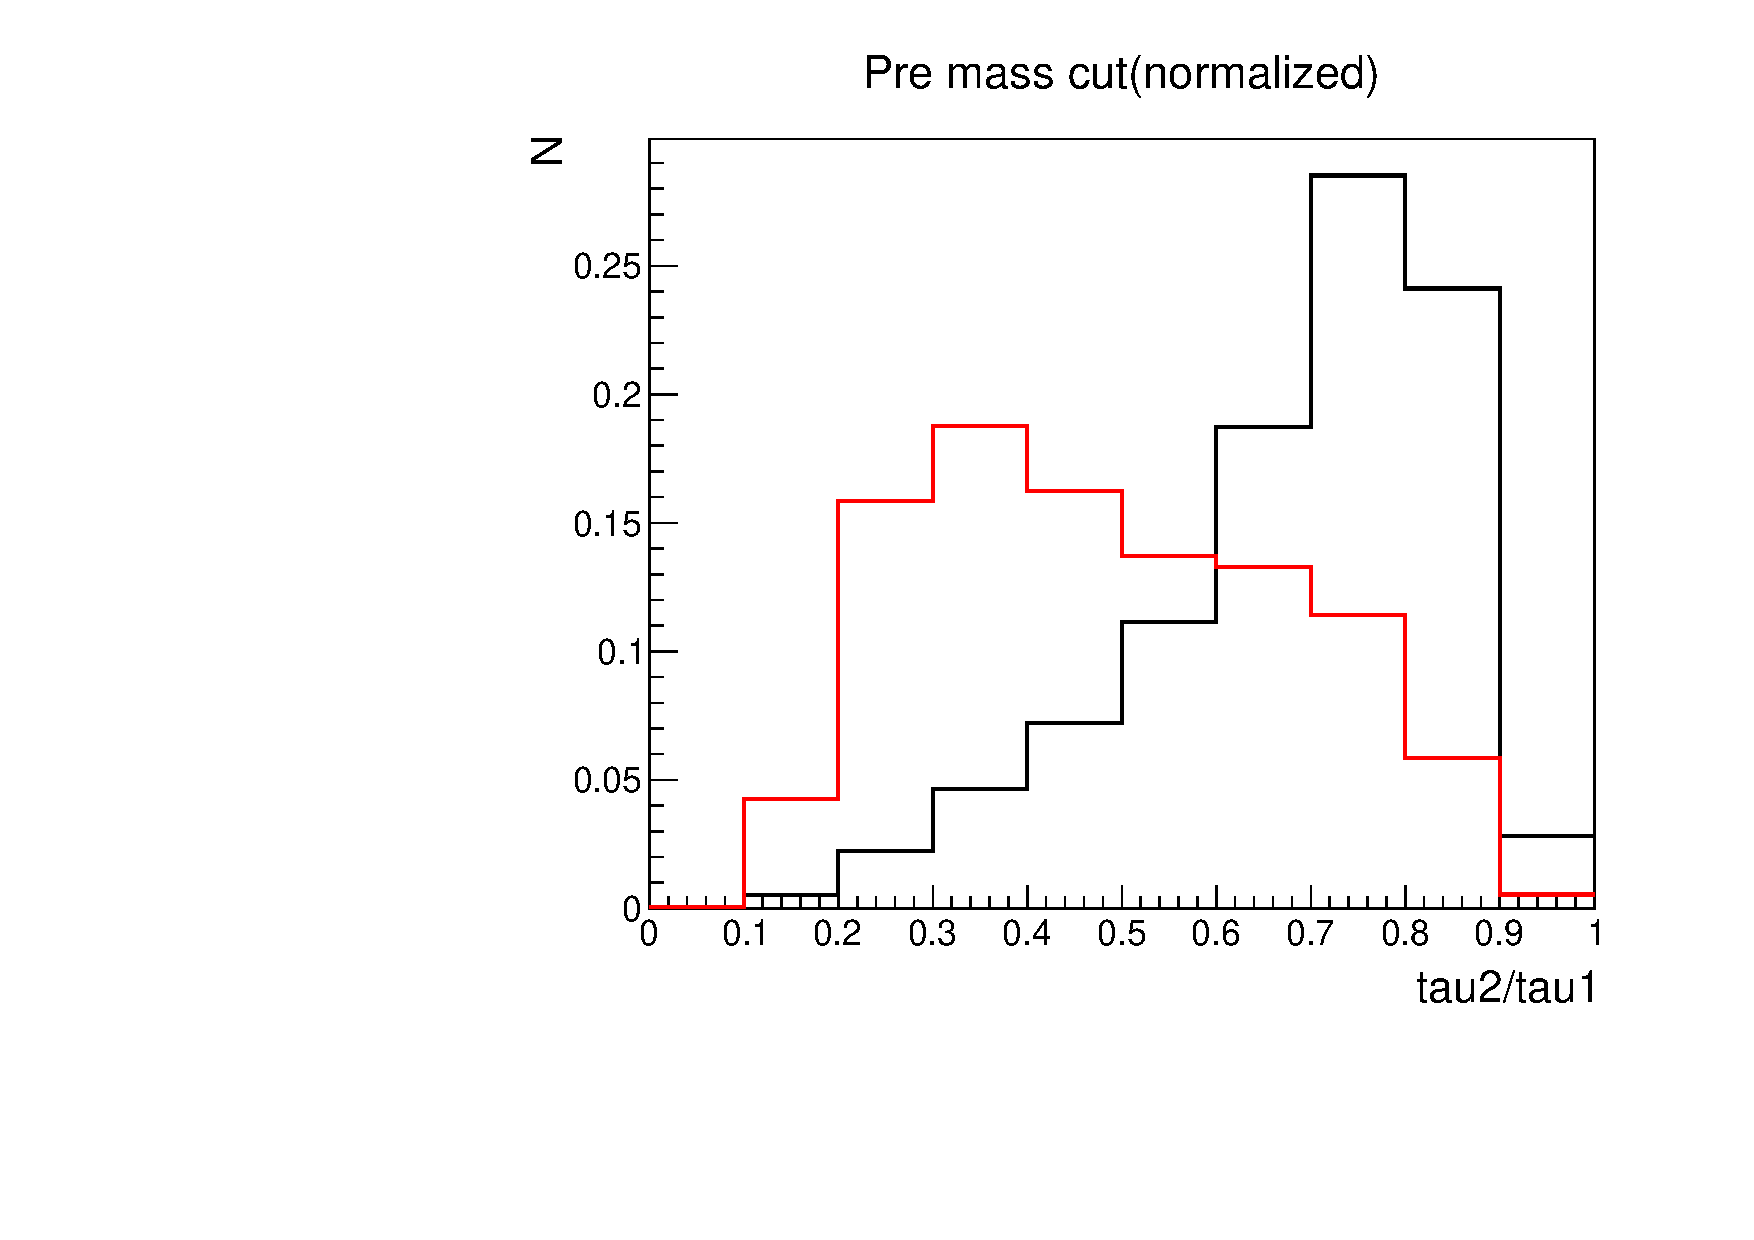
\includegraphics{EXO-12-024/figs/N-subjettiness/Signal_MC_Pre.pdf}} &
     \resizebox{0.5\linewidth}{!}{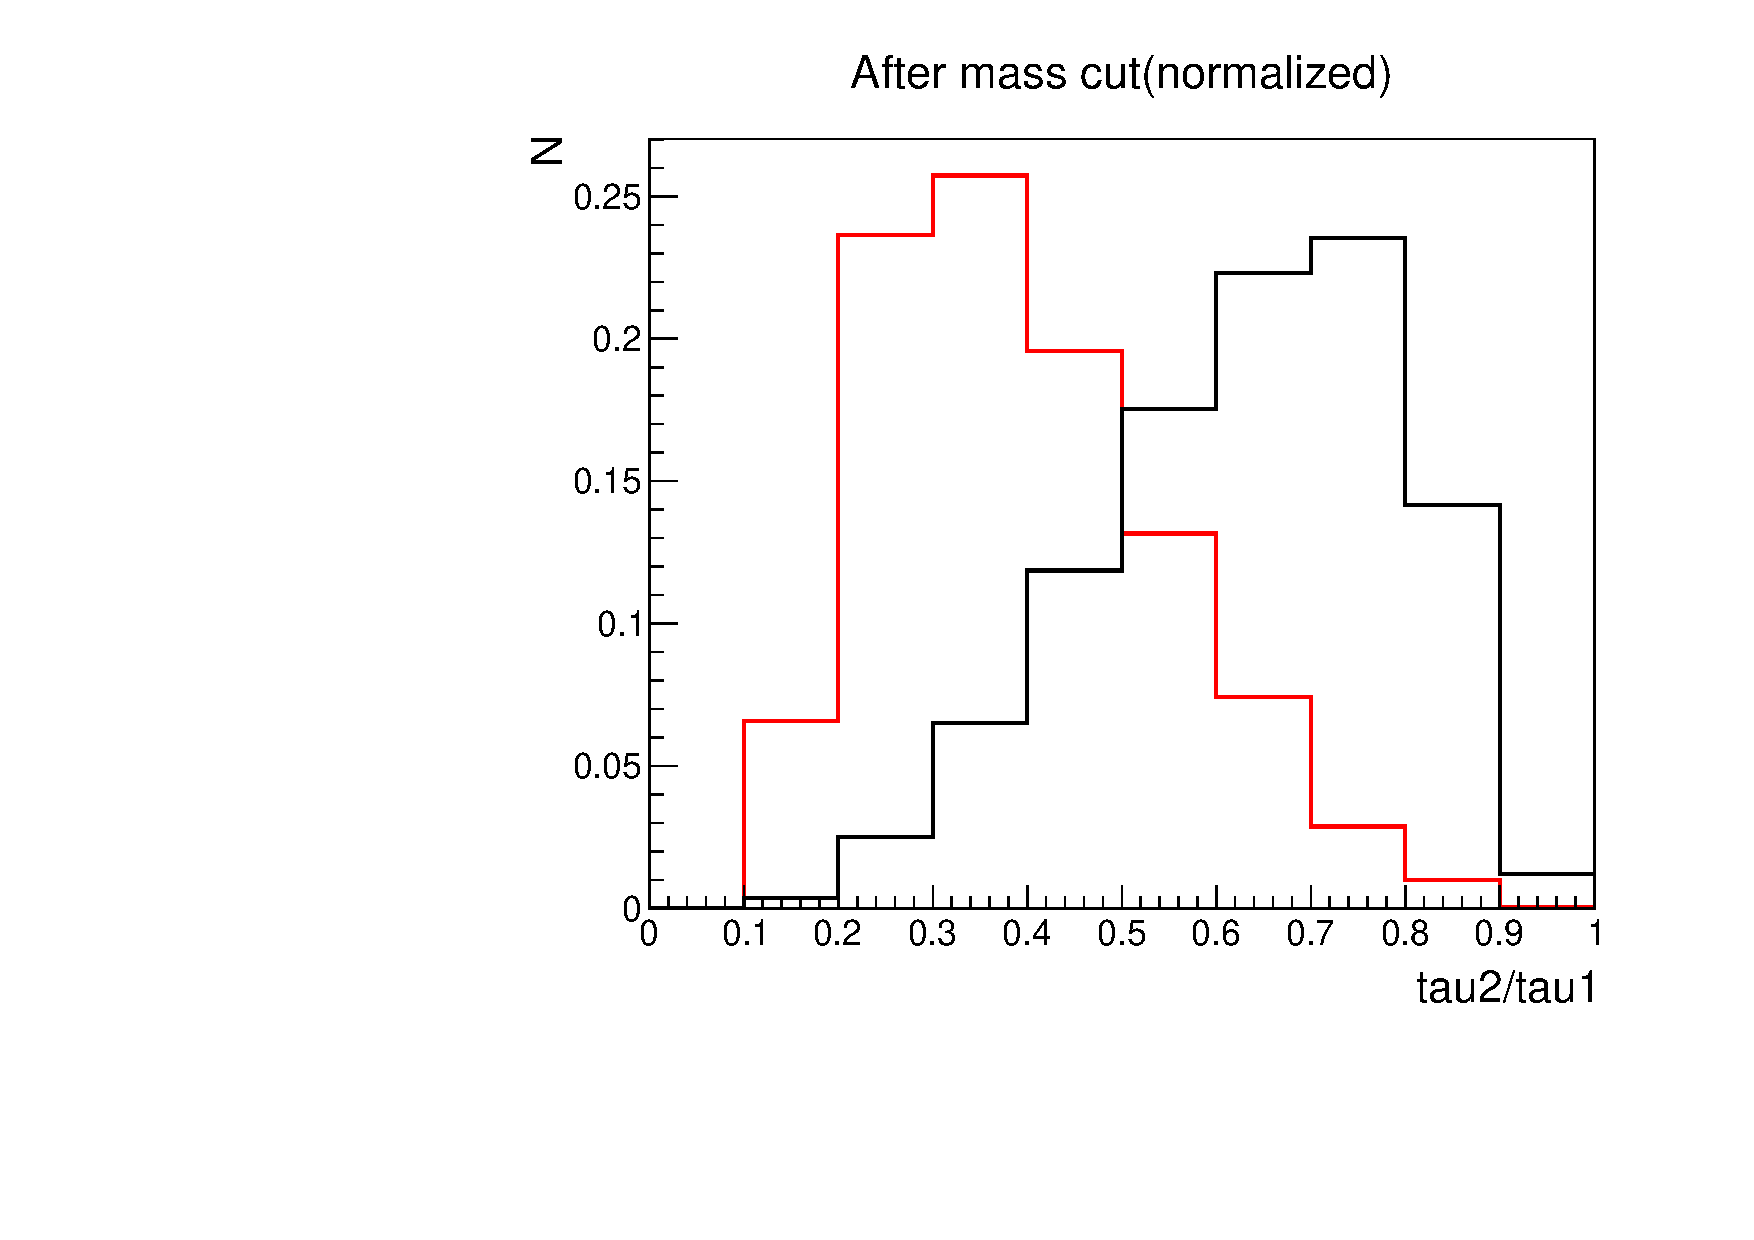
\includegraphics{EXO-12-024/figs/N-subjettiness/Signal_MC.pdf}} \\
\end{tabular}
\caption[N-subjettiness]{Comparison for $\tau_{2}/\tau_{1}$ distribution between signal (red) and background (black) before the jet mass cut (left) and after the jet mass cut applied (right). The signal MC used here is Herwig WW 1.5 TeV, and background is Herwig QCD.}
\label{fig:N-sub-mass}
\end{figure}

%\textbf{PLAN} in Fig~\ref{N-sub} and Fig~\ref{N-sub-mass}, I'm gonna add prettier plots for different signals(pythia and herwig, 1.0Tev to 3.0TeV resonance).  

%The leading two ungroomed CA8 jets to the leading two pruned CA8 jets are matched requireing $\Delta R < 0.5 $, which fails in less than 0.1\% of the events.

We select ``high purity'' $\PW/\cPZ$ jets by
requiring $\tau_{21} \leq 0.5$, while $ 0.5 <
\tau_{21} < 0.75$ defines the ``low purity'' $\PW/\cPZ$ jets.
%
The division of events with one $\PW/\cPZ$-tag follows the same delineation.
%
The events with two $\PW/\cPZ$-tagged jets are always required 
to have one high purity $\PW/\cPZ$ tag, and are similarly divided
into the ``high'' and the ``low purity'' categories depending on whether
the other $\PW/\cPZ$-tagged jet has passed the high or the low purity requirement, 
respectively.
%
The high purity category has been optimized to reach on average the
best sensitivity for all models considered in this search.  The low
purity category adds sensitivity in particular at high dijet masses
where the $\PW/\cPZ$-tagging efficiency drops along with the
background rate.

\subsection{Optimization study for the W-tagger}
\label{sec:optimal}
%\textbf{PLAN} This part we're gonna talk about what we did for the optimization search of tau2/tau1 cut. 

The cut values for the pruned jet mass and N-subjettiness were optimized based on the best expected limit.
The final cut values are a compromise between best expected limits for WW and ZZ resonances in the range between 1 and 2 TeV, because we target both of them with the same analysis.

Figure~\ref{fig:optimization0} shows the optimization of the N-subjettiness ($\tau_{21}$) or massdrop ($\mu$) cut value.
The massdrop variable was used in the 2011 version of this analysis and has been replaced by the 
N-subjettiness.
A N-subjettiness cut gives a 30\% better limit than the massdrop cut.
The $\tau_{21}<0.5$ is the best cut value for equal performance in both WW and ZZ resonances.
The expected limit changes by $<$5\% changing the $\tau_{21}$ cut value by $\pm$0.05.

\begin{figure}[htb]
\centering
\begin{tabular}{cc}
     \resizebox{0.5\linewidth}{!}{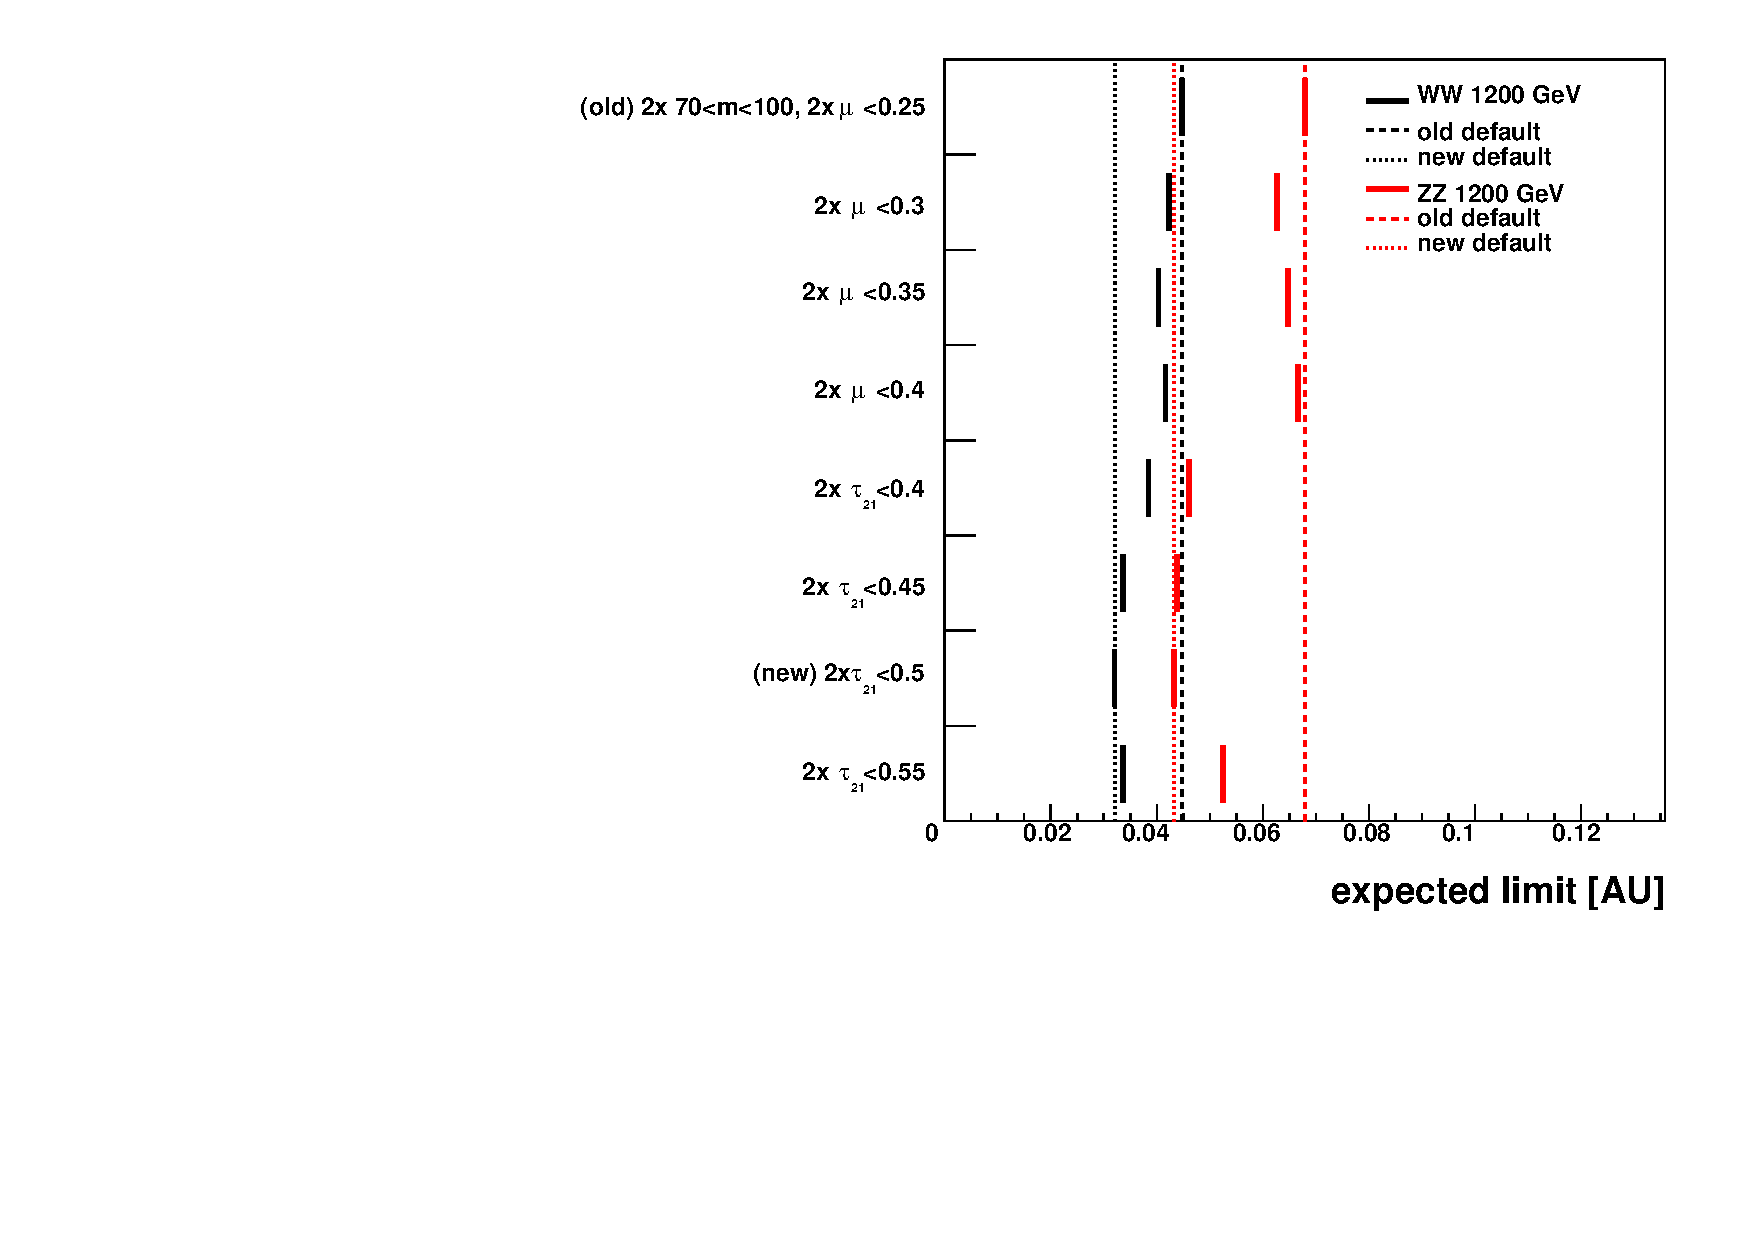
\includegraphics{EXO-12-024/figs/N-subjettiness/optimization1200_0.pdf}} &
%     \resizebox{0.5\linewidth}{!}{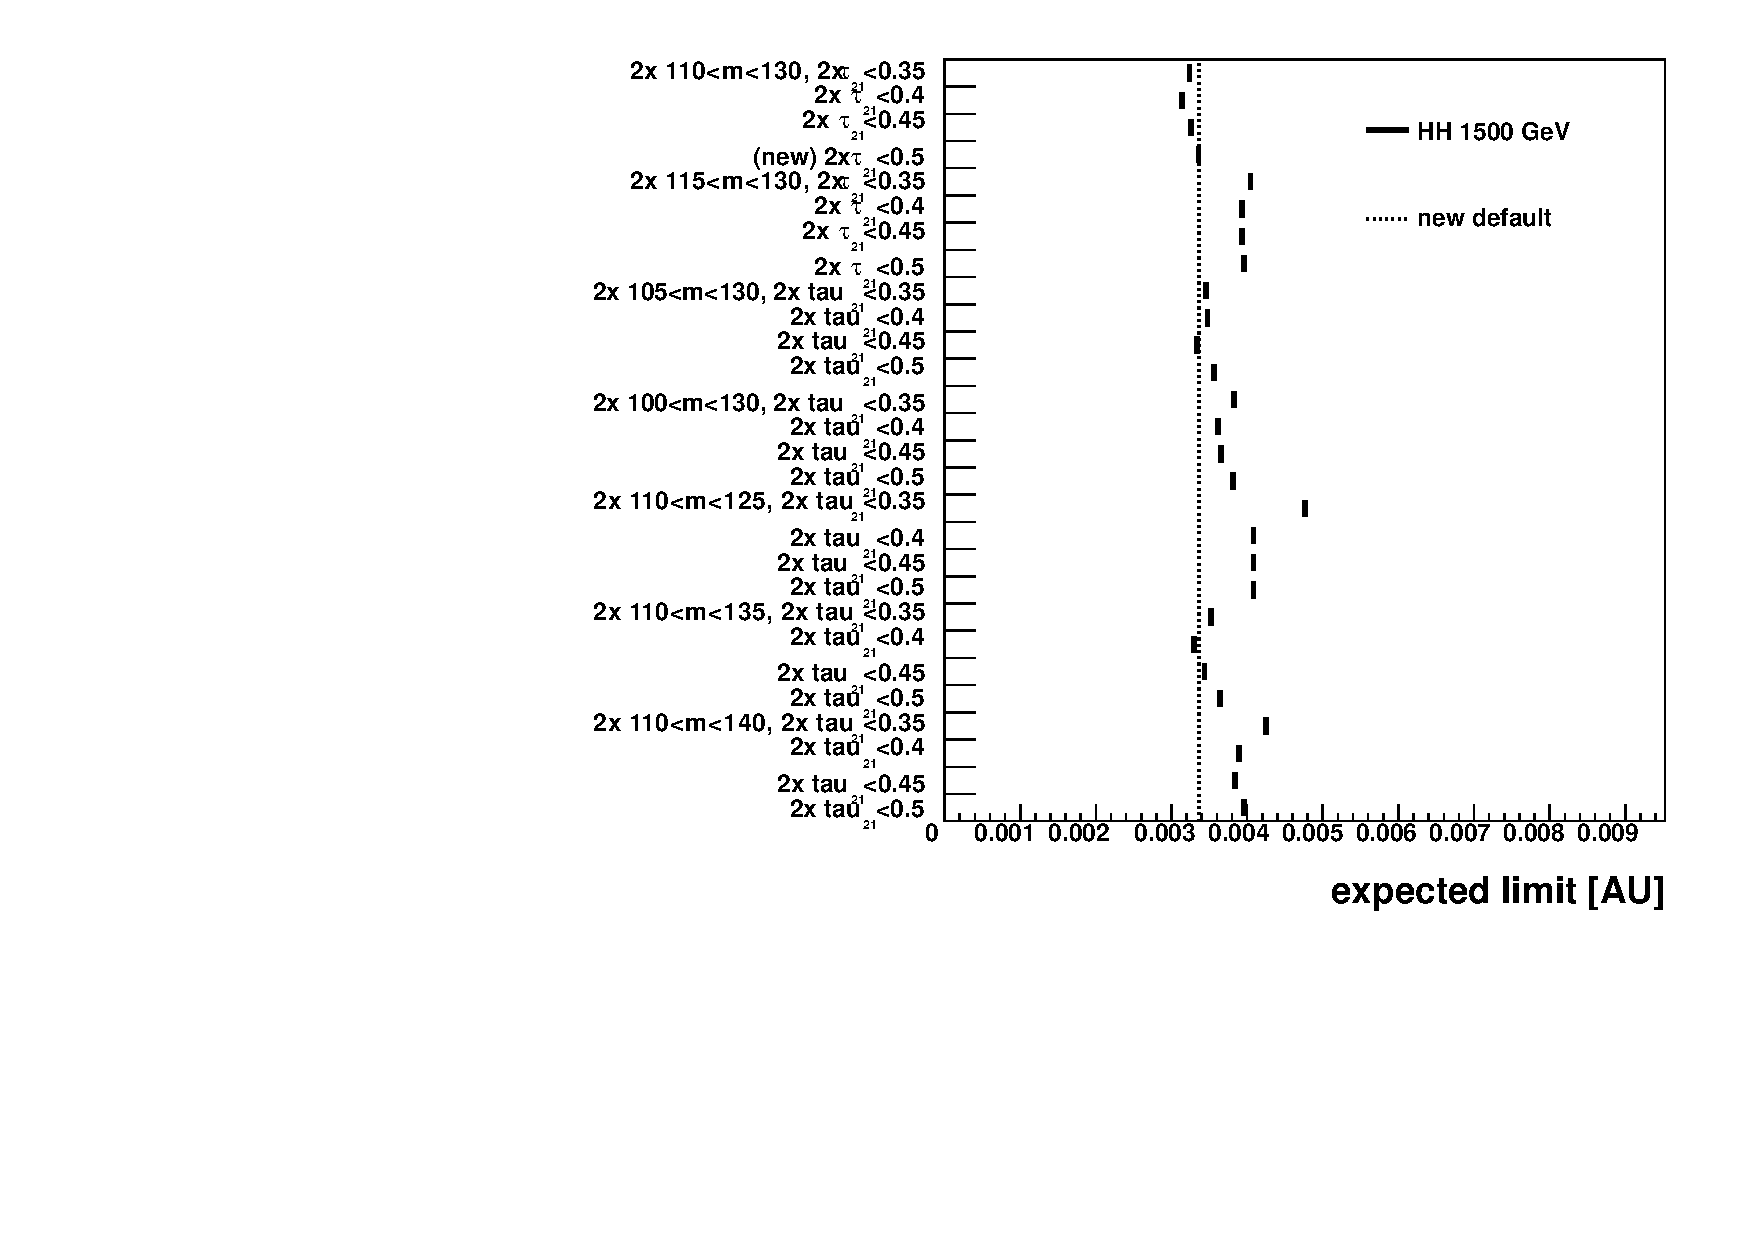
\includegraphics{figs/N-subjettiness/optimization1500_0.pdf}} &
     \resizebox{0.5\linewidth}{!}{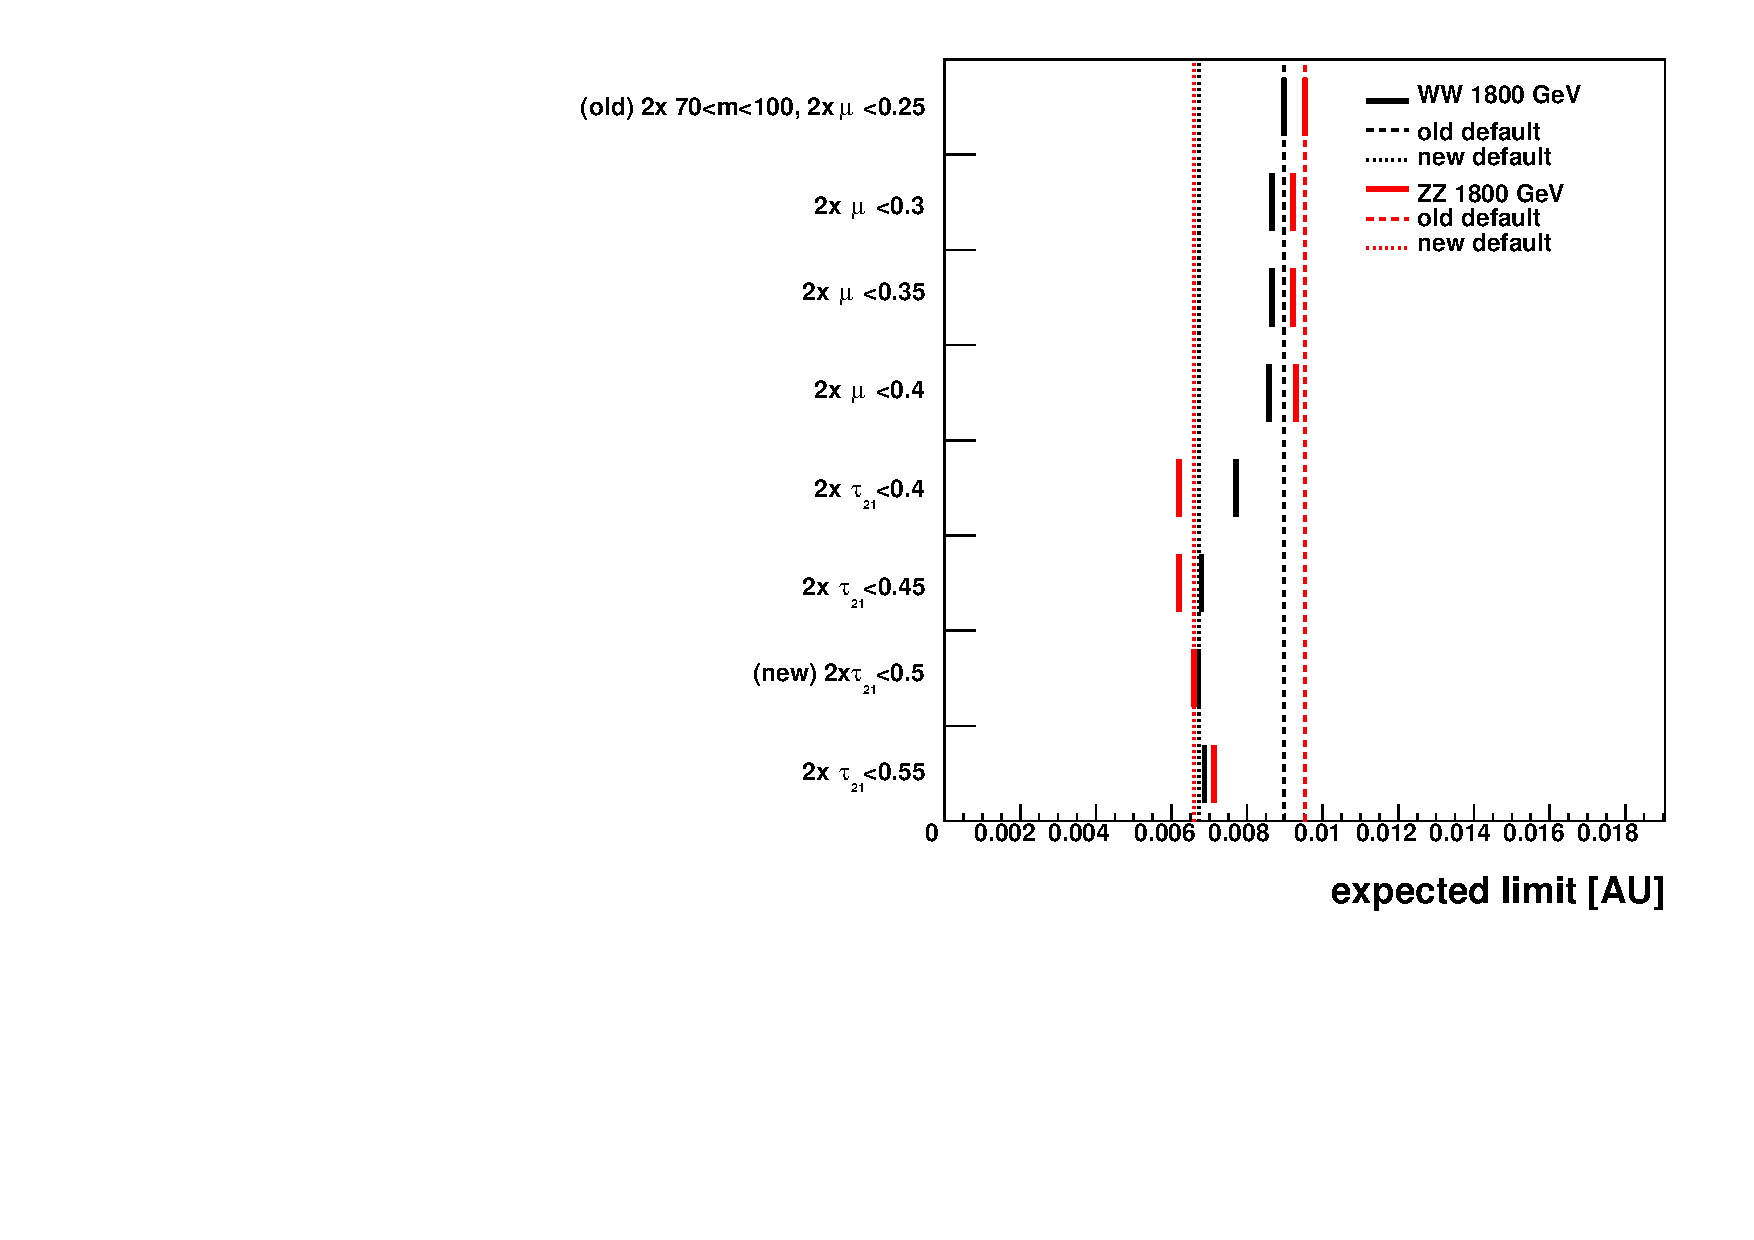
\includegraphics{EXO-12-024/figs/N-subjettiness/optimization1800_0.pdf}} \\
\end{tabular}
\caption[N-subjettiness]{Optimizataion of the N-subjettiness ($\tau_{21}$) or massdrop ($\mu$) cut value for the best expected limit.}
\label{fig:optimization0}
\end{figure}

Figure~\ref{fig:optimization1} shows the optimization of the pruned jet mass window cut.
Neither widing nor narrowing the pruned jet mass window on either side can improve the expected limit for WW and ZZ at the same time.
The jet mass window of $70 < m_\text{jet} <  100$~GeV provides best performance for WW and ZZ at the same time.

\begin{figure}[htb]
\centering
\begin{tabular}{cc}
     \resizebox{0.5\linewidth}{!}{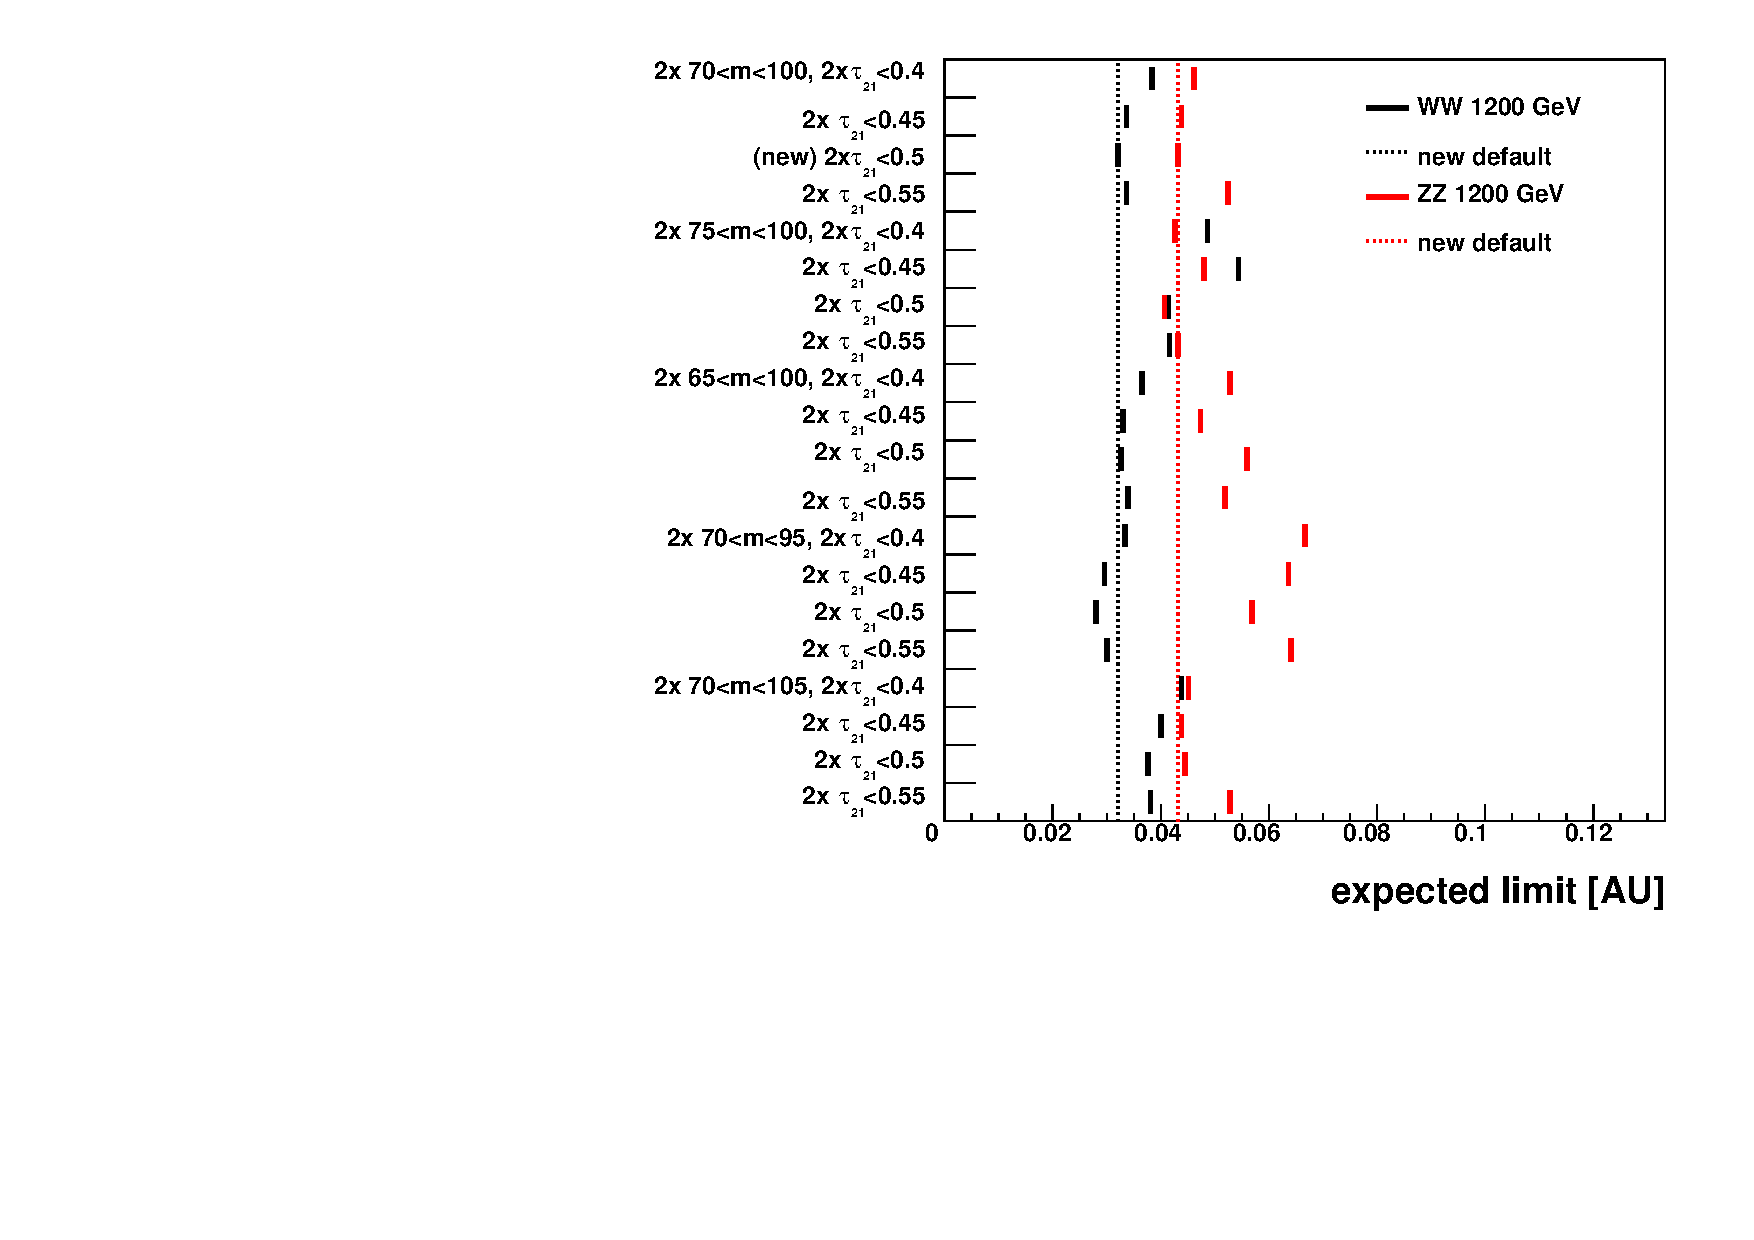
\includegraphics{EXO-12-024/figs/N-subjettiness/optimization1200_1.pdf}} &
%     \resizebox{0.5\linewidth}{!}{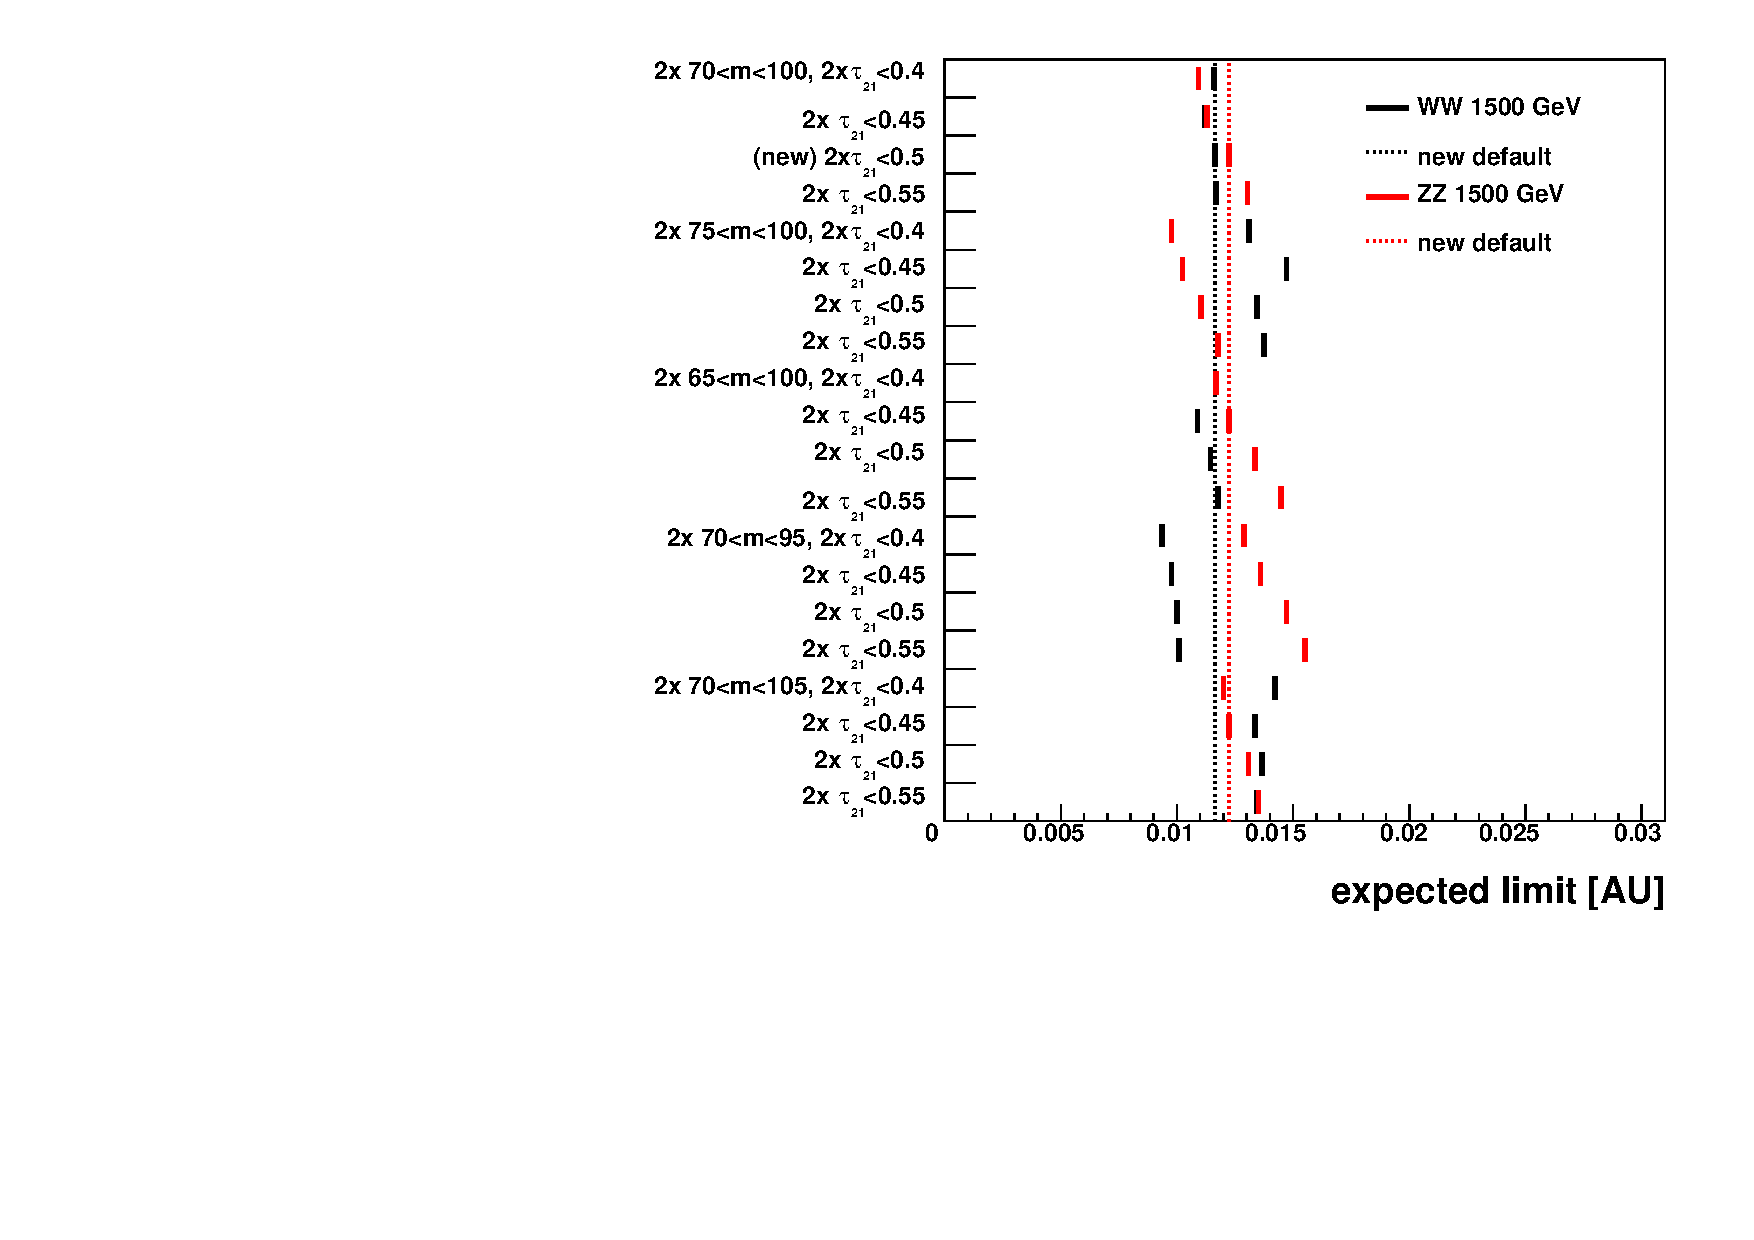
\includegraphics{figs/N-subjettiness/optimization1500_1.pdf}} &
     \resizebox{0.5\linewidth}{!}{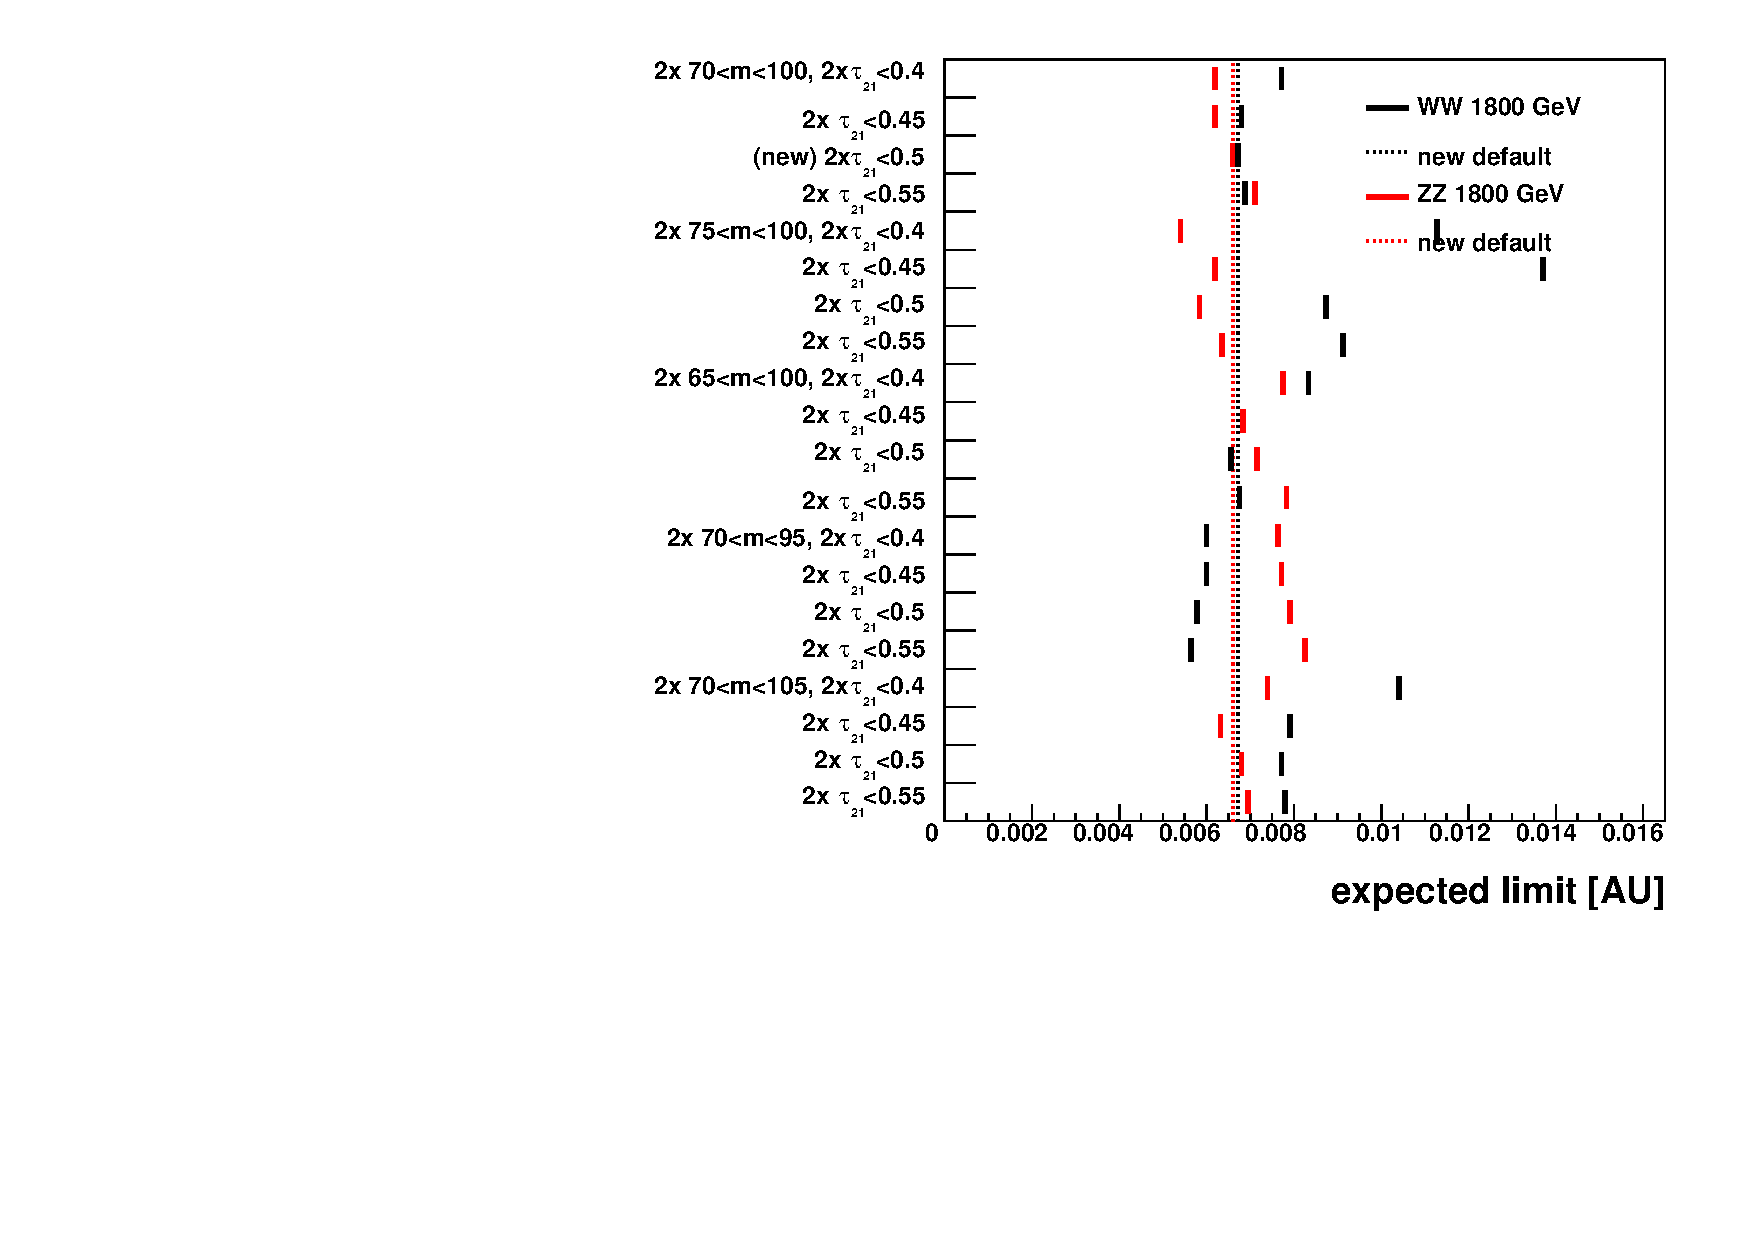
\includegraphics{EXO-12-024/figs/N-subjettiness/optimization1800_1.pdf}} \\
\end{tabular}
\caption[N-subjettiness]{Optimizataion of the pruned jet mass window cut for the best expected limit.}
\label{fig:optimization1}
\end{figure}

Figure~\ref{fig:optimization2} shows the dependency of the expected limit on the jet algorithm used for the resonance mass reconstruction.
It is found that AK5, AK7 and CA8 show almost the same performance.
This analysis switched since 2011 from AK5 to CA8 for consistency with other similar analyses. 
%EXO-12-021 and EXO-12-022.

\begin{figure}[htb]
\centering
\begin{tabular}{cc}
%     \resizebox{0.5\linewidth}{!}{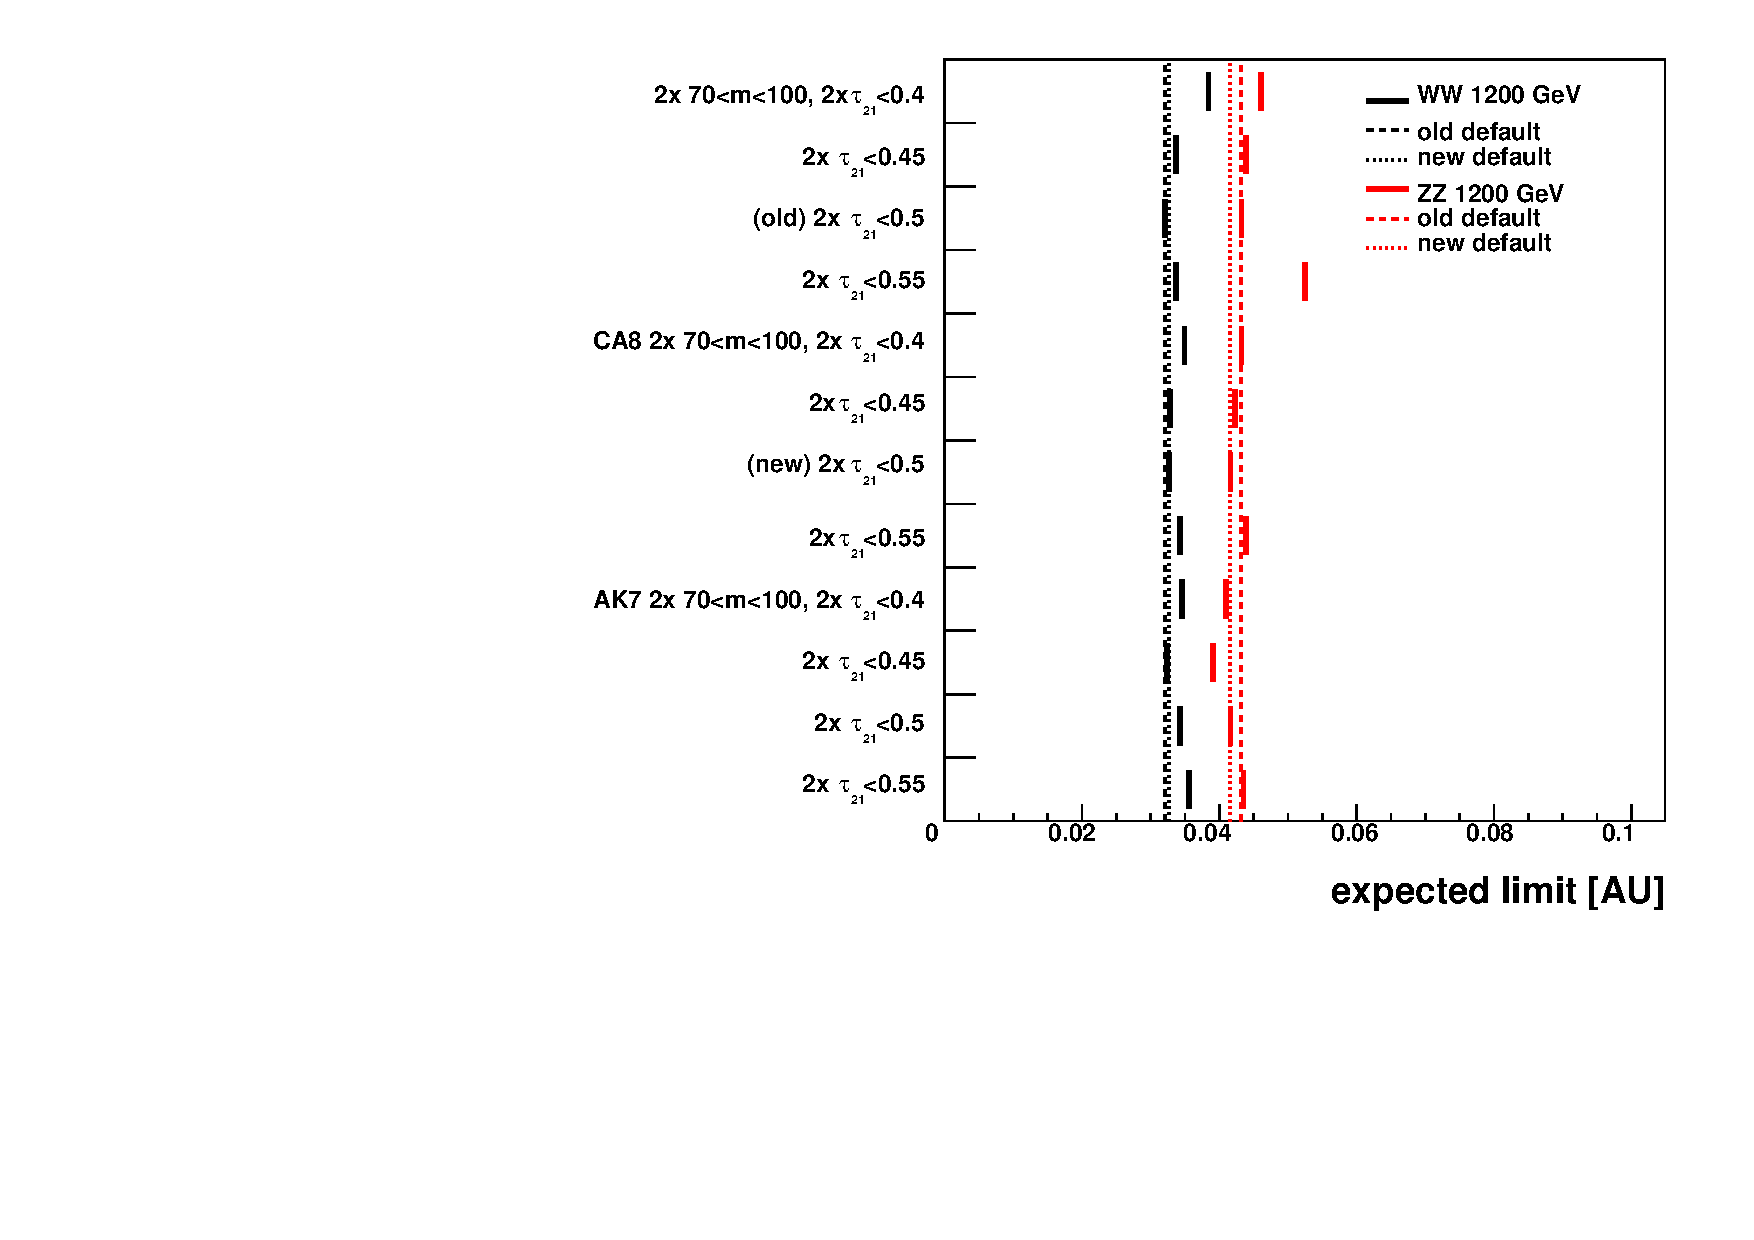
\includegraphics{figs/N-subjettiness/optimization1200_2.pdf}} &
%     \resizebox{0.5\linewidth}{!}{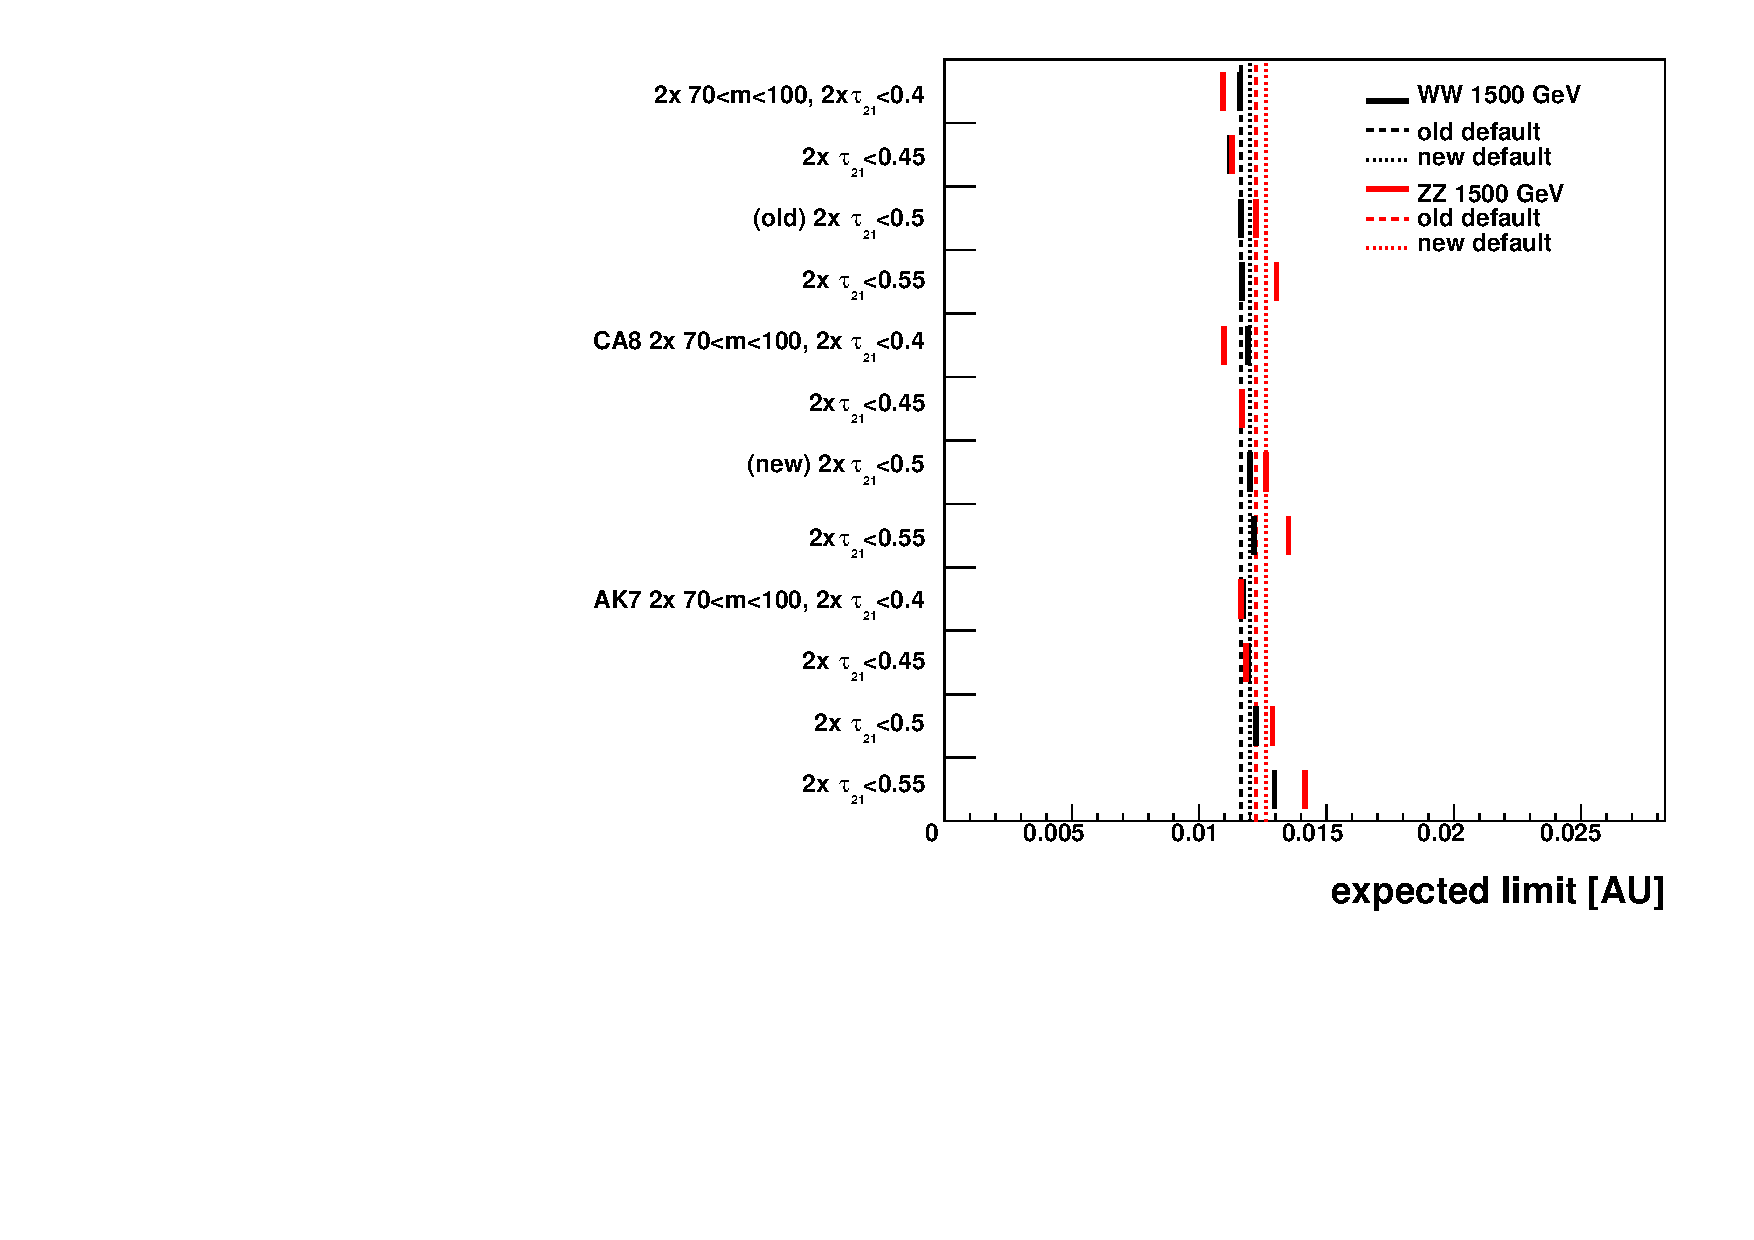
\includegraphics{figs/N-subjettiness/optimization1500_2.pdf}} &
     \resizebox{0.5\linewidth}{!}{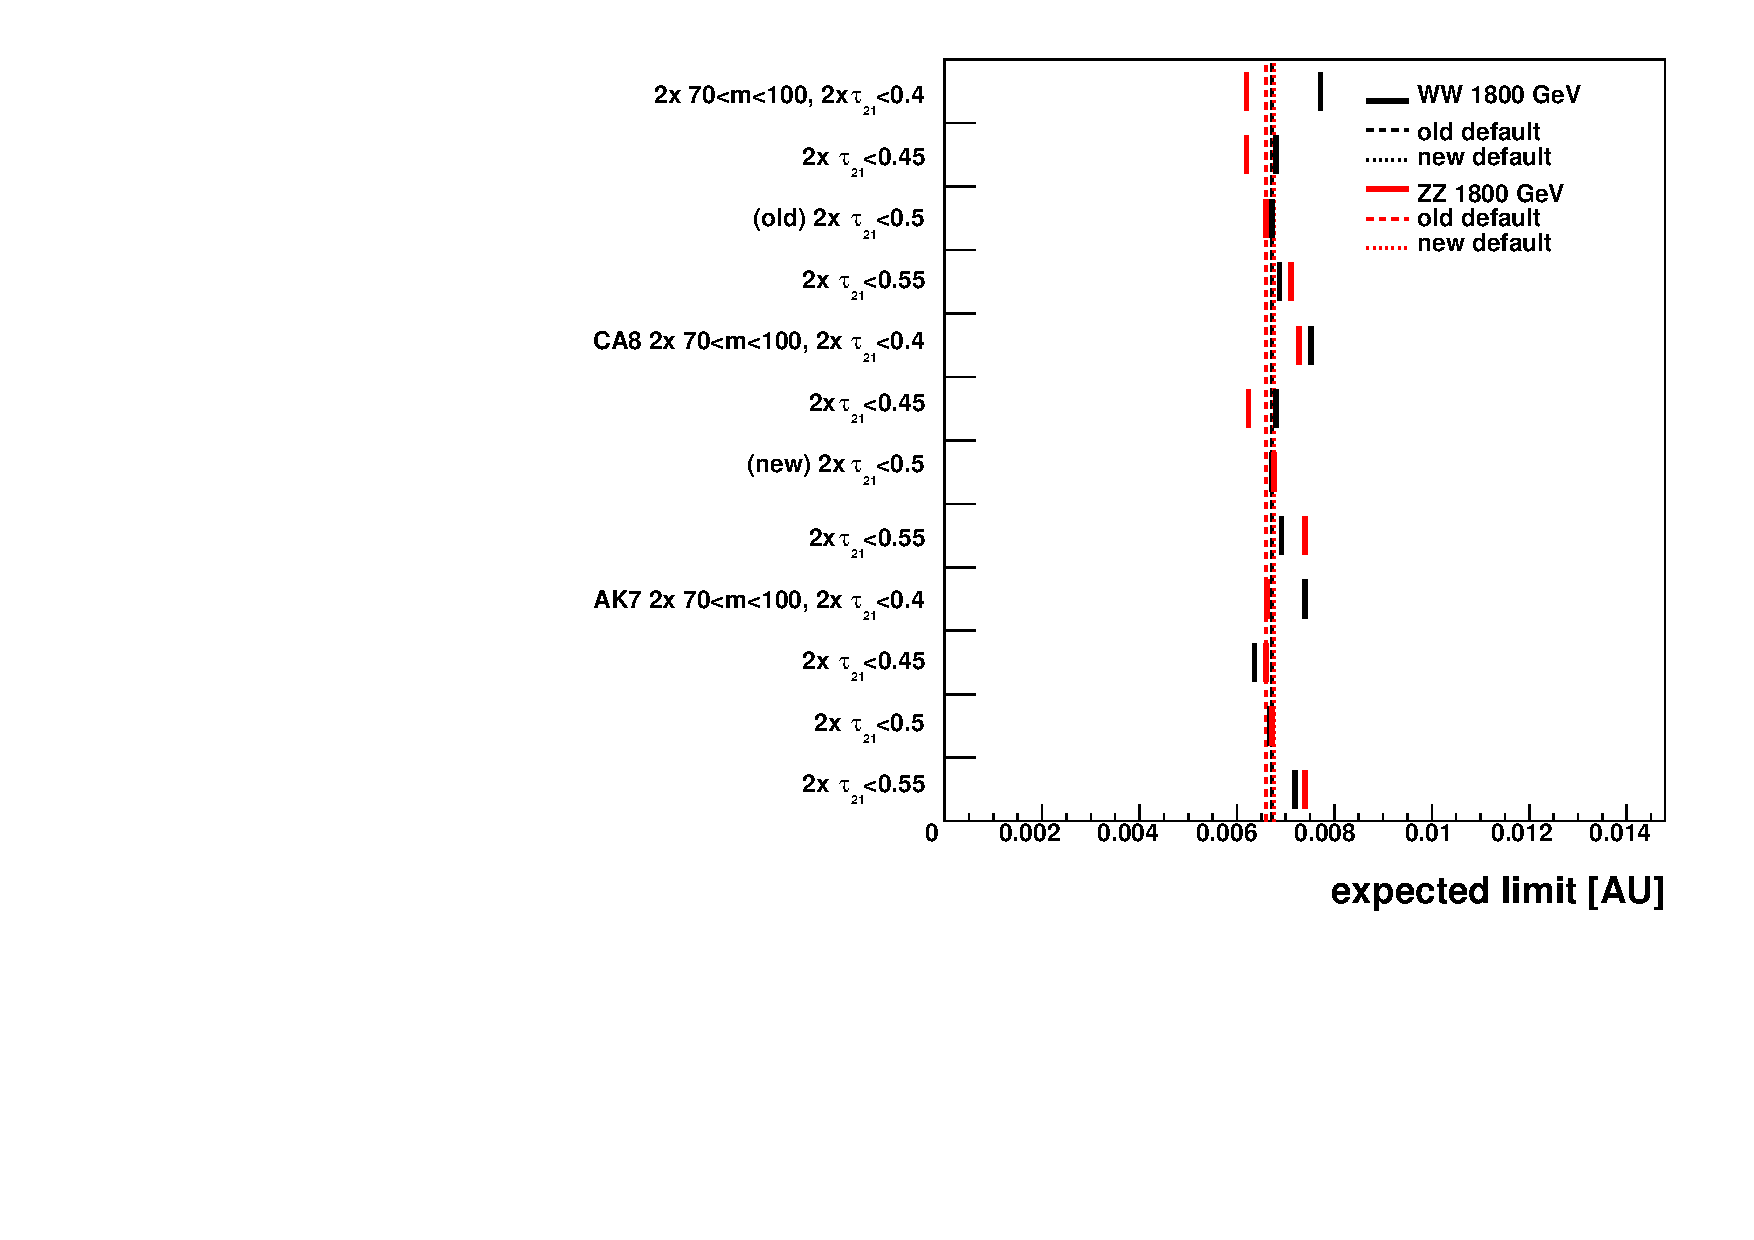
\includegraphics{EXO-12-024/figs/N-subjettiness/optimization1800_2.pdf}} \\
\end{tabular}
\caption[N-subjettiness]{Comparison of expected limit for different jet algorithms.}
\label{fig:optimization2}
\end{figure}

%\newpage
%\section{Benchmark model for a vector triplet}
%
%Information about the signal models used  is in Table~\ref{table:signalModels}

%\begin{table}[htbp]
%\resizebox{\textwidth}{!}{
%\begin{tabular}{|r|r|r|r|r|r|r|}
%\hline
%\multicolumn{1}{|l|}{M(GeV)} & \multicolumn{1}{l|}{width(GeV)} & \multicolumn{1}{l|}{BR(Z'$\to$WW)} & \multicolumn{1}{l|}{BR(Z'$\to$HZ ) } & \multicolumn{1}{l|}{BR(W'$\to$ZW)} & \multicolumn{1}{l|}{BR(W'$\to$HW )} & \multicolumn{1}{l|}{X-section(pb)} \\ \hline
%800 & 32.03 & 0.4139 & 0.5672 & 0.4287 & 0.5528 & 3.17E-01 \\ 
%900 & 32.97 & 0.4393 & 0.534 & 0.4513 & 0.5223 & 2.39E-01 \\ 
%1000 & 34.95 & 0.4506 & 0.5176 & 0.4603 & 0.5079 & 1.65E-01 \\ 
%1500 & 47.94 & 0.4665 & 0.4893 & 0.4709 & 0.4849 & 2.44E-02 \\ 
%2000 & 62.2 & 0.4698 & 0.4815 & 0.4723 & 0.4791 & 4.01E-03 \\ 
%2500 & 76.81 & 0.471 & 0.4783 & 0.4726 & 0.4767 & 7.08E-04 \\ 
%3000 & 91.57 & 0.4716 & 0.4765 & 0.4727 & 0.4754 & 1.26E-04 \\ 
%\hline
%\end{tabular}
%}
%\caption{Summary of signal models.}
%\label{table:signalModels}
%\end{table}


\section{Data and Monte Carlo samples}
\label{sec:data_and_mc_samples}


The data sample of proton-proton collisions at $\sqrt{s}=8$~\TeVcc was collected in 2012 and corresponds to
an integrated luminosity of \intlumi.
The datasets and also the certifications
used are summarized in Table~\ref{table:dataset}. 
The dijet sample is dominated by light flavored and gluon jets, which we denote as 
the "QCD background".  
%The QCD background is obtained from data by fitting an
%analytic parameterization of the dijet invariant mass distribution.

We list part of our monte carlo simulated signal(from 1 \TeVcc to 2.6 \TeVcc) 
in 
Table~\ref{table:Hww}. 
Signal samples are generated exclusively of the specific 
Higgs decay mode and W/Z decay mode. 
Model parameters and detailed cross sections are summarized in 
Appendix~\ref{appendix:modelParam}.
The matrix element is calculated with Madgraph~5.1.5.11~\cite{madgraph}. 
% in Table~\ref{table:Hbb} and 
%Table~\ref{table:Hww}, 
The signals of interest,
are showered and hadronized with 
\PYTHIA~6.426~\cite{pythia}, and \HERWIG{++} 2.5.0~\cite{herwig}, 
using simulation of the
CMS detector, based on \GEANTfour~\cite{refGEANT}. Tune
Z2*~\cite{bib_tunez1}
is used in \PYTHIA, while the version 23 tune~\cite{herwig} is used in
\HERWIG{++}. The CTEQ61L~\cite{cteq} parton distribution functions
(PDF) are used for \PYTHIA and the MRST2001~\cite{mrst} leading-order
(LO) PDF for \HERWIG{++}
%All Monte Carlo events are fully simulated and reconstructed via the Geant4-based CMS simulation
% and reconstruction software. 
%Information about the signal models used 
%is in Table~\ref{table:signalModels}
W' and Z' are generated with resonance widths
at $\approx$4\% of the resonance mass, slightly smaller than
the experimental resolution in $m_\mathrm{jj}$ for resonance masses
considered in the analysis. Samples showered from
 \PYTHIA are used in the analysis. %On the other hand, to compare
%the effect of hadronization,  \HERWIG{++} is therefore used
%to retrieve the difference.
While, samples from \HERWIG{++} are used to evaluate the systematic 
uncertainty by comparing the difference of hadronization from \PYTHIA.

%All simulated samples are passed through the standard CMS event
%reconstruction software.



%\begin{table}[htbp]
%\begin{tabular}{|r|r|r|r|r|r|r|}
%\hline
%\multicolumn{1}{|l|}{M(GeV)} & \multicolumn{1}{l|}{width(GeV)} & \multicolumn{1}{l|}{BR(Z'$\to$WW)} & \multicolumn{1}{l|}{BR(Z'$\to$HZ ) } & \multicolumn{1}{l|}{BR(W'$\to$ZW)} & \multicolumn{1}{l|}{BR(W'$\to$HW )} & \multicolumn{1}{l|}{X-section(pb)} \\ \hline
%800 & 32.03 & 0.4139 & 0.5672 & 0.4287 & 0.5528 & 3.17E-01 \\ 
%900 & 32.97 & 0.4393 & 0.534 & 0.4513 & 0.5223 & 2.39E-01 \\ 
%1000 & 34.95 & 0.4506 & 0.5176 & 0.4603 & 0.5079 & 1.65E-01 \\ 
%1500 & 47.94 & 0.4665 & 0.4893 & 0.4709 & 0.4849 & 2.44E-02 \\ 
%2000 & 62.2 & 0.4698 & 0.4815 & 0.4723 & 0.4791 & 4.01E-03 \\ 
%2500 & 76.81 & 0.471 & 0.4783 & 0.4726 & 0.4767 & 7.08E-04 \\ 
%3000 & 91.57 & 0.4716 & 0.4765 & 0.4727 & 0.4754 & 1.26E-04 \\ 
%\hline
%\end{tabular}
%\caption{Summary of signal models.}
%\label{table:signalModels}
%\end{table}



\begin{table}[htb]
\begin{center}
\begin{tabular}{ |l| }
\hline
Dataset                                 \\
\hline
/Jet/Run2012A-22Jan2013-v1/AOD  \\
/JetHT/Run2012B-22Jan2013-v1/AOD  \\
/JetHT/Run2012C-22Jan2013-v1/AOD  \\
/JetHT/Run2012D-22Jan2013-v1/AOD  \\
\hline
\end{tabular} 
\end{center}
\caption{Summary of 8~\TeVcc collision data used in this analysis. 
The certification file used for these data is 
{\tt Cert\_190456-208686\_8TeV\_22Jan2013ReReco\_Collisions12\_JSON.txt
}.
}
\label{table:dataset}
\end{table}

\begin{table}[htb]
\begin{center}
\begin{tabular}{ |l|c|r|r| }
\hline
Process     & mass ($\GeVcc$) & Events & X-sec[pb] \\
\hline
Z' $\to$ HZ & 1000   &20000   & 8.56E-02 \\
 & 1500   &20000              & 1.19E-02 \\
 & 2000   &20000              & 1.93E-03 \\
 & 2500  &20000               & 3.39E-04  \\\hline
%W' $\to$ H(ww $\to$ qqqq)W(qq)(m=750$\GeVcc$) &Madgraph   &20000   &4.071E+01  \\
W' $\to$ HW& 1000   &20000   &  1.71E-01  \\
 & 1500 &20000               &  2.55E-02  \\
 & 2000 &20000               &  4.25E-03  \\
 & 2500  &20000              &  7.31E-04  \\
\hline
\end{tabular}
\end{center}
\caption{Examples of the simulated Monte Carlo samples used in this analysis for process
 V' $\to$ VH. Cross sections are calculated from 
production cross sections of V' times its BR(W' $\to$HW or Z' $\to$ HZ). 
 These samples are generated using Madgrap5 and hadronized with Pythia6. }
\label{table:Hww}
\end{table}


\iffalse

\begin{table}[htb]
\begin{center}
\begin{tabular}{ |l|c|r|r| }
\hline
Process           & mass ($\GeVcc$) & Events & X-sec[pb] \\
\hline
Z' $\to$ H(bb)Z(qq) & 1000  &20000   & 3.45E-02 \\
 & 1500     &20000   & 4.81E-03 \\
 & 2000    &20000   & 7.79E-04  \\
 & 2500    &20000   & 1.37E-04 \\\hline
%W' $\to$ H(bb)W(qq)(m=750$\GeVcc$) &Madgraph   &20000   &4.071E+01  \\
W' $\to$ H(bb)W(qq)& 1000  &20000   & 3.28E-02 \\
 & 1500    &20000   & 4.61E-03 \\
 & 2000    &20000   & 7.50E-04 \\
 & 2500     &20000   & 1.32E-04 \\
\hline
\end{tabular}
\end{center}
\caption{Examples of the simulated Monte Carlo samples used in this analysis for process
 Z'/W'$\to$Z/W(qq) + H(bb). Those samples was generated using Madgrap5 and hadronized with Pythia6.}
\label{table:Hbb}
\end{table}

\begin{table}[htb]
\begin{center}
\begin{tabular}{ |l|c|r|r| }
\hline
Process     & mass ($\GeVcc$) & Events & X-sec[pb] \\
\hline
Z' $\to$ H(ww $\to$ qqqq)Z(qq) & 1000   &20000   & 5.88E-03 \\
 & 1500   &20000   & 8.19E-04 \\
 & 2000   &20000   & 1.33E-04 \\
 & 2500  &20000   & 2.33E-05 \\\hline
%W' $\to$ H(ww $\to$ qqqq)W(qq)(m=750$\GeVcc$) &Madgraph   &20000   &4.071E+01  \\
W' $\to$ H(ww $\to$ qqqq)W(qq)& 1000   &20000   & 5.58E-03 \\
 & 1500 &20000   & 7.85E-04  \\
 & 2000 &20000   & 1.28E-04 \\
 & 2500  &20000   & 2.24E-05 \\
\hline
\end{tabular}
\end{center}
\caption{Examples of the simulated Monte Carlo samples used in this analysis for process
 Z'/W'$\to$Z/W(qq) + H(ww $\to$ qqqq). Those samples was generated using Madgrap5 and hadronized with Pythia6.}
\label{table:Hww}
\end{table}

\fi



%\newpage

\section{Trigger}
\label{sec:trigger}


Events are selected if one of the following triggers has fired: HLT\_HT750, HLT\_PFHT650, HLT\_PFNoPUHT650,
HLT\_FatDiPFJetMass750\_DR1p1\_Deta1p5.  All versions of each of these triggers are used. None of these triggers are prescaled druing the 2012 data taking period. HLT\_PFNoPUHT650 trigger is used for the data set after the RunC(including RunC), while HLT\_PFHT650
trigger is only used for RunA and RunB data sets. 


Figure~\ref{fig:trigger efficiencies part1}, Figure~\ref{fig:trigger efficiencies part2}, and Figure~\ref{fig:trigger efficiencies part3} show the trigger efficiencies of the OR of the highest threshold HLT\_PFHT650 trigger and the HLT\_FatJetMass trigger w.r.t. an OR of the lower threshold HLT\_HT550 trigger. From the plot, the trigger is $99\%$ effiecient above 890\GeVcc for the untagged, single tagged and double tagged data. 


\begin{figure}[htb]
\centering
     \resizebox{0.75\linewidth}{!}{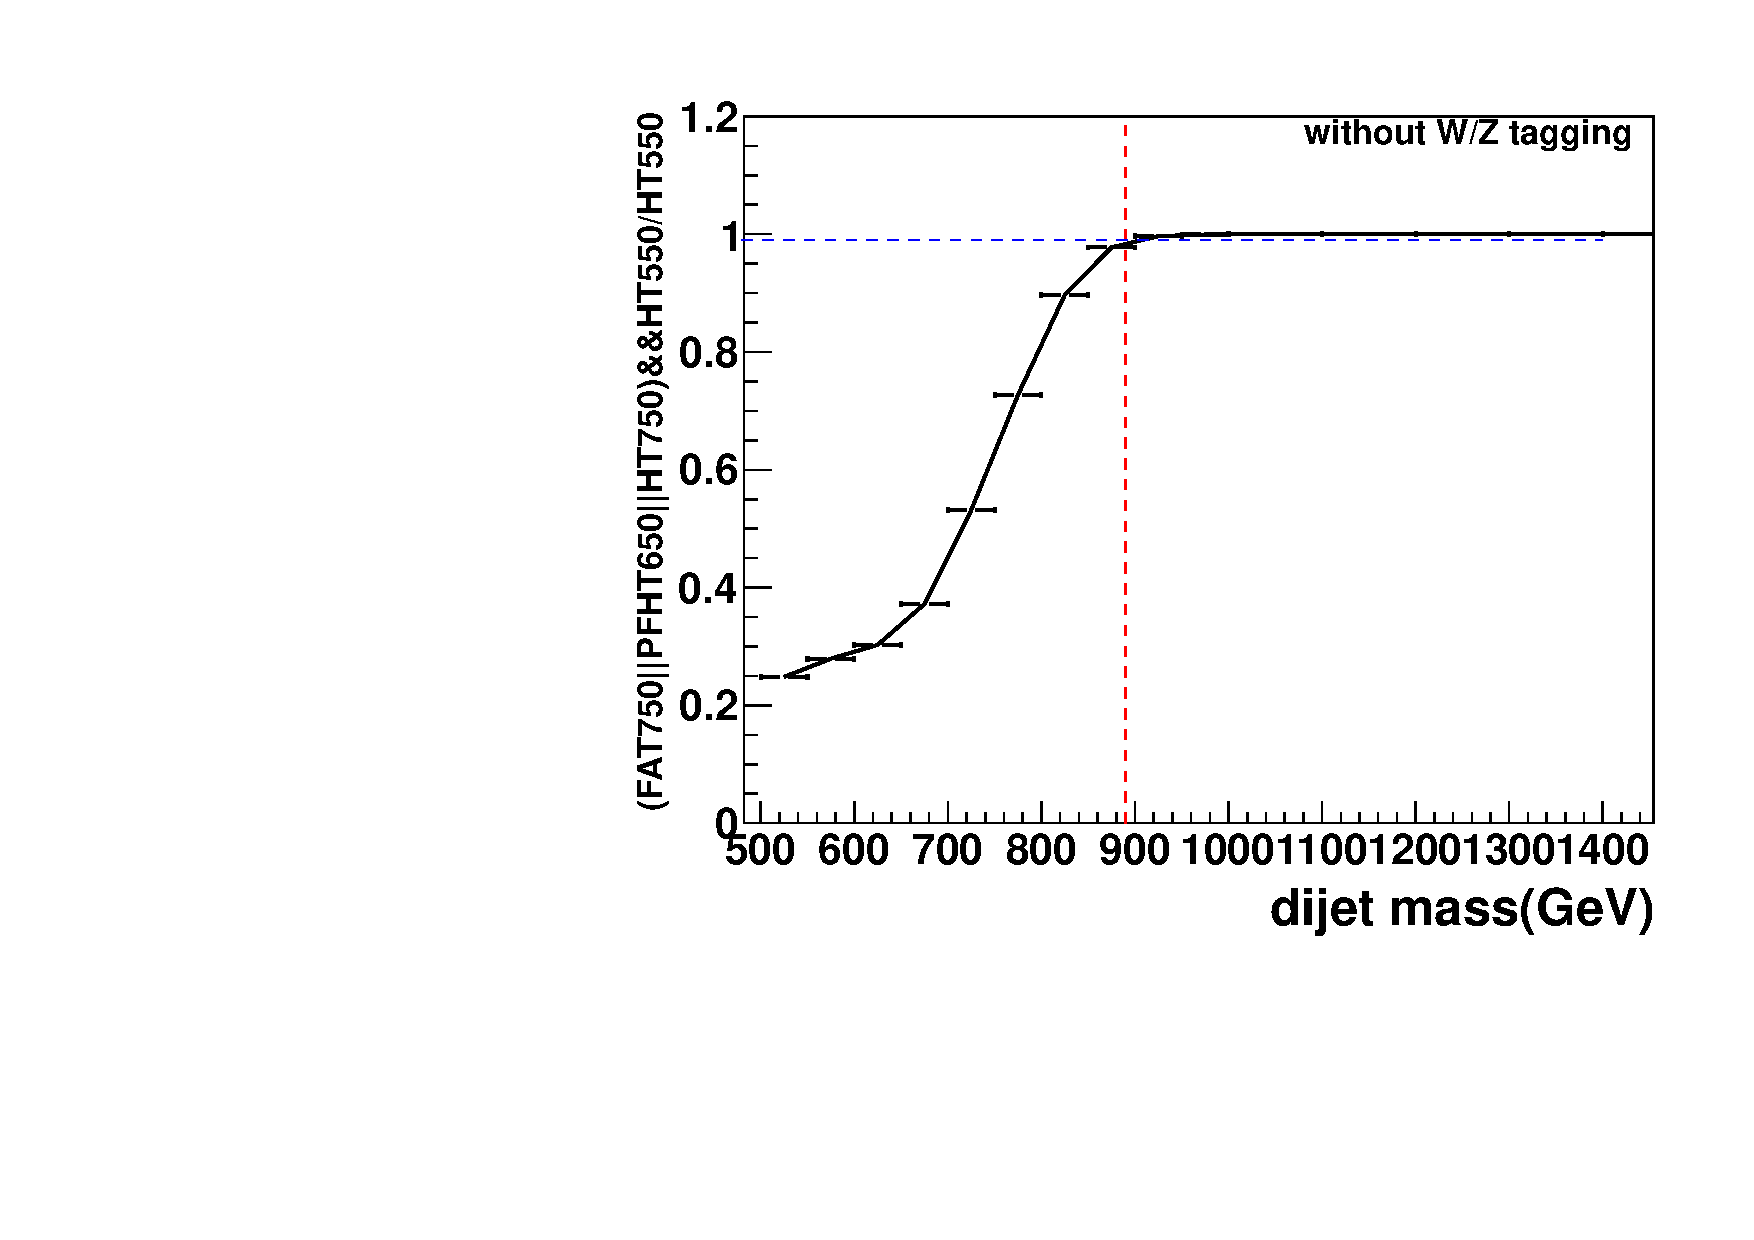
\includegraphics{EXO-12-024/figs/trigger-eff/Dataeff_withouttagging.pdf}} \\   
\caption[Trigger efficiencies]{Trigger efficiency for untagged data of FAT\_750$\parallel$HLT\_PF(NoPU)HT650$\parallel$HLT\_HT750 measured using data collected by lower threshold $H_T550$ trigger. The dash red line is positioned at $m_{jj}$ equal $890 GeV$, the blue line is at efficiency at 99$\%$. }
  \label{fig:trigger efficiencies part1}
\end{figure}

\begin{figure}[htb]
\centering
     \resizebox{0.75\linewidth}{!}{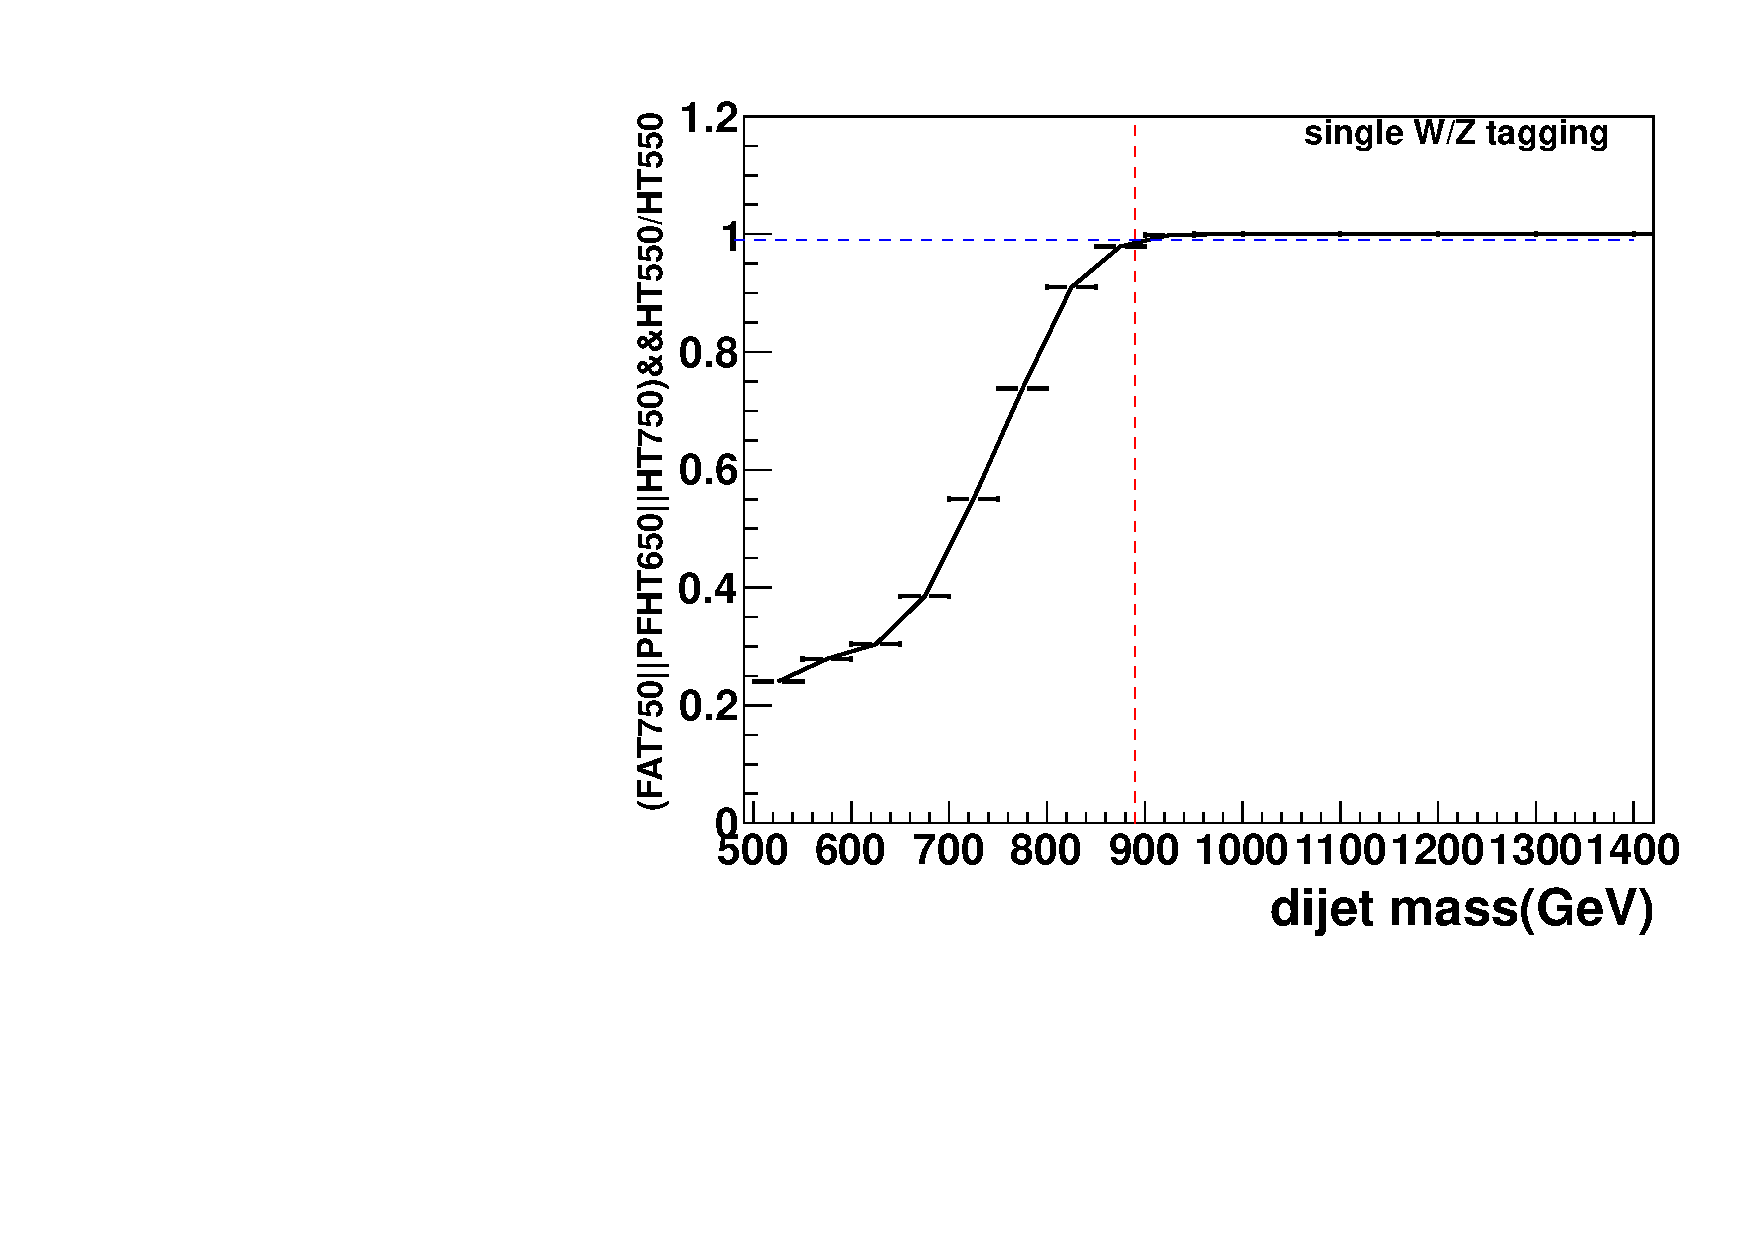
\includegraphics{EXO-12-024/figs/trigger-eff/Dataeff_singletagging.pdf}}  \\
\caption[Trigger efficiencies]{Trigger efficiency for single tagged data of FAT\_750$\parallel$HLT\_PF(NoPU)HT650$\parallel$HLT\_HT750 measured using data collected by lower threshold $H_T550$ trigger. The dash red line is positioned at $m_{jj}$ equal $890 GeV$, the blue line is at efficiency at 99$\%$. }
  \label{fig:trigger efficiencies part2}
\end{figure}

\begin{figure}[htb]
\centering
     \resizebox{0.75\linewidth}{!}{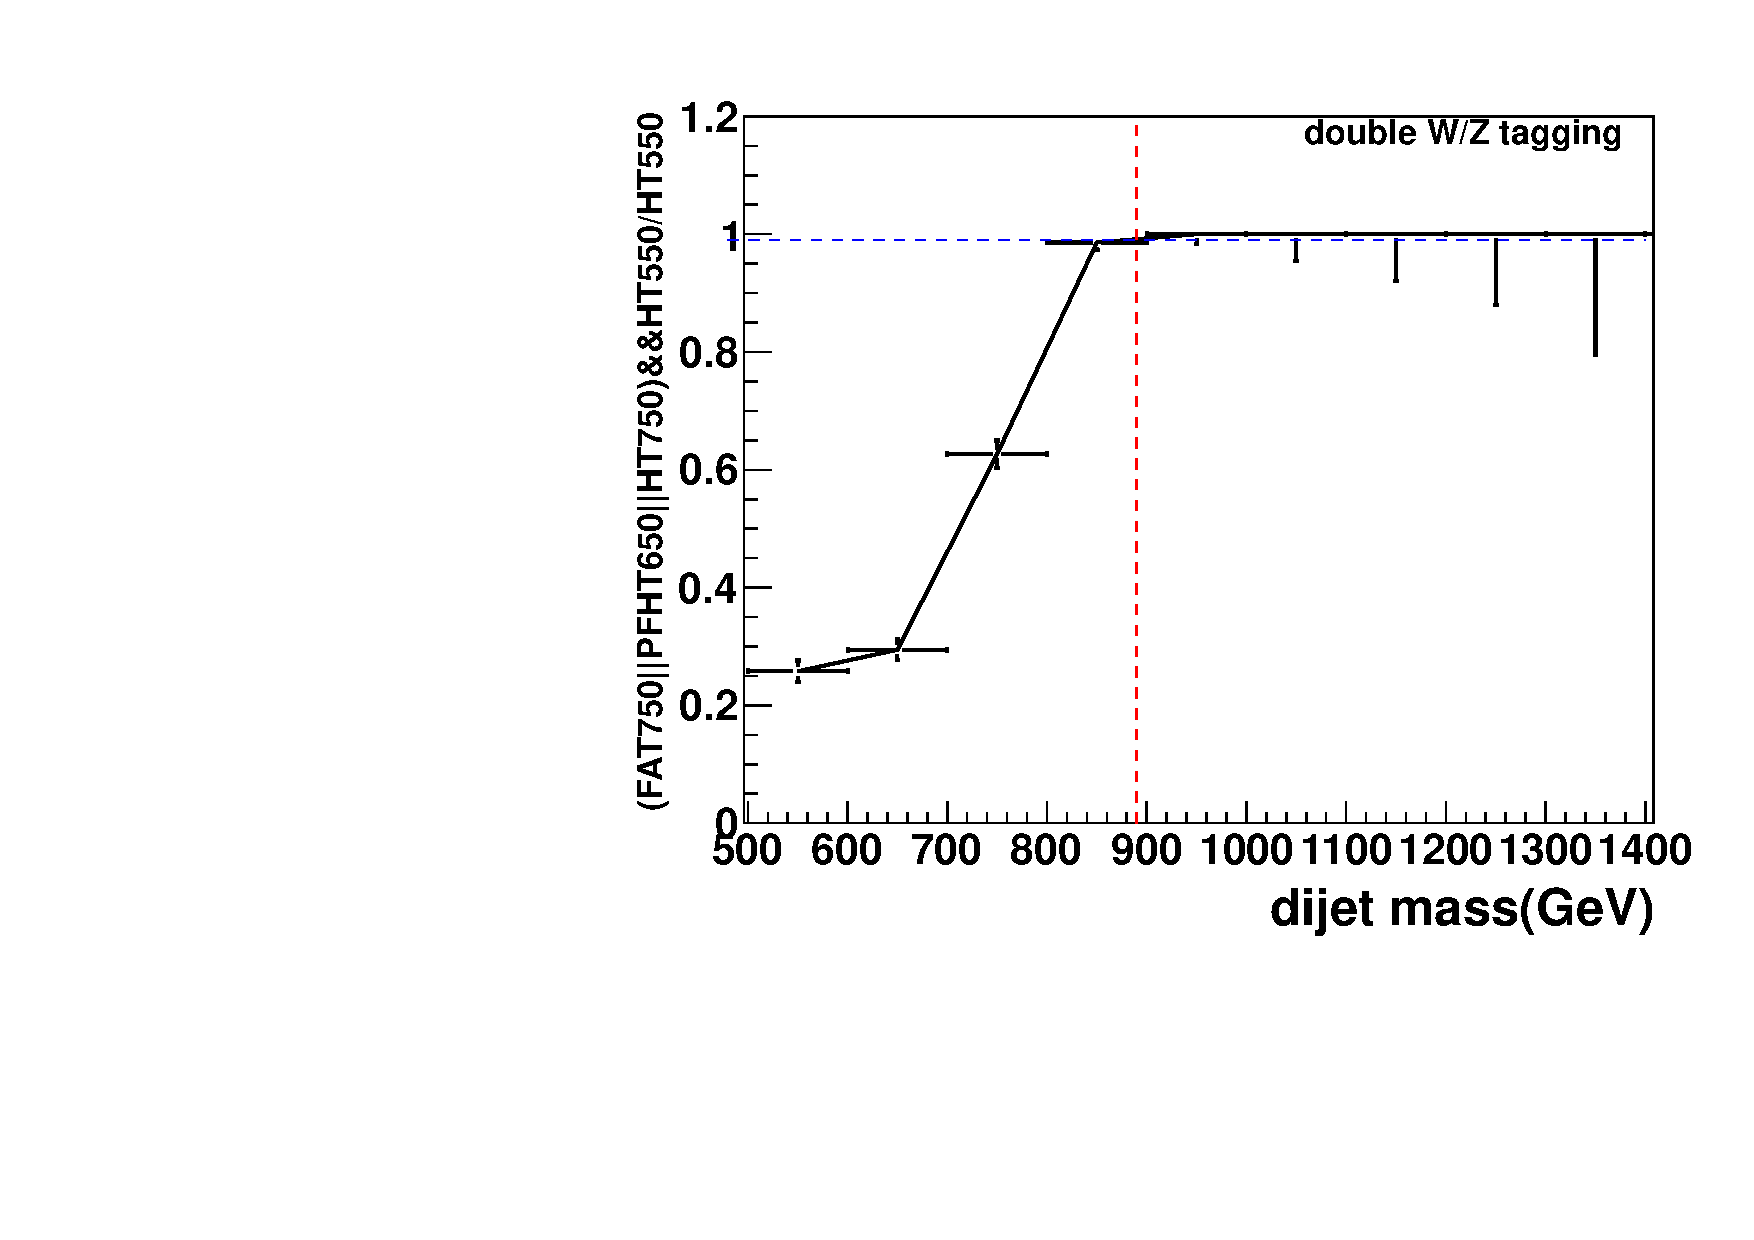
\includegraphics{EXO-12-024/figs/trigger-eff/Dataeff_doubletagging.pdf}} \\
\caption[Trigger efficiencies]{Trigger efficiency for double tagged data of FAT\_750$\parallel$HLT\_PF(NoPU)HT650$\parallel$HLT\_HT750 measured using data collected by lower threshold $H_T550$ trigger. The dash red line is positioned at $m_{jj}$ equal $890 GeV$, the blue line is at efficiency at 99$\%$. }
  \label{fig:trigger efficiencies part3}
\end{figure}


\clearpage














%\newpage
\section{Data and MC comparisons}
\label{sec:data-mc-comp}

In this section, we compare some kinematic features of the jets between QCD MC and data, which are
 shown in Fig~\ref{fig:mjjSingle}, \ref{fig:mjjDouble},\ref{fig:dySingle}, \ref{fig:dyDouble}, \ref{fig:dphiSingle}, 
\ref{fig:dphiDouble},\ref{fig:metSumPtSingle},
\ref{fig:Pt0Single}, \ref{fig:Pt0Double}, \ref{fig:Pt1Single}, \ref{fig:Pt1Double},
\ref{fig:Eta0Single}, \ref{fig:Eta0Double}, \ref{fig:Eta1Single}, \ref{fig:Eta1Double},
%\ref{fig:CA8Single},\ref{fig:CA8Double}
and \ref{fig:massNsub}.
Predictions from Pythia6 with Tune $Z2*$ and Herwig++ with Tune 23 are shown.
The comparison is shown in the exclusive dijet category, low and high purity,  single and double tagged events..
The distributions are shown after the event selection (in particular $|y| < 2.5$, $|\Delta\eta|<1.3$, $m_{jj} > 890  \GeVcc$) is applied.
The number of data events in each mass bin are shown in Table~\ref{table:eventnumbers}.
The MC is normalized to the number of data events in each category and the shapes are compared.


\begin{table}[htb]
%\begin{center}
\begin{tabular}{|p{3.0cm}|p{3.0cm}|p{3.0cm}|p{3.0cm}|p{3.0cm}|}
%\begin{tabular}{|c|c|c|c|c|}
\hline
lower mass bin border & low purity 1-tag events & high purity 1-tag events& low purity 2-tag events& high purity 2-tag events\\
\hline
890 & 165671 & 105892 & 7586 & 2544 \\ 
944 & 115622 & 72007 & 4950 & 1673 \\ 
1000 & 80537 & 48930 & 3311 & 1005 \\ 
1058 & 56423 & 33398 & 2159 & 658 \\ 
1118 & 39817 & 23086 & 1407 & 427 \\ 
1181 & 27651 & 15817 & 962 & 302 \\ 
1246 & 19531 & 10741 & 647 & 175 \\ 
1313 & 13617 & 7477 & 434 & 135 \\ 
1383 & 9880 & 5128 & 272 & 75 \\ 
1455 & 6992 & 3578 & 195 & 49 \\ 
1530 & 4939 & 2525 & 138 & 25 \\ 
1607 & 3443 & 1658 & 86 & 24 \\ 
1687 & 2454 & 1160 & 52 & 10 \\ 
1770 & 1744 & 815 & 42 & 9 \\ 
1856 & 1193 & 547 & 35 & 6 \\ 
1945 & 881 & 389 & 21 & 4 \\ 
2037 & 643 & 230 & 12 & 3 \\ 
2132 & 402 & 167 & 8 & 3 \\ 
2231 & 287 & 99 & 5 & 1 \\ 
2332 & 193 & 86 & 3 &  \\ 
2438 & 138 & 57 & 1 &  \\ 
2546 & 87 & 28 & 0 &  \\ 
2659 & 60 & 13 & 2 &  \\ 
2775 & 48 & 11 &  &  \\ 
2895 & 38 & 5 &  &  \\ 
3019 & 14 & 4 &  &  \\ 
3147 & 17 & 3 &  &  \\ 
3279 & 4 & 1 &  &  \\ 
3416 & 4 & 0 &  &  \\ 
3558 & 4 & 1 &  &  \\ 
3704 &  & 1 &  &  \\ 
3854 &  &  &  &  \\ 
4010 &  &  &  &  \\ 
\hline
\end{tabular}
\caption{Number of events in each mass bin exclusive, with 1 W/Z-tag and  2 W/Z-tags required in low
purity and high purity categories.}
\label{table:eventnumbers}
\end{table}



\newpage


\begin{figure}[htb]
\centering
\begin{tabular}{cc}
     \resizebox{0.5\linewidth}{!}{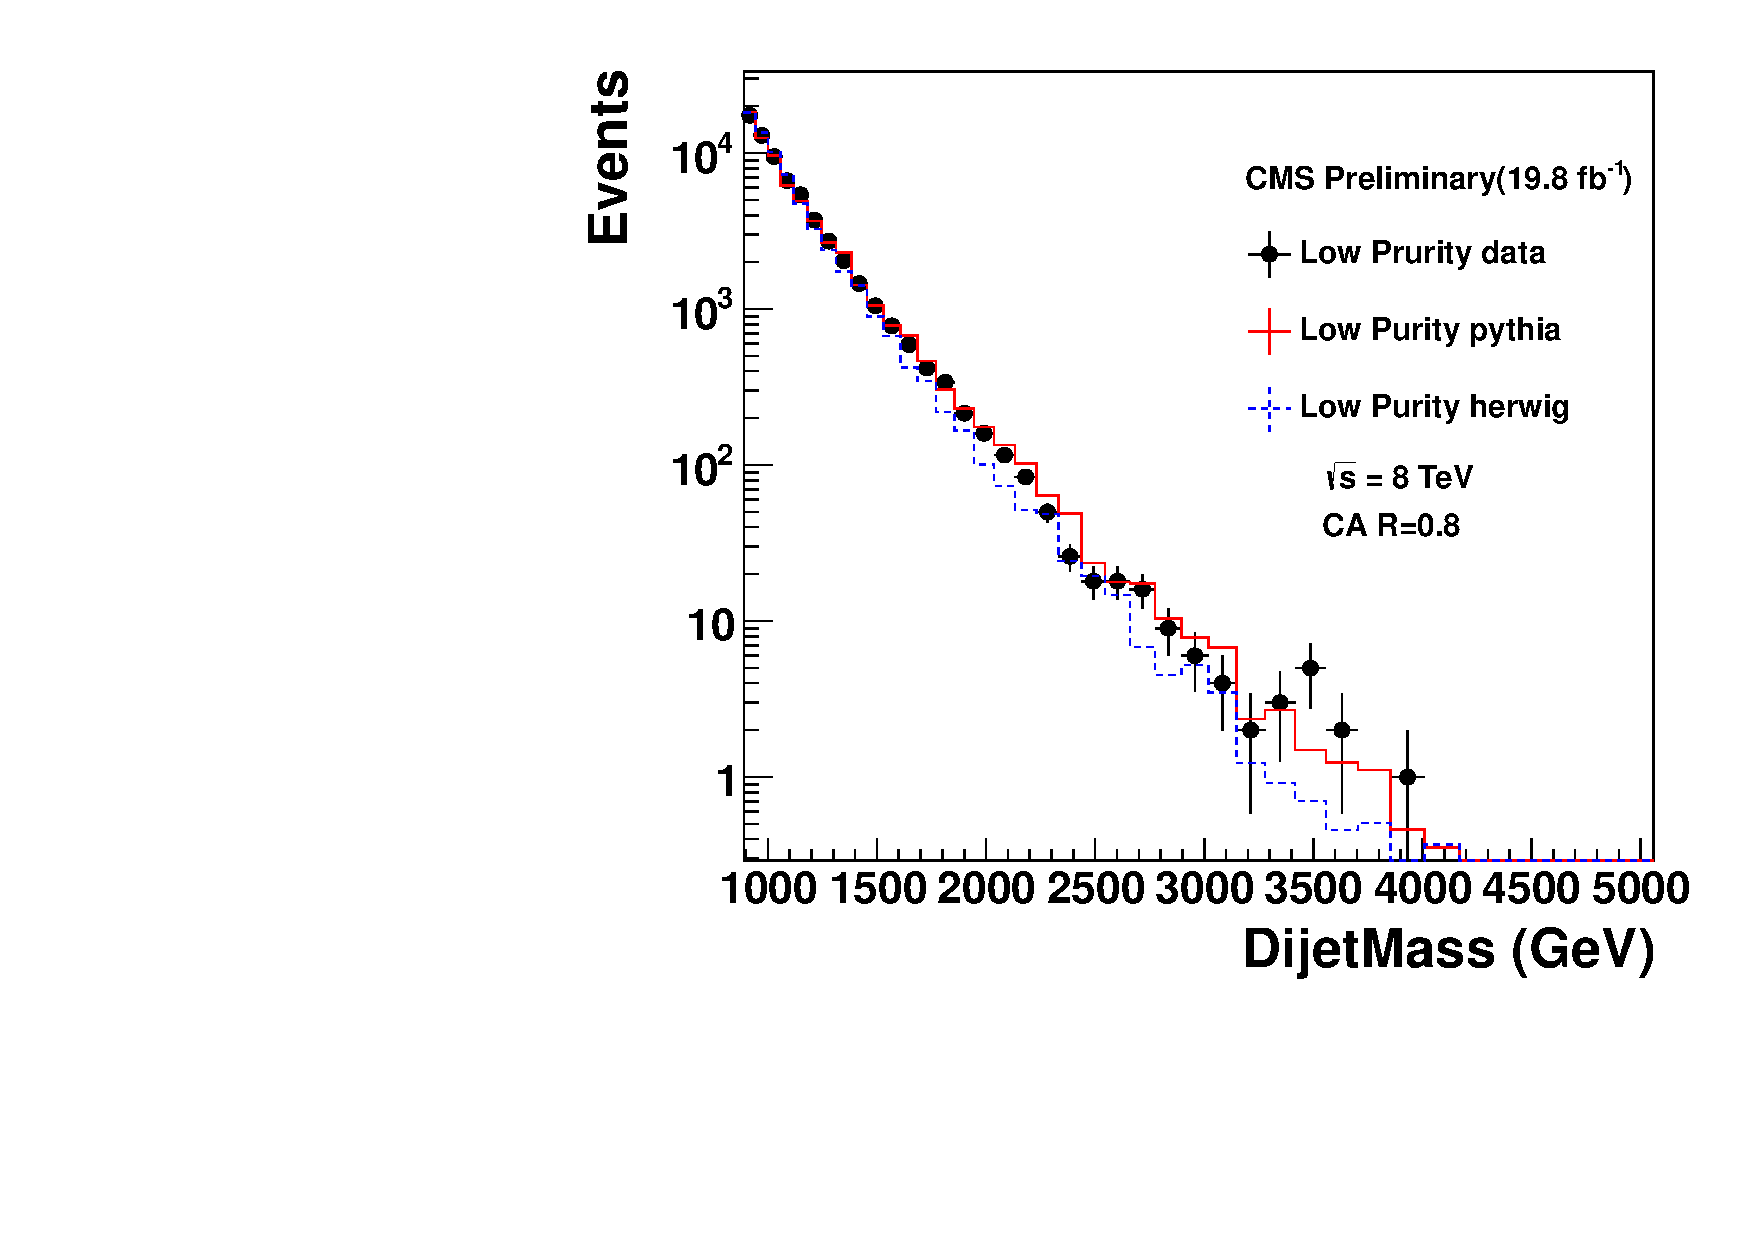
\includegraphics{figs/Data-MC-comparisons/DijetMass-qVLowP.pdf}} &
     \resizebox{0.5\linewidth}{!}{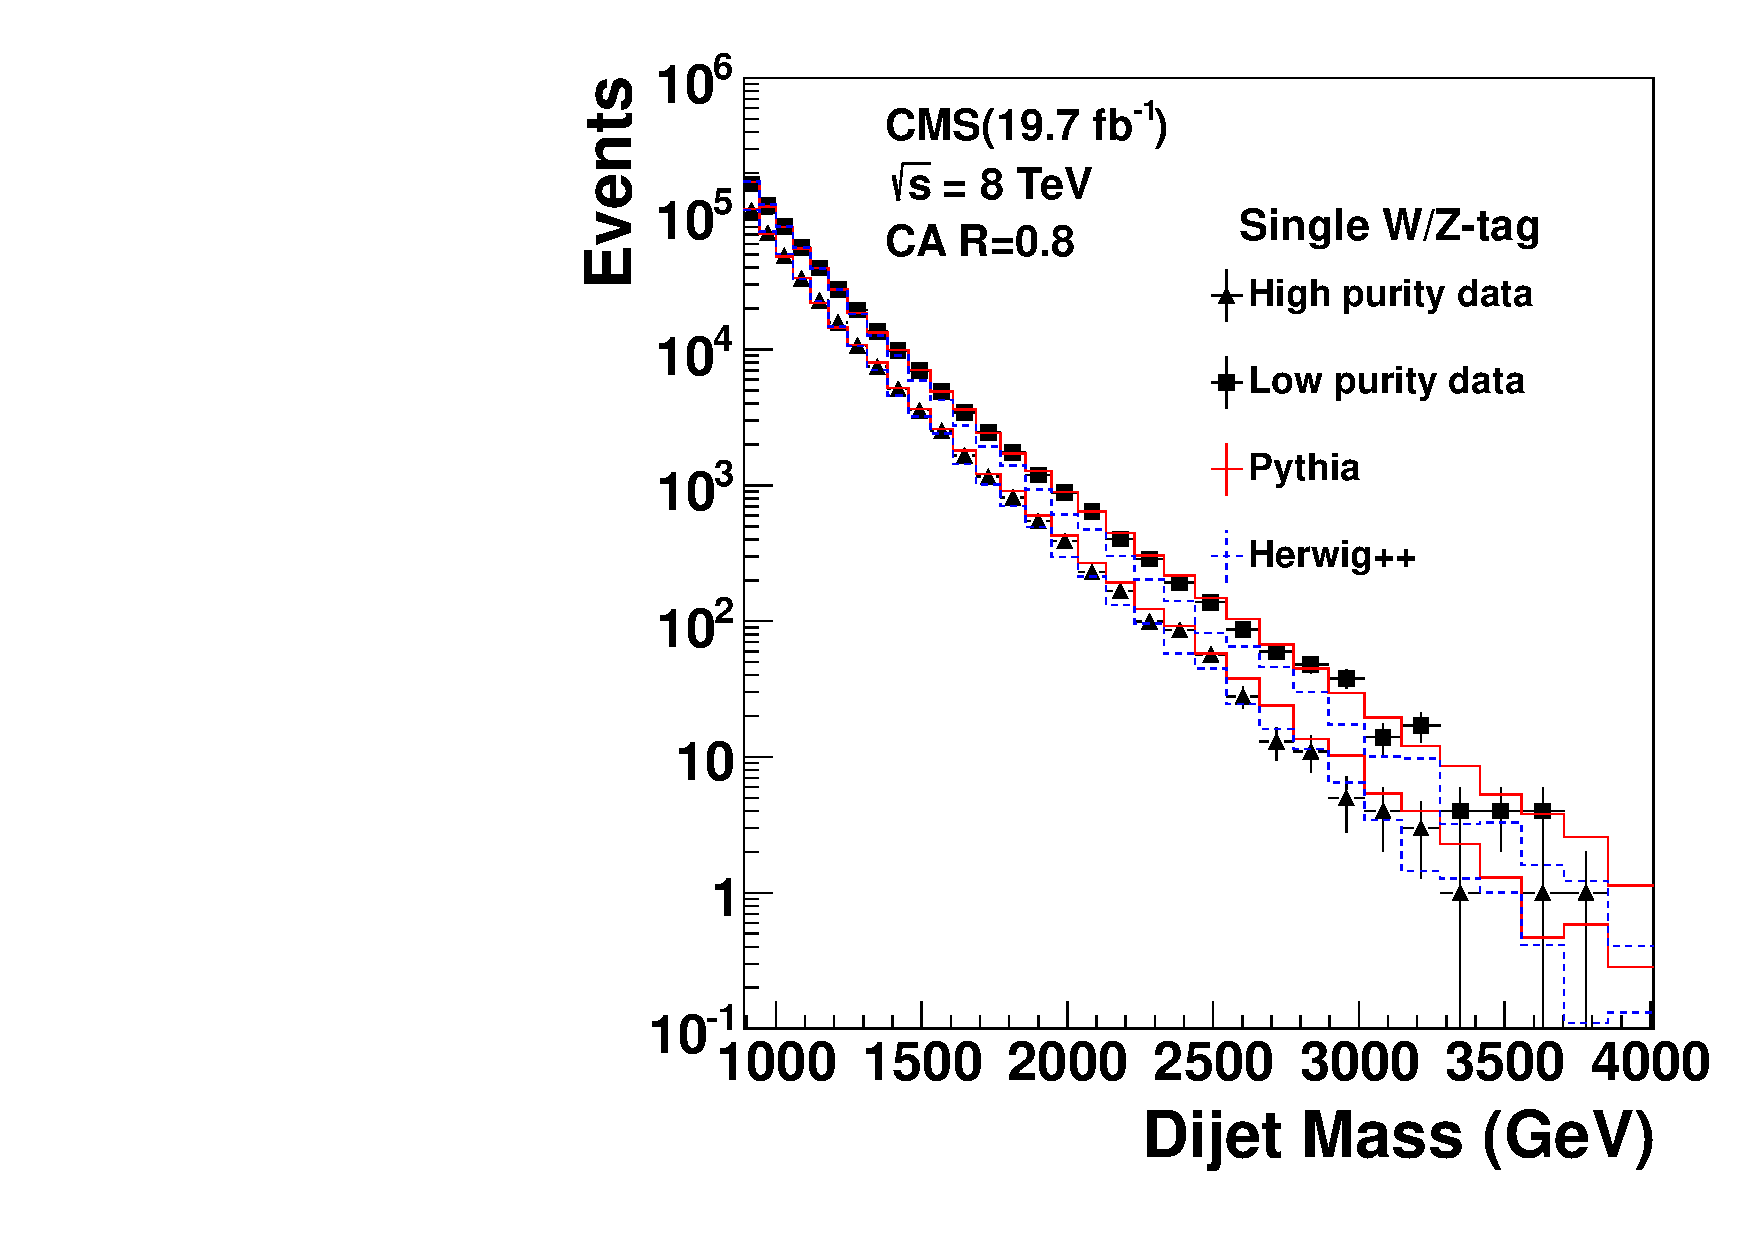
\includegraphics{figs/Data-MC-comparisons/DijetMass-qVMiumHigh.pdf}} \\
\end{tabular}
  \caption[Invariant Mass Single]{Comparisons between data and Monte Carlo
           for invariant mass of the two leading jets of low purity (left) and low-high purity (right) 1-tagged events.
           The MC is normalized to the number of data events in each category.
           }
  \label{fig:mjjSingle}
\end{figure}

\begin{figure}[htb]
\centering
\begin{tabular}{cc}
     \resizebox{0.5\linewidth}{!}{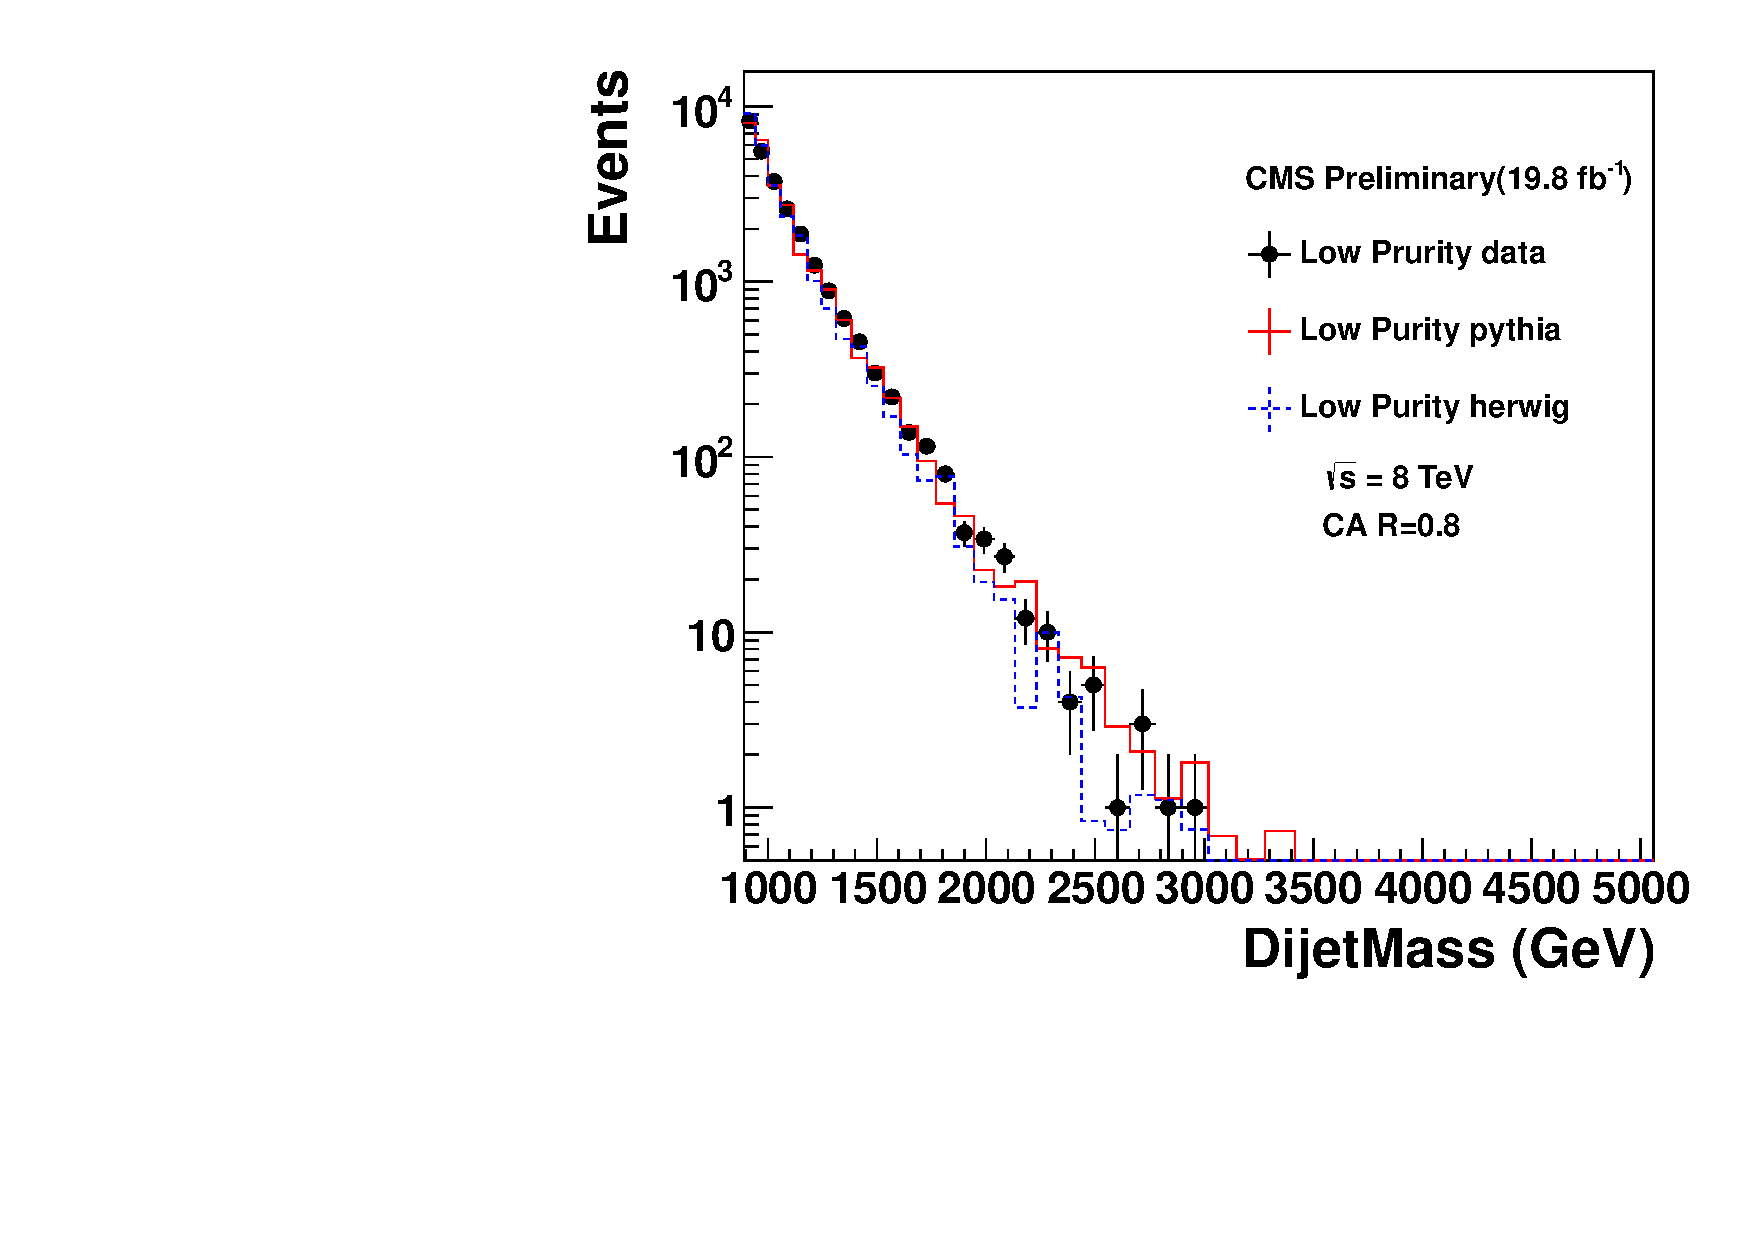
\includegraphics{figs/Data-MC-comparisons/DijetMass-VVLowP.pdf}} &
     \resizebox{0.5\linewidth}{!}{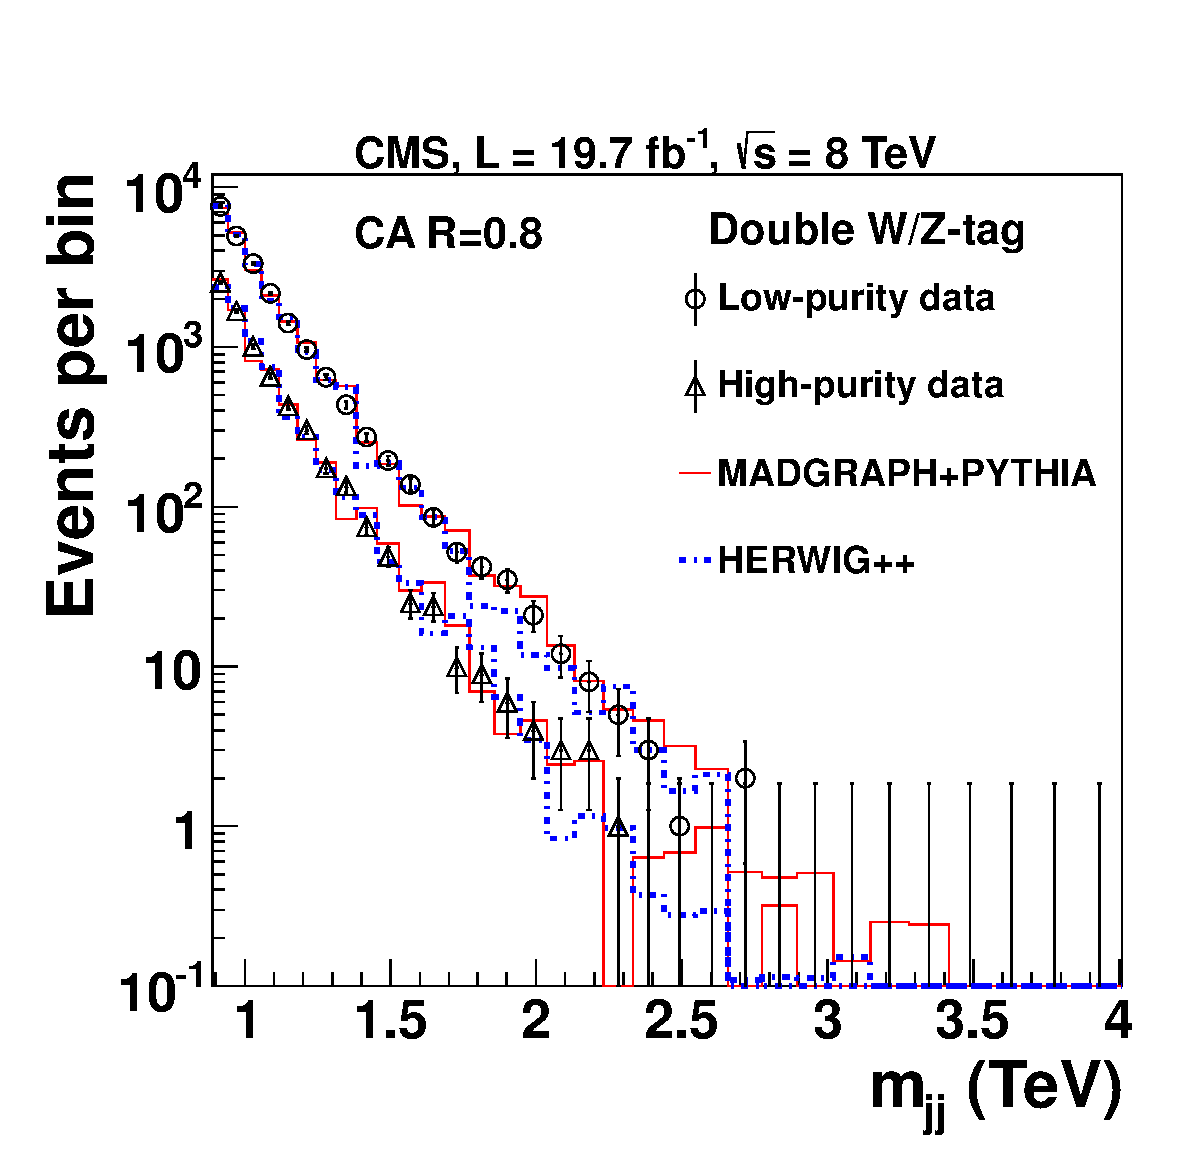
\includegraphics{figs/Data-MC-comparisons/DijetMass-VVMiumHigh.pdf}} \\
\end{tabular}
  \caption[Invariant Mass Double]{Comparisons between data and Monte Carlo
           for invariant mass of the two leading jets of low purity (left) and low-high purity (right) 2-tagged events.
           The MC is normalized to the number of data events in each category.
           }
  \label{fig:mjjDouble}
\end{figure}

\newpage
\begin{figure}[htb]
\centering
\begin{tabular}{cc}
     \resizebox{0.5\linewidth}{!}{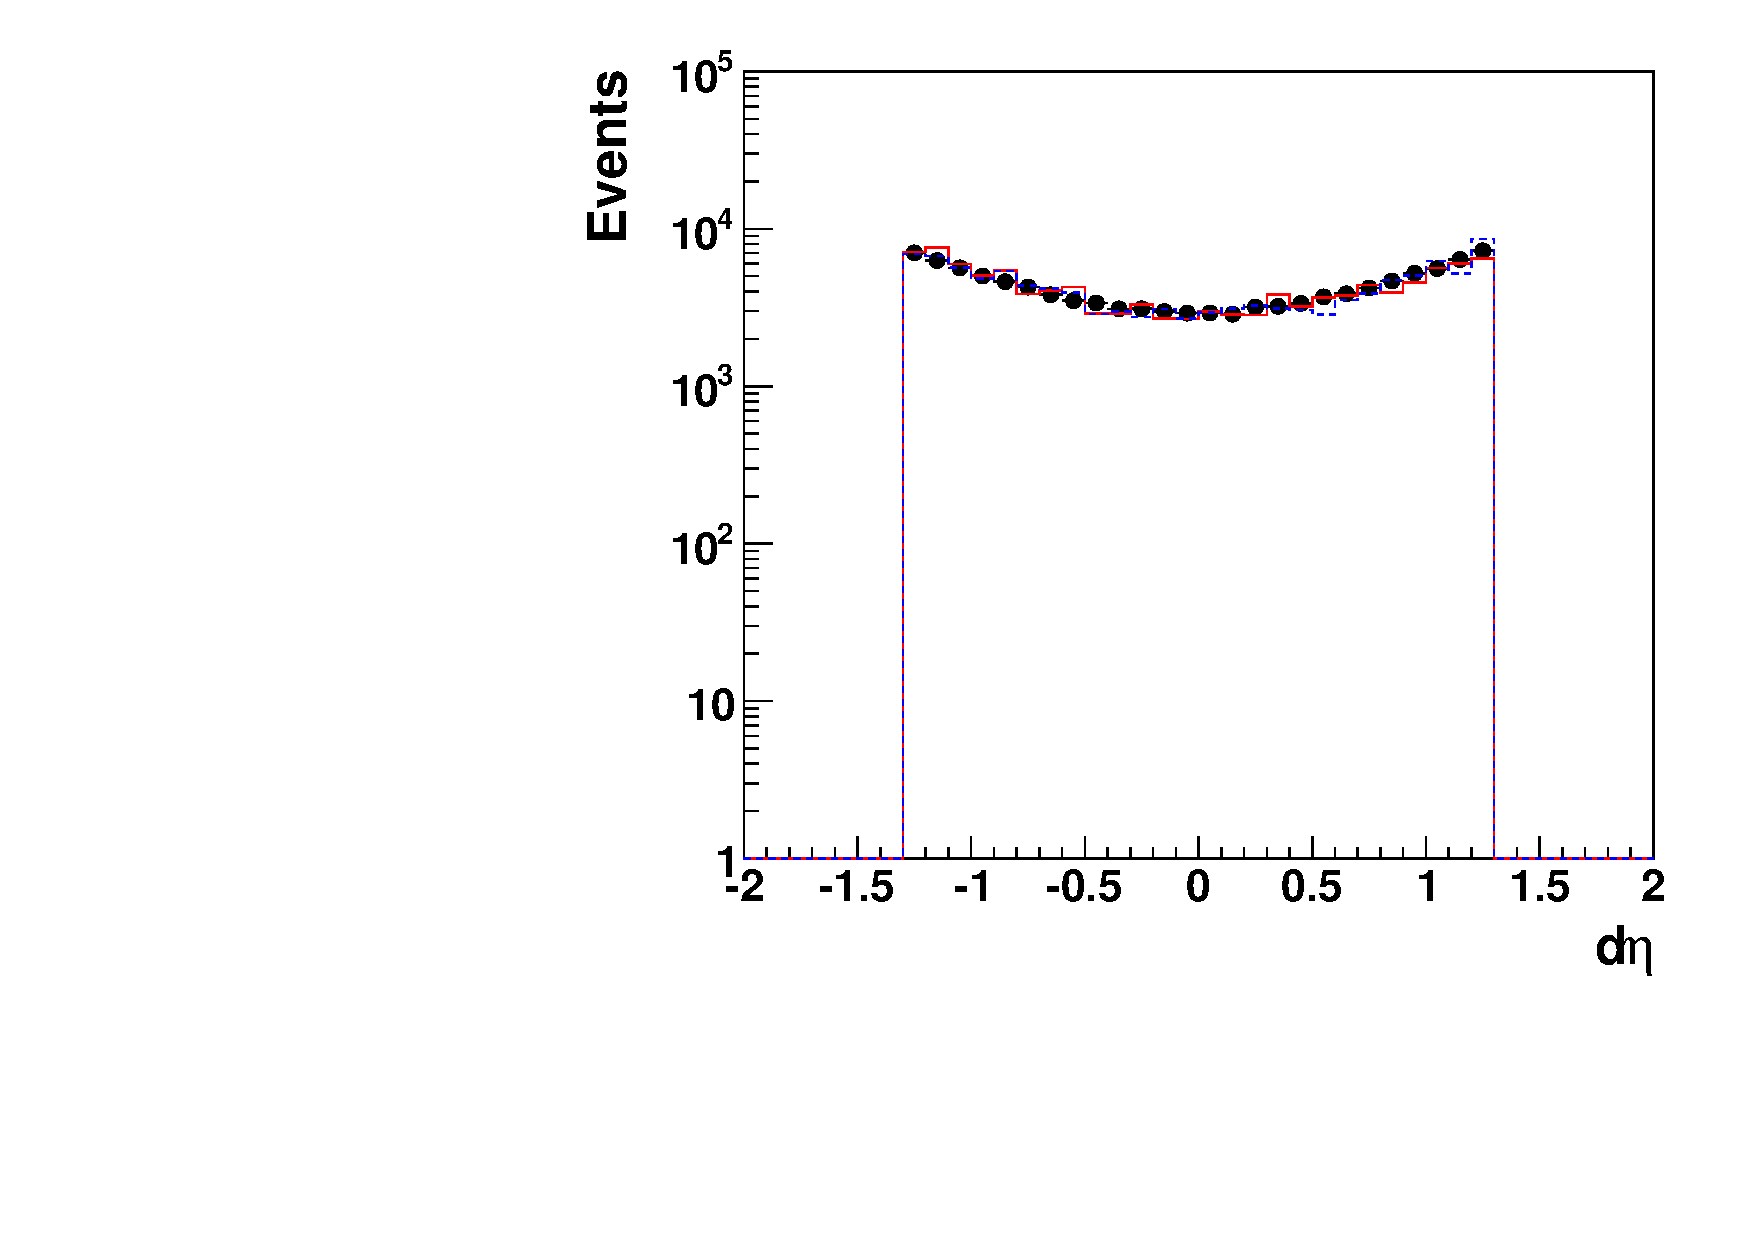
\includegraphics{figs/Data-MC-comparisons/Deta-qVLowP.pdf}} &
     \resizebox{0.5\linewidth}{!}{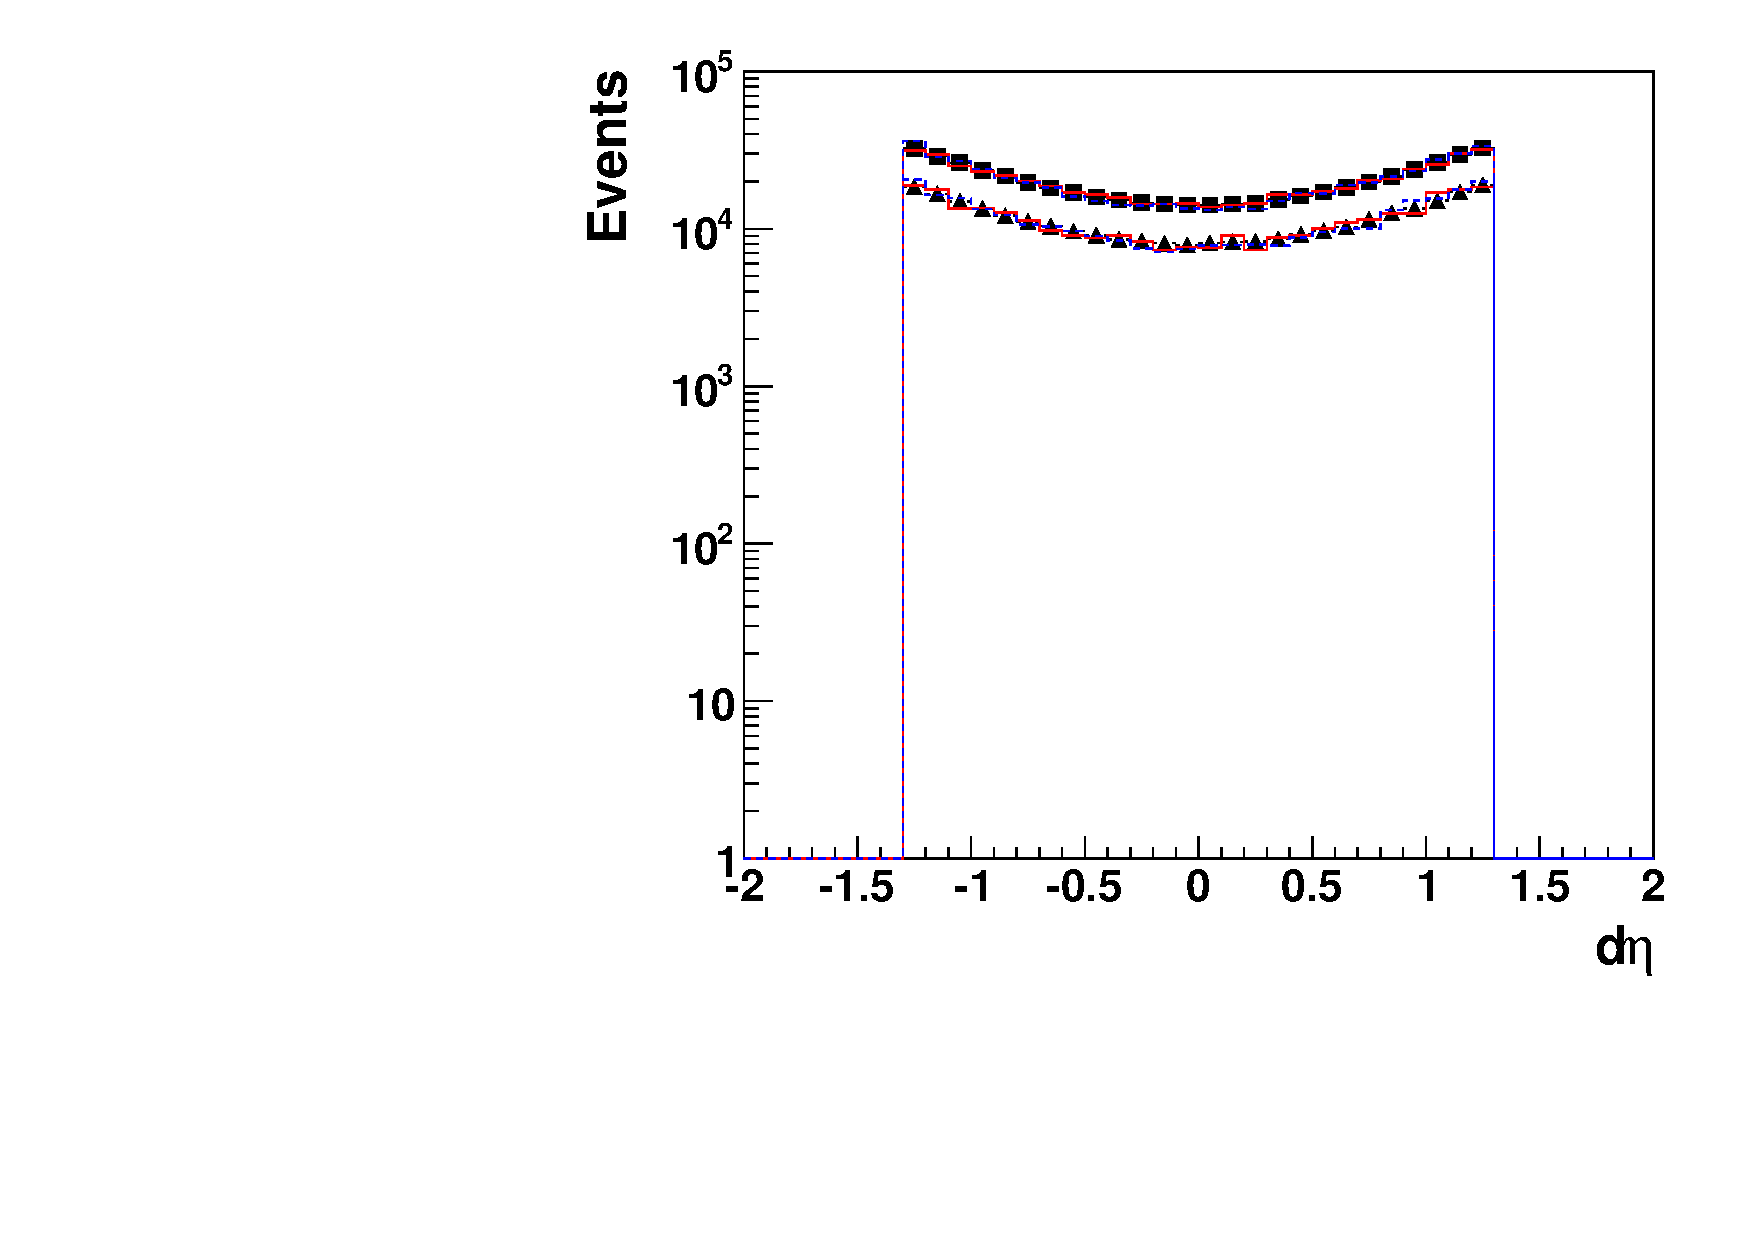
\includegraphics{figs/Data-MC-comparisons/Deta-qVMiumHigh.pdf}} \\
\end{tabular}
  \caption[Delta Eta Single]{Comparisons between data and Monte Carlo
                    for $\Delta\eta$ of the two leading jets of low purity (left) and low-high purity (right) 1-tagged events.
	   The MC is normalized to the number of data events in each category. }
  \label{fig:dySingle}
\end{figure}

\begin{figure}[htb]
\centering
\begin{tabular}{cc}
     \resizebox{0.5\linewidth}{!}{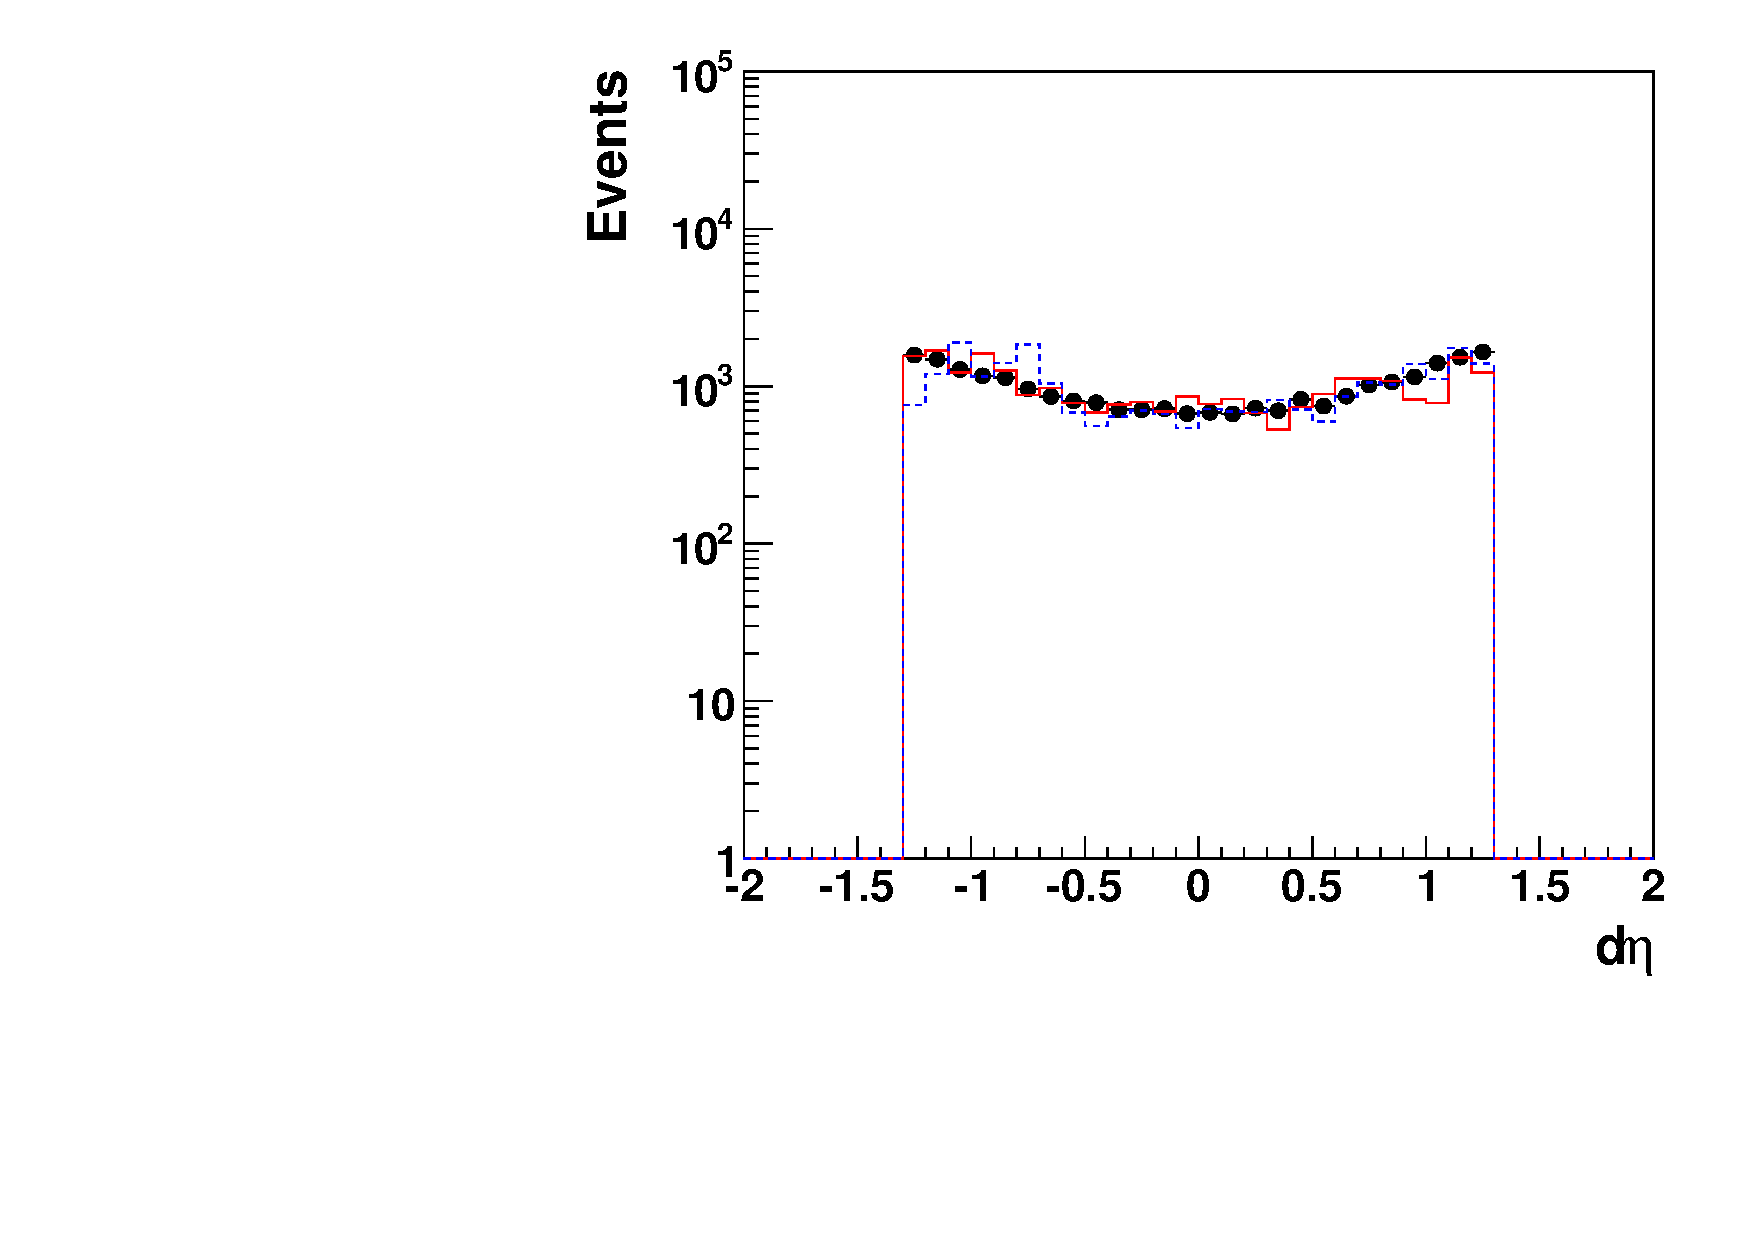
\includegraphics{figs/Data-MC-comparisons/Deta-VVLowP.pdf}} &
     \resizebox{0.5\linewidth}{!}{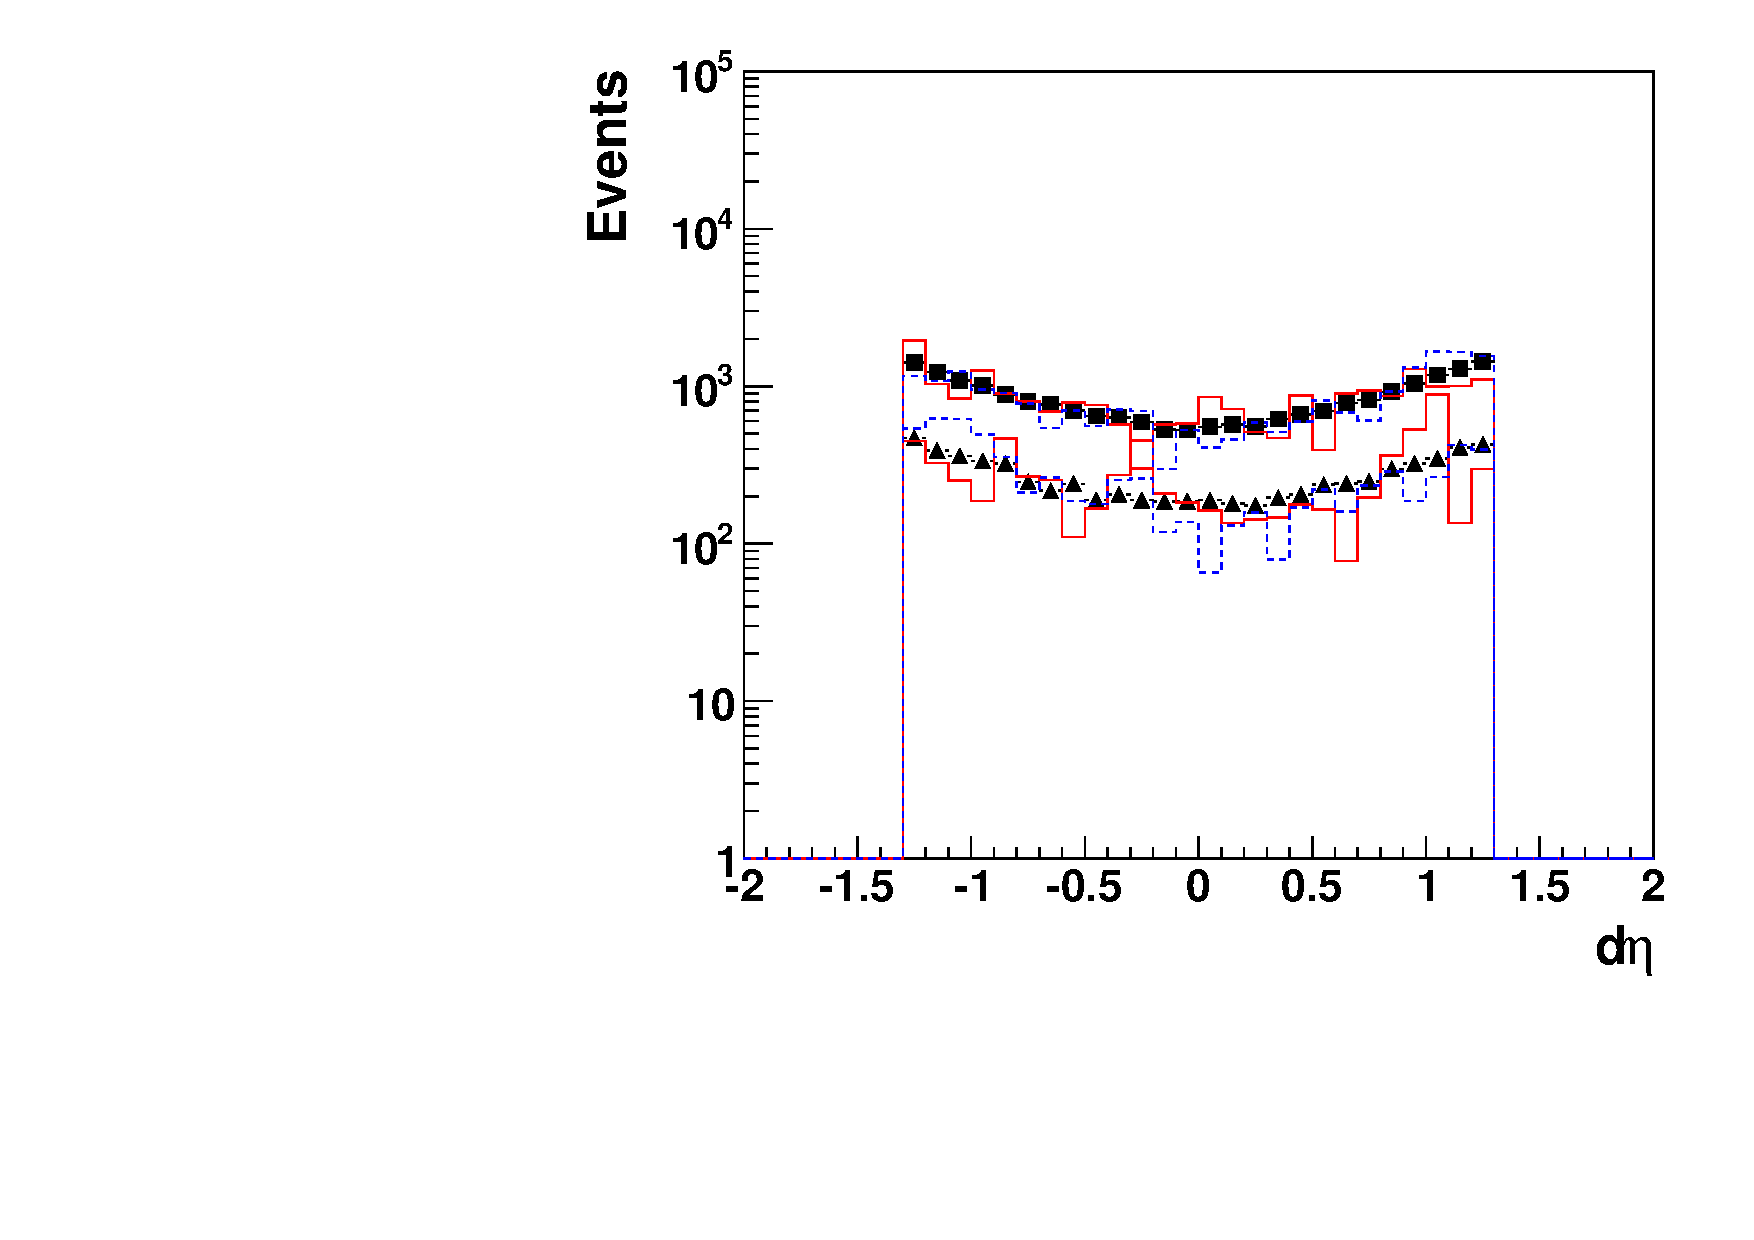
\includegraphics{figs/Data-MC-comparisons/Deta-VVMiumHigh.pdf}} \\
\end{tabular}
  \caption[Delta Eta Double]{Comparisons between data and Monte Carlo
                     for $\Delta\eta$ of the two leading jets of low purity (left) and low-high purity (right) 2-tagged events. The MC is normalized to the number of data events in each category. }
  \label{fig:dyDouble}
\end{figure}


\newpage
\begin{figure}[htb]
\centering
\begin{tabular}{cc}
     \resizebox{0.5\linewidth}{!}{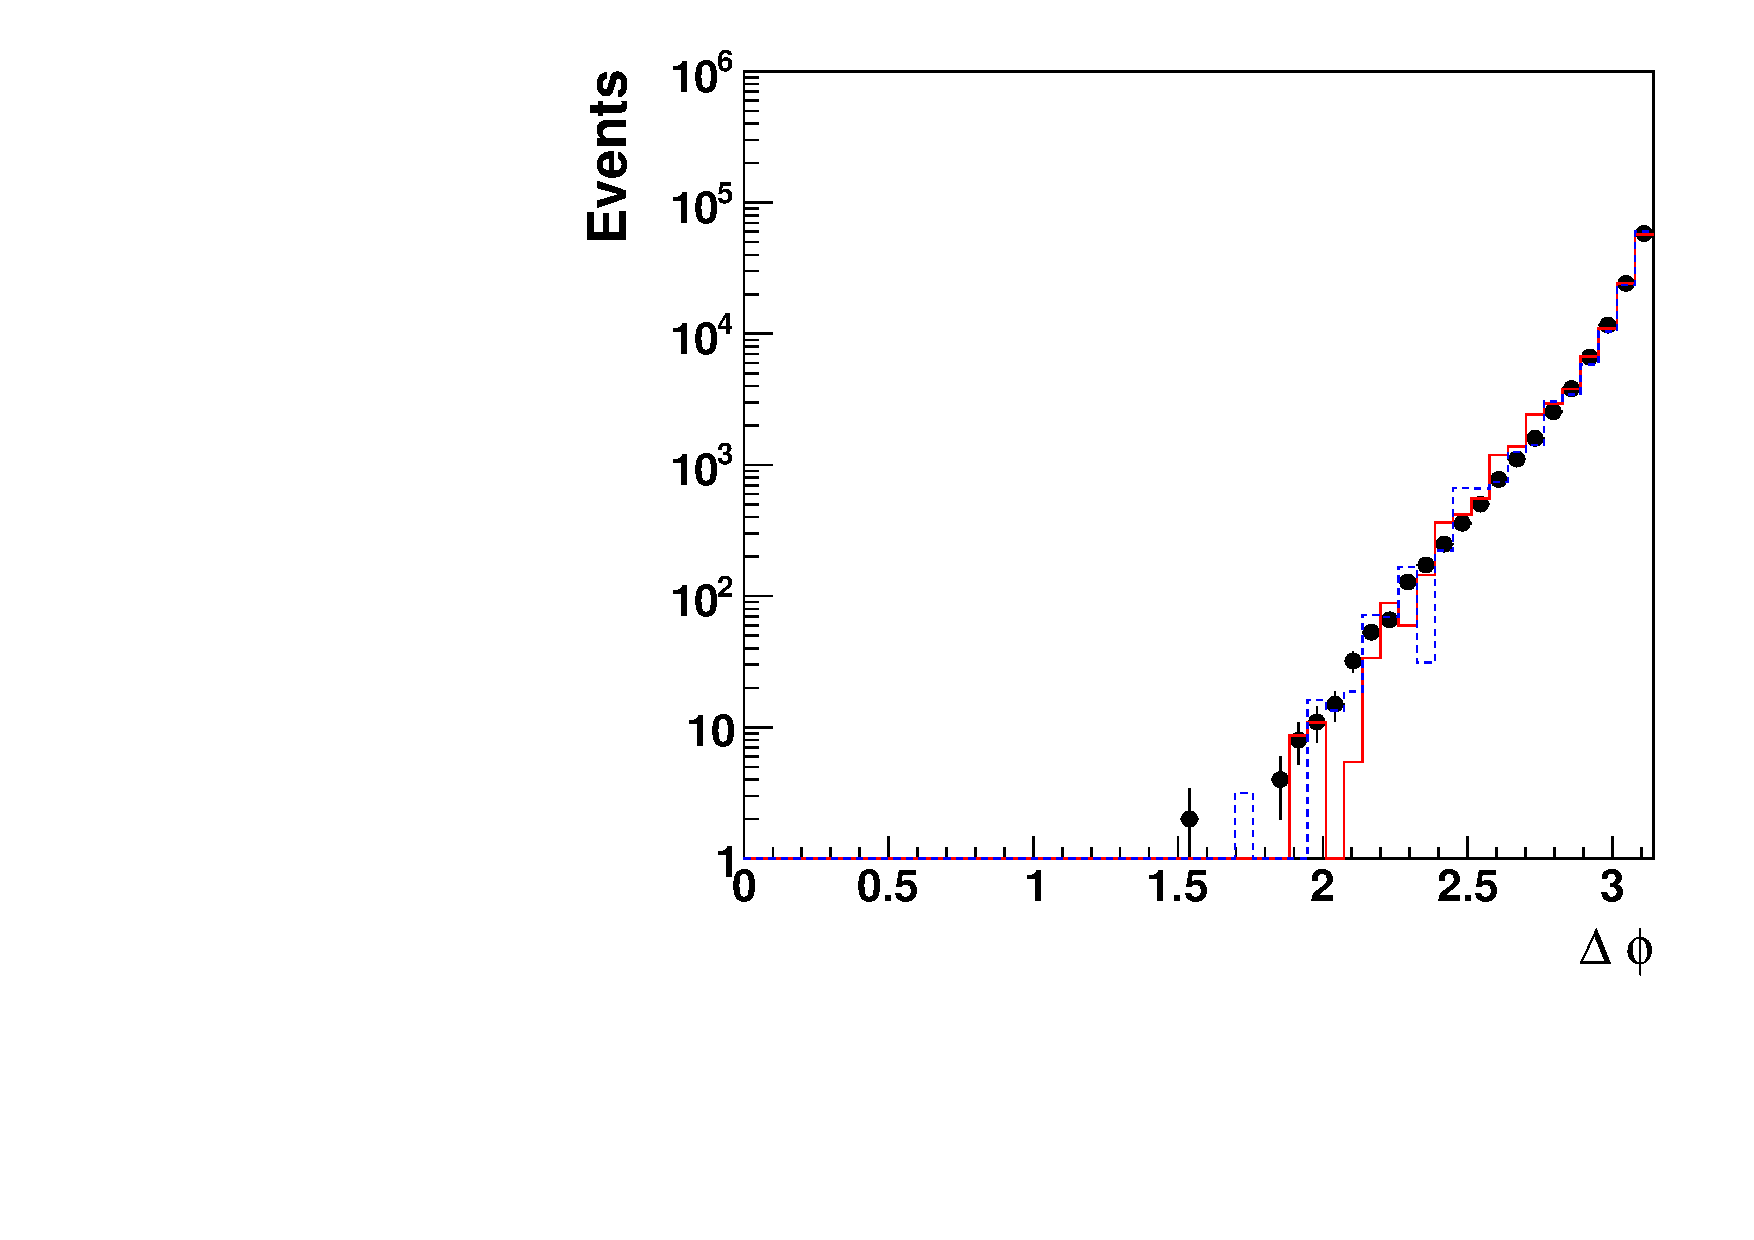
\includegraphics{figs/Data-MC-comparisons/Dphi-qVLowP.pdf}} &
     \resizebox{0.5\linewidth}{!}{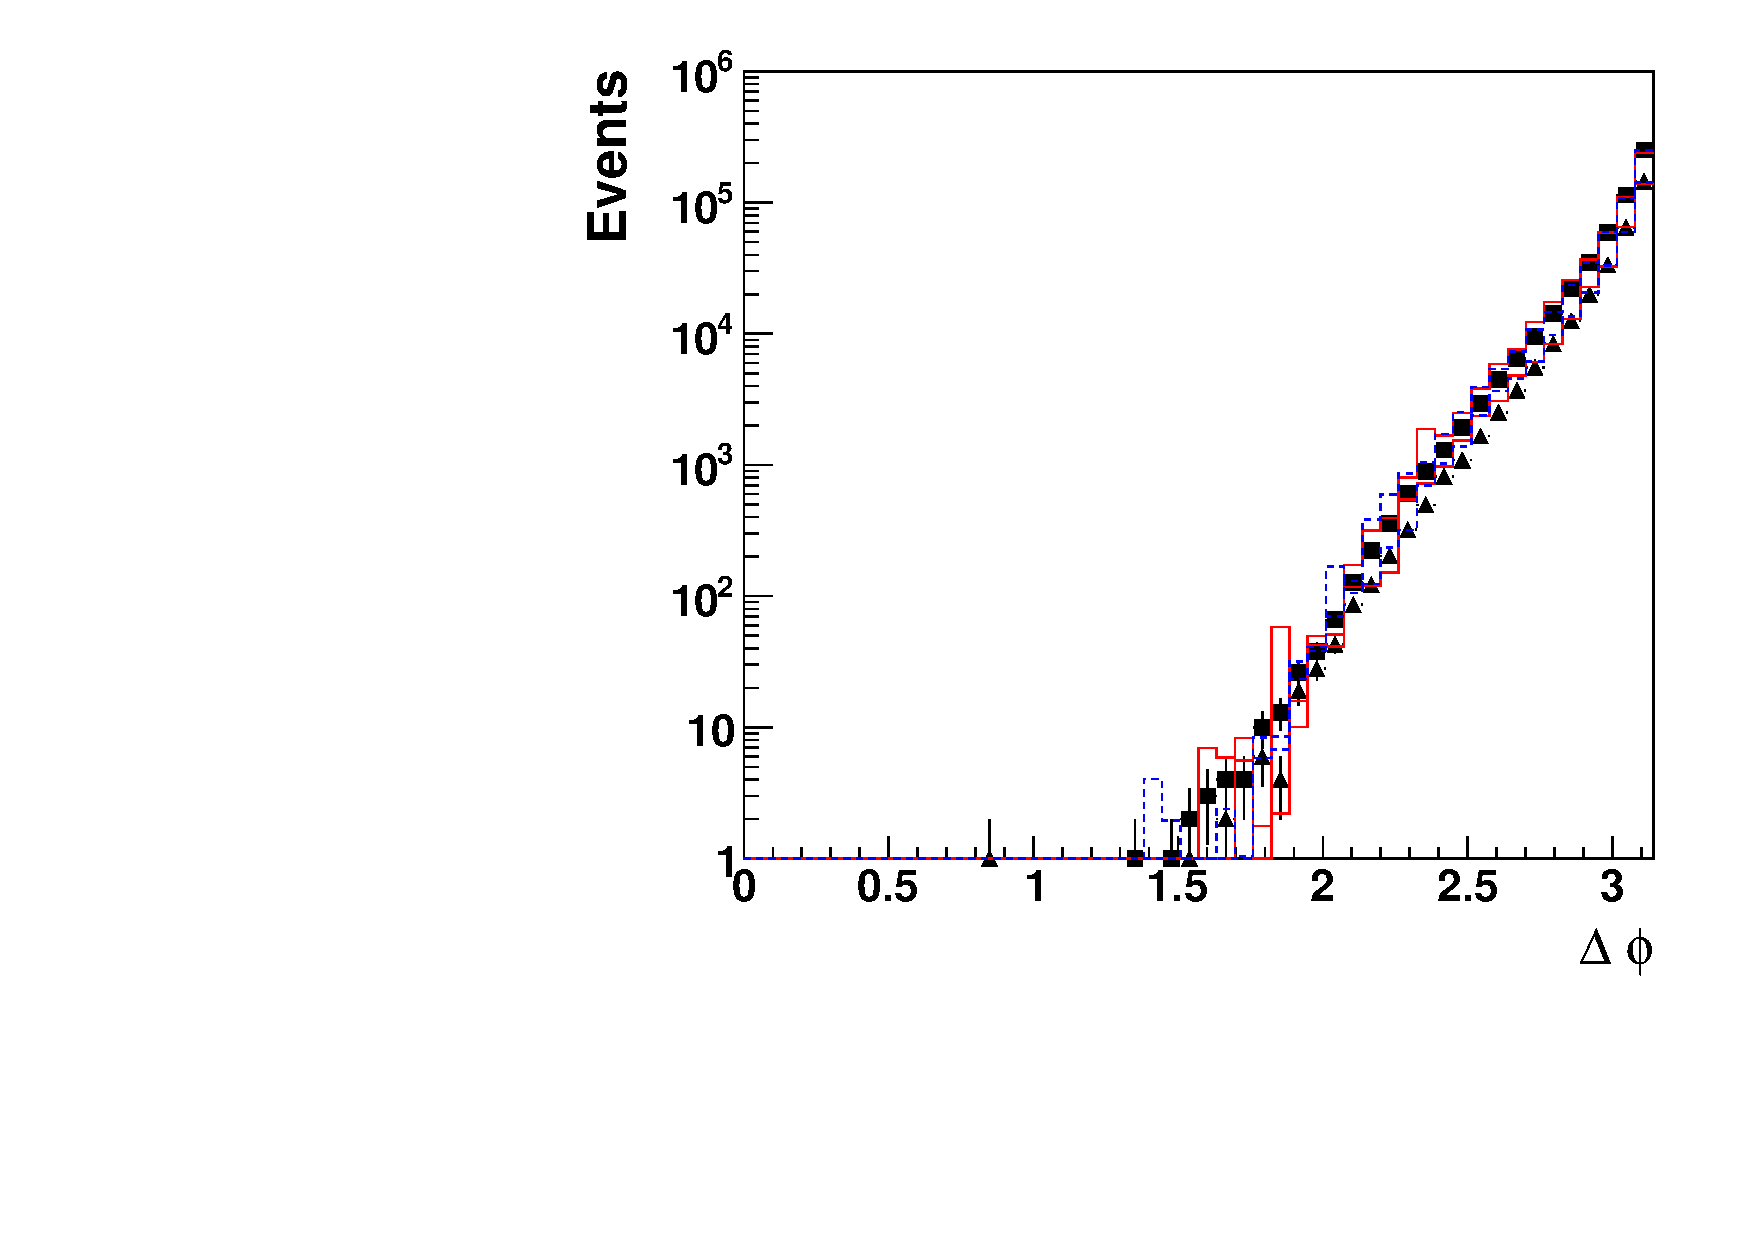
\includegraphics{figs/Data-MC-comparisons/Dphi-qVMiumHigh.pdf}} \\
\end{tabular}
  \caption[Delta Eta Single]{Comparisons between data and Monte Carlo
                    for $\Delta\phi$ of the two leading jets of low purity (left) and low-high purity (right) 1-tagged events.
	   The MC is normalized to the number of data events in each category. }
  \label{fig:dphiSingle}
\end{figure}

\begin{figure}[htb]
\centering
\begin{tabular}{cc}
     \resizebox{0.5\linewidth}{!}{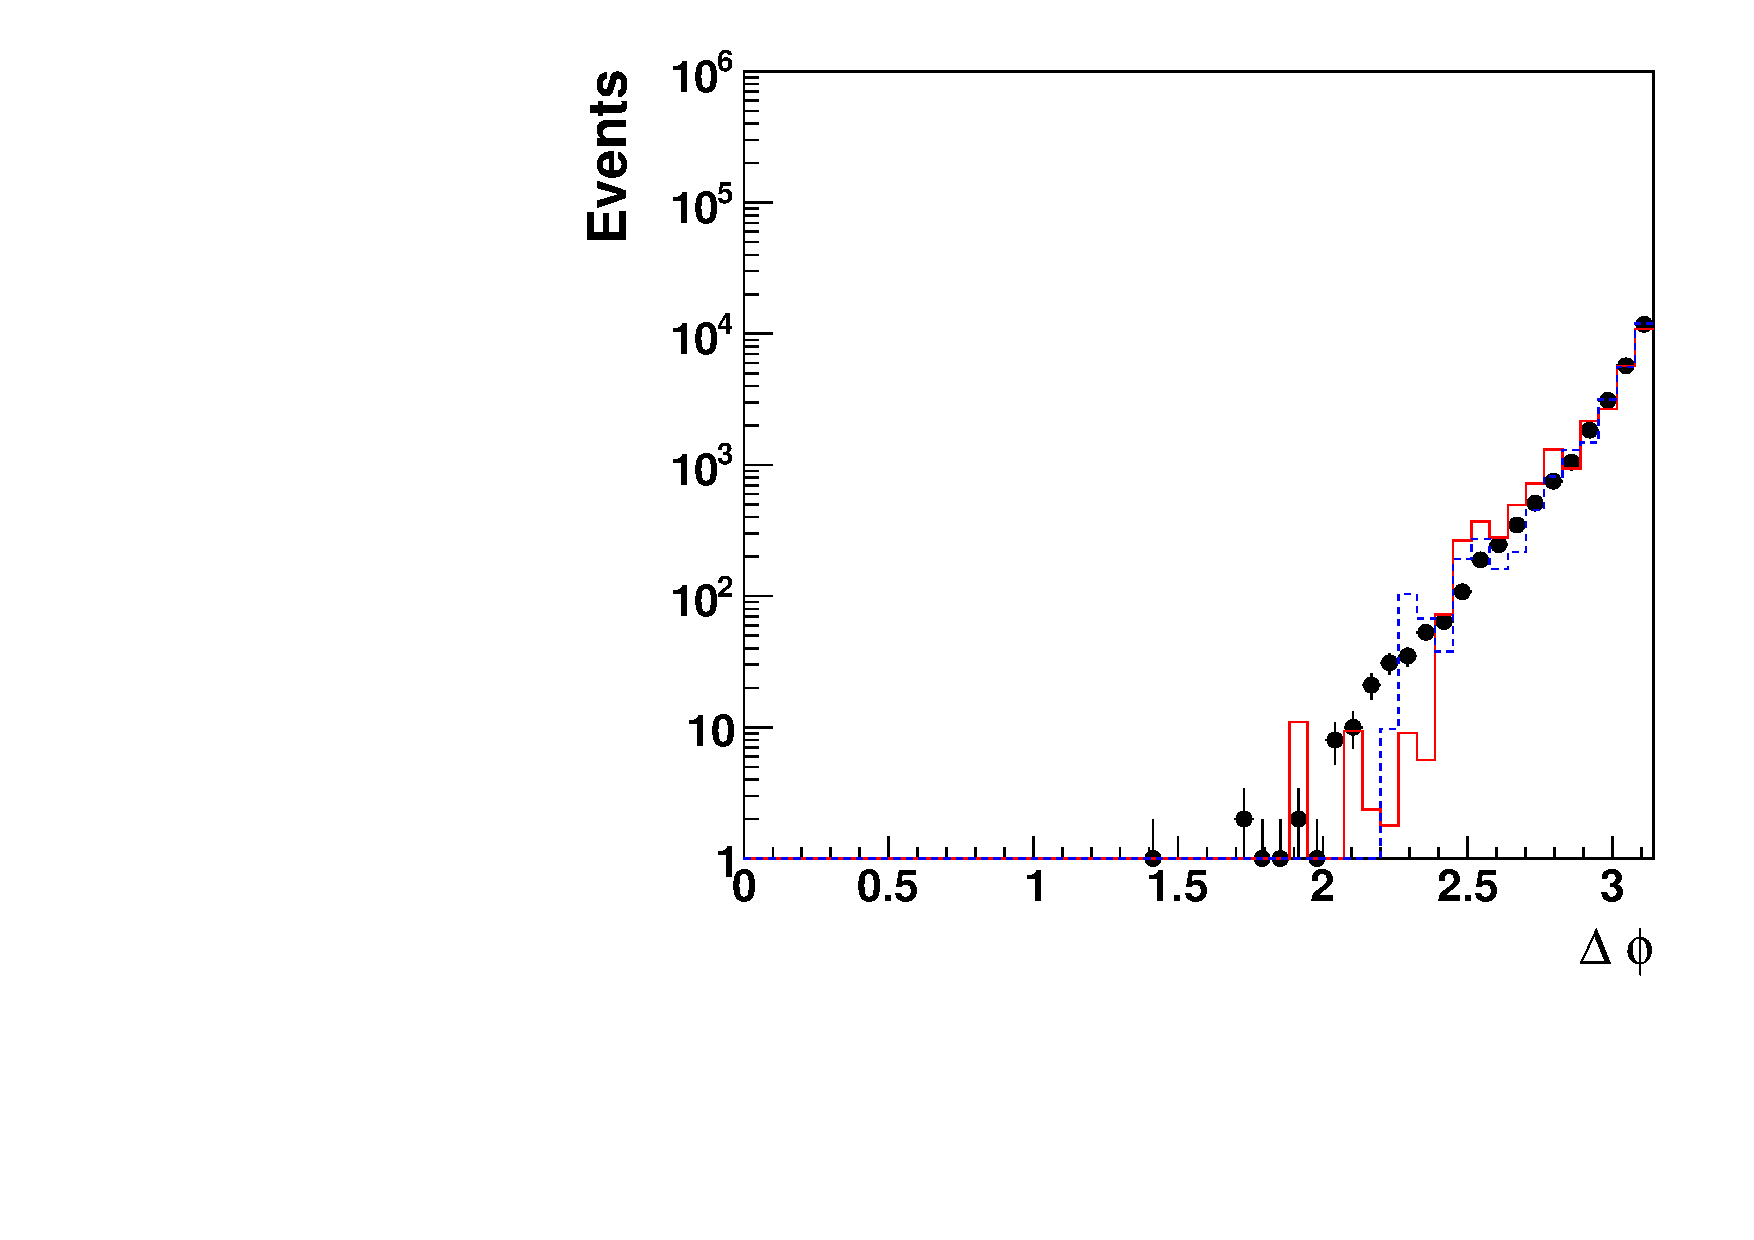
\includegraphics{figs/Data-MC-comparisons/Dphi-VVLowP.pdf}} &
     \resizebox{0.5\linewidth}{!}{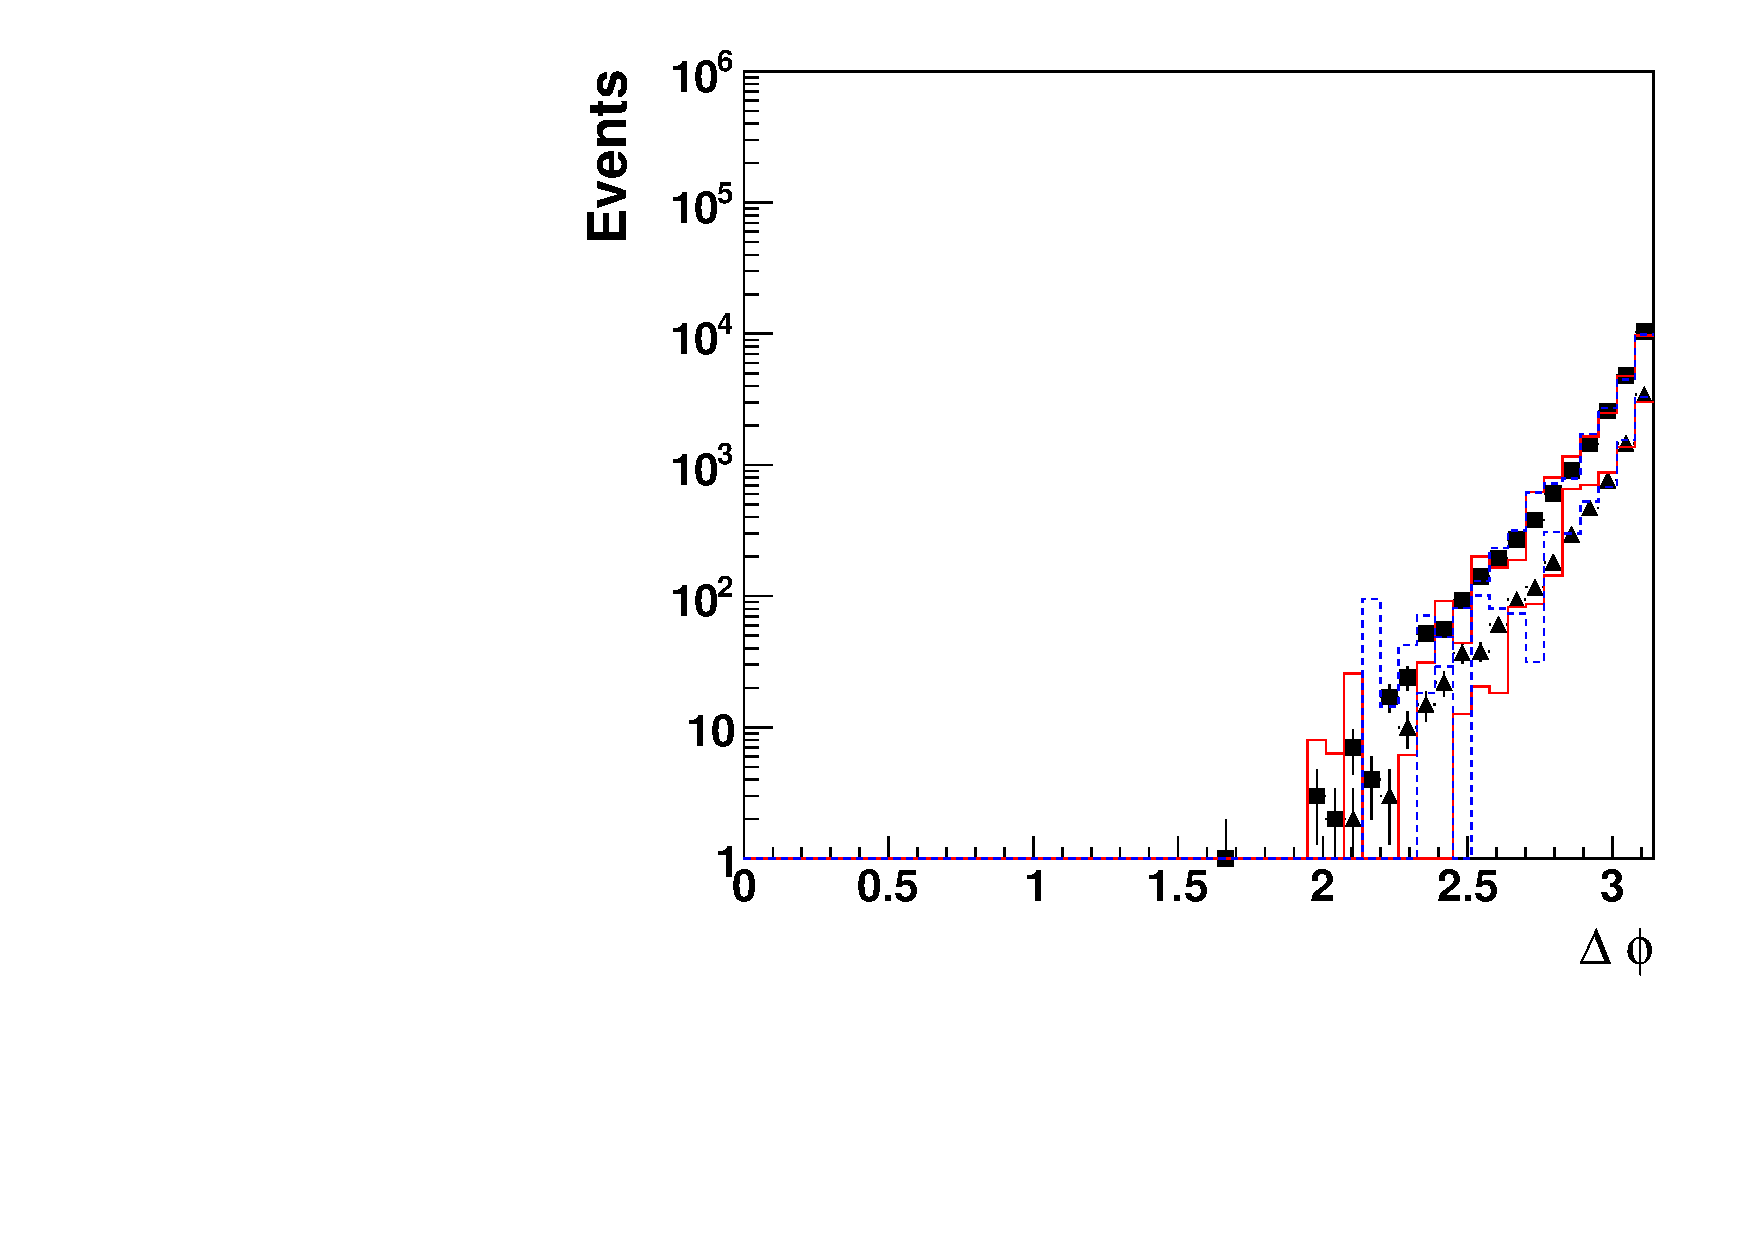
\includegraphics{figs/Data-MC-comparisons/Dphi-VVMiumHigh.pdf}} \\
\end{tabular}
  \caption[Delta Eta Double]{Comparisons between data and Monte Carlo
                     for $\Delta\phi$ of the two leading jets of low purity (left) and low-high purity (right) 2-tagged events. The MC is normalized to the number of data events in each category. }
  \label{fig:dphiDouble}
\end{figure}

\newpage

\begin{figure}[htb]
\centering
\begin{tabular}{cc}
     \resizebox{0.5\linewidth}{!}{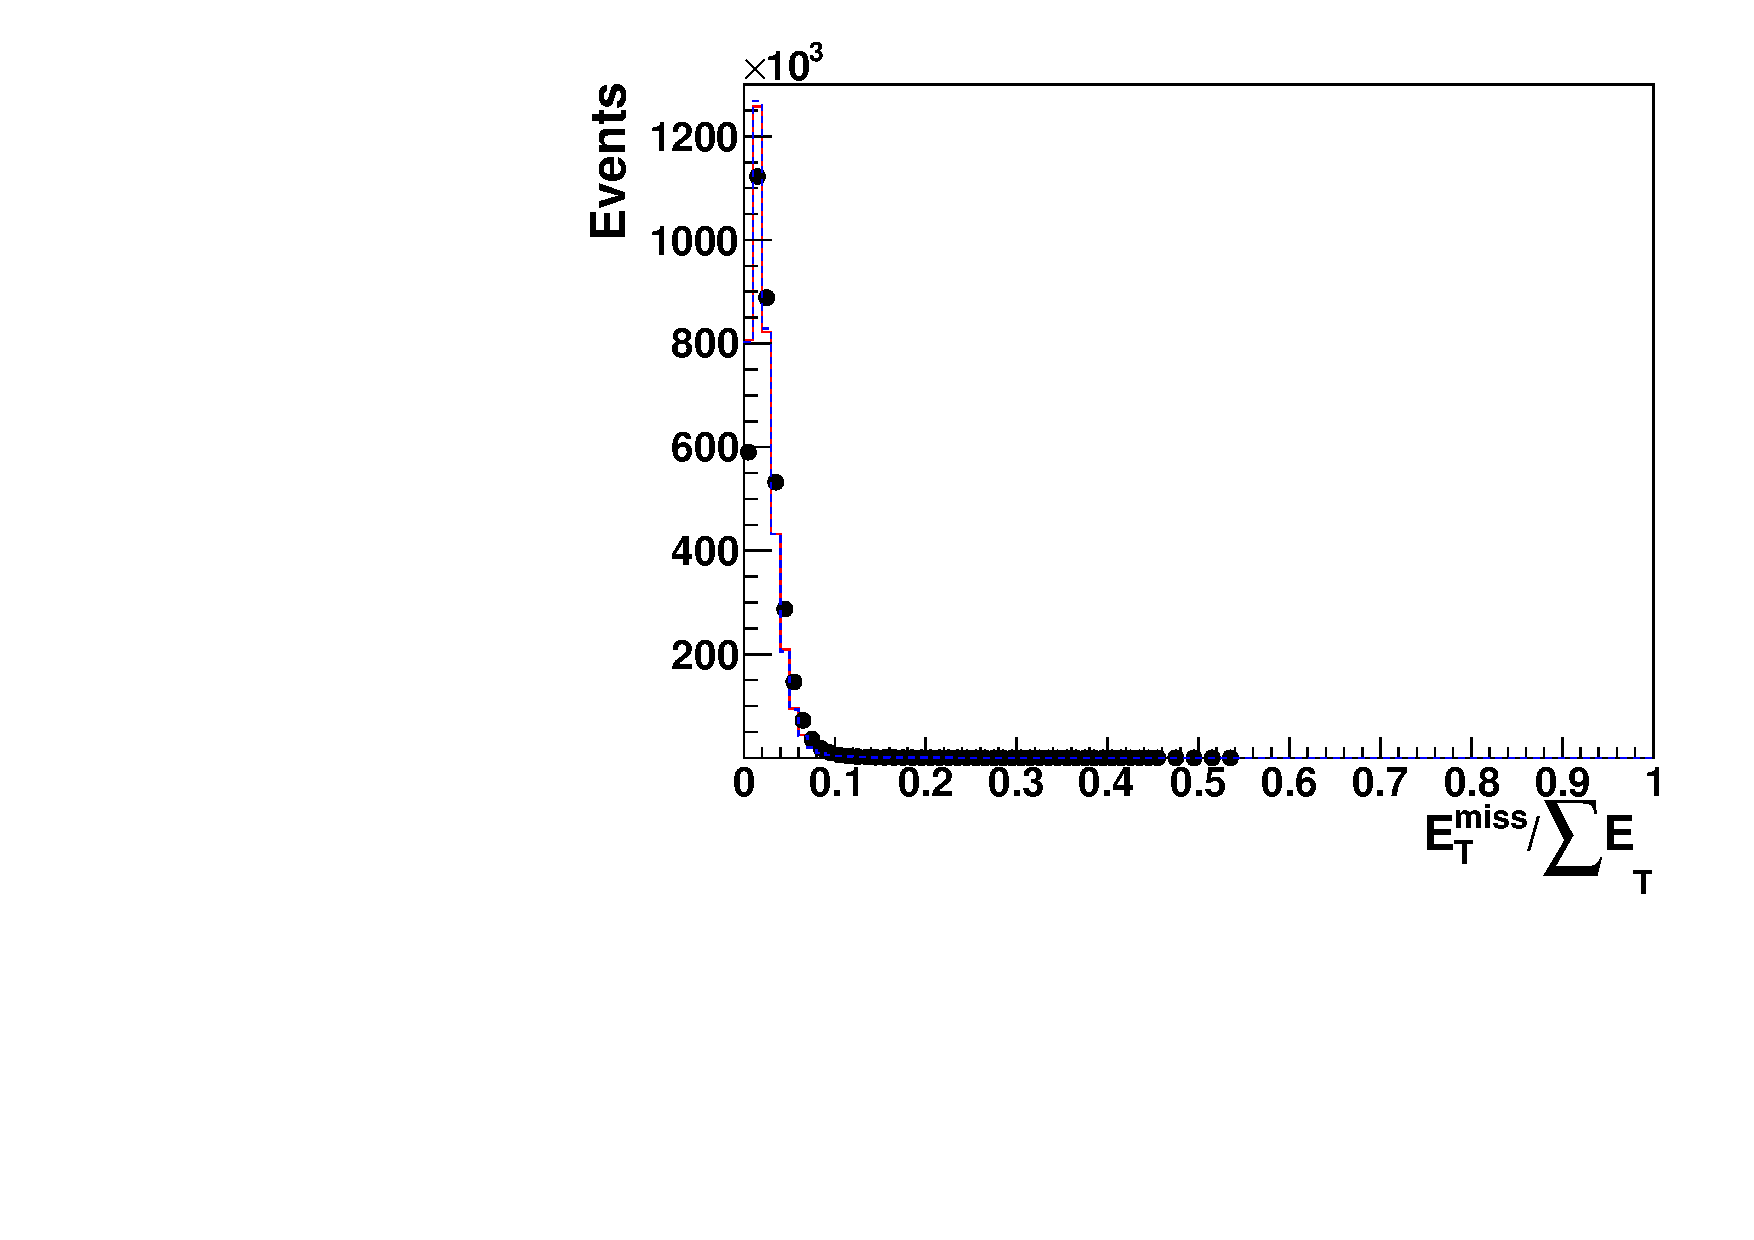
\includegraphics{figs/Data-MC-comparisons/etsumEt.pdf}} &
     \resizebox{0.5\linewidth}{!}{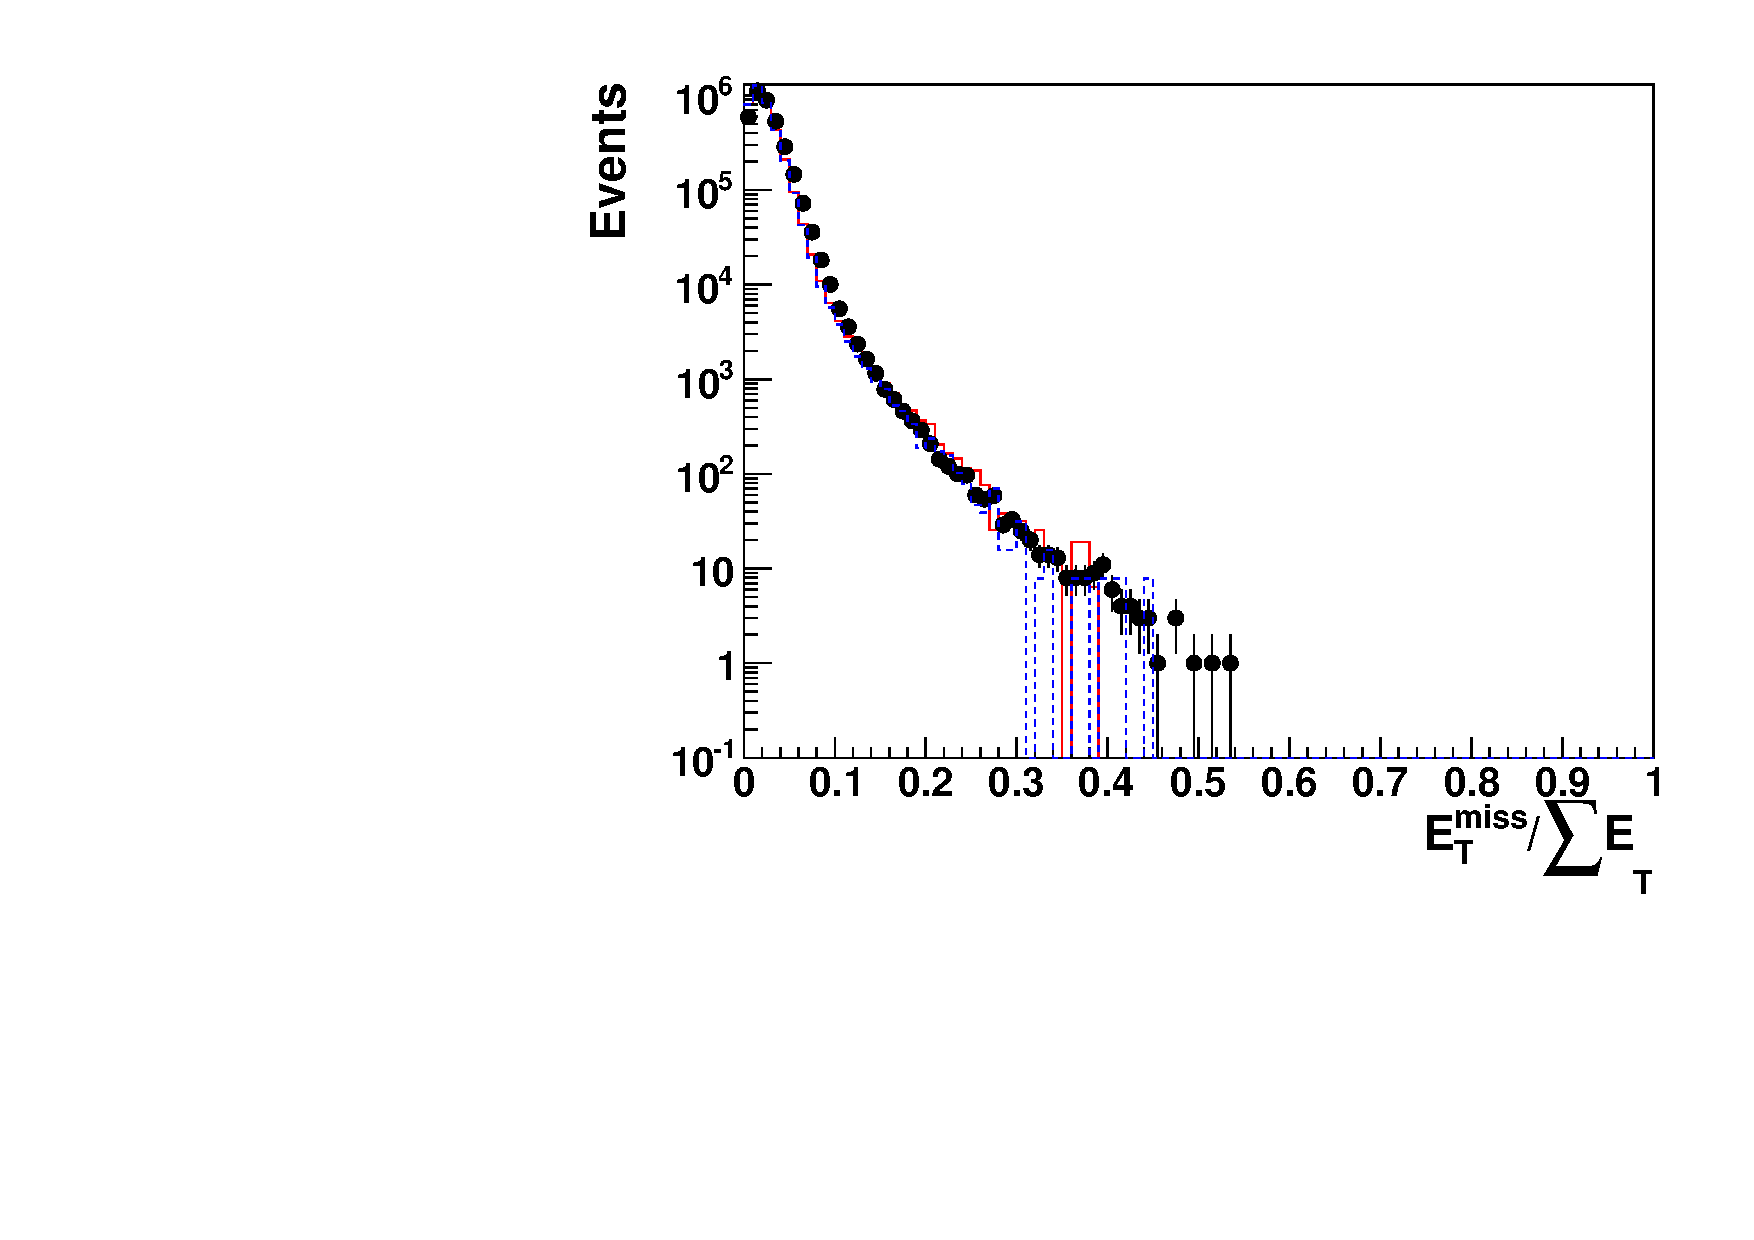
\includegraphics{figs/Data-MC-comparisons/etsumEtlog.pdf}} \\
\end{tabular}
  \caption[Leading two jets mass drop]{Comparisons between data and Monte Carlo for $E_{T}^{miss}/\sum E_{T}$ 
	   The MC is normalized to the number of data events. Plot on the right is the log scale plot. (The plot includes only a subset of the full data sample.)}
  \label{fig:metSumPtSingle}
\end{figure}

%\begin{figure}[htb]
%\centering
%\begin{tabular}{cc}
%     \resizebox{0.5\linewidth}{!}{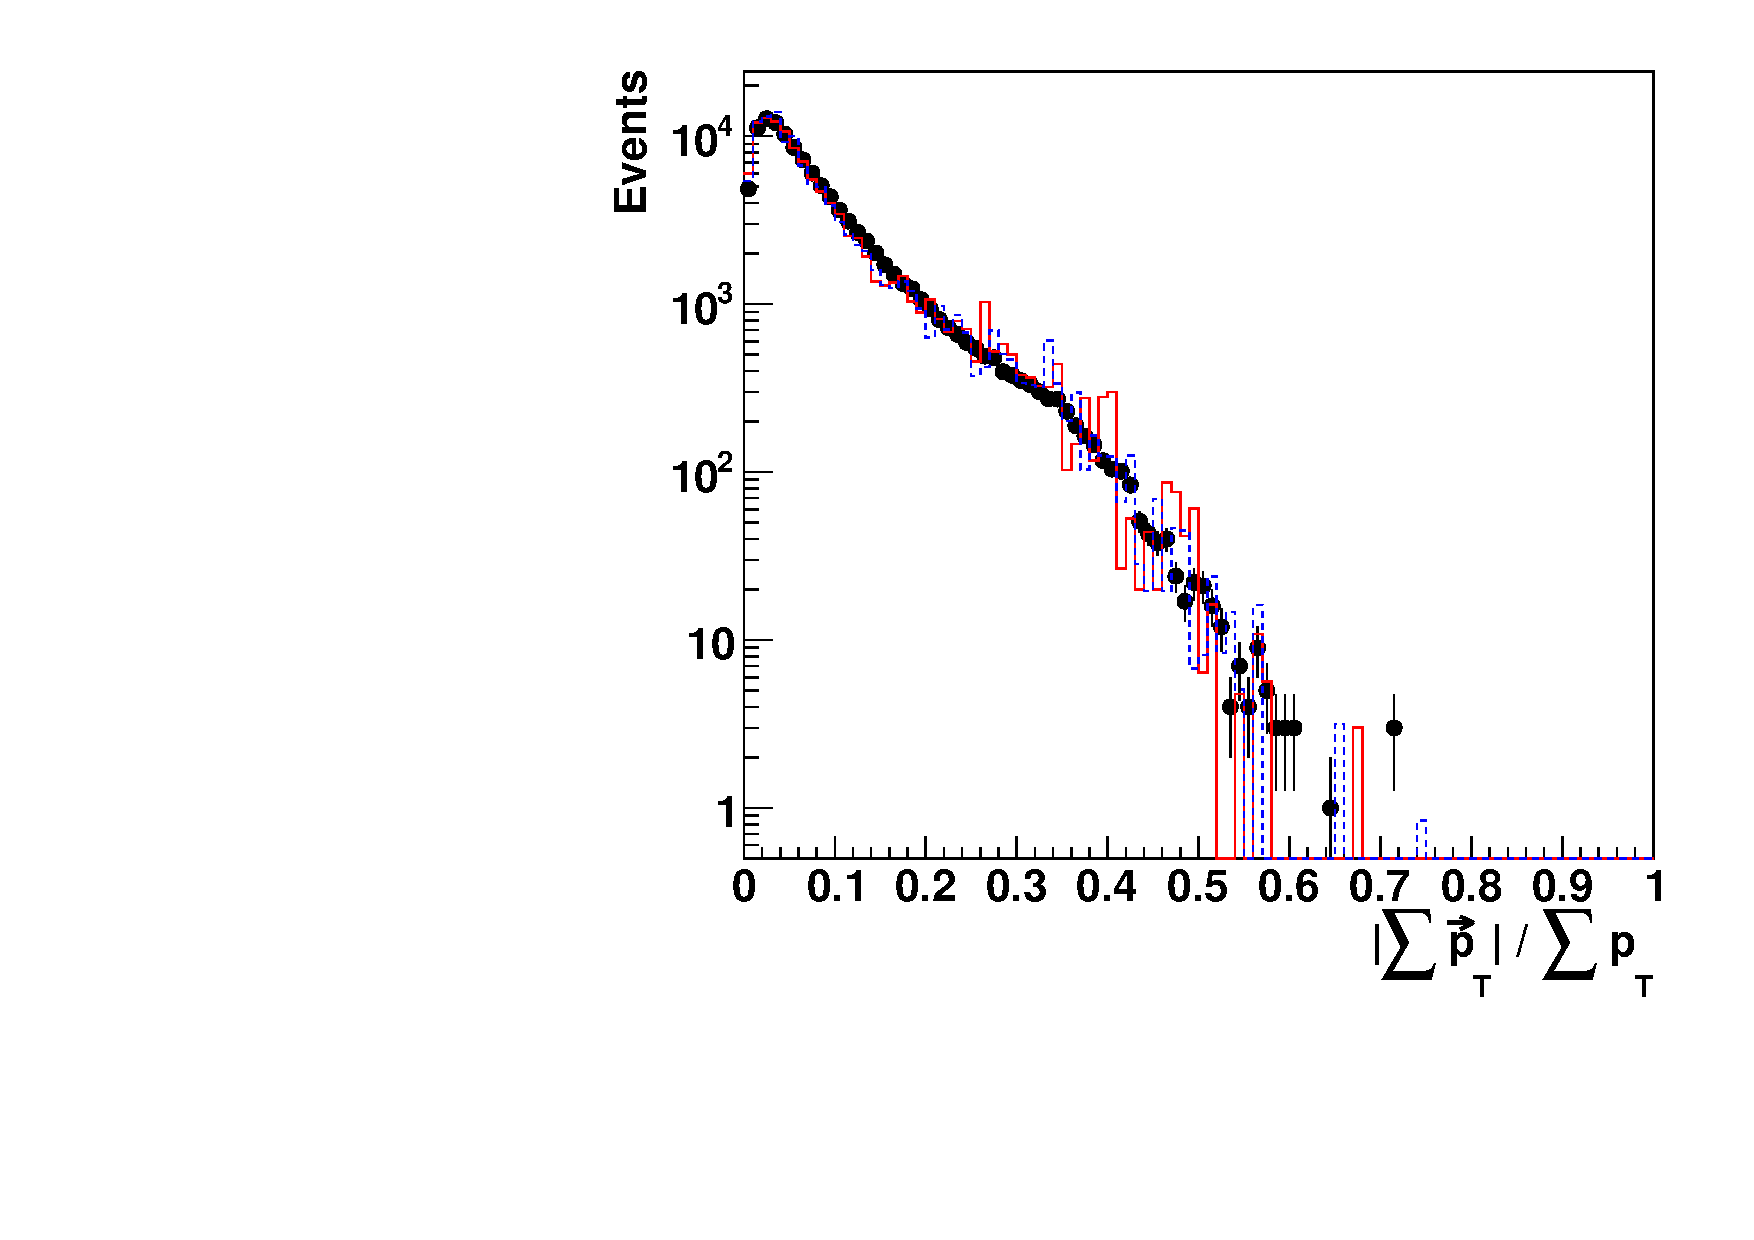
\includegraphics{figs/Data-MC-comparisons/PTVSPT-qVLowP.pdf}} &
%     \resizebox{0.5\linewidth}{!}{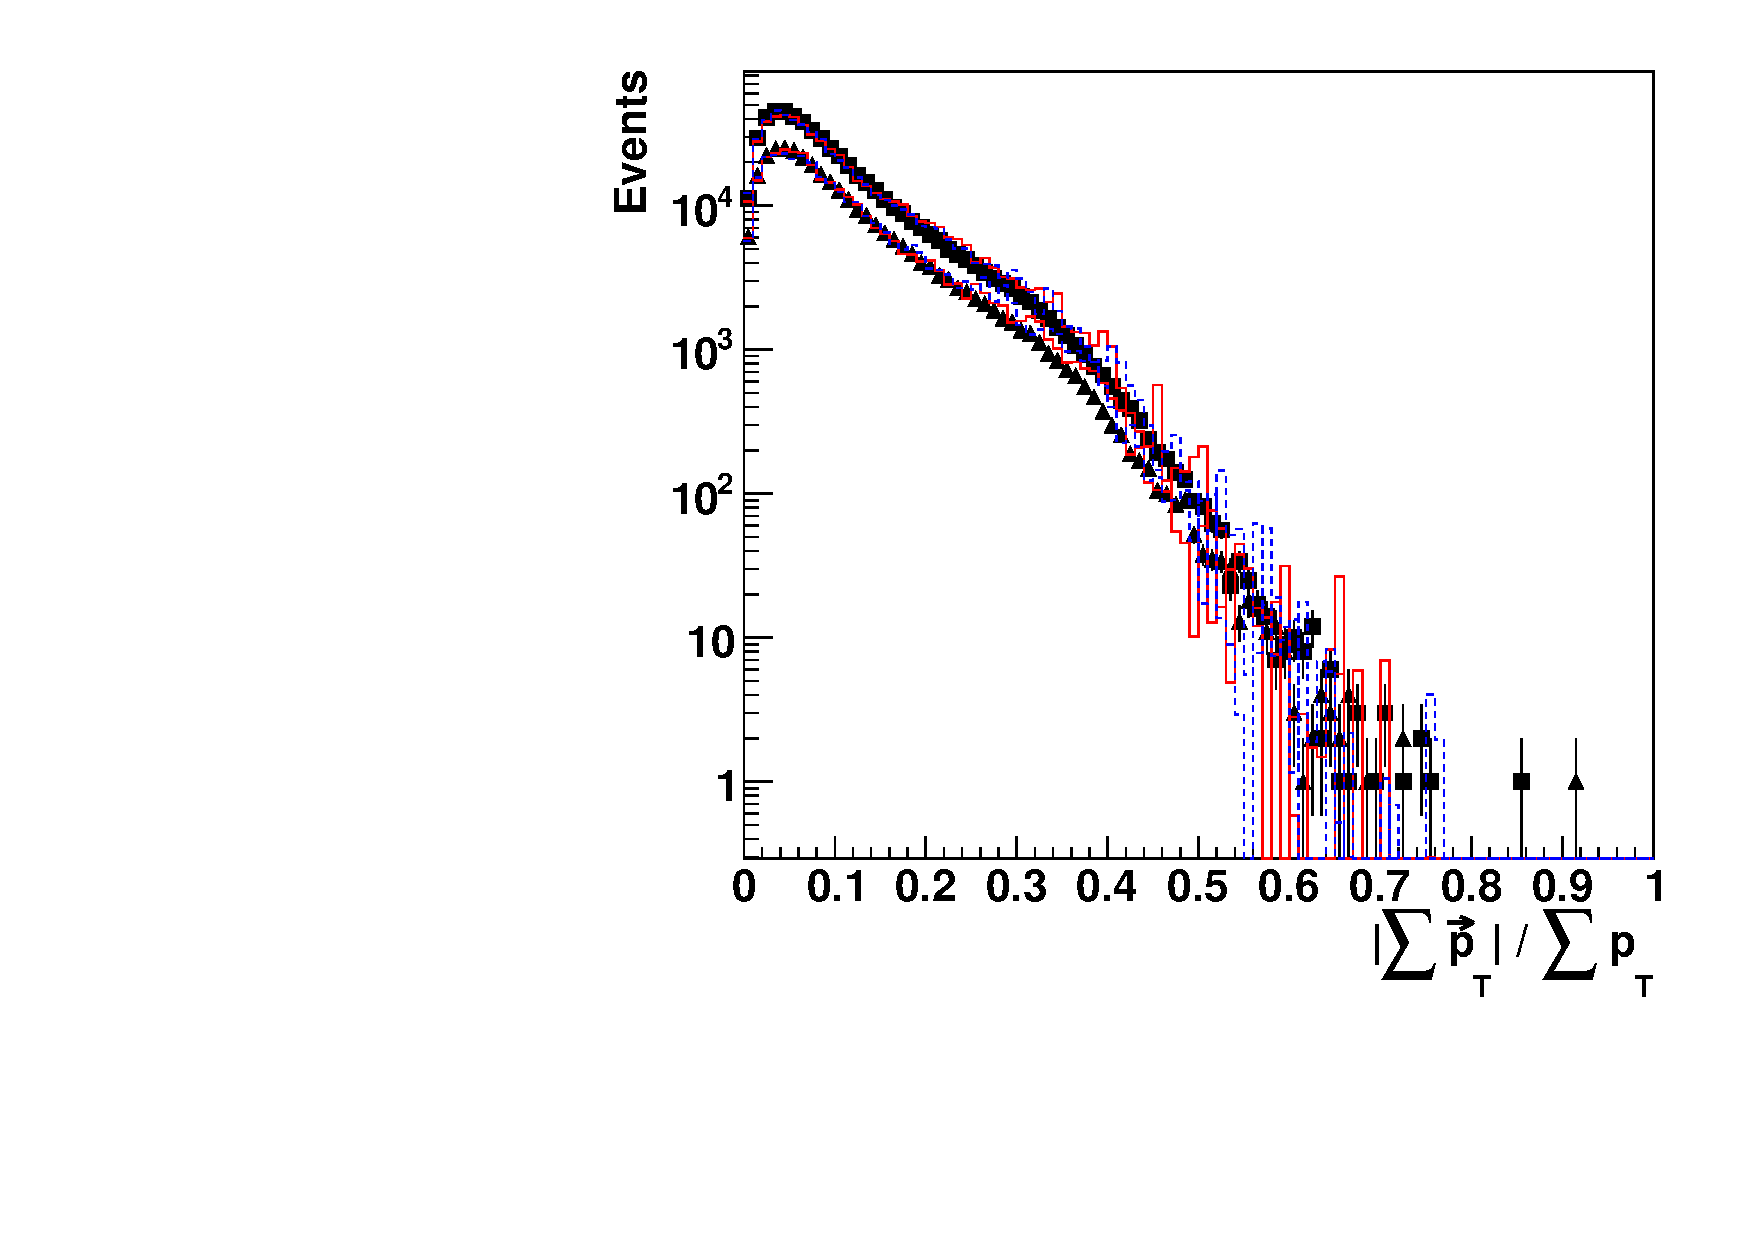
\includegraphics{figs/Data-MC-comparisons/PTVSPT-qVMiumHigh.pdf}} \\
%\end{tabular}
%  \caption[Delta Eta Single]{Comparisons between data and Monte Carlo
%                    for $|\sum{\vec{p}_{T}}| / \sum{p_{T}}$ of the two leading jets of low purity (left) and low-high purity (right) 1-tagged events.
%	   The MC is normalized to the number of data events in each category. }
%  \label{fig:metSumPtSingle}
%\end{figure}

%\begin{figure}[htb]
%\centering
%\begin{tabular}{cc}
%     \resizebox{0.5\linewidth}{!}{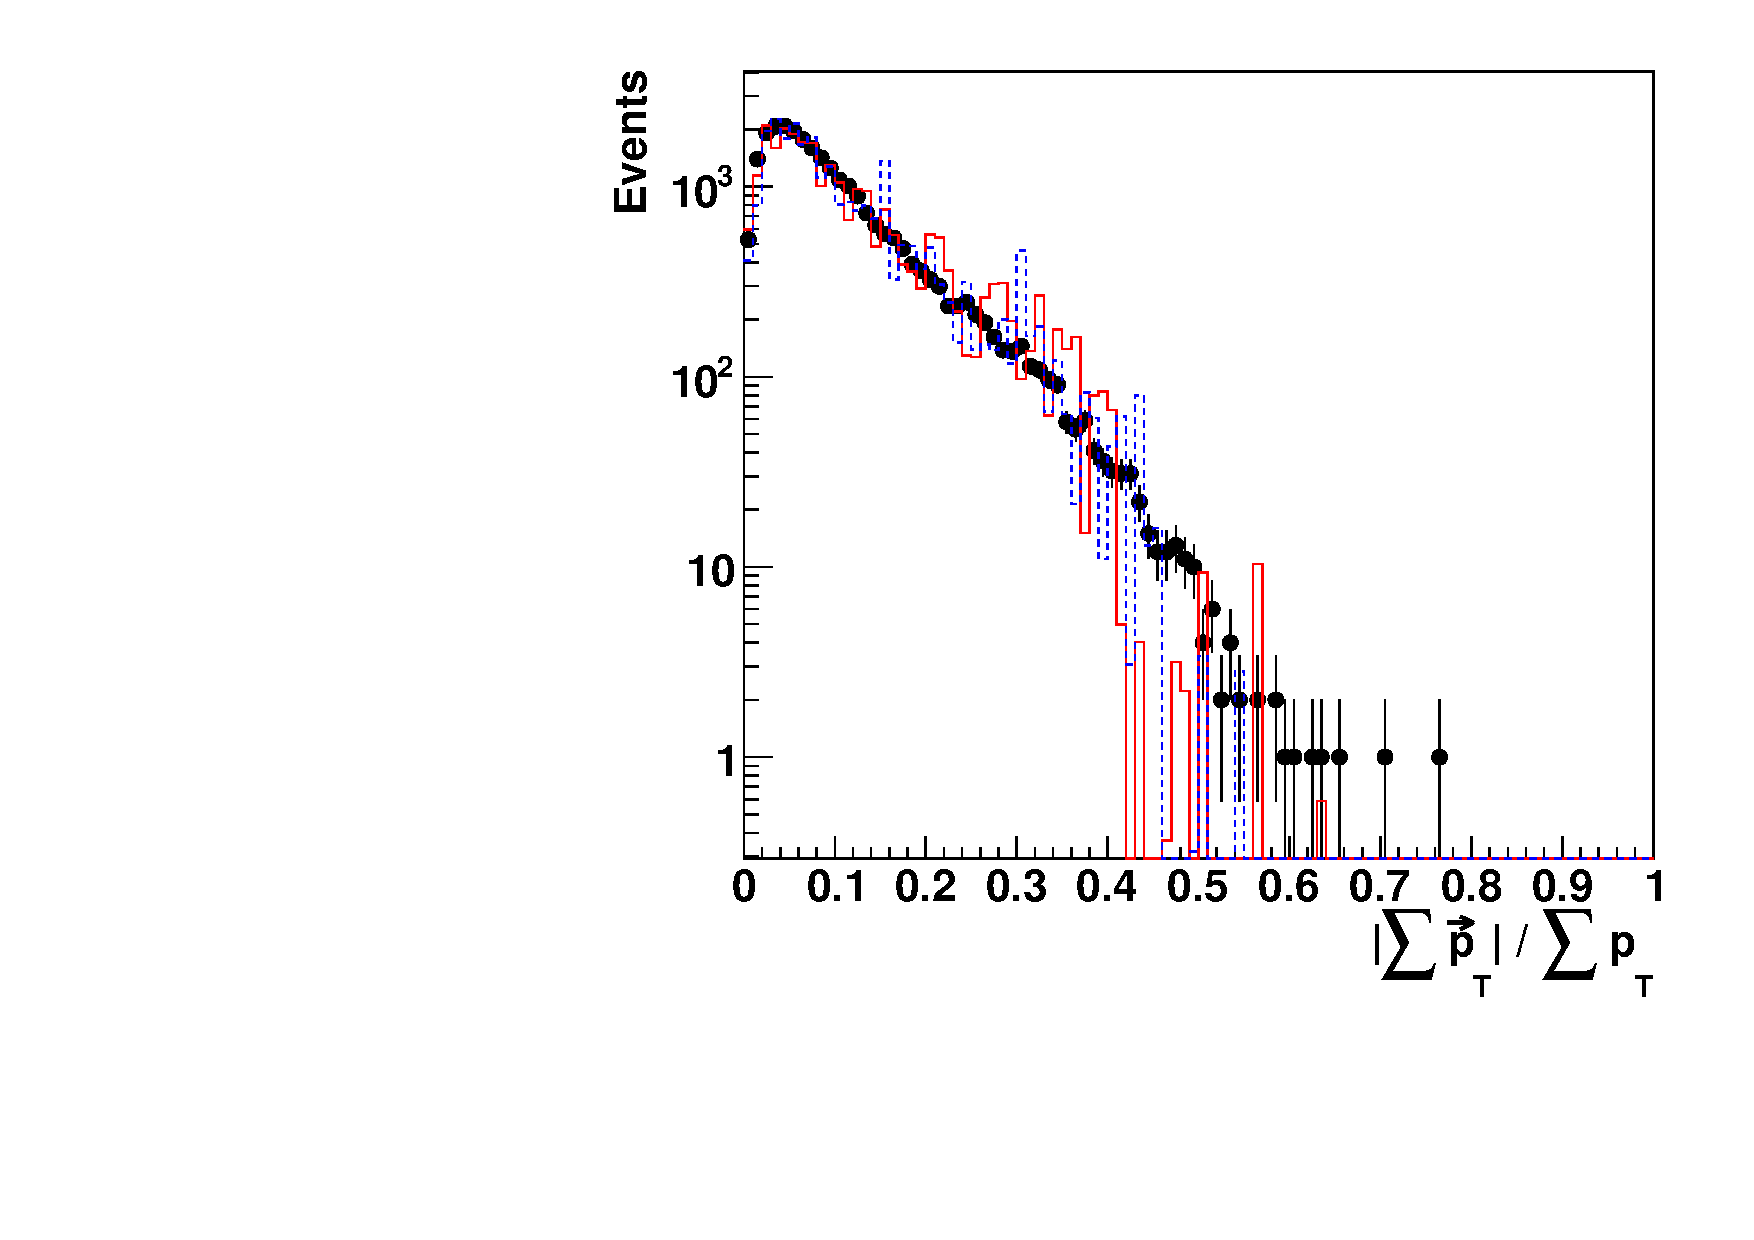
\includegraphics{figs/Data-MC-comparisons/PTVSPT-VVLowP.pdf}} &
%     \resizebox{0.5\linewidth}{!}{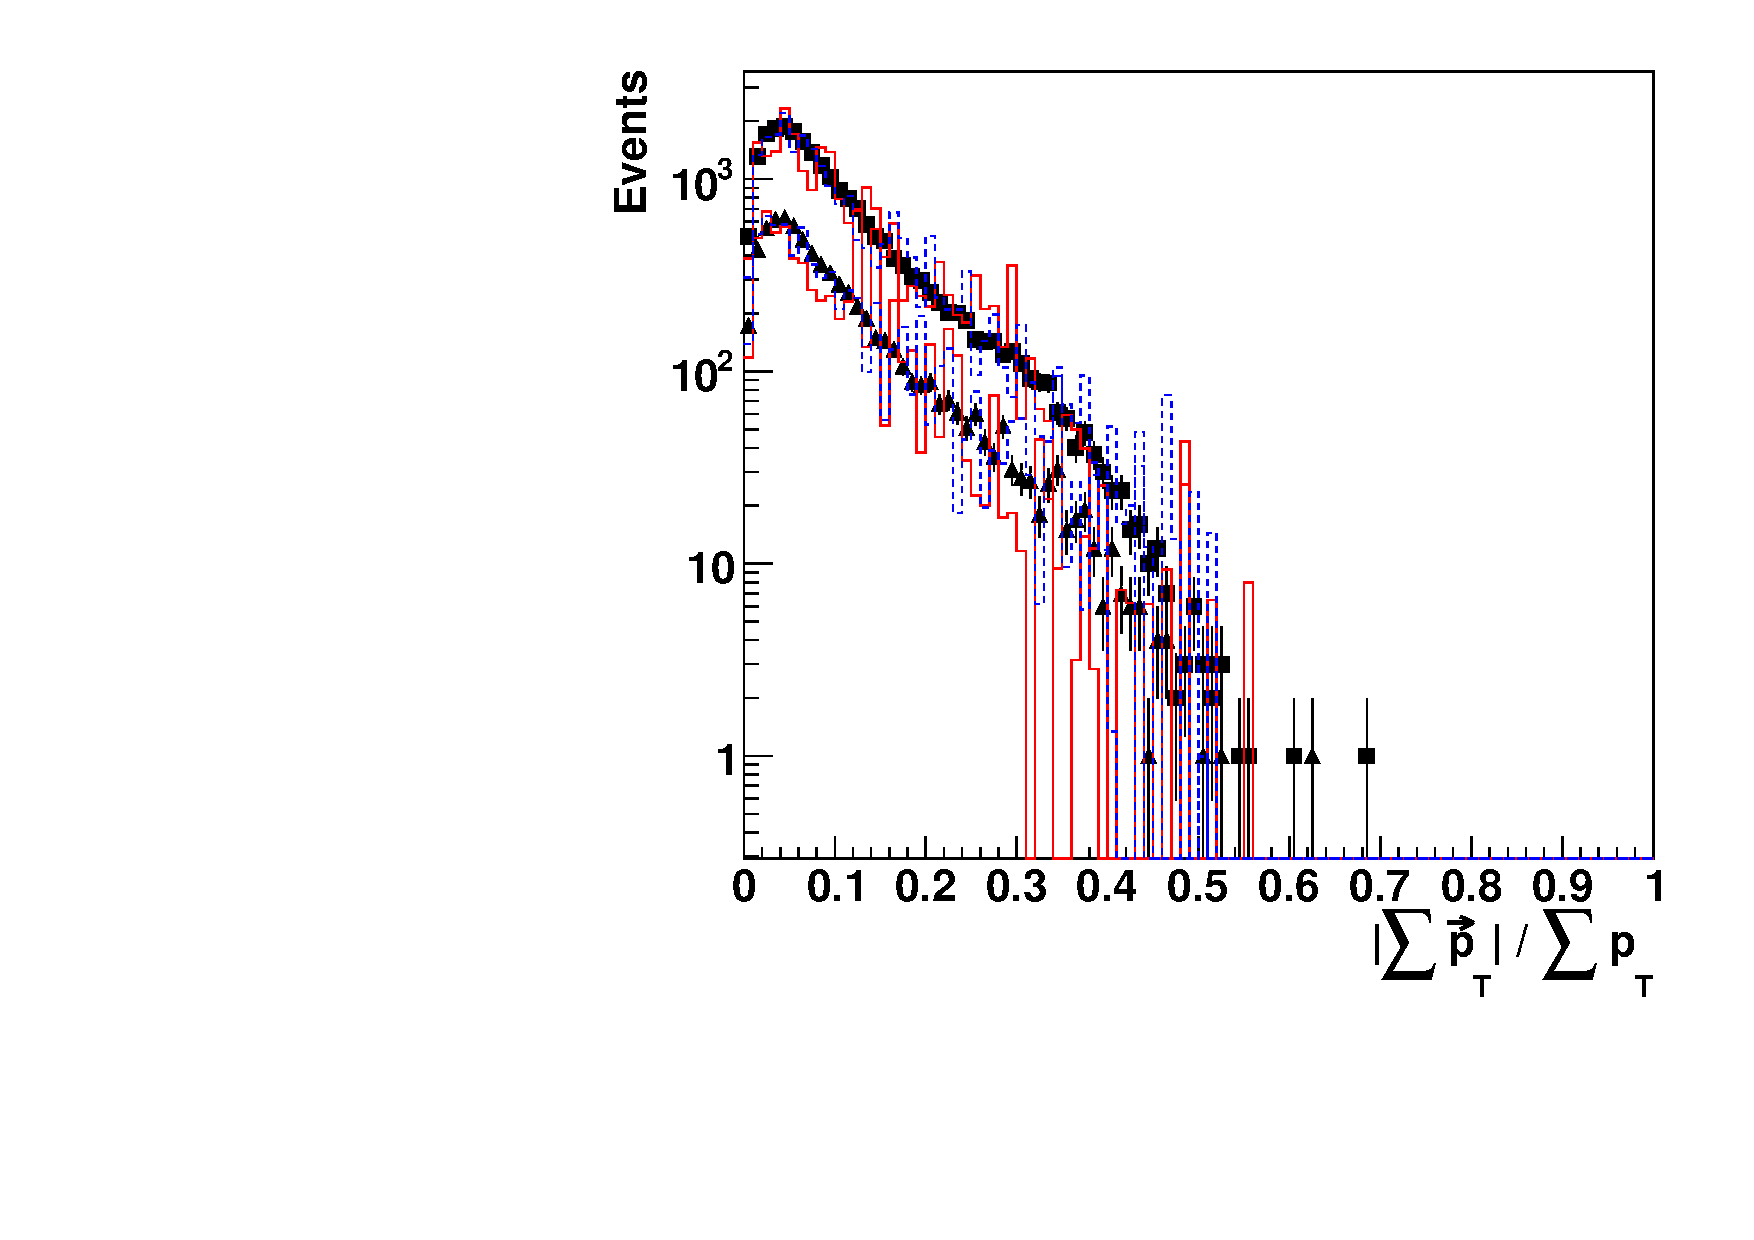
\includegraphics{figs/Data-MC-comparisons/PTVSPT-VVMiumHigh.pdf}} \\
%\end{tabular}
%  \caption[Delta Eta Double]{Comparisons between data and Monte Carlo
%                     for $|\sum{\vec{p}_{T}}| / \sum{p_{T}}$ of the two leading jets of low purity (left) and low-high purity (right) 2-tagged events. The MC is normalized to the number of data events in each category. }
%  \label{fig:metSumPtDouble}
%\end{figure}

\newpage
\begin{figure}[htb]
\centering
\begin{tabular}{cc}
     \resizebox{0.5\linewidth}{!}{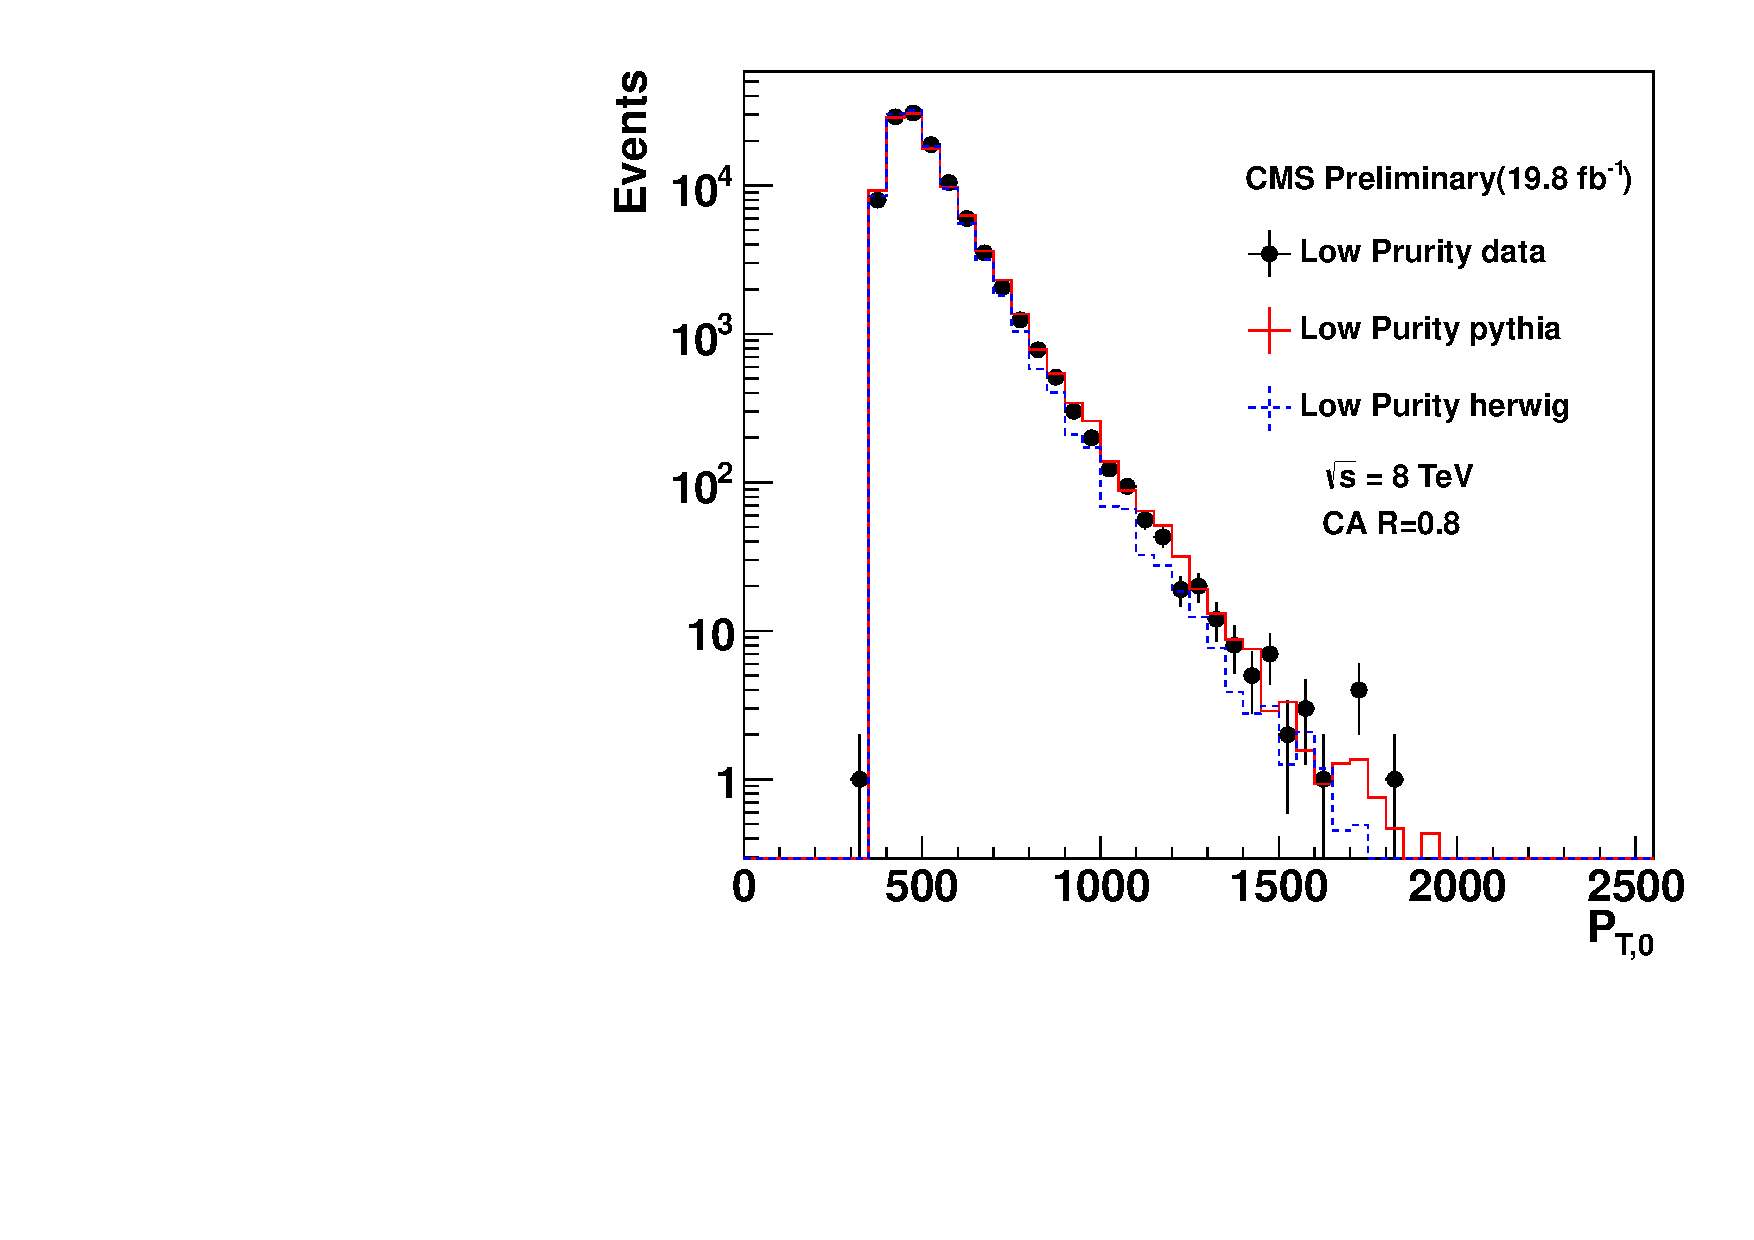
\includegraphics{figs/Data-MC-comparisons/PT0-qVLowP.pdf}} &
     \resizebox{0.5\linewidth}{!}{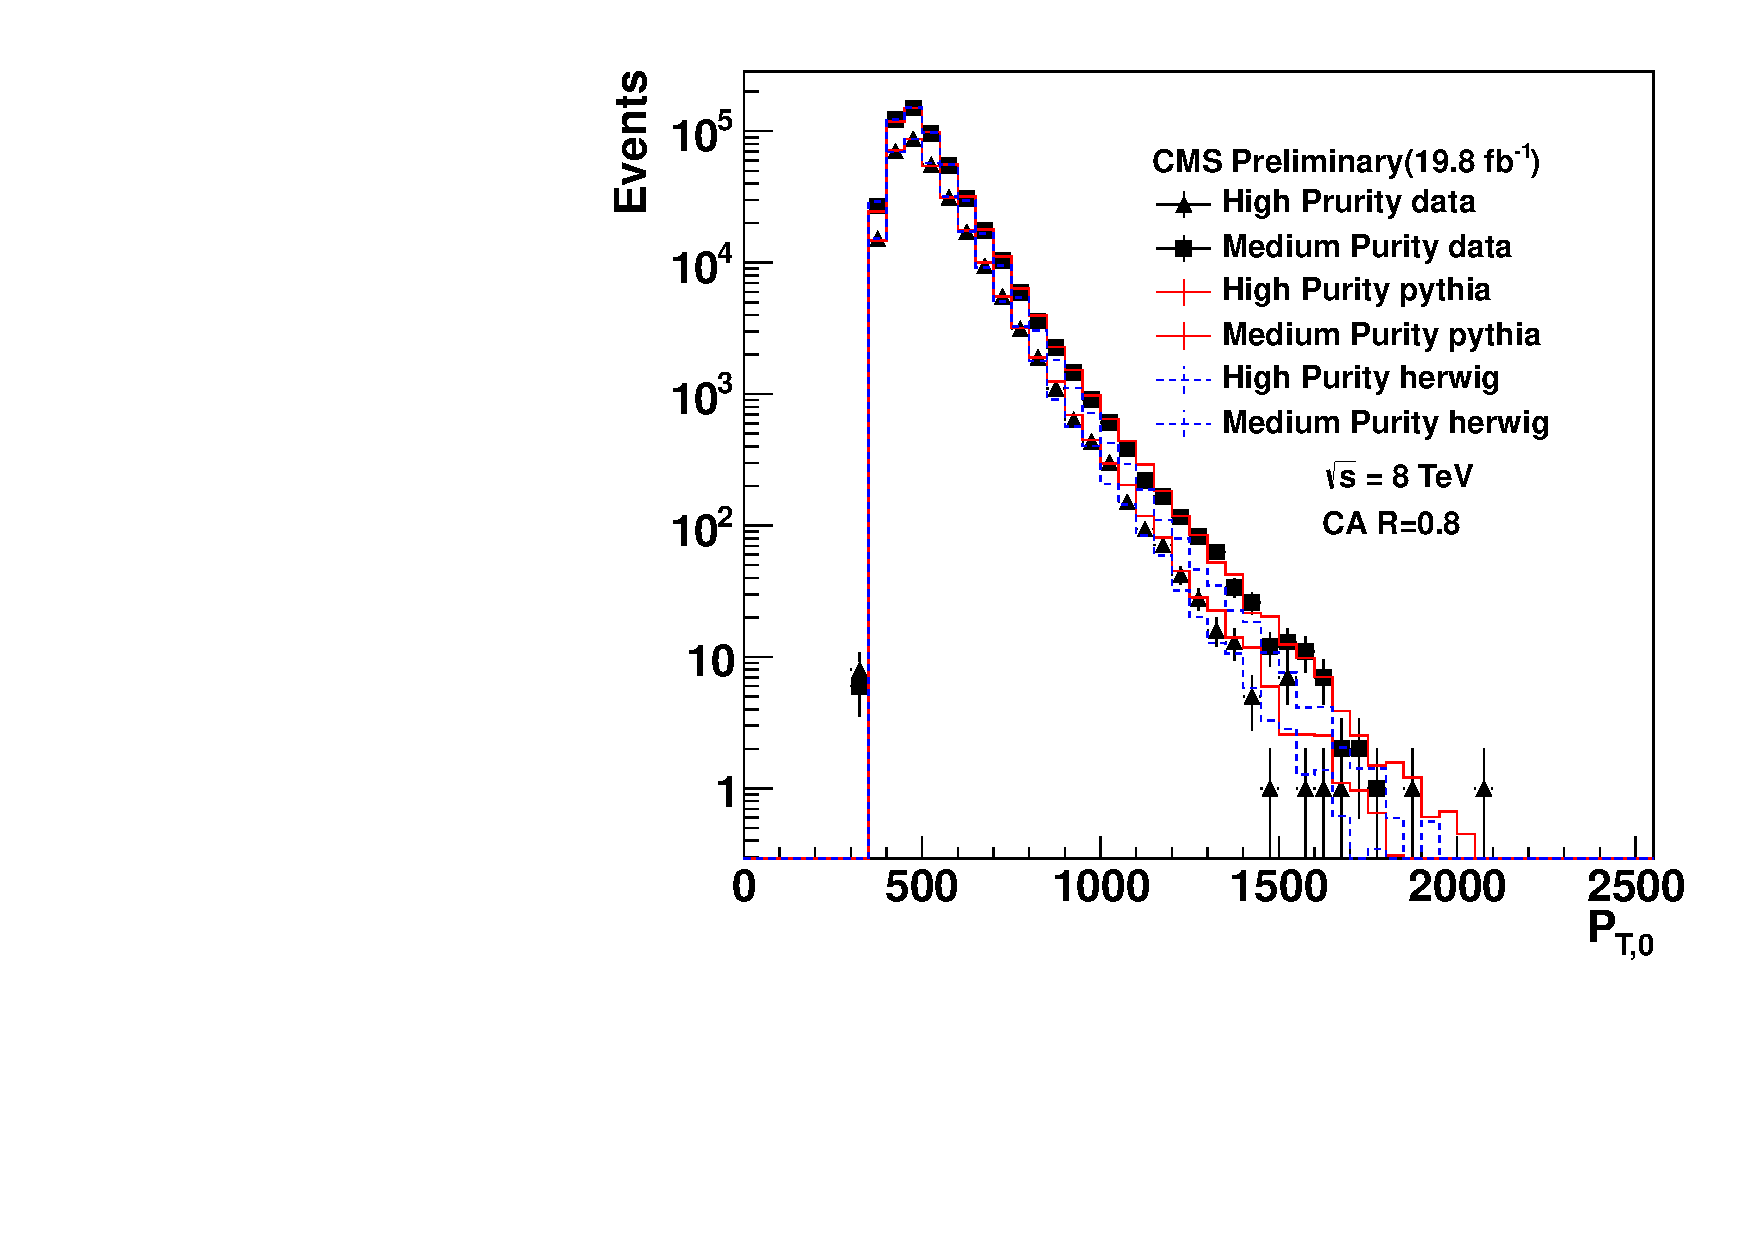
\includegraphics{figs/Data-MC-comparisons/PT0-qVMiumHigh.pdf}} \\
\end{tabular}
  \caption[PT Single]{Comparisons between data and Monte Carlo
                    for $\pt$ of the leading jet of low purity (left) and low-high purity (right) 1-tagged events.
	   The MC is normalized to the number of data events in each category. }
  \label{fig:Pt0Single}
\end{figure}

\begin{figure}[htb]
\centering
\begin{tabular}{cc}
     \resizebox{0.5\linewidth}{!}{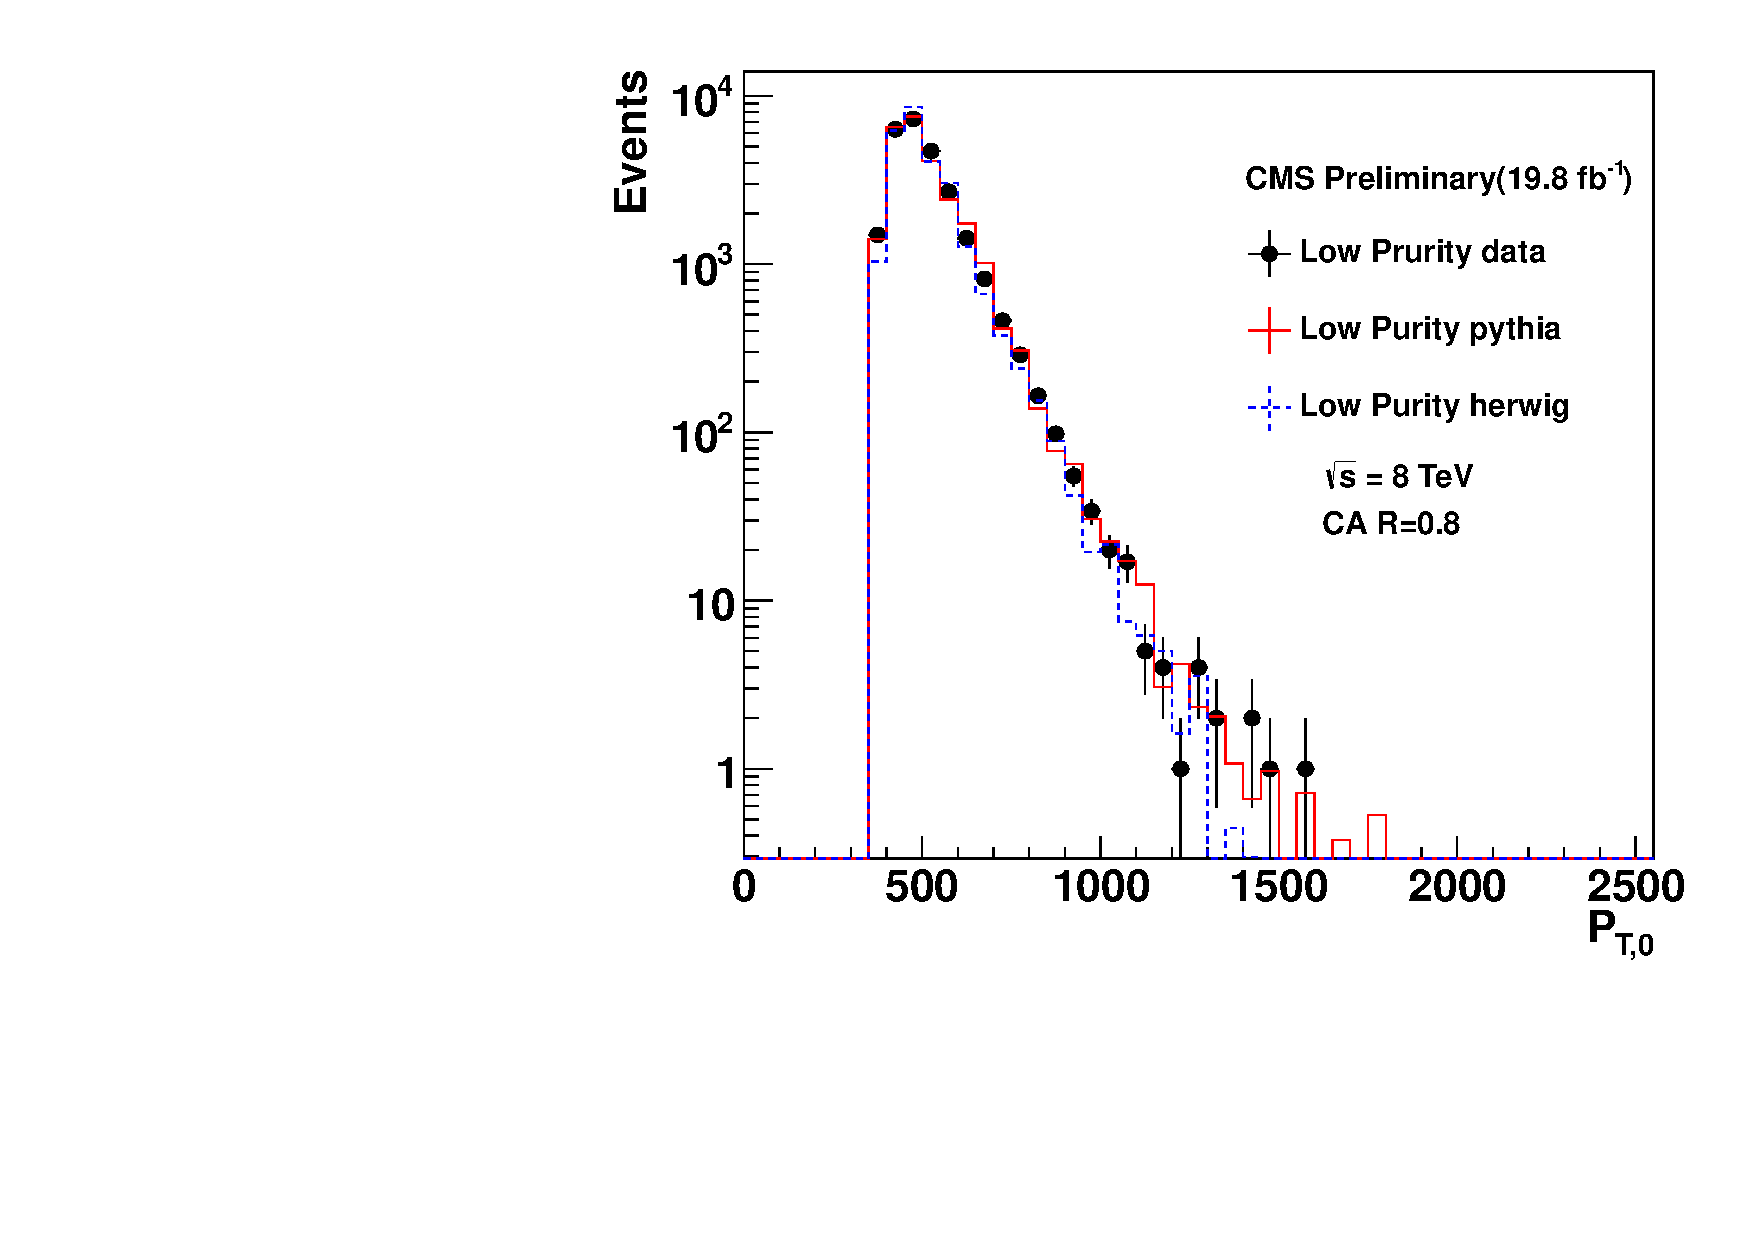
\includegraphics{figs/Data-MC-comparisons/PT0-VVLowP.pdf}} &
     \resizebox{0.5\linewidth}{!}{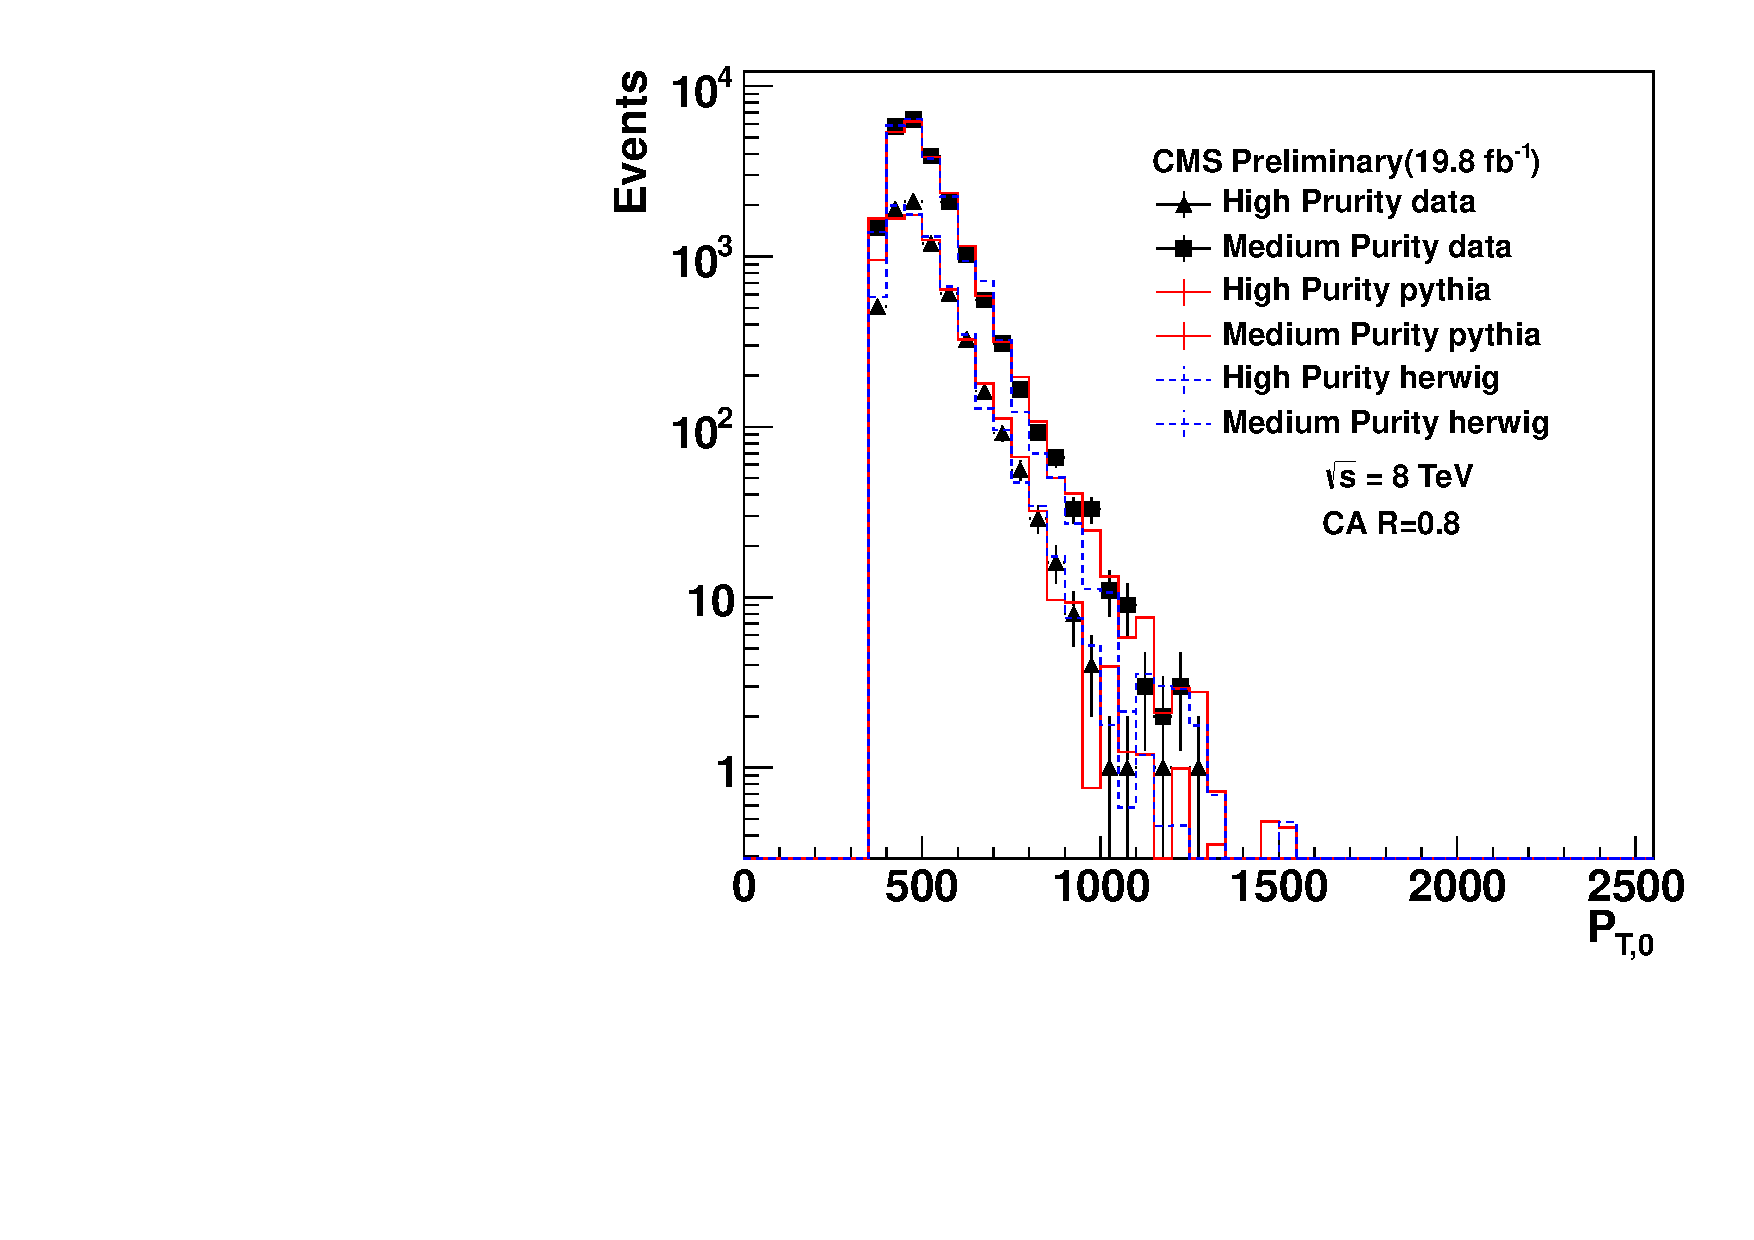
\includegraphics{figs/Data-MC-comparisons/PT0-VVMiumHigh.pdf}} \\
\end{tabular}
  \caption[Delta Eta Double]{Comparisons between data and Monte Carlo
                     for $\pt$ of the leading jet of low purity (left) and low-high purity (right) 2-tagged events. The MC is normalized to the number of data events in each category. }
  \label{fig:Pt0Double}
\end{figure}

\newpage
\begin{figure}[htb]
\centering
\begin{tabular}{cc}
     \resizebox{0.5\linewidth}{!}{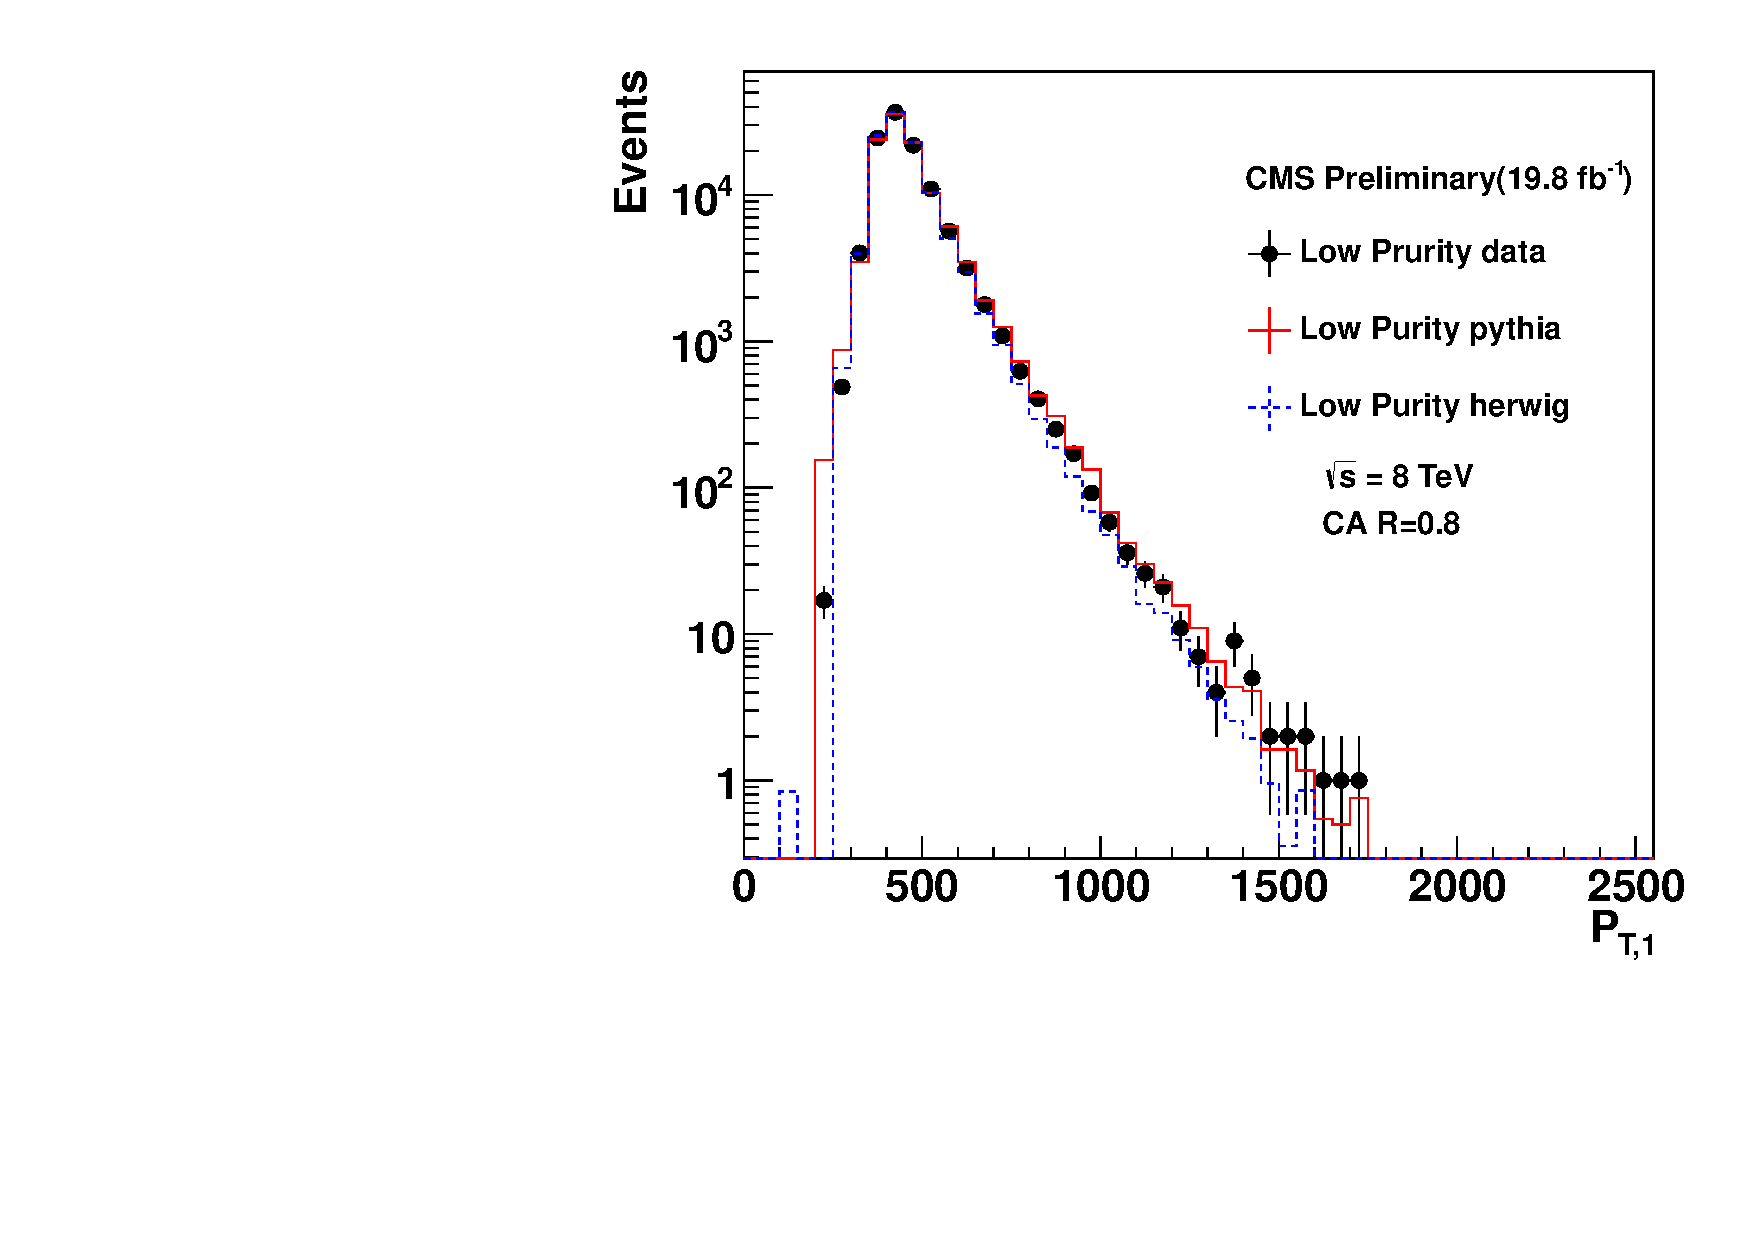
\includegraphics{figs/Data-MC-comparisons/PT1-qVLowP.pdf}} &
     \resizebox{0.5\linewidth}{!}{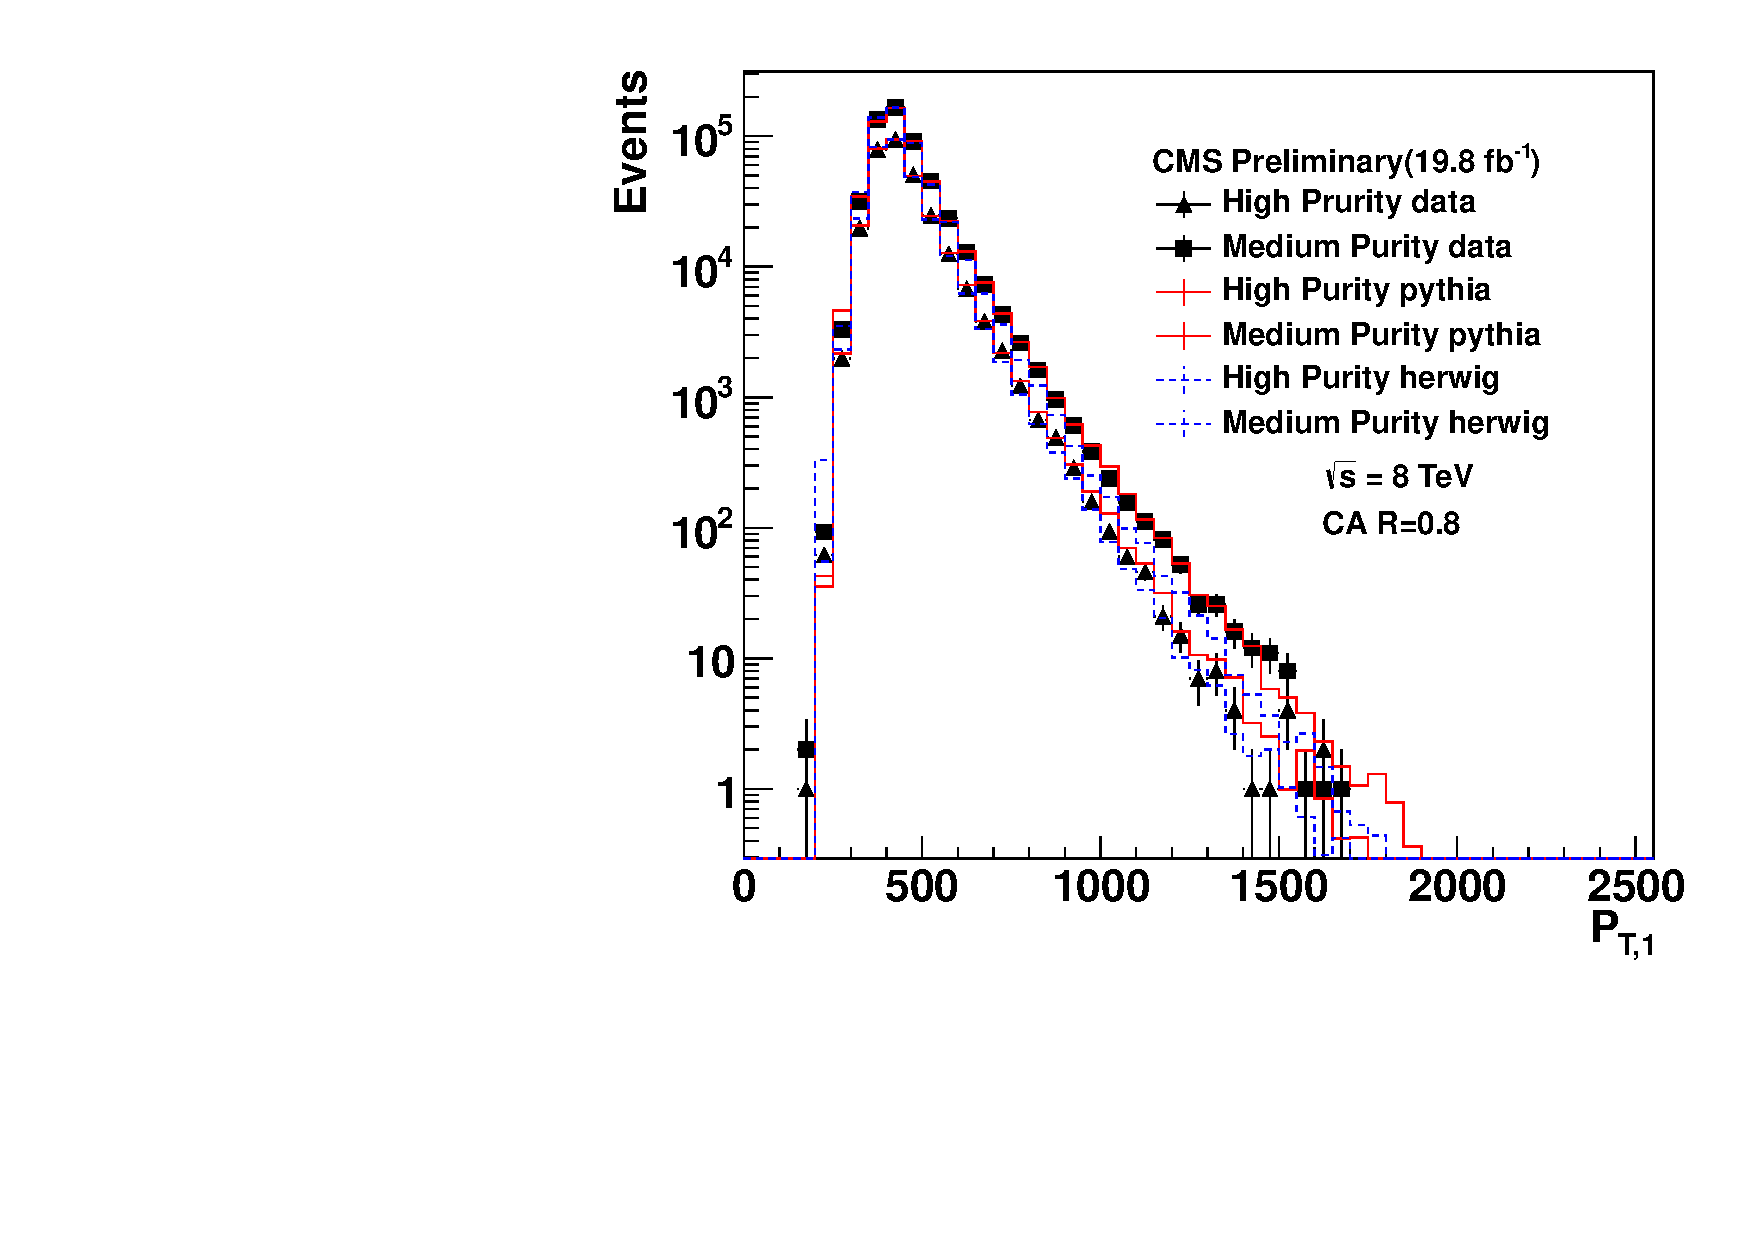
\includegraphics{figs/Data-MC-comparisons/PT1-qVMiumHigh.pdf}} \\
\end{tabular}
  \caption[PT Single]{Comparisons between data and Monte Carlo
                    for $\pt$ of the second leading jet of low purity (left) and low-high purity (right) 1-tagged events.
	   The MC is normalized to the number of data events in each category. }
  \label{fig:Pt1Single}
\end{figure}

\begin{figure}[htb]
\centering
\begin{tabular}{cc}
     \resizebox{0.5\linewidth}{!}{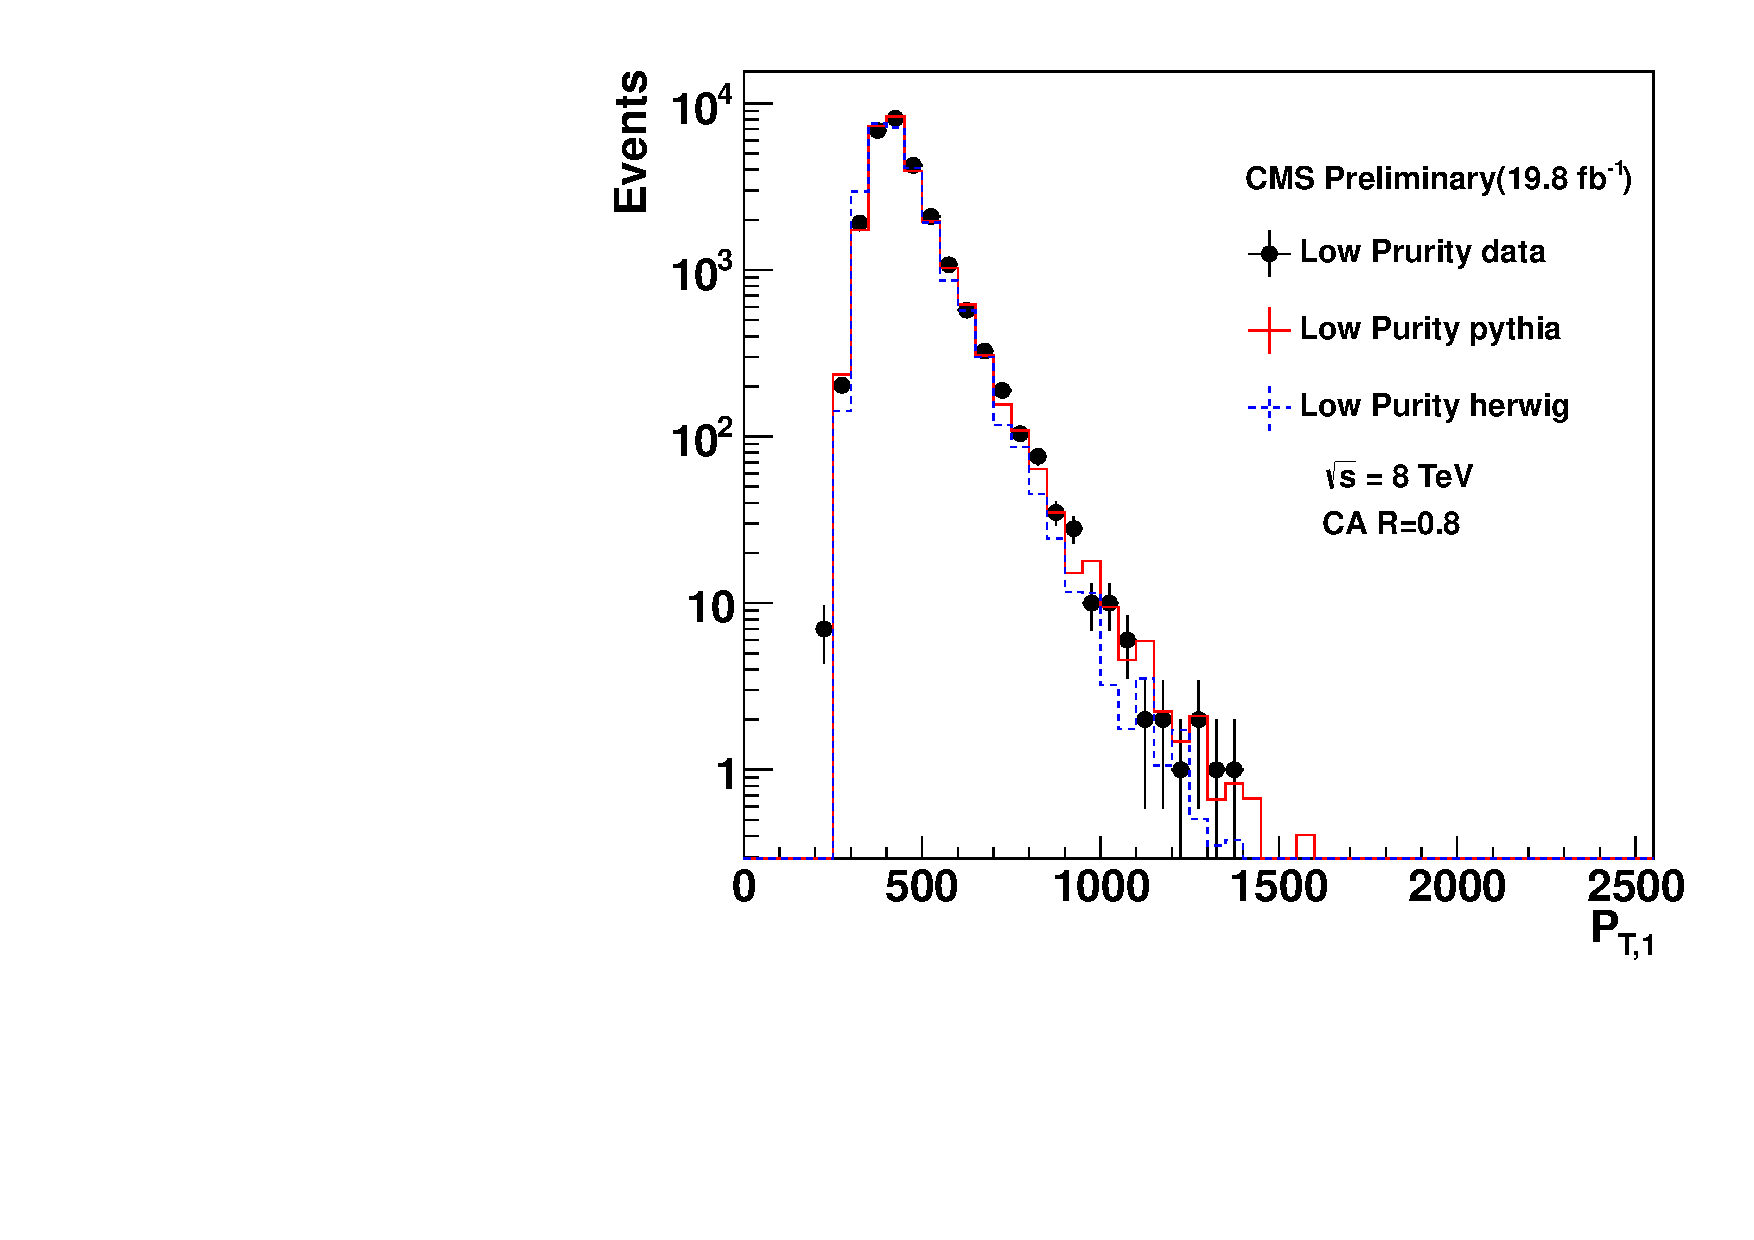
\includegraphics{figs/Data-MC-comparisons/PT1-VVLowP.pdf}} &
     \resizebox{0.5\linewidth}{!}{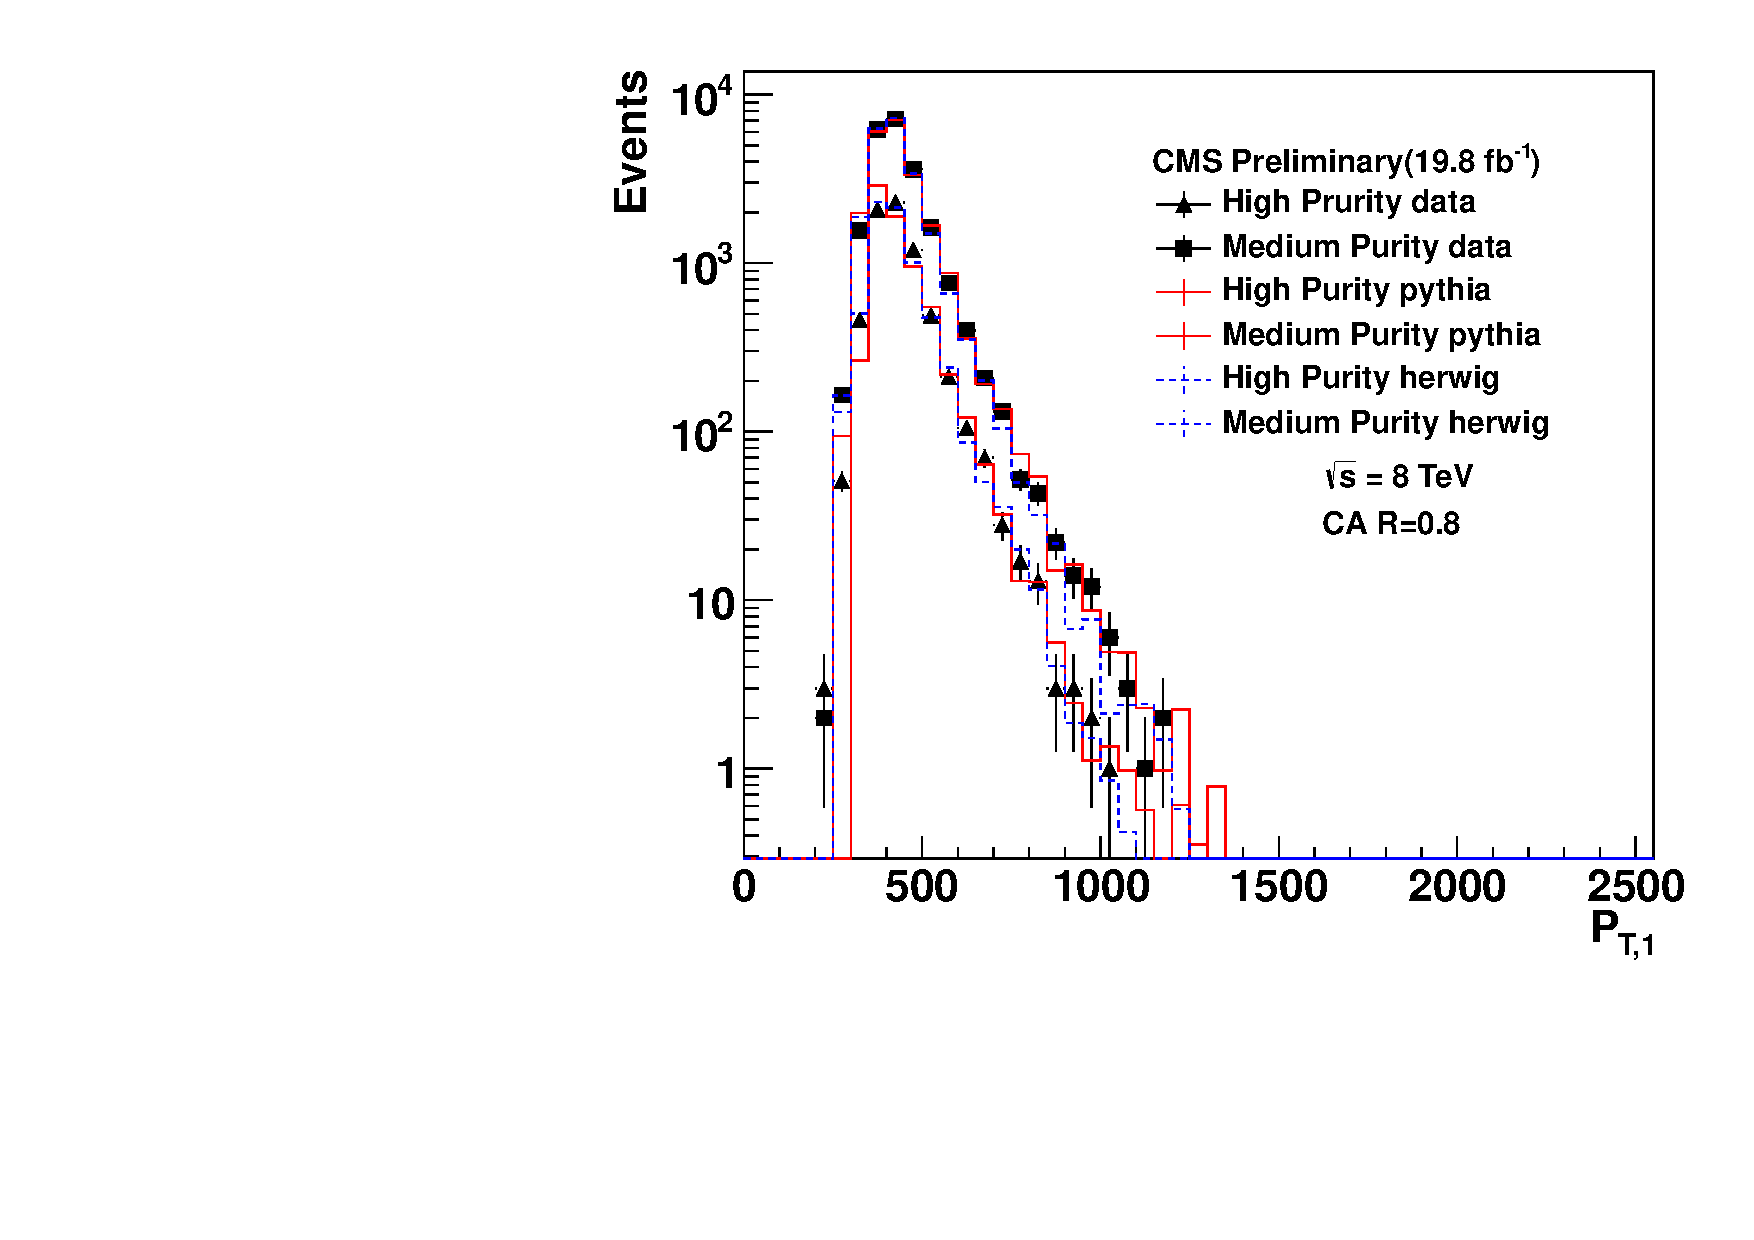
\includegraphics{figs/Data-MC-comparisons/PT1-VVMiumHigh.pdf}} \\
\end{tabular}
  \caption[Delta Eta Double]{Comparisons between data and Monte Carlo
                     for $\pt$ of the second leading jet of low purity (left) and low-high purity (right) 2-tagged events. The MC is normalized to the number of data events in each category. }
  \label{fig:Pt1Double}
\end{figure}



\newpage
\begin{figure}[htb]
\centering
\begin{tabular}{cc}
     \resizebox{0.5\linewidth}{!}{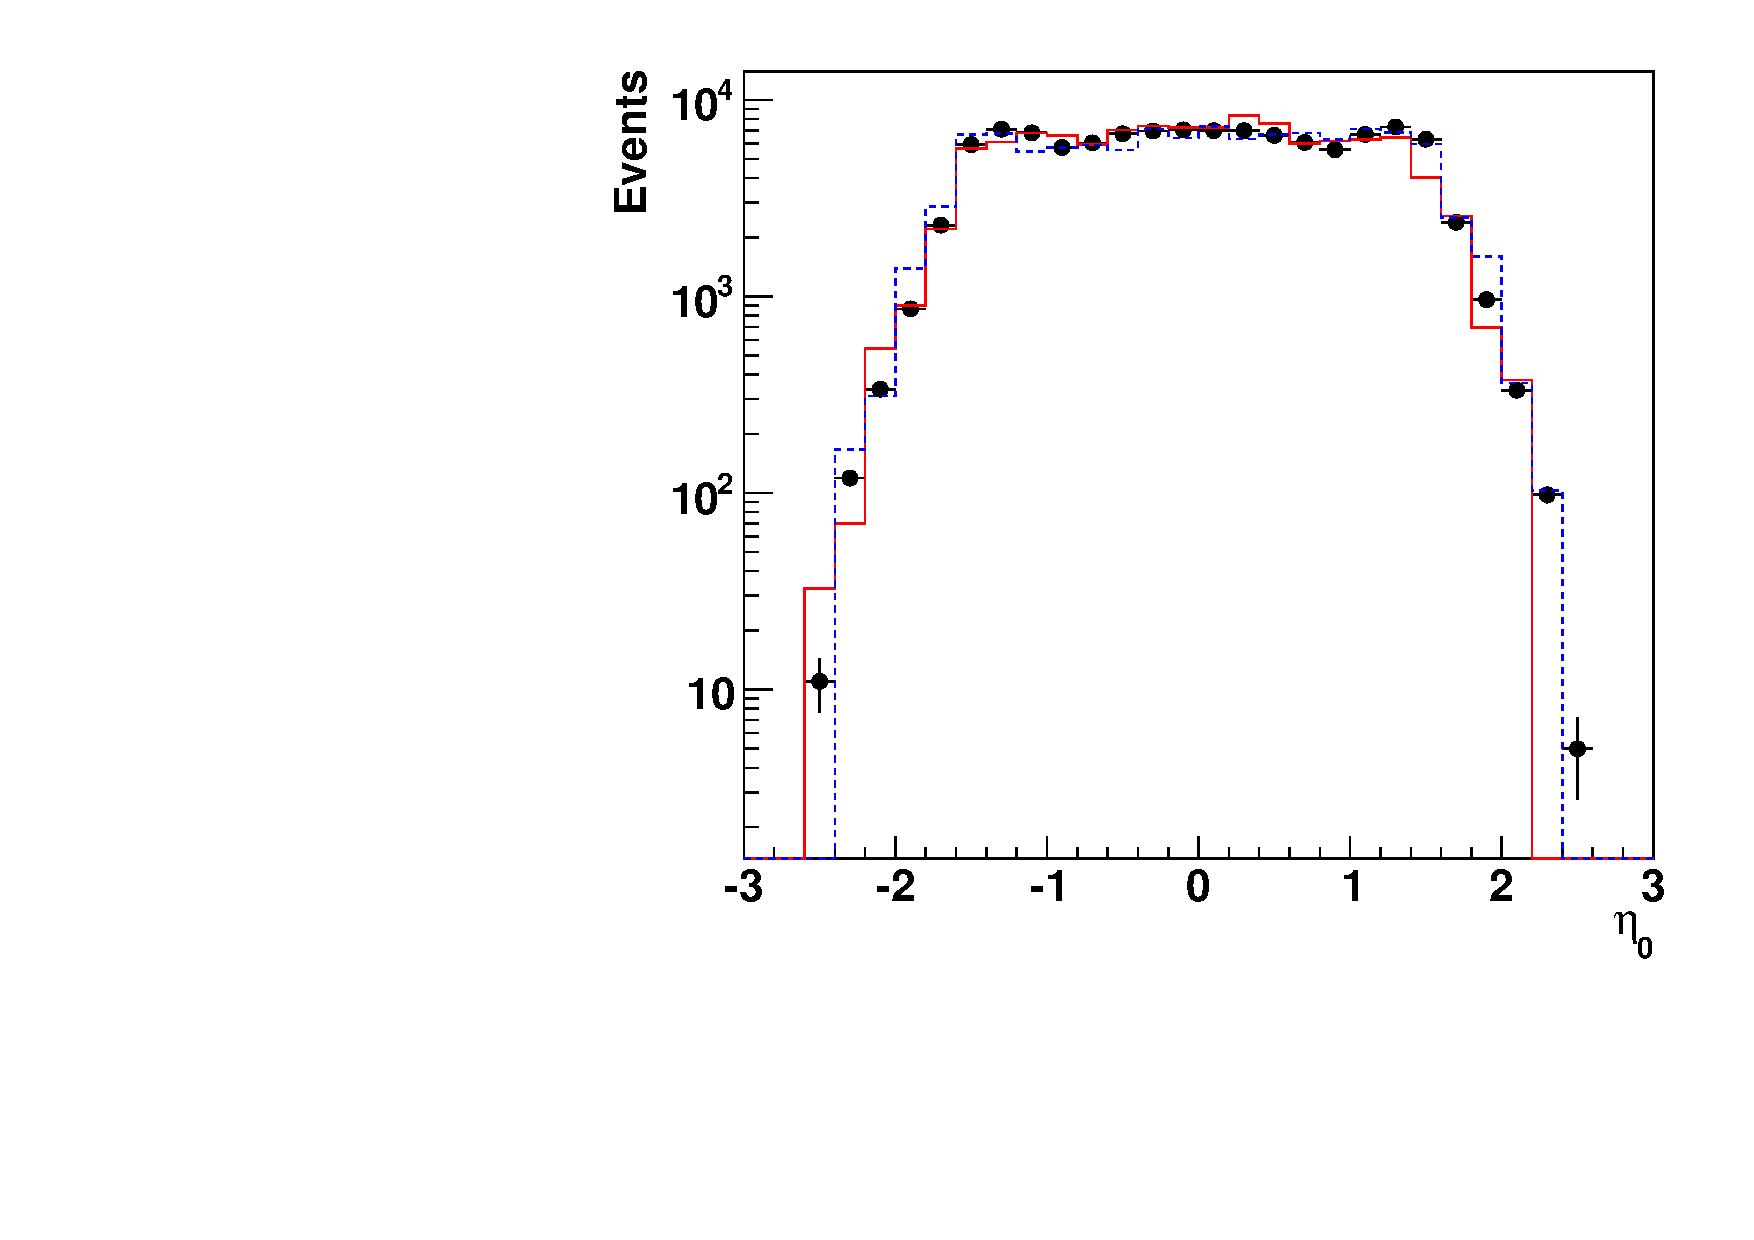
\includegraphics{figs/Data-MC-comparisons/Eta0-qVLowP.pdf}} &
     \resizebox{0.5\linewidth}{!}{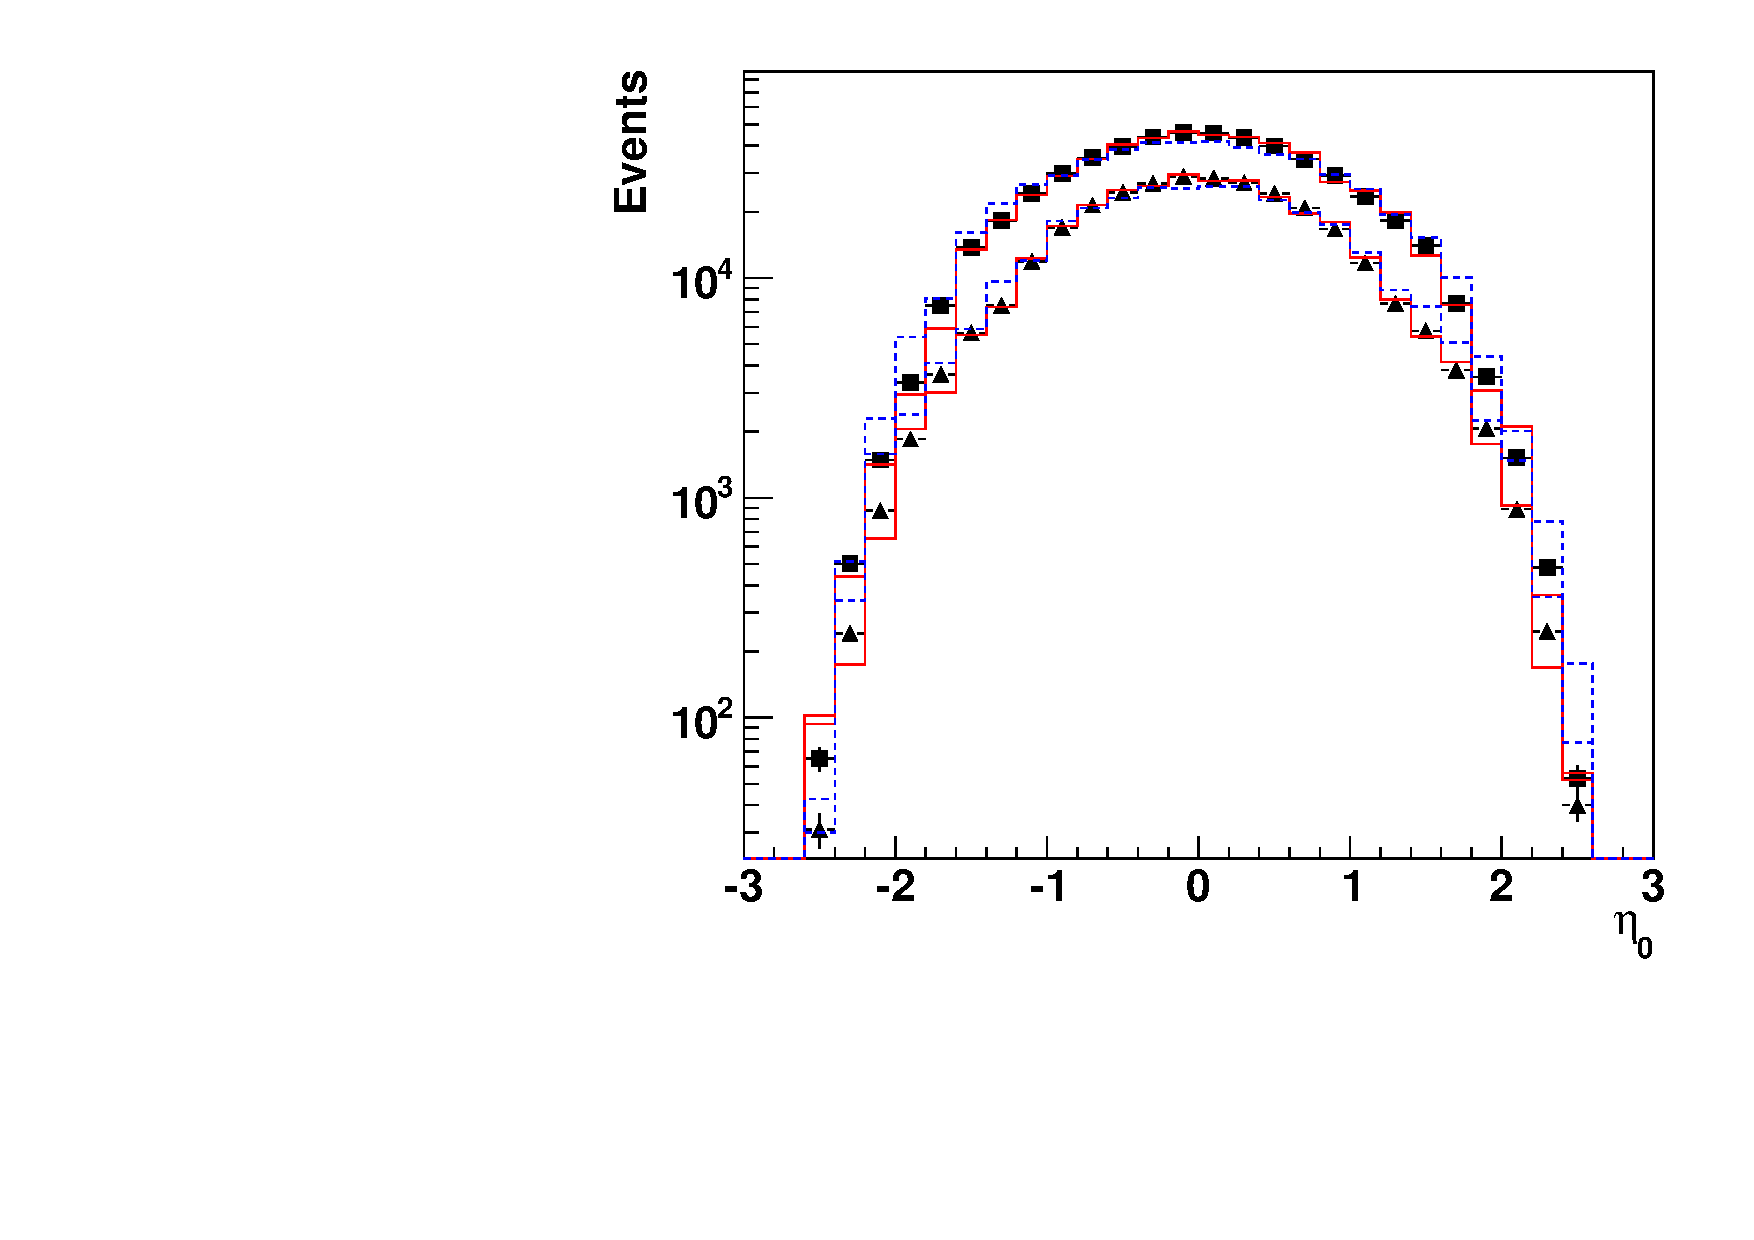
\includegraphics{figs/Data-MC-comparisons/Eta0-qVMiumHigh.pdf}} \\
\end{tabular}
  \caption[PT Single]{Comparisons between data and Monte Carlo
                    for $\eta$ of the leading jet of low purity (left) and low-high purity (right) 1-tagged events.
	   The MC is normalized to the number of data events in each category. }
  \label{fig:Eta0Single}
\end{figure}

\begin{figure}[htb]
\centering
\begin{tabular}{cc}
     \resizebox{0.5\linewidth}{!}{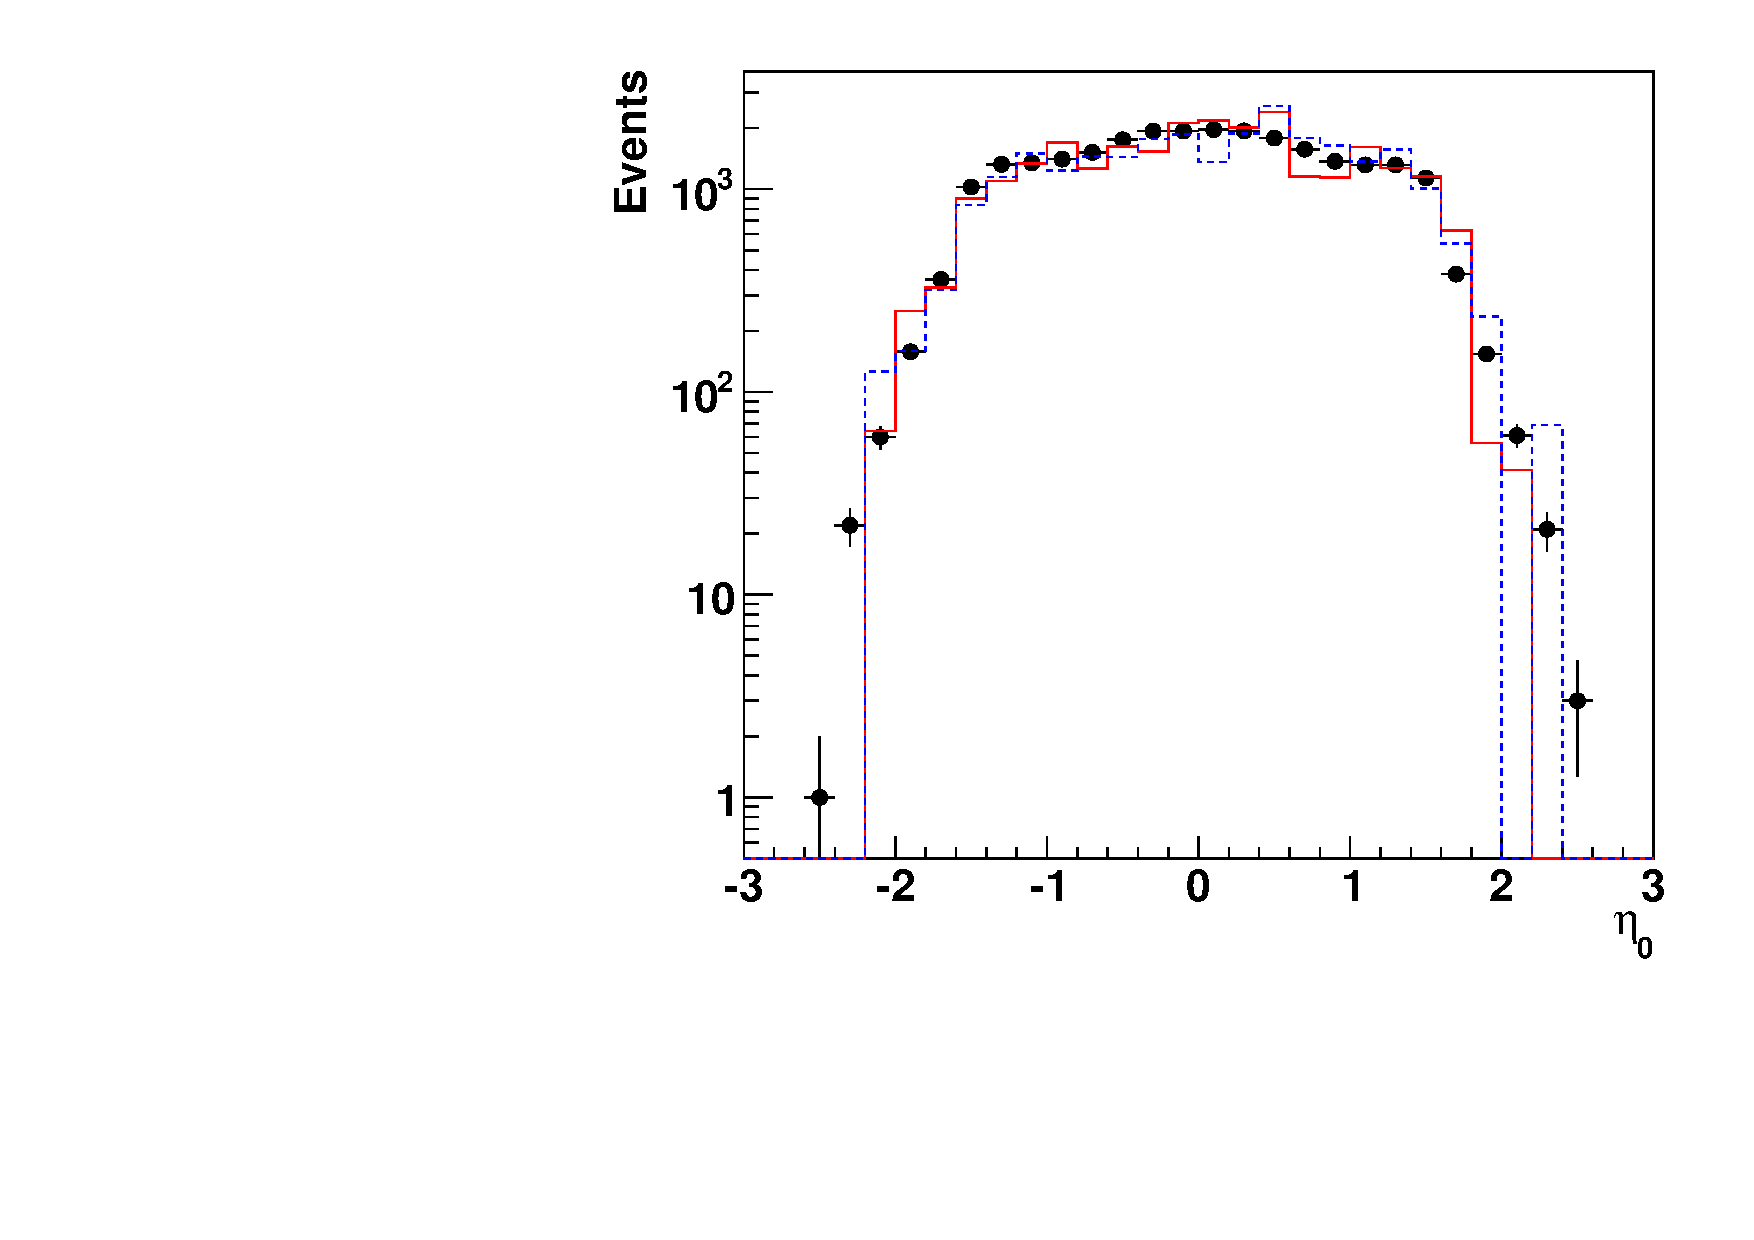
\includegraphics{figs/Data-MC-comparisons/Eta0-VVLowP.pdf}} &
     \resizebox{0.5\linewidth}{!}{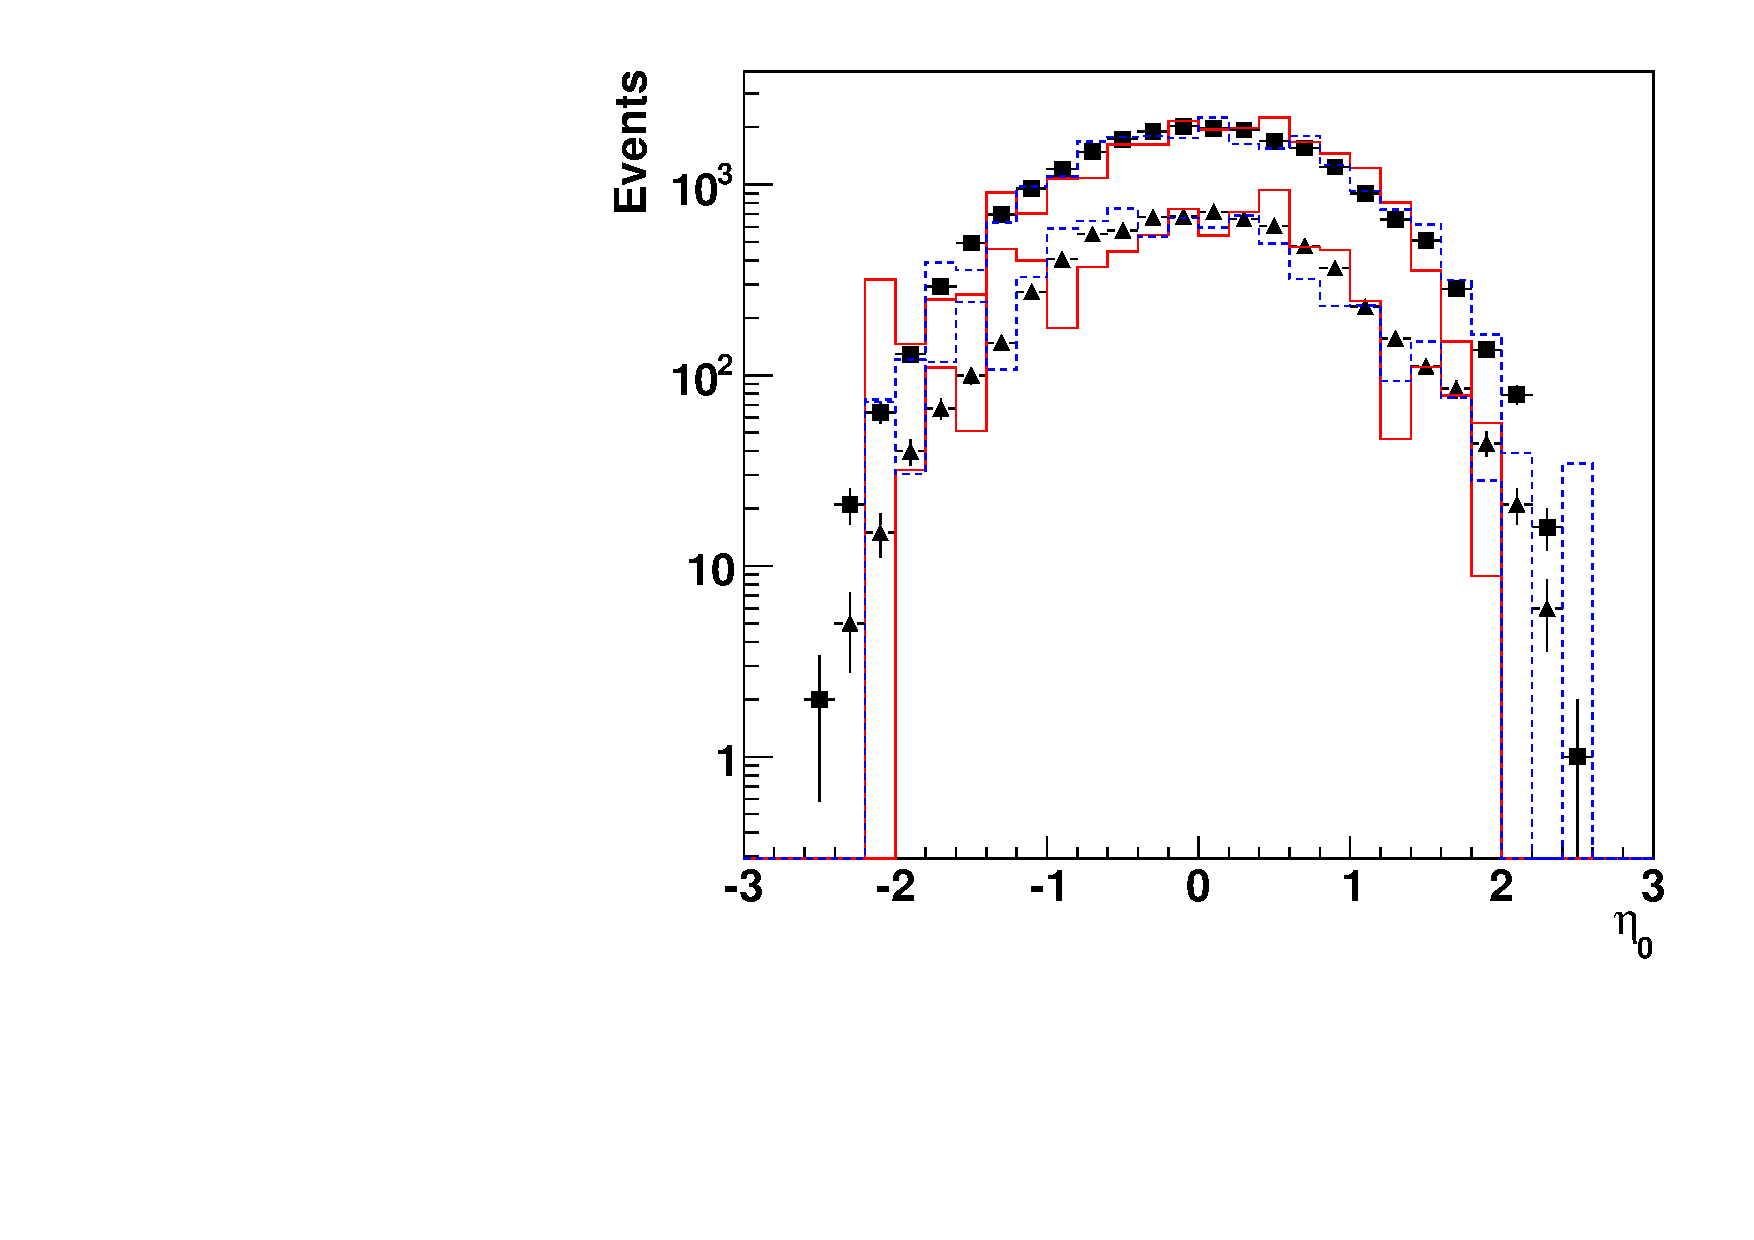
\includegraphics{figs/Data-MC-comparisons/Eta0-VVMiumHigh.pdf}} \\
\end{tabular}
  \caption[Delta Eta Double]{Comparisons between data and Monte Carlo
                     for $\eta$ of the leading jet of low purity (left) and low-high purity (right) 2-tagged events. The MC is normalized to the number of data events in each category. }
  \label{fig:Eta0Double}
\end{figure}


\newpage
\begin{figure}[htb]
\centering
\begin{tabular}{cc}
     \resizebox{0.5\linewidth}{!}{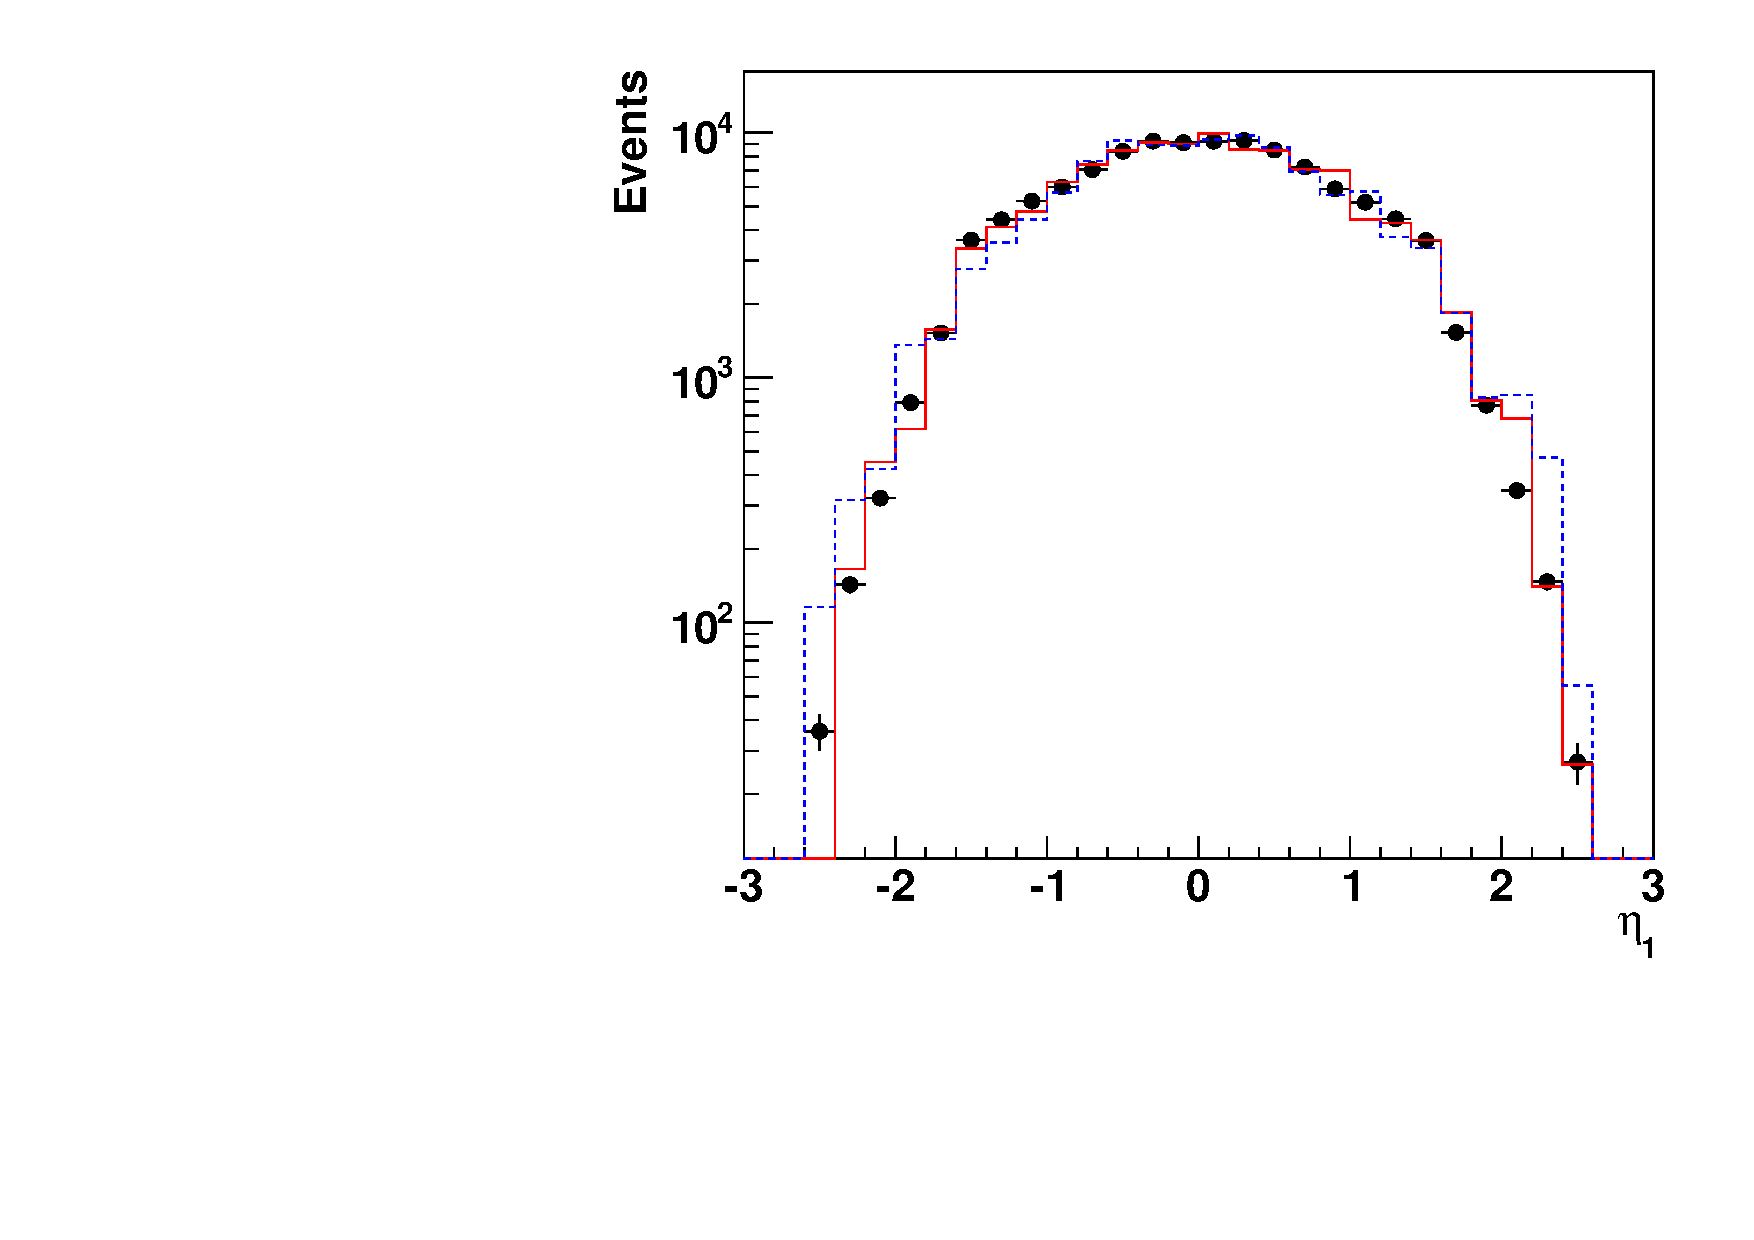
\includegraphics{figs/Data-MC-comparisons/Eta1-qVLowP.pdf}} &
     \resizebox{0.5\linewidth}{!}{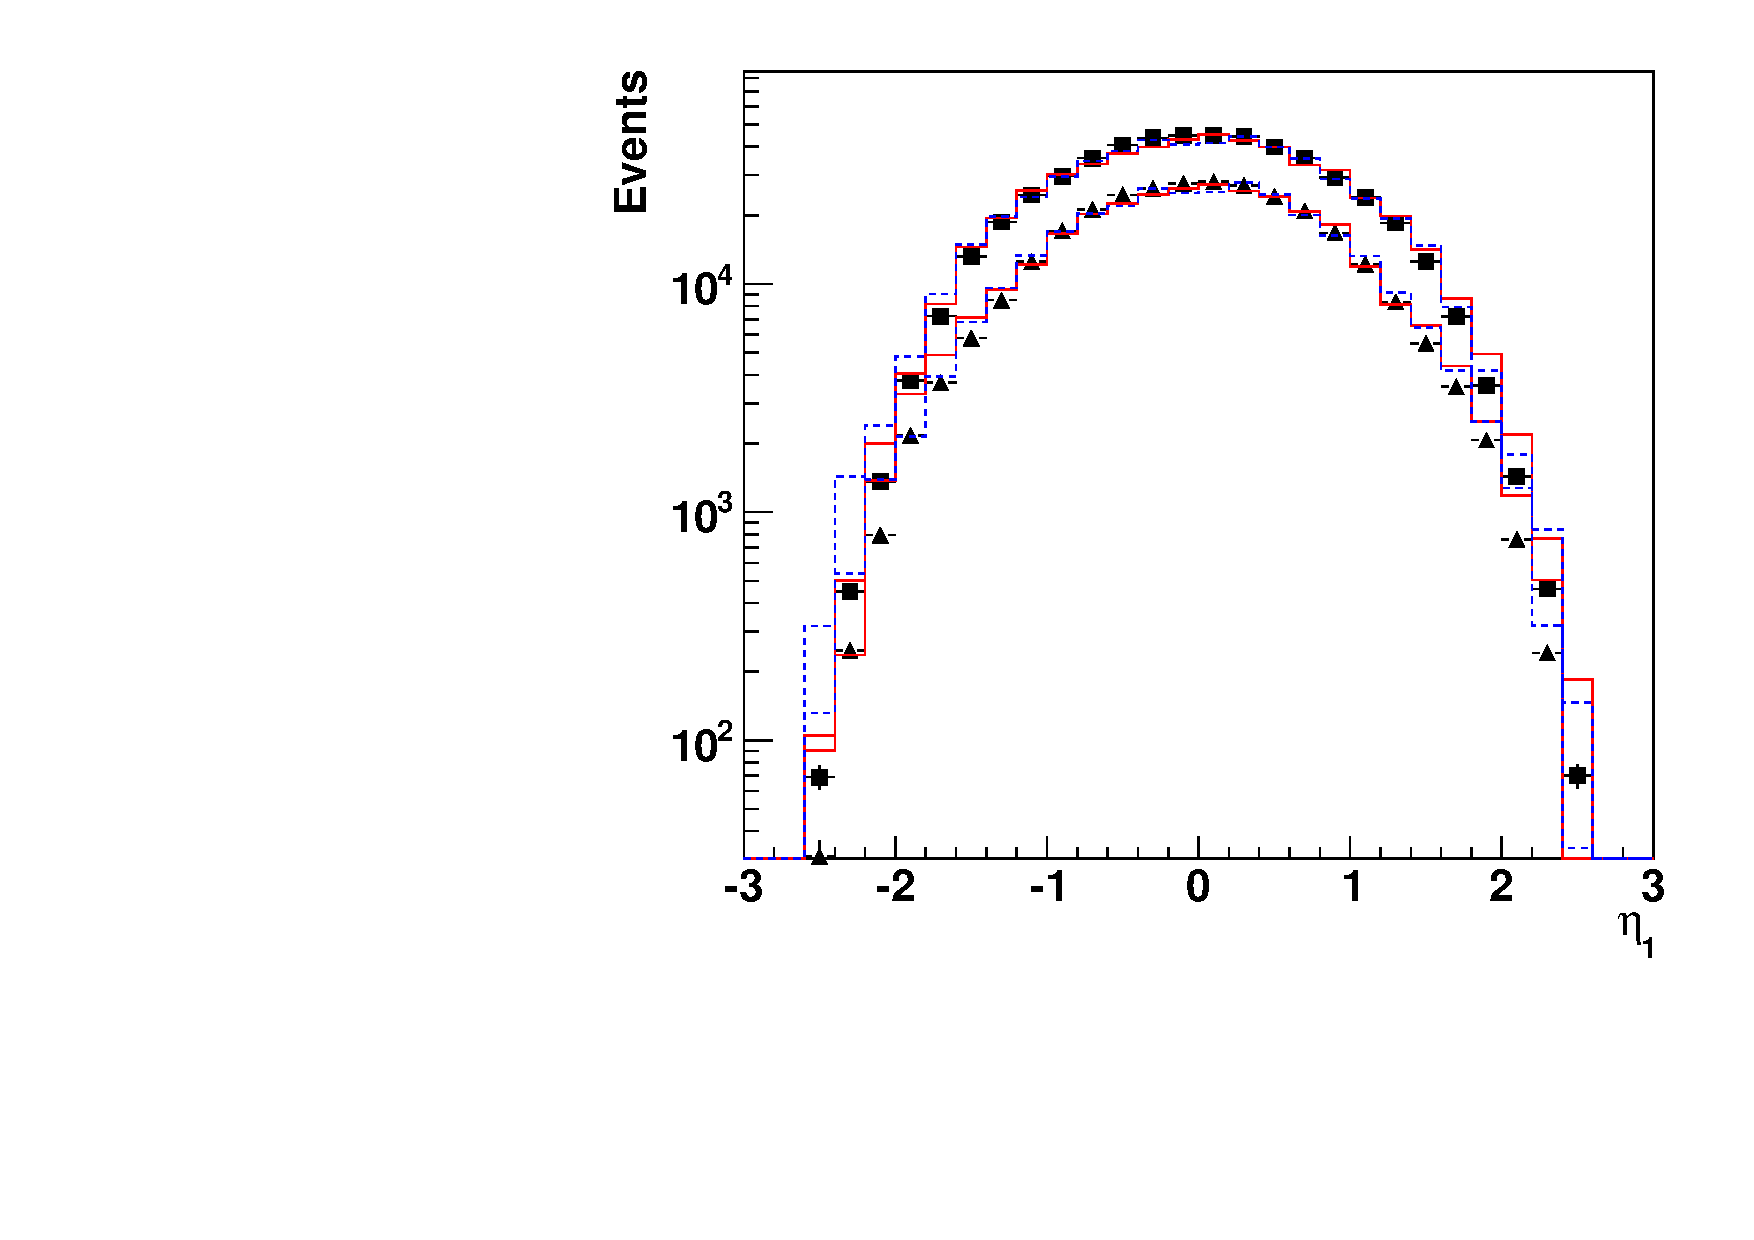
\includegraphics{figs/Data-MC-comparisons/Eta1-qVMiumHigh.pdf}} \\
\end{tabular}
  \caption[PT Single]{Comparisons between data and Monte Carlo
                    for $\eta$ of the second leading jet of low purity (left) and low-high purity (right) 1-tagged events.
	   The MC is normalized to the number of data events in each category. }
  \label{fig:Eta1Single}
\end{figure}

\begin{figure}[htb]
\centering
\begin{tabular}{cc}
     \resizebox{0.5\linewidth}{!}{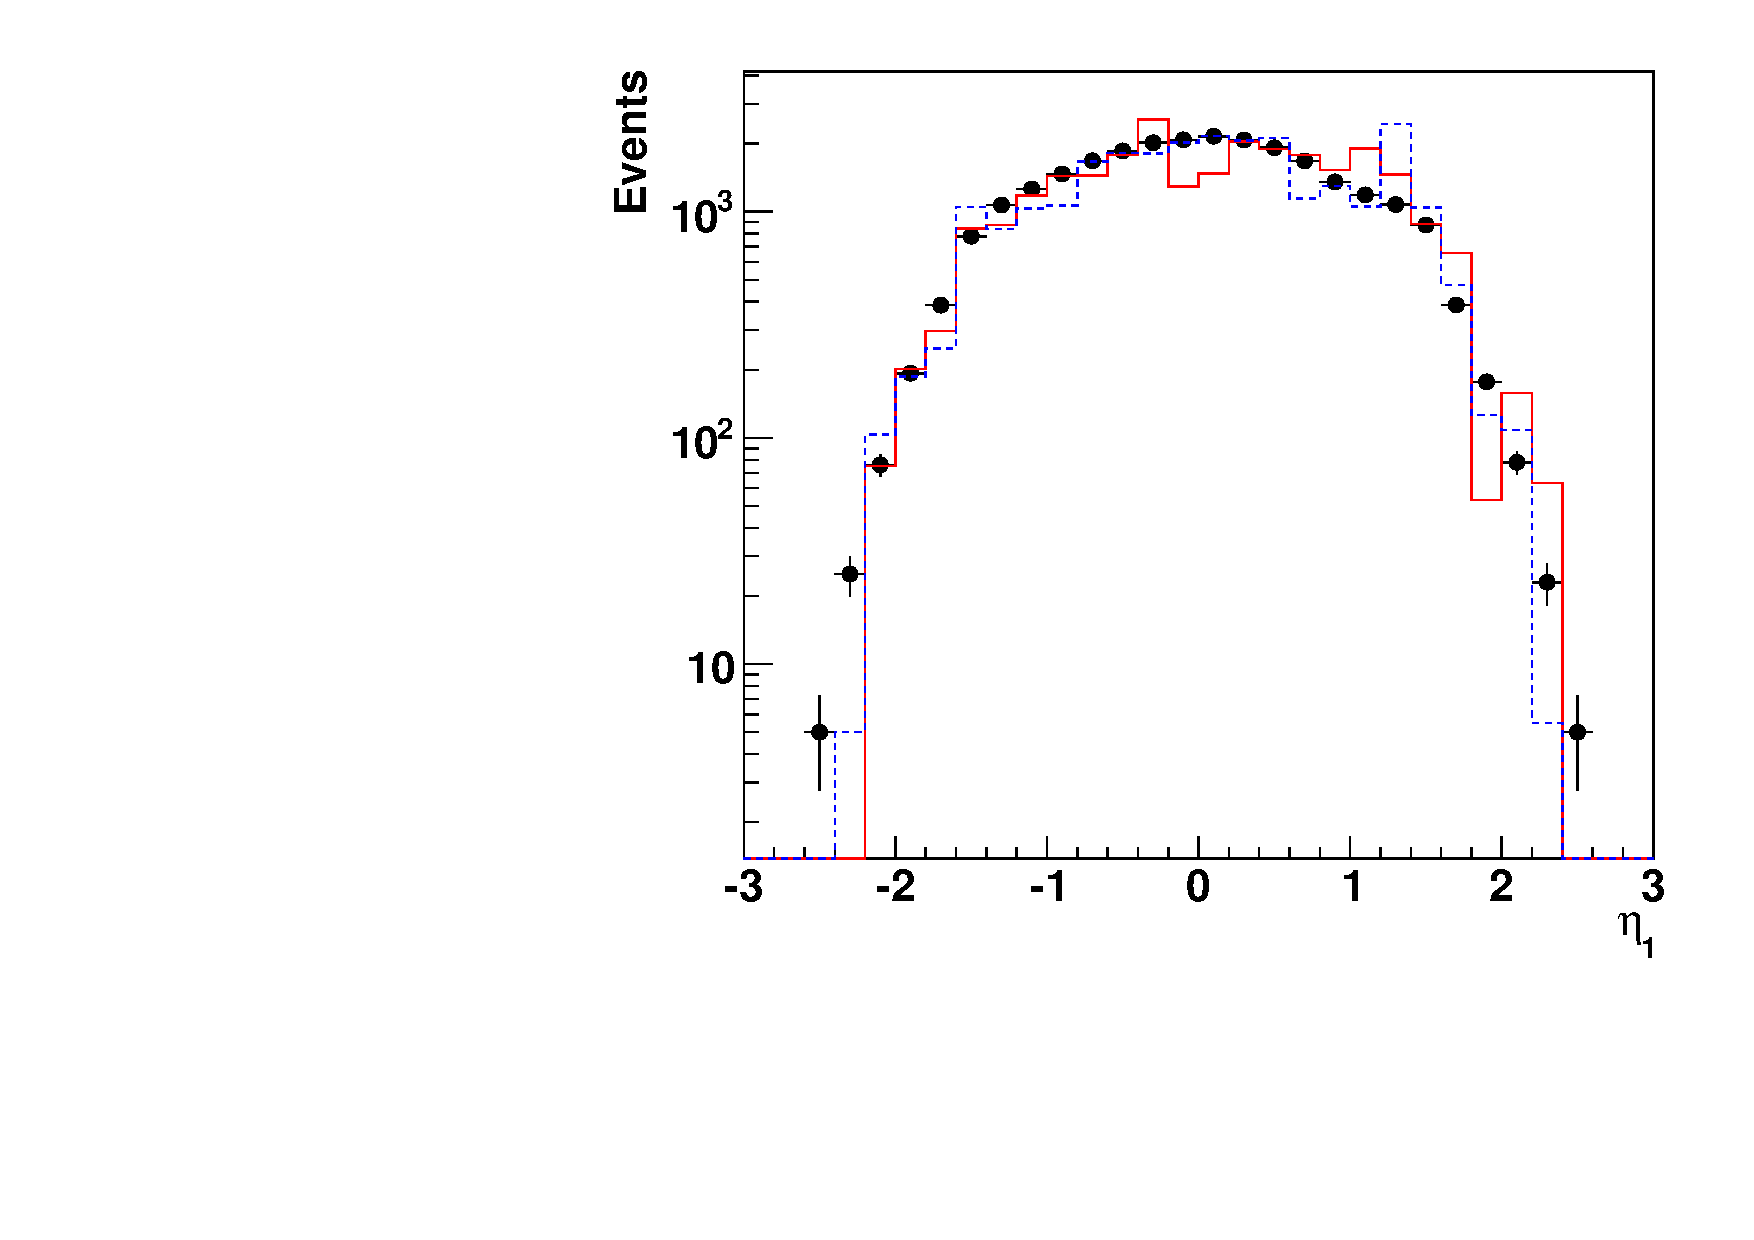
\includegraphics{figs/Data-MC-comparisons/Eta1-VVLowP.pdf}} &
     \resizebox{0.5\linewidth}{!}{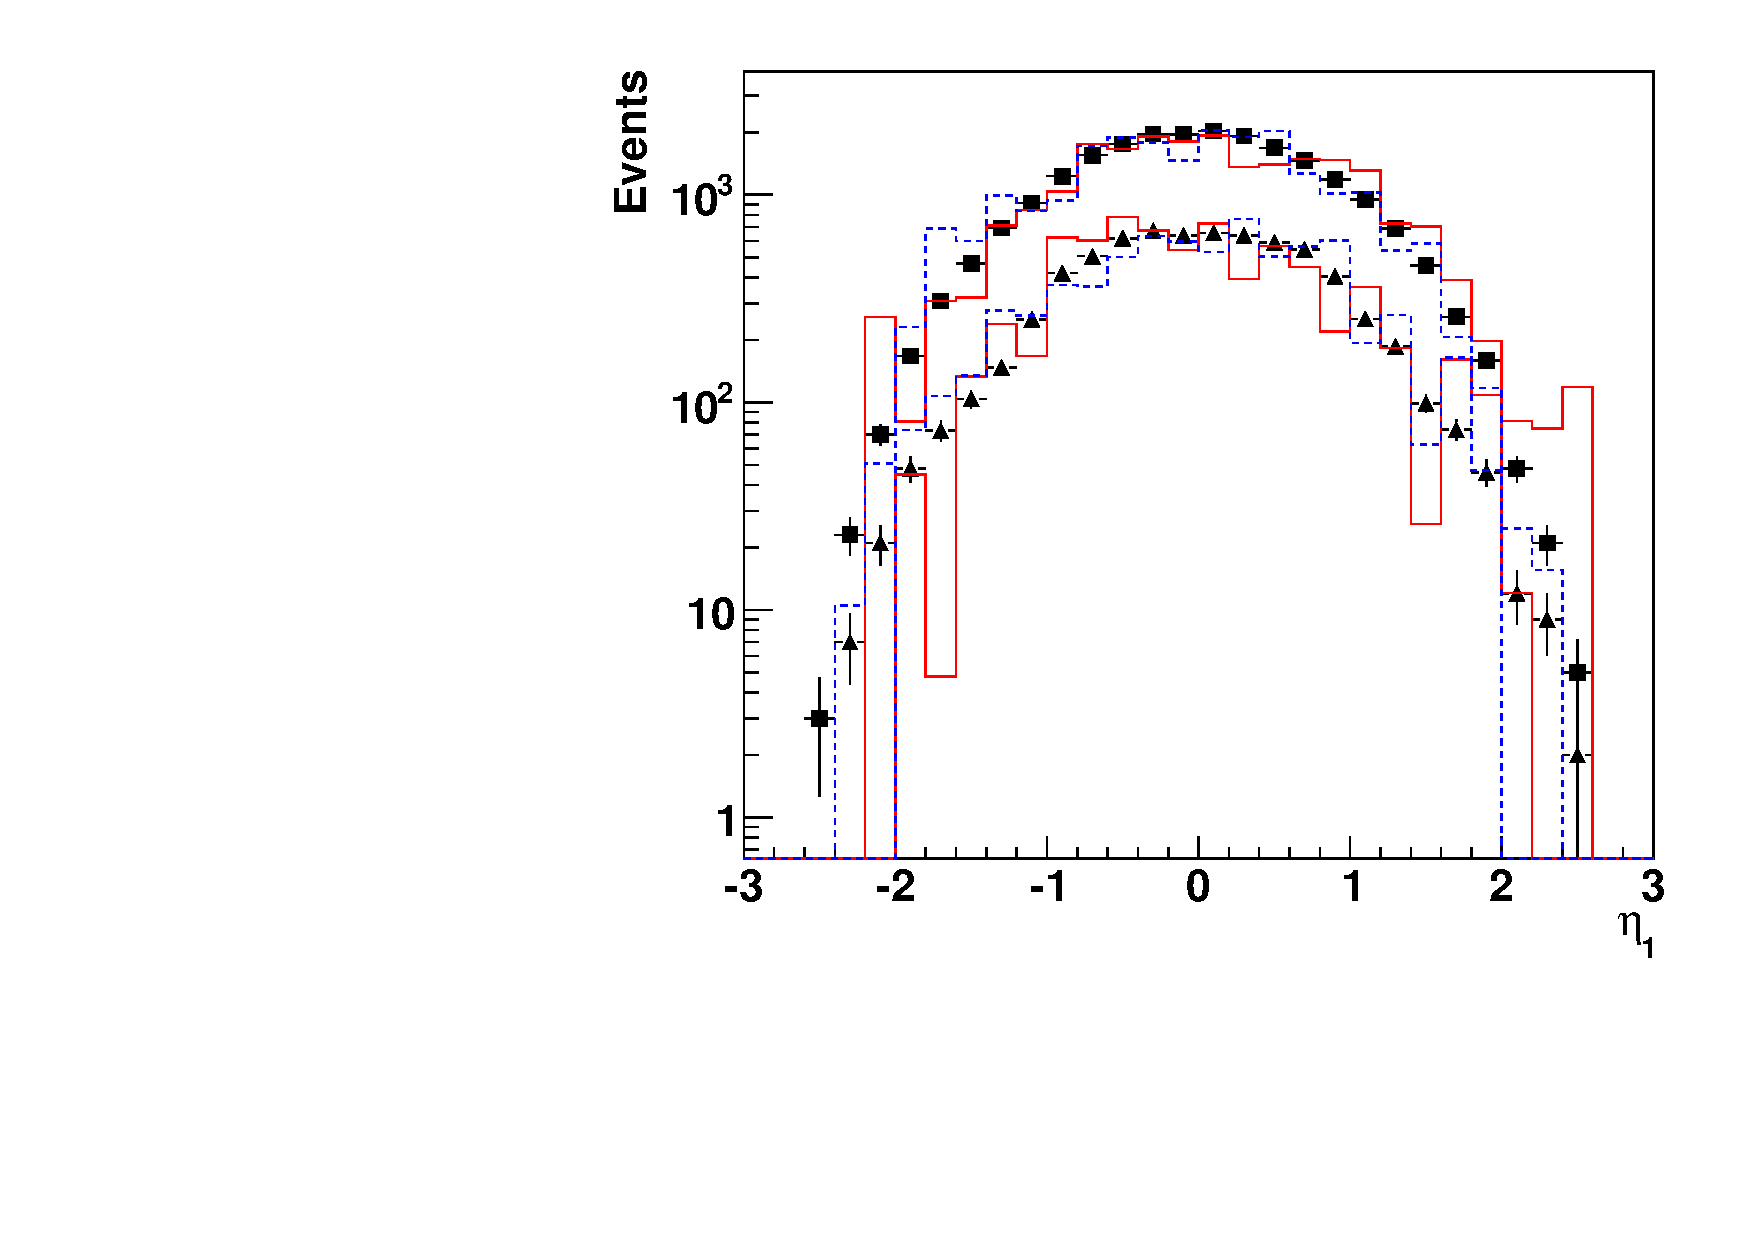
\includegraphics{figs/Data-MC-comparisons/Eta1-VVMiumHigh.pdf}} \\
\end{tabular}
  \caption[Delta Eta Double]{Comparisons between data and Monte Carlo
                     for $\eta$ of the second leading jet of low purity (left) and low-high purity (right) 2-tagged events. The MC is normalized to the number of data events in each category. }
  \label{fig:Eta1Double}
\end{figure}

%\newpage
%\begin{figure}[htb]
%\centering
%\begin{tabular}{cc}
%     \resizebox{0.5\linewidth}{!}{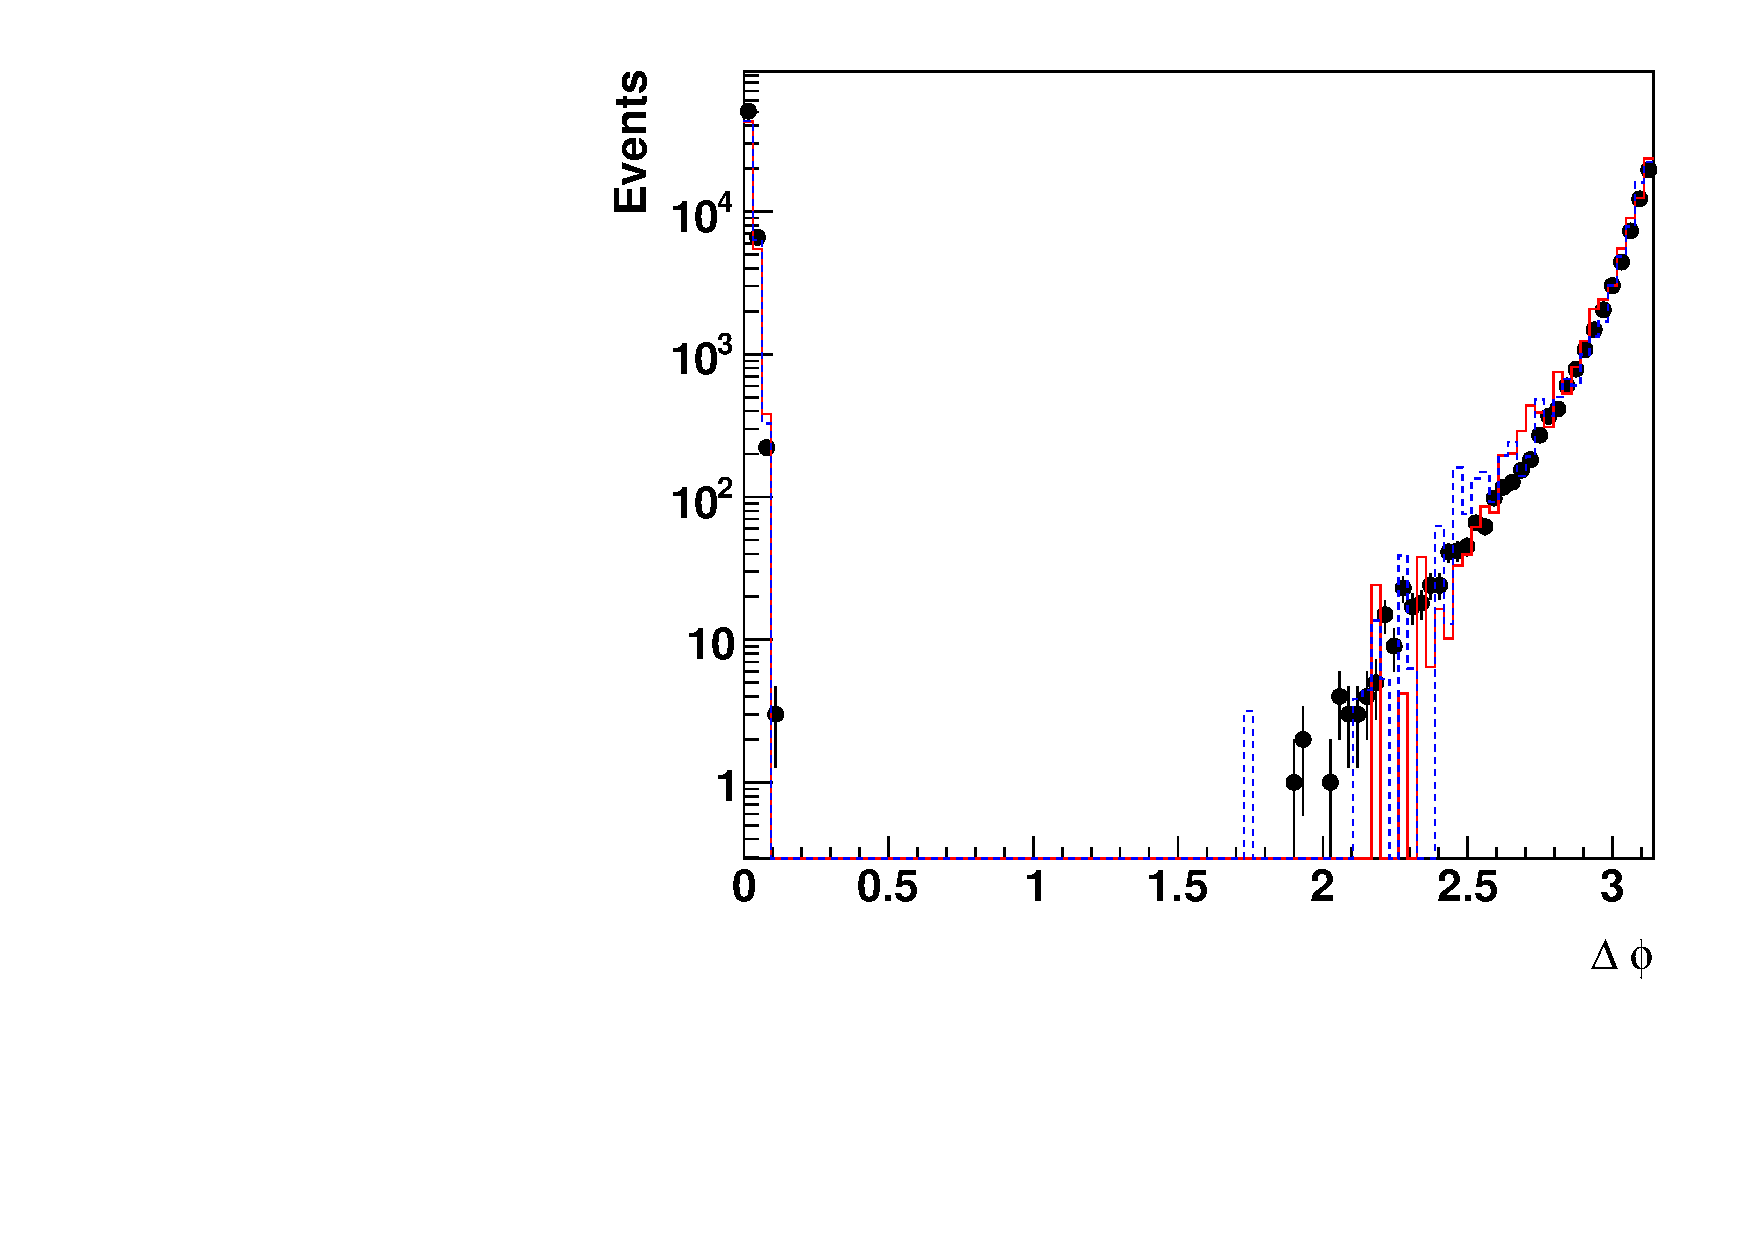
\includegraphics{figs/Data-MC-comparisons/CA8CA8-qVLowP.pdf}} &
%     \resizebox{0.5\linewidth}{!}{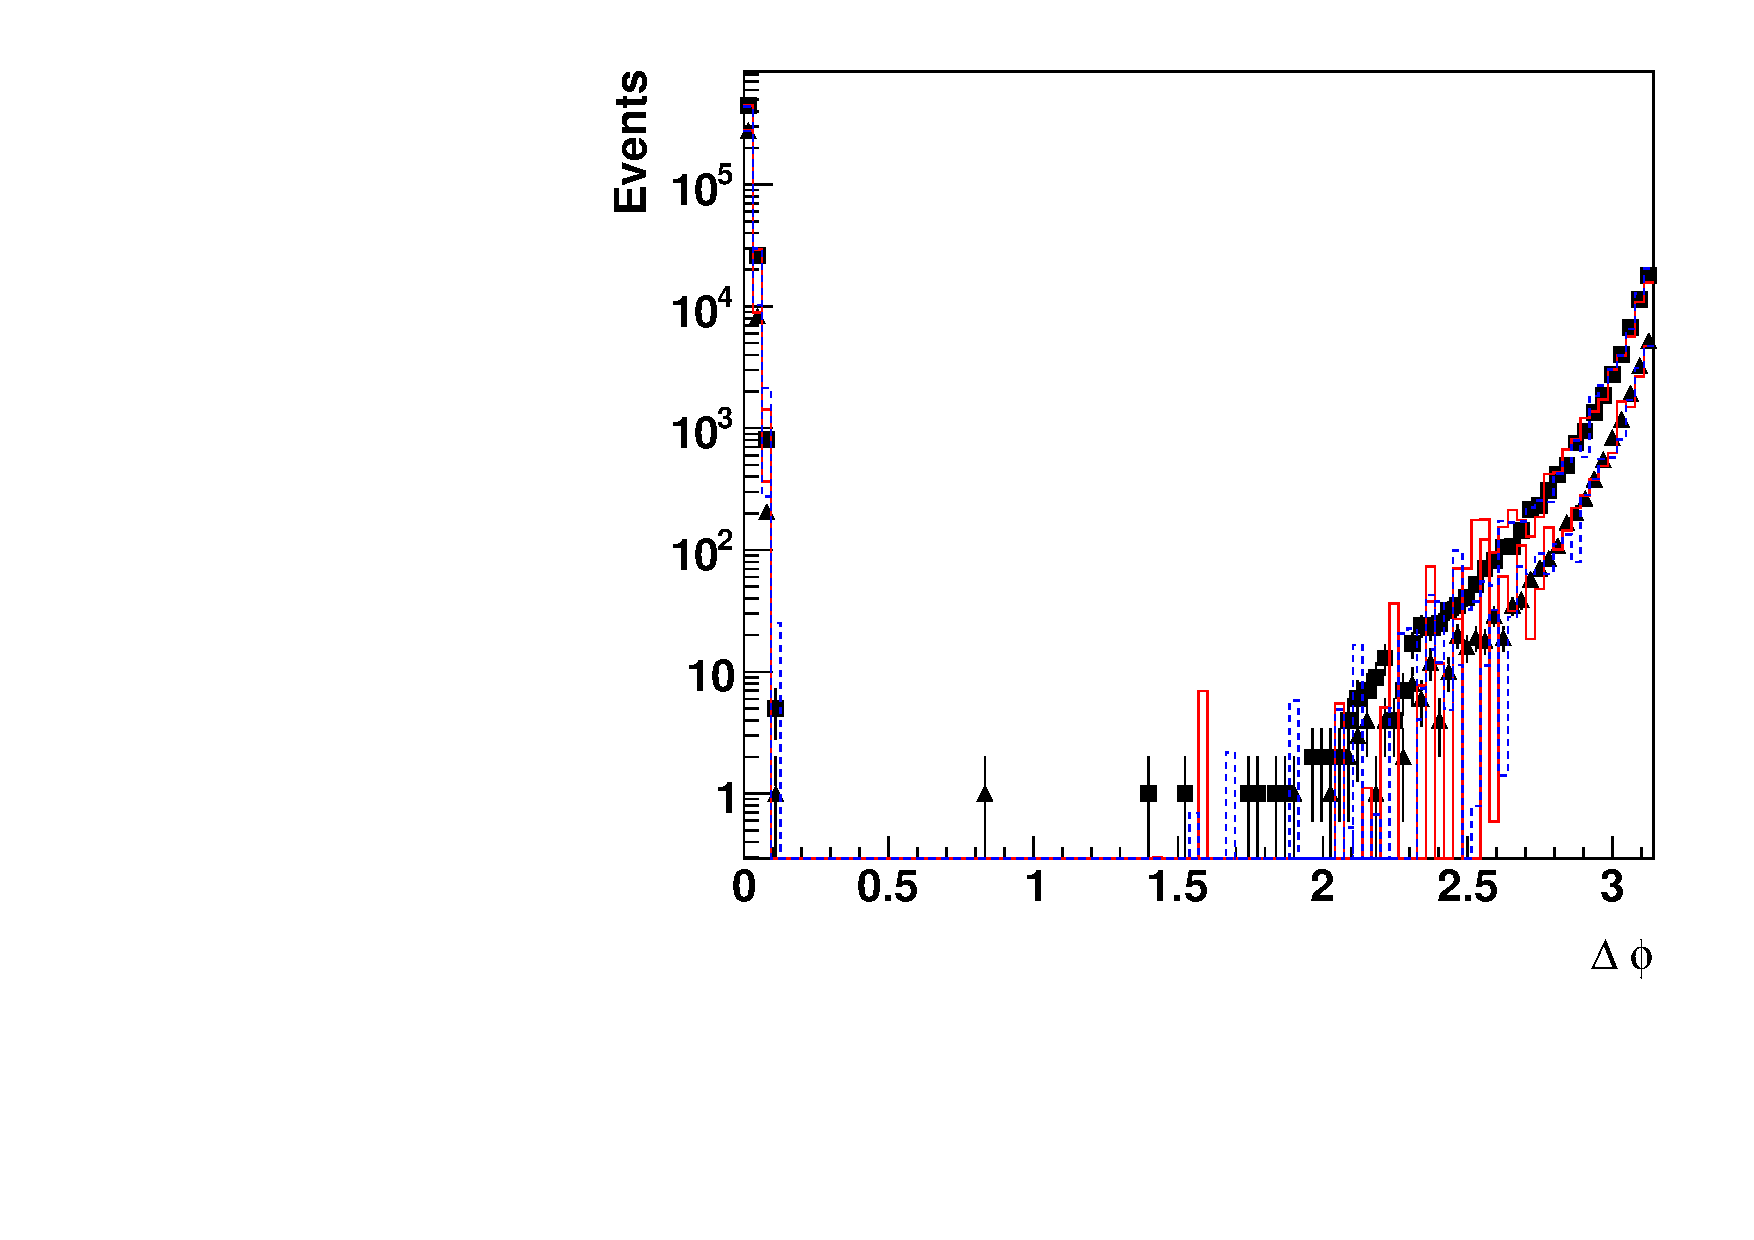
\includegraphics{figs/Data-MC-comparisons/CA8CA8-qVMiumHigh.pdf}} \\
%\end{tabular}
%  \caption[PT Single]{Comparisons between data and Monte Carlo
%                    for $\Delta \phi$ of the leading ungroomed CA8 jet and leading pruned CA8 jet of low purity (left) and low-high purity (right) 1-tagged events.
%	   The MC is normalized to the number of data events in each category. }
%  \label{fig:CA8Single}
%\end{figure}

%\begin{figure}[htb]
%\centering
%\begin{tabular}{cc}
%     \resizebox{0.5\linewidth}{!}{\includegraphics{figs/Data-MC-comparisons/CA8CA8-VVLowP.pdf}} &
%     \resizebox{0.5\linewidth}{!}{\includegraphics{figs/Data-MC-comparisons/CA8CA8-VVMiumHigh.pdf}} \\
%\end{tabular}
%  \caption[PT Single]{Comparisons between data and Monte Carlo
%                    for $\Delta \phi$ of the leading ungroomed CA8 jet and leading pruned CA8 jet of low purity (left) and low-high purity (right) 2-tagged events.
%           The MC is normalized to the number of data events in each category. }
%  \label{fig:CA8Double}
%\end{figure}


\newpage
\begin{figure}[htb]
\centering
\begin{tabular}{cc}
     \resizebox{0.5\linewidth}{!}{\includegraphics{figs/Data-MC-comparisons/lumi19fb_dataMC_ca8jet_norm_mlog.pdf}} &
     \resizebox{0.5\linewidth}{!}{\includegraphics{figs/Data-MC-comparisons/data-qcd-Jet-Tau21.pdf}}\\
\end{tabular}
  \caption[Leading two jets mass]{Comparisons between data and Monte Carlo for
                    mass(left) and $\tau_{21}$(right) of the leading two jets.
	   The MC is normalized to the number of data events in each category.}
  \label{fig:massNsub}
\end{figure}



















\newpage

\begin{figure}[htb]
\centering
\begin{tabular}{cc}
     \resizebox{0.5\linewidth}{!}{\includegraphics{figs/Data-MC-comparisons/npv.pdf}} &
     \resizebox{0.5\linewidth}{!}{\includegraphics{figs/Data-MC-comparisons/npvlog.pdf}} \\
\end{tabular}
  \caption[Leading two jets mass drop]{Comparisons between data and Monte Carlo for
                   number of primary vertice to show the effect on Monte Carlo after pile up reweighting. 
	   The MC is normalized to the number of data events. Plot on the right is the log scale plot. (The plot includes only a subset of the full data sample.)}
  \label{fig:npv}
\end{figure}

\begin{figure}[htb]
\centering
\begin{tabular}{cc}
     \resizebox{0.5\linewidth}{!}{\includegraphics{figs/Data-MC-comparisons/neutralHadronEnergyFraction.pdf}} &
     \resizebox{0.5\linewidth}{!}{\includegraphics{figs/Data-MC-comparisons/neutralHadronEnergyFractionlog.pdf}} \\
\end{tabular}
  \caption[Leading two jets mass drop]{Comparisons between data and Monte Carlo for neutral hadron energy fraction.  
	   The MC is normalized to the number of data events. Plot on the right is the log scale plot. (The plot includes only a subset of the full data sample.)}
  \label{fig:neutralHadronEnergyFraction}
\end{figure}

\newpage

\begin{figure}[htb]
\centering
\begin{tabular}{cc}
     \resizebox{0.5\linewidth}{!}{\includegraphics{figs/Data-MC-comparisons/neutralEmEnergyFraction.pdf}} &
     \resizebox{0.5\linewidth}{!}{\includegraphics{figs/Data-MC-comparisons/neutralEmEnergyFractionlog.pdf}} \\
\end{tabular}
  \caption[Leading two jets mass drop]{Comparisons between data and Monte Carlo for neutral eletromagnetic energy fraction.  
	   The MC is normalized to the number of data events. Plot on the right is the log scale plot. (The plot includes only a subset of the full data sample.)}
  \label{fig:neutralEmEnergyFraction}
\end{figure}

\begin{figure}[htb]
\centering
\begin{tabular}{cc}
     \resizebox{0.5\linewidth}{!}{\includegraphics{figs/Data-MC-comparisons/chargedHadronEnergyFraction.pdf}} &
     \resizebox{0.5\linewidth}{!}{\includegraphics{figs/Data-MC-comparisons/chargedHadronEnergyFractionlog.pdf}} \\
\end{tabular}
  \caption[Leading two jets mass drop]{Comparisons between data and Monte Carlo for charged hadron energy fraction.  
	   The MC is normalized to the number of data events. Plot on the right is the log scale plot. (The plot includes only a subset of the full data sample.)}
  \label{fig:chargedHadronEnergyFraction}
\end{figure}

\newpage


\begin{figure}[htb]
\centering
\begin{tabular}{cc}
     \resizebox{0.5\linewidth}{!}{\includegraphics{figs/Data-MC-comparisons/chargedEmEnergyFraction.pdf}} &
     \resizebox{0.5\linewidth}{!}{\includegraphics{figs/Data-MC-comparisons/chargedEmEnergyFractionlog.pdf}} \\
\end{tabular}
  \caption[Leading two jets mass drop]{Comparisons between data and Monte Carlo for charged eletromagnetic energy fraction.  
	   The MC is normalized to the number of data events. Plot on the right is the log scale plot. (The plot includes only a subset of the full data sample.)}
  \label{fig:chargedEmEnergyFraction}
\end{figure}

\begin{figure}[htb]
\centering
\begin{tabular}{cc}
     \resizebox{0.5\linewidth}{!}{\includegraphics{figs/Data-MC-comparisons/chargedMultiplicity.pdf}} &
     \resizebox{0.5\linewidth}{!}{\includegraphics{figs/Data-MC-comparisons/chargedMultiplicitylog.pdf}} \\
\end{tabular}
  \caption[Leading two jets mass drop]{Comparisons between data and Monte Carlo for charged multiplicity.  
	   The MC is normalized to the number of data events. Plot on the right is the log scale plot. (The plot includes only a subset of the full data sample.)}
  \label{fig:chargedMultiplicity}
\end{figure}

\newpage

\begin{figure}[htb]
\centering
\begin{tabular}{cc}
     \resizebox{0.5\linewidth}{!}{\includegraphics{figs/Data-MC-comparisons/nConstituents.pdf}} &
     \resizebox{0.5\linewidth}{!}{\includegraphics{figs/Data-MC-comparisons/nConstituentslog.pdf}} \\
\end{tabular}
  \caption[Leading two jets mass drop]{Comparisons between data and Monte Carlo for number of constituents.  
	   The MC is normalized to the number of data events. Plot on the right is the log scale plot. (The plot includes only a subset of the full data sample.)}
  \label{fig:nConstituents}
\end{figure}


\begin{figure}[htb]
\centering
\begin{tabular}{cc}
     \resizebox{0.5\linewidth}{!}{\includegraphics{figs/Data-MC-comparisons/muonEnergyFraction.pdf}} &
     \resizebox{0.5\linewidth}{!}{\includegraphics{figs/Data-MC-comparisons/muonEnergyFractionlog.pdf}} \\
\end{tabular}
  \caption[Leading two jets mass drop]{Comparisons between data and Monte Carlo for the muon energy fraction of the leading two jets.  
	   The MC is normalized to the number of data events. Plot on the right is the log scale plot. (The plot includes only a subset of the full data sample.)}
  \label{fig:muonEnergyFraction}
\end{figure}

\newpage


%We find that the QCD MC agrees with data, although not perfect.
%For the dijet kinematics shown in Fig~\ref{fig:mjj},\ref{fig:dy},\ref{fig:dphi},\ref{fig:metSumPt},\ref{fig:jet1-pt},\ref{fig:jet2-pt},\ref{fig:eta of leading jet} and \ref{fig:eta of second leading jet}, we observe better agreement of Pythia6 $Z2*$ than Herwig++.
%For the jet substructure variables shown in Fig~\ref{fig:mass of leading two jets},\ref{fig:mass drop of leading two jets} and \ref{fig:subjet dR of leading two jets}, we observe that Herwig++ is better than Pythia $Z2*$.  
%In summary, Pythia6 $Z2*$ is more accurate at modelling the dijet kinematics,
%while Herwig++ models better the jet substructure.
We find that the QCD MC agrees with data, although not perfect.
For the dijet kinematics and also the jet substruture variables, we observe about the same agreement of Pythia6 $Z2*$ and Herwig++. 
For this analysis, we chose to model the background shape from the data itself
(as described below)
and depend on QCD MC only to provide us guidance and a cross check.

Fig~\ref{fig:dphiSingle}, Fig~\ref{fig:dphiDouble} and Fig~\ref{fig:metSumPtSingle} are particulariy useful to identify jets from calorimenter noise which would show up at low values of $\Delta\phi$ and high values of $E_{T}^{miss}/\sum E_{T}$. No enhencement in this region is observed which gives confidence that the applied noise filter cleaning and jet ID cuts leave no noise contamination within the two leading jets.

%Fig~\ref{fig:CA8Single} and Fig~\ref{fig:CA8Double} show the $\Delta \phi$ between the leading ungroomed CA8 jet and leading pruned CA8 jet.

%\begin{table}[htb]
%\begin{center}
%\begin{tabular}{|p{2.5cm}|p{2.5cm}|p{2.5cm}|p{2.5cm}|p{2.5cm}|}
%\begin{tabular}{|c|c|c|c|}
%\hline
%Categories & $\Delta \phi < 0.5(\%) $  & $0.5 < \Delta\phi < 2.0 (\%)$ & $2.0 < \Delta\phi (\%)$ \\
%\hline
%low purity 1-tag& 51.067 & 0.003 & 48.930 \\
%medium purity 1-tag&  90.458 & 0.002 & 9.541 \\
%high purity 1-tag & 95.156 & 0.001 & 4.844\\
%low purity 2-tag &  89.332 & 0.004 & 10.664 \\
%medium purity 2-tag& 90.636 & 0 & 9.363\\
%high purity 2-tag &  92.585 & 0 & 7.415\\
%\hline
%\end{tabular}
%\end{center}
%\caption{The ratio of the leading ungroomed CA8 jet matching to the leading pruned CA8 jet in different categories.}
%\label{table:matching}
%\end{table}


%Table~\ref{table:matching} shows the matching of the leading ungroomed CA8 jet and the leading pruned CA8 jet. 
%In the case of  $\Delta \phi<0.5$, the leading ungroomed CA8 jet  and leading pruned CA8 jet match.
%In the case of  $0.5 < \Delta \phi<2.0$, the leading ungroomed CA8 jet  and leading pruned CA8 jet don't match at all.
%In the case of  $\Delta \phi > 2.0$, the leading two jets are swapped and the leading ungroomed CA8 jet matches to the second leading pruned CA8 jet.

%Therefore there is no significant impact on the analyis from the fact that we use the leading two ungroomed CA8 jets to reconstruct the dijet mass while using the leading two pruned CA8 jets for W/Z-tagging of events.

Fig~\ref{fig:npv} shows the number of primary vertices distribution after pile up reweighting on the MC. 
Fig~\ref{fig:neutralHadronEnergyFraction}, Fig~\ref{fig:neutralEmEnergyFraction}, Fig~\ref{fig:chargedHadronEnergyFraction}, Fig~\ref{fig:chargedEmEnergyFraction}, Fig~\ref{fig:chargedMultiplicity} and Fig~\ref{fig:nConstituents} show the jet ID variable distribution after the event selection, and Fig~\ref{fig:muonEnergyFraction}, the muon energy faction of the leading two jets.

\clearpage

%\clearpage
\section{W-tagging scale factor}

We derive the scale factor for the $\tau 2/\tau 1$ W tagger, in both the tight and loose regions, by
comparing its efficiency in semileptonic $t\overline{t}$ events, both
in data and mote carlo. We isolate the W candidates with kinematic
cuts. We consider only muon events. We then apply the tagger and require the W mass to be within
$70$ and $100~\GeVcc$.

In Monte Carlo, we attempt to match the CA8 jets to real Ws by
requiring that the daughters of a hadronic W from the particle generator lie within a
cone of $\Delta R < 0.3$ of a jet's subjets. Jets that meet this
requirement are ''matched'' jets. We can then classify all W
candidates in the following ways:
\begin{enumerate}
\item Matched W jets which pass the tight $\tau 2/\tau 1$ cut.
\item Matched W jets which pass the loose $\tau 2/\tau 1$ cut.
\item Matched W jets which fail both $\tau 2/\tau 1$ cuts.
\item Unmatched W jets which pass the tight $\tau 2/\tau 1$ cut.
\item Unmatched W jets which pass the loose $\tau 2/\tau 1$ cut.
\item Unmatched W jets which fail both $\tau 2/\tau 1$ cuts.
\end{enumerate}
The efficiency for either tight or loose can be extracted by counting the number of matched
W jets in that region and dividing by the total number of
matched W jets.

We derive the efficiency in data by simultaneously fitting the
W mass distributions of the events in the tight, loose and failed events. The general shapes of the distributions are taken from MC. The efficiencies are explicit fit parameters which relate the normalizations of categories category. We must also take into account small background contributions from non-$t\overline{t}$ sources. These contributions are also parametrized as shapes and included in the fit.

\subsection{Fit to monte carlo}

We first find the PDFs associated with each of the event categories
above by fitting their distributions from the Monte Carlo, 
as follows:
\begin{itemize}
\item {\bf Tight, Matched Jets} We fit the tight matched events with the sum of two gaussians.
\item {\bf Loose, Matched Jets} We fir the loose matched events with a sum of the double-gaussian found in the tight selection and an exponential.
\item {\bf Failed, Matched Jets} We fit failed matched events with an exponential.
\item {\bf Tight, Unatched Jets} We fit tight unmatched events with the sum of a gaussian and a linear function with positive slope.
\item {\bf Loose, Unatched Jets} We fit loose unmatched events with a gaussian.
\item {\bf Failed, Unatched Jets} We fit failed unmatched events with an exponential.
\item {\bf Backgrounds} All backgrounds are fit with gaussians in the tight and loose regions, and an exponential in the failed region. These shapes are added to the respective unmatched shapes to derive a total non-matched shape.
\end{itemize}
Fits to matched and unmatched distributions are shown in figures \ref{fig:fitsmatched} and \ref{fig:fitsunmatched}.
%\includegraphics[width=0.35\textwidth]{figs/limits/brazilianFlag_qW_high_purity.pdf}%
\begin{figure}[h!]
\centering
                \includegraphics[width=0.32\textwidth]{EXO-12-024/figs/WtagSF/MT.pdf}
                \includegraphics[width=0.32\textwidth]{EXO-12-024/figs/WtagSF/ML.pdf}
                \includegraphics[width=0.32\textwidth]{EXO-12-024/figs/WtagSF/MF.pdf}
\caption{Fits to matched $t\overline{t}$ distributions. Left: tight region. Center: loose region. Right: failed events.}\label{fig:fitsmatched}
\end{figure}

\begin{figure}[h!]
\centering
                \includegraphics[width=0.32\textwidth]{EXO-12-024/figs/WtagSF/UT.pdf}
                \includegraphics[width=0.32\textwidth]{EXO-12-024/figs/WtagSF/UL.pdf}
                \includegraphics[width=0.32\textwidth]{EXO-12-024/figs/WtagSF/UF.pdf}
\caption{Fits to unmatched $t\overline{t}$ distributions. Left: tight region. Center: loose region. Right: failed events.}\label{fig:fitsunmatched}
\end{figure}

\subsubsection{Fits to data}
We fit the above shapes to the data. The following parameters are kept constant, with their values taken form the MC fits described in the previous section:
\begin{enumerate}
\item In the unmatched and background distrubtions
	\begin{enumerate}
	\item The relative normalization of the gaussian and linear components of the tight, unmatched shape.
	\item The position of the gaussian peak in the loose, unmatched distribution is fixed.
	\item The means and standard deviations, as well as the decay coefficients of all backgrounds are fixed, but their normalizations are not.
	\end{enumerate}
\item In the matched distributions
        \begin{enumerate}
	\item The relative normalization of the two gaussians in the tight region is fixed.
	\item The relative position (as a multiplier) of the two gaussian peaks is fixed.
	\item The relative normalization of the exponential and double-gaussian shapes in the loose region is fixed.
        \end{enumerate}
\end{enumerate}

All other parameters are allowed to float. All other normalizations are parametrized in terms of the efficiency. The results of the fits to data are shown in figure \ref{fig:datafits}. As a consistency check, the same proceedure is applied to the MC distribution. The result of that fit is shown in figure \ref{fig:mcfits}.
\begin{figure}[h!]
\centering
        \includegraphics[width=0.49\textwidth]{EXO-12-024/figs/WtagSF/MCTIGHT.pdf}
	\includegraphics[width=0.49\textwidth]{EXO-12-024/figs/WtagSF/MCLOOSE.pdf}
        \caption{Distributions from data of $W$ mass in the tight (left) and loose (right) $\tau_2/\tau_1$ regions, and resulting fits.}\label{fig:datafits}
\end{figure}
\begin{figure}[h!]
\centering
        \includegraphics[width=0.49\textwidth]{EXO-12-024/figs/WtagSF/TIGHT.pdf}
	\includegraphics[width=0.49\textwidth]{EXO-12-024/figs/WtagSF/LOOSE.pdf}
        \caption{Distributions from MC of $W$ mass in the tight (left) and loose (right) $\tau_2/\tau_1$ regions, and resulting fits.}\label{fig:mcfits}
\end{figure}

More details on the fitting procedure and the $t\overline{t}$ selection can be found in the appendix of this note.

\subsection{Scale factor measurement}
We measure the scale factor of the $\tau 2/\tau 1$ cut efficiency and that of the W mass window $70$ to $100\GeVcc$ efficiency. We find that the total scale factor for the two cuts is $0.860 \pm 0.065$ in the tight region and $138.5 \pm 75.2$ in the loose region.

\subsubsection{Related systematics}
The errors in the scale factors are found from the fitting errors and systematic errors from the choice of fixed parameters. Each fixed parameter found in MC is varied by its fitting error and used to generate toy MC to which the fitting proceedure is applied. The resulting offset is taken to be the systematic error from this fixed parameter. In addition, when the efficiency from a fit to MC differs with that from MC truth information, we take the difference to be an additional systematic. 
Additional systematic uncertainties on the W-tagging efficiency related to detector effects are discussed in the systematics section of this note.
\clearpage

%\section{Signal efficiency}
\label{sec:signal}

We search for several models of heavy resonances decaying to
a W or Z boson on one side, and a Higgs on the other, where both bosons 
decay to quarks producing merged jet.  This analysis is focused on two
channels:
\begin{itemize}
\item \HbbVqq, and
\item \HwwVqq
\end{itemize}
As previously discussed, we use one V-tagging and two Higgs tagging algorithms
to identify such events.  After subdividing the events according to 
high purity and low purity tags, we end up with five distinct categories,
as shown in Table~\ref{table:categories}.

In this section, we discuss various issues related to the evaluation
of the signal efficiency.

% For Higgs decays to \bbbar, we use a pruned jet mass and also b
% tagging to discriminate higgs jet from QCD jets and jets from the
% fully merged hadronically decaying top quark.
% Fig.~\ref{fig:JetMassTagging} shows the pruned jet mass distribution for
% Higgs jet, $\Zqq$ jet, hadronic top jets and QCD jets.


%HbbZqqfigs/Signal



%% &&& Plot:  the pruned jet mass of Higgs Jet and QCD jet , Z jet, top jet? in one plot. 

%% &&& Plot:  tau42 for Higgs Jet , Z jets, WJets, top jet, in one plot. leptonic top jet ?


%The pruned jet mass and jet $\tau_{21}$ distributions in signal MC, data and background MC are shown in Fig.~\ref{fig:taggingvariables}.



\subsection{Cross-talk between the Higgs decay channels}
\label{sec:cross-talk}

In order to combine events from all categories into a single joint
likelihood, the categories must be mutually exclusive.  However, a
cross-talk between the Higgs channels is neverthelss possible: for
example, $\Hbb$ tagger can identify other two-prong Higgs decay modes
like ${\rm H\to gg}$, $H \to \tau \tau$, or ${\rm H \to c\bar{c}}$,
although this kind of `false positive' tag happens only rarely (the
efficiency is $\lesssim 6~\%$).  Similarly, events from two-prong
Higgs decay channels can also pass the $\tau_{42}$ cut in the
$\Hww$ selection.  In this case, the channel $\Hbb$, because of its large
branching ratio, contributes a non-negligible number of events to the
sample of 4q tags.  This effect is illustrated by
Fig.~\ref{fig:HiggsTau42}, where it can be seen that most of the
low-$\tau_{42}$ tail of the $\Hbb$ curve will be below the cut value of 0.55.
\begin{figure}[htb]
\centering
\begin{tabular}{cc}
%     \resizebox{0.5\linewidth}{!}{\includegraphics{HqqqqZqqfigs/N-subjettiness/Tau421TeVPre.pdf}} &
     \resizebox{0.7\linewidth}{!}{\includegraphics{EXO-14-009/HqqqqZqqfigs/cross-talk/cross-talk.pdf}} \\
\end{tabular}
\caption{ Comparison of $\tau_{42}$ distribution for H(ww$\to qqqq$), H(gg), H(bb), H(cc), H($\tau\tau$) channels.
All curves are drawn for Higgs jets after pruned jet mass cut, and also normalized with 
respective branching ratios.}
\label{fig:HiggsTau42}
\end{figure}
 

%\newpage
%\section{Hbb HWW and other Channels}
%\label{sec:contamination}

Table~\ref{table:HbbHww} provides an overview of the cross-talk
between the various channels.  The Higgs branching ratios correspond
to the Higgs mass of 125~\GeVcc. 
 For ${\rm H \to WW^* \to 4q }$,
the branching ratio of the hadronic decay of (real) W boson is already 
included, so that the final state is four quarks.
%
The table is normalized to 100,000 standard model Higgs
bosons, and the numbers in the
table show the number of Higgs decays that pass the tagger for each
channel, with the branching ratio taken into account.  For example, 
let us consider ${\rm H \to c\bar{c}}$ channel.  At the Z' resonance
mass of 1~\TeVcc, out of 100,000 Higgs decays,  104 events 
are tagged by the $\Hbb$ tagger  
and  82  pass $\Hww$ tagger but fail $\Hbb$ tagger.
For ${\rm H \to ZZ}$ decays, we take its tagging efficiency the same 
as $\Hww$ signals. So the number of ${\rm H \to ZZ}$ to pass $\Hbb$ and 
$\Hww$ tagger is estimated by 
efficiency of $\Hww$ signal times 
 BR(Hzz)*BR(Zqq)*BR(Zqq) divided by BR(Hww)*BR(Wqq)*BR(Wqq). 

From Table~\ref{table:HbbHww}, it can be seen that for various signal 
resonance masses, the contribution of other decay channels to the 
sample of $\Hbb$ tags never exceeds 6\%. We will assign additional systematics
for the cross-talk.  
%This is smaller than several
%of the systematic uncertainties, and we do not correct for it.

%And also the ratio of other signals, i.e. Htt, Hgg, Hcc to pass $\Hww$
%tagger, is around 14\% of $\Hww$ plus $\Hbb$ decay modes.
%Their contamination in data should be very tiny.  

Since the $\Hbb$ tagger has significantly lower background than $\Hww$,
it takes precedence in selecting events: we first identify the
events that pass the $\Hbb$ tagger, and only if they fail,  we
test them for the presence of the $\Hww$ tag.  

%As a consequence
%of such cascading selection, we divide the signal events
%into three categories:
%\begin{enumerate}
%\item $\Hbb$ decays reconstructed by the $\Hbb$ tagger
%\item $\Hbb$ decays that failed the $\Hbb$ tagger, but pass $\Hww$ tagger
%\item $\Hww$ events that pass $\Hww$ tagger.
%\end{enumerate}
%Each of these categories must be treated as a separate signal
%component in the multi-channel joint likelihood.
%, with the Higgs
%branching ratios as the nuisance parameters.

The effect of the $\Hbb$ tagger veto on the $\Hww$ tagged dijet 
mass distribution
background (data) is shown in Appendix~\ref{appendix:crosstalkData}.
%The fraction of $\Hww$ tags which are also $\Hbb$ tags are small,
%about 3\%, and it is roughly a slowly
% rising slope as a function of the dijet
%invariant mass.


\begin{table}[htbp]
\begin{center}
\caption{Number of Higgs jets falls into two exclusive categories, assuming we have 100,000 SM Higgs (125 GeV) decays to all channels.
$\Hzz$ signals are estimated by its branching ratio times the efficiency of $\Hww$ signals divied by the branching ratio of $\Hww$ channel. }
\begin{tabular}{|l|r|r|r|r|}
\hline
%& \multicolumn{1}{l|}{Branching ratio (\%)} & \multicolumn{1}{l|}{Pass $\Hbb$} & \multicolumn{1}{l|}{Pass $\Hww$} & \multicolumn{2}{l|}{Fail $\Hbb$, pass $\Hww$} \\ \hline
& Branching  & Pass       & Fail $\Hbb$, pass \\
& ratio (\%) & $\Hbb$  &   $\Hww$ \\ 
\hline
1.5 TeV  & & & \\
$\Hbb$ & 57.70 & 11444 &  755 \\ %\hline
$\Hww$ & 9.94 & 228 & 1916 \\ % \hline
$\Hzz$ & 1.30 & 29 & 250 \\ % \hline
${\rm H\to c\bar{c}}$ & 3.00 & 121 & 88 \\ %\hline
${\rm H\to} \tau \tau$ & 6.30 & 12  & 57 \\ %\hline
${\rm H\to gg}$ & 10.00 & 69 & 174 \\ %\hline
% & \multicolumn{1}{l|}{} & \multicolumn{1}{l|}{} & \multicolumn{1}{l|}{} & \multicolumn{1}{l|}{} \\
\hline
\\
2.0 TeV &  & & \\ %\multicolumn{1}{l|}{Braching Ratio (\%)} & \multicolumn{1}{l|}{Pass $Hbb$ tagger} & \multicolumn{1}{l|}{Pass Hww tagger} & \multicolumn{1}{l|}{Fail $Hbb$, pass Hww} \\ \hline
$\Hbb$ & 57.70 & 13816 & 551 \\ %\hline
$\Hww$ & 9.94 & 449 & 1435 \\ %\hline
$\Hzz$ & 1.30 & 58 & 187 \\ %\hline
${\rm H\to c\bar{c}}$ & 3.00 & 228 & 99 \\ %\hline
${\rm H\to} \tau \tau$ & 6.30 & 42 & 74 \\ %\hline
${\rm H\to gg}$ & 10.00 & 157  & 262 \\ \hline
\end{tabular}
\label{table:HbbHww}
\end{center}
\end{table}






%\begin{figure}[htb]
%\begin{figure}[ht]
%\begin{center}
%\includegraphics[width=0.49\textwidth, height=0.45\textwidth]{HqqqqZqqfigs/HbbHww/HighPurity.pdf}
%\includegraphics[width=0.49\textwidth, height=0.45\textwidth]{HqqqqZqqfigs/HbbHww/HighPurityRatio.pdf}
%\includegraphics[width=0.49\textwidth, height=0.45\textwidth]{HqqqqZqqfigs/HbbHww/LowHPurity.pdf}
%\includegraphics[width=0.49\textwidth, height=0.45\textwidth]{HqqqqZqqfigs/HbbHww/LowHPurityRatio.pdf}
%\includegraphics[width=0.49\textwidth, height=0.45\textwidth]{HqqqqZqqfigs/HbbHww/LowVPurity.pdf}
%\includegraphics[width=0.49\textwidth, height=0.45\textwidth]{HqqqqZqqfigs/HbbHww/LowVPurityRatio.pdf}
%\end{center}
%\caption{ 
%  Left column: dijet mass distribution in data, for events passing the $\Hww$
%  tagger (black), and for a subset of these events passing also 
%  the $\Hbb$ tagger (blue).  Right column: the fraction of $\Hww$ tagged events
%  also tagged by $\Hbb$.  Top row: the high purity $\Hww$ tagger 
%  and high purity V-tagger.  
%  Middle row : the low purity $\Hww$ tagger, high purity V tagger. 
%  bottom row : the high purity $\Hww$ tagger, low purity V tagger. 
%}
 % Middle row: the low purity $\Hww$ 
 % tagger. Bottom: the low purity V tagger.  
%\label{fig:HbbRatio}
%\end{figure}

\clearpage
\subsection{Summary of Higgs and W/Z tagging categories}
\label{sec:total}
%Thus we arrive at the final division of events into mutually exclusive
%categories:
%\begin{itemize}
%  \item events that pass $\Hbb$ tagger.
%    \begin{itemize}
%      \item events that further pass high-purity V-tagging.
%      \item events that further pass low-purity V-tagging.
%    \end{itemize}
%  \item events that fail $\Hbb$ tagger, but pass $\Hww$ tagger.
%    \begin{itemize}
%      \item events that pass high-purity H and high-purity V-tagger.
%      \item events that pass high purity H-tagger, but low-purity V-tagger.
%      \item events that pass low purity H-tagger, but high-purity V-tagger.
%    \end{itemize}
%\end{itemize}

The W or Z jets from the signal are selected by the
V-tagger, and the Higgs candiadates are selected by an OR of the two
Higgs taggers, $\Hbb$ and $\Hww$.  Both V-tagger and $\Hww$ taggers
have high-purity and
low-purity categories.  The latter are added to increase the
sensitivity of the analysis at high resonance masses, where the QCD
background is low, and a higher signal efficiency is at the premium.

We first identify the
events that pass the $\Hbb$ tagger, and only if they fail,  we
test them for the presence of the $\Hww$ tag.
Thus we arrive at the final division of events into mutually exclusive
categories listed in Table~\ref{table:categories}.
%All the `two-dimensional' categories are shown in
%Table~\ref{table:categories}.  
For the \HwwVqq\ channel, we drop the
low-purity Higgs and low-purity V-tagging category, because it
adds only a negligible sensitivity.


\begin{table}[htb]
\begin{center}
  \caption{
    The five exclusive event categories used in this analysis.
    We also assign specific names (in parenthesis) for each category, which will be 
    used in following sections.   
    \label{table:categories}}
\begin{tabular}{ ccc}
\hline
%& Fail $\Hbb$, but pass $\Hww$  \\
$\Hbb$, $\Vqq$ & $\Hww$, $\Vqq$  \\
\hline
high-purity V-tag (Hbb1)  &  high-purity H-tag, high-purity V-tag (Hww1)  \\
low-purity  V-tag (Hbb2) &  high-purity H-tag, low purity V-tag (Hww2) \\
                           &  high-purity V-tag, low purity H-tag (Hww3) \\
\hline
\end{tabular}
\end{center}
\end{table}

The events from the \HbbVqq decay could contribute to all the five
categories, due to its large branching ratio.
The \HwwVqq signal events contribute only in events that fail
$\Hbb$ but pass $\Hww$ tagger; their contribution to
$\Hbb$ tagged sample is negligible.
The contributions from other Higgs decay modes to all these five categories
is tiny compared to \HbbVqq and \HwwVqq yields.  
We will not specificly study them, but include them as
 systematic uncertainties.
% due to their contribution.

%\subsection{Systematics related to shower modeling}

%For both the pruned jet mass and $\tau_{42}$, differences are observed
%between the \HERWIG{++} ($G_{RS}$) and \PYTHIA6
% ($G_{Bulk}$, $\cPq^*$, $\PWpr$) distributions, which arise from
%distributions, which arise from
%differences in the polarization of the $\PW$/$\cPZ $ and Higgs bosons and the
%showering and hadronization models used by these generators. 
%The differences due to showering and hadronization models
%are taken into account in the estimate of the systematic uncertainties.

%{\bf TO-DO: add the HERWIG++/PYTHIA6 systematics on the data/MC SF for W-tagging from the $\ell+$jets sample, obtained from the HV Monte Carlo samples.}



%\newpage

% {\bf We will seperate the tagging efficiency part for H(bb) and H(ww). }

%{\bf we will seperate the tagging efficiency part for H(bb) and H(ww). }




\subsection{Tagging efficiency for $\Hbb$ jets}


We study the Higgs tagging efficiency in MC by matching the jet to the Higgs 
generator-level particle.  This jet is referred to as the Higgs jet. 
The Higgs tagging efficiency is obtained from the MC simulation as the
fraction of the Higgs jets that passes the given H-tagging selection.
It is given in Fig.~\ref{fig:HEff}.  The same Figure shows the
W/Z tagging efficiency for the other jet in the event.  The total
event efficiency is a product of these two efficiencies.  

\begin{figure}[htb]
\begin{center}
\includegraphics[width=0.49\textwidth]{EXO-14-009/HbbZqqfigs/Signal/H-taggingEff-8TeV.pdf}
\includegraphics[width=0.49\textwidth]{EXO-14-009/HbbZqqfigs/Signal/Z-taggingEff-8TeV.pdf}
%\includegraphics[width=0.49\textwidth]{figs/signal-acc-eff/signal-data-qcd-Jet-Tau21.pdf}
\end{center}
\caption{
  Higgs jets and Z jets tagging efficiencies in signal MC simulation.
  Left: $\Hbb$. Right: $\Zqq$.  The total event efficiency is a product
  of the two, resulting in a relatively flat efficiency for reconstructing
  $X \to HV$.
}
\label{fig:HEff}
\end{figure}


In the $\Hbb$ channel, the $\Hbb$ tagging efficienc start rising 
after $\sim 1.6$~\TeVcc. The reason is explained as follows.  
For the resonance masses above $1.6$~\TeVcc, the Higgs
jets are sufficiently boosted that the $\Delta R$ between the two b
subjets is $\le 0.3$. When $\Delta R \leq 0.3$, we are switching from 2 subjets
b tagging to CSV loose fat jet b tagging.  This causes the rising tagging efficiency. 

Since the CSV tagging uses the cone of $0.3$ to
associate the candidate tracks to the jet, when the two subjets are at
angular distance of $0.6$, they begin sharing tracks. 
This effect becomes important for $\Delta R \le 0.3\sim0.4$.  For this
reason, when the subjets are closer than $0.3$, following the BTV POG
recommendation, we switch to using the CSV b tagging decision for the
fat jet. (We use CSVL, the loose operating point.)

Note that if for the fat jet b tagging CSVM operating point is used,
the $\Hbb$ tagging efficiency is smooth, as shown in
Fig.~\ref{fig:fatCSVM}.  For the \HbbZqq\ analysis, we have compared
the limits of these two different fat jet b tagging methods (CSVL 
{\it vs.} CSVM), Unsurprisingly, we have found that using the
more-efficient CSVL b tagging results in better expected limits in
this background-poor region than using the CSVM b tagging operating
point. (The details of this study are given in the Appendix.)

%{\bf TO-DO: ADD CSVM limit plots to the Appendix for this, and reference it here. }


\begin{figure}[htb]
\begin{center}
\includegraphics[width=0.60\textwidth]{EXO-14-009/HbbZqqfigs/Signal/H-taggingEff-8TeV-CSVM.pdf}
\end{center}
\caption{
  Higgs tagging efficiency in signal MC, for $\Hbb$ channel.  
  Changing fat jet b tagging to CSVM instead of CSVL. 
}
\label{fig:fatCSVM}
\end{figure}

\clearpage

\subsection{Signal acceptance and total efficiency for \HbbZqq\ channel}

Signal acceptance is defined as the number of signal events pass all
the kinematic event selection (that is, without the two jet-tagging
algorithms) divided by the number of generated events.  The signal
acceptance for \HbbZqq\ channel is shown on Fig.~\ref{fig:Acc}.

\begin{figure}[htb]
\begin{center}
\includegraphics[width=0.49\textwidth]{EXO-14-009/HbbZqqfigs/Signal/HbbZqq-signal-acc-8TeV.pdf}
%\includegraphics[width=0.49\textwidth]{HqqqqZqqfigs/Signal/HqqqqZqq-signal-acc-8TeV.pdf}
\end{center}
\caption{
Acceptance in \HbbZqq\ signal.
}
\label{fig:Acc}
\end{figure}

The combined tagging rate of H and Z tagging, is defined as the number of 
events pass the HZ-tagging dvided by the number of events after events
selection, which is shown in Fig.~\ref{fig:HbbZqqOverallEff} for \HbbZqq\ 
tagging. 

\begin{figure}[htb]
\begin{center}
\includegraphics[width=0.49\textwidth]{EXO-14-009/HbbZqqfigs/Signal/HbbVqq-signal-taggingEff-8TeV.pdf}
\includegraphics[width=0.49\textwidth]{EXO-14-009/HbbZqqfigs/Signal/HbbVqq-signal-taggingEff-LowV-8TeV.pdf}
%\includegraphics[width=0.49\textwidth]{HqqqqZqqfigs/Signal/HqqqqZqq-signal-acc-8TeV.pdf}
\end{center}
\caption{
Tagging rates in \HbbZqq\ and \HbbWqq\ signal channels and data. Horizontal bars
in data indicates variable binning size.
}
\label{fig:HbbZqqOverallEff}
\end{figure}

%The signal shapes are shown in Fig.\ref{fig:HbbZqqShape}
%\begin{figure}[htb]
%\begin{center}
%\includegraphics[width=0.69\textwidth]{HbbZqqfigs/Signal/shapeHbbZqq.pdf}
%\end{center}
%\caption{Signal shapes for Z' and W' signals at 1.0, 1.5, 2.0 and 2.5 TeV resonance. 
% Z' are shown in solid lines.
%W' are shown in dashed lines.
%}
%\label{fig:HbbZqqShape}
%\end{figure}



%{\bf TO-DO: add the signal shapes.}

%{\bf TO-DO: add distributions of $\eta$, $\Delta\eta$.}

\clearpage





\subsection{Tagging efficiency for $\Hww$ jets}


The tagging efficiency for $\Hww$ jets, as a fraction of getJets that
passes the selection, is shown in Fig.~\ref{fig:HwwEff}.
\begin{figure}[htb]
\begin{center}
\includegraphics[width=0.49\textwidth]{EXO-14-009/HqqqqZqqfigs/Signal/H-taggingEff-8TeV.pdf}
\includegraphics[width=0.49\textwidth]{EXO-14-009/HqqqqZqqfigs/Signal/Z-taggingEff-8TeV.pdf}
\end{center}
\caption{
  Higgs jets and Z jets tagging efficiencies in signal MC simulation.
  Left: $\Hww$. Right: $\Zqq$.  The total event efficiency is a product
  of the two, resulting in a following spectrum efficiency for reconstructing
  $X \to HV$.
}
\label{fig:HwwEff}
\end{figure}
 

In the $\Hww$ all-hadronic channel, to compensate the efficiency loss
in the high resonance mass, we also add two low purity categories, low
purity H-tagging and low purity V-tagging.  The tagging efficiency of
low purity H/V-tagging on the H/Z jets is shown on
Fig.~\ref{fig:LowPurity}.  And low purity Higgs is defined as 
$0.55 < \tau_{42} < 0.65$, pruned jet mass in $[110, 135]$~\GeVcc.  

For low purity W/Z tagging, $\tau_{21}$ must be in $[0.5, 0.75]$, 
and the pruned jet mass in the window $[70, 100]$~\GeVcc.


\begin{figure}[htb]
\begin{center}
\includegraphics[width=0.49\textwidth]{EXO-14-009/HqqqqZqqfigs/Signal/H-taggingEff-8TeV-LowP.pdf}
\includegraphics[width=0.49\textwidth]{EXO-14-009/HqqqqZqqfigs/Signal/Z-taggingEff-8TeV-LowP.pdf}
\end{center}
\caption{
  Lwo purity Higgs jets and Z jets tagging efficiencies in signal MC simulation.
  Left: $\Hww$. Right: $\Zqq$.  }
\label{fig:LowPurity}
\end{figure}



\subsection{Signal acceptance and total efficiency for \HwwZqq\ channel}

The acceptance of the \HwwZqq\ channel is shown on Fig.~\ref{fig:HwwAcc}

\begin{figure}[htb]
\begin{center}
%\includegraphics[width=0.49\textwidth]{HbbZqqfigs/Signal/HbbZqq-signal-acc-8TeV.pdf}
\includegraphics[width=0.49\textwidth]{EXO-14-009/HqqqqZqqfigs/Signal/HqqqqZqq-signal-acc-8TeV.pdf}
\end{center}
\caption{
Acceptance in signal. 
}
\label{fig:HwwAcc}
\end{figure}

%The overall tagging eff of \HwwZqq\ channel in signal and data are shown
The combined tagging rates of H and Z tagging, 
for \HwwZqq\ channel in signal and data are shown on Fig.~\ref{fig:HwwEffAll} .
%and the tagging eff of \HwwZqq\ channel
%are shown on Fig.~\ref{fig:HwwEff}

\begin{figure}[ht!b]
\begin{center}
\includegraphics[width=0.70\textwidth]{EXO-14-009/HqqqqZqqfigs/Signal/HwwVqq-signal-taggingEff-8TeV.pdf}
\includegraphics[width=0.49\textwidth]{EXO-14-009/HqqqqZqqfigs/Signal/HwwVqq-signal-taggingEff-LowH-8TeV.pdf}
\includegraphics[width=0.49\textwidth]{EXO-14-009/HqqqqZqqfigs/Signal/HwwVqq-signal-taggingEff-LowV-8TeV.pdf}
\end{center}
\caption{
Tagging rates in \HwwZqq\ and \HwwWqq\ signal channels and data.
Horizontal bars
in data indicates variable bins.}
\label{fig:HwwEffAll}
\end{figure}

The signal shapes are shown in Fig.~\ref{fig:HbbZqqShape} 
\begin{figure}[ht!b]
\begin{center}
\includegraphics[width=0.7\textwidth]{EXO-14-009/shapeAll.pdf}
%\includegraphics[width=0.49\textwidth]{HqqqqZqqfigs/Signal/shape.pdf}
\end{center}
\caption{Signal shapes for Z' and W' signals at 1.0, 1.5, 2.0 and 2.5 TeV
 resonances.
% Z' are shown in solid lines,
%W' are shown in dashed lines, in H(bb)V decay(left) and H(ww)V decay(right).
}
\label{fig:HbbZqqShape}
\end{figure}


%{\bf TO-DO: add the signal shapes here. and the overall signal tagging efficiency and data tagging efficiency.  }




\clearpage


%\section{Systematic uncertainties}
\label{sec:systematics}
The sources of systematic uncertainties are summarized as
follows:
\begin{itemize}
\item Background-related systematic uncertainties: background parametrization.
\item Signal-related systematics uncertainties: W/Z-tagging efficiency, Jet Energy Scale(JES), Jet Energy Resolution(JER), luminosity.
\end{itemize}

\subsection{Background shape parametrization}
\label{sec:background}

We model the shape of the QCD background in the dijet spectrum 
using a simple parametrization which has been sucessfully deployed in
previous searches in the dijet mass spectrum~\cite{cmsdijet}.
The background model is given in Eq.~(\ref{eqParam}):
\begin{equation}
\frac{{\rm d}N}{{\rm d}m} = 
\frac{P_{0} (1 - m/\sqrt{s})^{P_{1}}}{(m/\sqrt{s})^{P_{2}
}} .
\label{eqParam}
\end{equation}
\noindent where $m$ denotes the dijet mass and $\sqrt{s}$ the pp center of mass energy.
$P_0$ acts as a normalization parameter for the probability
density function, and $P_1$, $P_2$ describe its shape.
It was checked by a Fisher F-test that no additional parameter is not needed to discribe the distributions.

Figure \ref{fig:singleVtagBG} and Figure \ref{fig:doubleVtagBG} show the dijet mass spectra from
single and double $\PW/\cPZ$-tagged data fitted to Eq.~(\ref{eqParam}) and the bottom panes show corresponding pull
distributions, demonstrating the agreement between the background-only
probability density function and the data.

No sizeable deviation from the background-only hypothesis is seen,
exclusion limits are set on the product of cross section, acceptance, and branching fraction for
the five considered final states: qW, qZ, WW, WZ, and ZZ.

\begin{figure}[th!b]
\begin{center}
\includegraphics[width=0.49\textwidth]{figs/MediumPuriqVFitAndPull.pdf}
\includegraphics[width=0.49\textwidth]{figs/HighPuriqVFitAndPull.pdf}
\end{center}
\caption{The medium purity (\cmsLeft) and high purity (\cmsRight) single $\PW/\cPZ$-tagged $m_{jj}$
  distributions (points) in data fitted with the QCD background parametrization (solid
  curve).  Signal shape distribution for $\cPq^* \to \cPq\PW$
   with its corresponding cross section is also shown.  Bottom panes:
  the corresponding pull distributions ($\frac{\text{Data}-\text{Fit}}{\sigma_{\text{Data}}}$).  }
\label{fig:singleVtagBG}
\end{figure}

\begin{figure}[th!b]
\begin{center}
\includegraphics[width=0.49\textwidth]{figs/MediumPuriVVFitAndPull.pdf}
\includegraphics[width=0.49\textwidth]{figs/HighPuriVVFitAndPull.pdf}
\end{center}
\caption{The medium purity (\cmsLeft) and high purity (\cmsRight) double $\PW/\cPZ$-tagged $m_{jj}$
  distributions (points) in data fitted with the QCD background parametrization (solid
  curve).  Signal shape distribution for
  $\GRS \to \PW\PW$ with its corresponding cross section is also shown.  Bottom panes:
  the corresponding pull distributions ($\frac{\text{Data}-\text{Fit}}{\sigma_{\text{Data}}}$).  }
\label{fig:doubleVtagBG}
\end{figure}



\subsection{W/Z-tagging efficiency}
\label{sec:vtageff}

The W/Z-tagging efficiency is determined from the Monte Carlo simulation.
We cross-check the MC modelling of the signal efficiency by measuring the W/Z-tagging efficiency
in semileptonic $\ttbar$ data, and compare it
with the same efficiency obtained using identical procedure from $\ttbar$ Monte Carlo sample generated with MadGraph~\cite{madgraph} and showered with Pythia6 Tune Z2*.
The ratio of the two efficiencies defines a scale factor, which is then applied to
the efficiencies for signals in the dijet data.

We follow the same procedure as described in Ref.~\cite{JME-13-006}.
%The efficiency of the cut on the $\tau_{21}$ variable in the semileptonic $\ttbar$ sample is found to be \mucuteffsemilepdata for data, %and \mucuteffsemilepmc for Monte Carlo.
%The efficiency of the pruned jet mass cut for the data and Monte Carlo are \mcuteffsemilepdata and \mcuteffsemilepmc, respectively.
Combining the efficiencies of the $\tau_{21}$ and jet mass cuts, a data-MC scale factor of  \scalefactorHP
(\scalefactorLP) for the high (low) purity selection for the  W-tagging efficiency is determined.
We assume that the same scale factor applies to \zboson-tagging as well.
The errors on the scale factor are propagated
into the systematic uncertainties on the overal signal efficiency.


%\begin{figure}[htb]
%\centering
%\includegraphics[width=0.95\textwidth]{figs/semiLepMass_muHist}
%\caption{$\tau_{21}$ of the highest mass jet in a semileptonic
%ttbar sample from Ref.~\cite{hadronictop}.}
%\label{figs:muHist_semileptonic}
%\end{figure}

%\begin{figure}[htbp]
%\centering
%\includegraphics[width=0.95\textwidth]{figs/semiLepMass_mWCand.pdf}
%\caption{Pruned jet mass of the highest mass jet in a semileptonic
%ttbar sample from Ref.~\cite{hadronictop}.}
%\label{figs:mHist_semileptonic}
%\end{figure}


The efficiency error on a single $\PW/\cPZ$-tagging is estimated with
a control sample of semileptonic $t \bar t$ events as described above.
The uncertainties of \scalefactorHPu (\scalefactorLPu) on the scale
factors for high (low) purity tagging include sources from control
sample statistics, pruned jet mass scale and pruned jet mass
resolution.
Since we estimate the scale factor
only in the kinematic regime of the $\ttbar$ sample where the W decay
products merge, but the b-quarks are still reconstructed as separate
jets, we need to rely on the simulation to extrapolate to
higher jet \pt.
Therefore, we estimate how the efficiency varies as a function of
\pt for two different showering and hadronization models using
\GBulk samples generated with {\sc jhugen} and interfaced with
\PYTHIA~6 and \HERWIG{++}.
We find that the differences are within $4\%$ ($12\%$)
for the high (low) purity tagging and therefore smaller than the
statistical uncertainty of the scale factor.
Also, the dijet mass dependence of the $\PW/\cPZ$-tagging efficiency for
background events, shown in Fig.~\ref{fig:singleefficiencies} and Fig.~\ref{fig:doubleefficiencies},
is adequately described by the simulation.
Other systematic errors on the tagging efficiency are small or
negligible.  Because of the rejection of charged particles not
originating from the primary vertex and also the application of
pruning, the pileup dependence on the $\PW/\cPZ$-tagging efficiency
is weak, and the uncertainty of the modeling of the pileup
distribution is less than 3\%.  Modeling of the underlying event,
estimated by switching it off in \PYTHIA~6, impacts the tagging
efficiency by less than 1\%.   These
systematic errors refer to a single $\PW/\cPZ$-tagged jet and are
applied twice for double $\PW/\cPZ$-tagged events.

\subsection{Other uncertainties}

In the jet \PT and $\eta$ regions considered in this analysis, the Jet Energy Scale is known to a precision of 1-2\%~\cite{JME-JINST,Collaboration:2013dp}.
The \PT and $\eta$ dependent uncertainty is propagated to the reconstructed dijet invariant mass, resulting in an uncertainty of 1\% to a good approximation independent of the reconstructed dijet invariant mass.
It is taken into account by shifting the resonance dijet mass in the statistical analysis.
The Jet Energy Resolution(JER) is known to a precision of 10\% and its tails are in agreement between data and MC~\cite{JME-JINST}.
It is taken into account in the statistical analysis by a variation of the resonance width by 10\%.
The luminosity has been measured with an uncertainty of 2.6\%~\cite{LUM-13-001}, and is also taken into account in the statistical analysis.

\clearpage

%\newpage
\section{Limit setting procedure}
\label{sec:statistics}



We search for a peak on top of the falling background spectrum by
means of a maximum likelihood fit to the data. The likelihood $\mathcal{L}$, computed using events binned as a function of $m_\mathrm{jj}$,
is written as
\begin{equation} \mathcal{L} = \prod_{i}
  \frac{\lambda_{i}^{n_{i}}\re^{-\lambda_{i}}}{n_{i}!},
\end{equation}
where ${\lambda_{i}} = {\mu}{N_{i}(S)} + {N_{i}(B)}$,
$\mu$ is a scale factor for the signal, $N_i(S)$ is the number
expected from the signal, and $N_i(B)$ is the number expected from
multijet background. The parameter $n_i$ quantifies the number of
events in the $i^\mathrm{th}$ $m_\mathrm{jj}$ mass bin.
The background $N_i(B)$ is described by the functional form of
Equation~(\ref{eqParam1}). While maximizing the likelihood as a function of
the resonance mass, $\mu$ as well as the parameters of the background
function are left floating.


We quantify the consistency of the data with the null hypothesis as a
function of resonance mass for the benchmark models through the local
p-value. The largest local significance in the singly
$\PW/\cPZ$-tagged sample is observed for the hypothesis of a ${\rm q*
\to q\PW}$ resonance of mass 1.5\TeVcc, and is equivalent to an excess
of 1.8 standard deviations. The largest local significance in the
doubly tagged event sample corresponds to an excess of 1.3 standard
deviations for a  \GRS$\to\PW\PW$ resonance of mass 1.9\TeVcc. Using the
${\rm \GBulk\to\PW\PW/\cPZ\cPZ}$ model, where the LP and HP categories
contribute in different proportions compared to the case for the
\GRS$\to\PW\PW$ model, yields no excess larger than one standard
deviation. 

Using pseudo-experiments, we estimated the probability of observing a
local statistical fluctuation of at least two standard deviations in
any mass bin. This probability corresponds to an equivalent global
significance of one standard deviation.  The $m_\mathrm{jj}$ distributions
are used to set upper limits on the product of the production cross
sections and decay branching fractions for the benchmark models.
%\newpage
\section{Results}
\label{sec:results1}


The asymptotic approximation~\cite{AsymptCLs} of the LHC
$\mathrm{CL_s}$ method~\cite{CLs1,CLs3} is used to set upper limits on
the cross sections for resonance production. The dominant sources of
systematic uncertainties are treated as nuisance parameters associated
with log-normal priors in those variables, following the methodology
described in Reference~\cite{ATLASCMSstat}. For a given value of the
signal cross section, the nuisance parameters are fixed to the values
that maximize the likelihood, a method referred to as
profiling. The dependence of the likelihood on parameters used to
describe the background in Equation~(\ref{eqParam1}) is removed in the same
manner, and no additional systematic uncertainty is therefore assigned
to the parameterization of the background.

The HP and LP event categories are combined into a common likelihood,
with the two uncertainties in the $\PW/\cPZ$-tagging efficiencies
considered to be anticorrelated between HP and LP tagging because of
the exclusive selection on $\tau_{21}$, while the remaining systematic
uncertainties in signal are taken as fully correlated. The variables
describing the background uncertainties are treated as uncorrelated
between the two categories. The LP category contributes to the
sensitivity of the analysis, especially at large values of
$m_\mathrm{jj}$. The combined expected limits on the \GRS $\to\PW\PW$
production cross sections are, respectively, a factor of 1.1 and 1.6
smaller at $m_\mathrm{jj}=1.0$\TeVcc and 2.9\TeVcc than the limit
obtained from the HP category alone.


\begin{figure}[h!tb]
\centering
\includegraphics[width=0.49\textwidth]{EXO-12-024/figs/limits/brazilianFlag_qW_combined.pdf}
\includegraphics[width=0.49\textwidth]{EXO-12-024/figs/limits/brazilianFlag_qZ_combined.pdf}
\includegraphics[width=0.49\textwidth]{EXO-12-024/figs/limits/brazilianFlag_WZ_combined.pdf}

\caption{Expected and observed 95\% CL limits on the production
  cross section as a function of the resonance mass for (upper left)
  qW resonances, (upper right) qZ resonances, and (bottom) WZ
  resonances, compared to their predicted cross sections for the
  corresponding benchmark models.}
\label{fig:Vtagresults}
\end{figure}

\begin{figure}[h!tb]
\centering
\includegraphics[width=0.49\textwidth]{EXO-12-024/figs/limits/brazilianFlag_RS1WW_combined.pdf}
\includegraphics[width=0.49\textwidth]{EXO-12-024/figs/limits/brazilianFlag_RS1ZZ_combined.pdf}
\includegraphics[width=0.49\textwidth]{EXO-12-024/figs/limits/brazilianFlag_BulkWW_combined.pdf}
\includegraphics[width=0.49\textwidth]{EXO-12-024/figs/limits/brazilianFlag_BulkZZ_combined.pdf}
 \caption{Expected and observed 95\% CL limits on the production cross section
  as a function of the resonance mass for (upper left) \GRS$\to\PW \PW$ resonances,
  (upper right) \GRS$\to\cPZ \cPZ$ resonances, (bottom left) \GBulk$\to\PW \PW$ resonances, and
  (bottom right) \GBulk $\to\cPZ \cPZ$ resonances, compared to the predicted cross sections.
  \label{fig:Vtagresults2}}
\end{figure}

Figures~\ref{fig:Vtagresults} and~\ref{fig:Vtagresults2} show the
observed and background-only expected
upper limits on the production cross sections for singly and doubly
$\PW/\cPZ$-tagged events, computed at 95\% CL, with the predicted
cross sections for the benchmark models overlaid for
comparison. Table~\ref{table:results} shows the resulting exclusion
ranges on resonant masses. Compared to the previous search in this
channel at $\sqrt{s}=7$\TeVcc~\cite{ref_2011}, the mass limits on
$q*\to q\PW$ and $q*\to q\cPZ$ are increased, respectively,
by 0.8 and 0.7\TeVcc and for the first time mass limits are set on
$\PWpr\to\PW\cPZ$ and \GRS$\to\PW \PW$ models. No mass limits are set
on \GRS$\to\cPZ \cPZ$, \GBulk$\to\PW \PW$ and \GBulk$\to\cPZ \cPZ$,
since the analysis is not sensitive to the small predicted cross
sections.

The systematic uncertainties have minor impact on the limits. The
largest contributions are 5\%, 5\%, and 3\% from $\PW/\cPZ$-tagging
efficiency, JES, and JER, respectively. These numbers are obtained by
quoting the largest change in the observed exclusion limit on the \GRS$
\to\PW\PW$ production cross section, over the entire examined mass
range, when the corresponding uncertainties are removed.

\begin{table}[htb]
\begin{center}
  \caption{Summary of observed limits on resonance masses at 95\% CL
    and their expected values, assuming a null
    hypothesis. The analysis is sensitive to resonances heavier than 1\TeVcc.\label{table:results}}
\begin{tabular}{ ccc}
\hline
Process      & Observed & Expected \\
& excluded mass limit (\TeVcc) & excluded mass limit (\TeVcc) \\
\hline
$q*\to q\PW $    & $3.2$  & $3.0$   \\
$q*\to q\cPZ $    & $2.9$  & $2.6$   \\
$\PWpr\to \PW\cPZ $  & $1.7$  & $1.6$   \\
\GRS$\to \PW \PW $  & $1.2$  & $1.3$   \\
\hline
\end{tabular}
\end{center}
\end{table}








\clearpage

%\section{Conclusions}
\label{sec:conclusions}

A data sample corresponding to an integrated luminosity of \intlumi
collected in pp collisions at $\sqrt{s}=8$\TeVcc with the CMS detector
has been used to measure the $\PW/\cPZ$-tagged dijet mass spectrum using
the two leading jets within the pseudorapidity range $|\eta| < 2.5$
and with pseudorapidity separation $|\Delta\eta| < 1.3$.  
The QCD
background is suppressed using jet substructure tagging techniques,
which identify vector bosons decaying into hadrons.  In particular,
we use the invariant mass of pruned jets and the $N$-subjettiness
ratio $\tau_{21}$ to discriminate against the initially overwhelming 
QCD background.  The remaining QCD background is estimated from a 
fit to the smooth parameterized shape.  We have searched for the signal 
as a peak on top of the smoothly falling QCD background.
No evidence has been found for new resonance production in the $\PW/\cPZ$-tagged dijet
spectrum.  A 95\% CL lower limit is set on the mass of excited quark
resonances decaying into qW (qZ) at 3.17 (2.88) TeV.  $G_{RS}$
decaying into WW is excluded up to 1.24 TeV.  W'
decaying into WZ is excluded in the ranges $[1.00,  1.23]$,  $[1.39,  1.52]$ and $[1.57,  1.61]$ TeV.

%
%% **DO NOT REMOVE BIBLIOGRAPHY**

%\bibliography{auto_generated}   % will be created by the tdr script.

%% examples of appendices. **DO NOT PUT \end{document} at the end
%\clearpage


%\appendix

%\Chapter{Appendices for Chapter~\ref{chap:chapter4}}

\section{Event displays}

%\begin{figure}[htb]
%\begin{center}
%\includegraphics[width=0.8\textwidth,angle=0]{figs/event-display/pteven2-177074_1171400298_711_3DTower.pdf}
%\includegraphics[width=0.8\textwidth,angle=0]{figs/event-display/pteven2-177074_1171400298_711_Lego.pdf}
%\end{center}
%\caption{Event display of a nicely balanced double W/Z-tagged event with a dijet invariant mass of 1.043~\TeVcc .
%The transverse momenta of the two leading jets are 0.538~\TeVcc and 0.476~\TeVcc .
%The invariant mass of the two leading pruned CA8 jets is 94.41 \GeVcc and 80.75 \GeVcc .
%}
%\label{fig:eventdisplay1}
%\end{figure}

\begin{figure}[htb]
\begin{center}
\includegraphics[width=0.6\textwidth,angle=0]{EXO-14-009/figs/event-display/highdoublemass/rho-phi-white.png}
\includegraphics[width=0.6\textwidth,angle=0]{EXO-14-009/figs/event-display/highdoublemass/rho-z-white.png}
\end{center}
\caption{Event display of double W/Z-tagged event with the highest dijet invariant mass of 2.16~\TeVcc .
The transverse momenta of the two leading jets are 1.1~\TeVcc and 0.92~\TeVcc .
The invariant mass of the two leading pruned CA8 jets is 97.82 \GeVcc and 85.08 \GeVcc .
}
\label{fig:eventdisplay1}
\end{figure}

\begin{figure}[htb]
\begin{center}
\includegraphics[width=0.6\textwidth,angle=0]{EXO-14-009/figs/event-display/highdoublemass/tower-white.png}
\includegraphics[width=0.6\textwidth,angle=0]{EXO-14-009/figs/event-display/highdoublemass/lego-white.png}
\end{center}
\caption{Event display of double W/Z-tagged event with the highest dijet invariant mass of 2.16~\TeVcc .
The transverse momenta of the two leading jets are 1.1~\TeVcc and 0.92~\TeVcc .
The invariant mass of the two leading pruned CA8 jets is 97.82 \GeVcc and 85.08 \GeVcc .
}
\label{fig:eventdisplay2}
\end{figure}

\begin{figure}[htb]
\begin{center}
\includegraphics[width=0.6\textwidth,angle=0]{EXO-14-009/figs/event-display/highdoublemass/rho-phi-black.png}
\includegraphics[width=0.6\textwidth,angle=0]{EXO-14-009/figs/event-display/highdoublemass/rho-z-black.png}
\end{center}
\caption{Event display of double W/Z-tagged event with the highest dijet invariant mass of 2.16~\TeVcc .
The transverse momenta of the two leading jets are 1.1~\TeVcc and 0.92~\TeVcc .
The invariant mass of the two leading pruned CA8 jets is 97.82 \GeVcc and 85.08 \GeVcc .
}
\label{fig:eventdisplay3}
\end{figure}

\begin{figure}[htb]
\begin{center}
\includegraphics[width=0.6\textwidth,angle=0]{EXO-14-009/figs/event-display/highdoublemass/tower-black.png}
\includegraphics[width=0.6\textwidth,angle=0]{EXO-14-009/figs/event-display/highdoublemass/lego-black.png}
\end{center}
\caption{Event display of double W/Z-tagged event with the highest dijet invariant mass of 2.16~\TeVcc .
The transverse momenta of the two leading jets are 1.1~\TeVcc and 0.92~\TeVcc .
The invariant mass of the two leading pruned CA8 jets is 97.82 \GeVcc and 85.08 \GeVcc .
}
\label{fig:eventdisplay4}
\end{figure}

\begin{figure}[htb]
\begin{center}
\includegraphics[width=0.6\textwidth,angle=0]{EXO-14-009/figs/event-display/prehighest/rho-phi-white.png}
\includegraphics[width=0.6\textwidth,angle=0]{EXO-14-009/figs/event-display/prehighest/rho-z-white.png}
\end{center}
\caption{Event display of event with the highest dijet invariant mass of 5.13~\TeVcc .
The transverse momenta of the two leading AK5 jets are 2.45~\TeVcc and 2.40~\TeVcc .
}
\label{fig:eventdisplay11}
\end{figure}

\begin{figure}[htb]
\begin{center}
\includegraphics[width=0.6\textwidth,angle=0]{EXO-14-009/figs/event-display/prehighest/tower-white.png}
\includegraphics[width=0.6\textwidth,angle=0]{EXO-14-009/figs/event-display/prehighest/lego-white.png}
\end{center}
\caption{Event display of event with the highest dijet invariant mass of 5.13~\TeVcc .
The transverse momenta of the two leading AK5 jets are 2.45~\TeVcc and 2.40~\TeVcc .
}
\label{fig:eventdisplay12}
\end{figure}

\begin{figure}[htb]
\begin{center}
\includegraphics[width=0.6\textwidth,angle=0]{EXO-14-009/figs/event-display/prehighest/rho-phi-black.png}
\includegraphics[width=0.6\textwidth,angle=0]{EXO-14-009/figs/event-display/prehighest/rho-z-black.png}
\end{center}
\caption{Event display of event with the highest dijet invariant mass of 5.13~\TeVcc .
The transverse momenta of the two leading AK5 jets are 2.45~\TeVcc and 2.40~\TeVcc .
}
\label{fig:eventdisplay13}
\end{figure}

\begin{figure}[htb]
\begin{center}
\includegraphics[width=0.6\textwidth,angle=0]{EXO-14-009/figs/event-display/prehighest/tower-black.png}
\includegraphics[width=0.6\textwidth,angle=0]{EXO-14-009/figs/event-display/prehighest/lego-black.png}
\end{center}
\caption{Event display of event with the highest dijet invariant mass of 5.13~\TeVcc .
The transverse momenta of the two leading AK5 jets are 2.45~\TeVcc and 2.40~\TeVcc .
}
\label{fig:eventdisplay14}
\end{figure}

\clearpage



%\clearpage
\section{W tagging scale factor}
\subsection{Summary of differences with AN-13-139}
\begin{itemize}
\item
Matching: We match the subjets of a W-candidate to the daughters of the generator W, rather than matching the generator W to the W-candidate.
\item
dR cut: We include a dR cut between the W and b candidates.
\item
Inclusion of "loose" non-peaking Ws: Our efficiency takes into account any jet which is matched, regardless of whether or not they are in the W-peak.
\end{itemize}
\subsection{Selection}
We hope to use the hadronic $W$ from semileptonic $t\overline{t}$ decays as a representative sample. To isolate $W$-candidates, we apply the following selection:
\begin{enumerate}
\item
Require one muon with $p_T > 30$GeV.
\item
Require the muon be isolated. We use the cut: $\frac{\texttt{pfiso}^\mu}{p^\mu_T} > 0.12$.
\item
Require missing transverse momentum: $E^{miss}_T > 70$GeV 
\end{enumerate}
We then define a hemisphere around the muon, so that any object within $\Delta R < \pi/2$ of the muon is said to be in the \textit{leptonic} hemisphere. Any object not in this hemisphere is said to be in the \textit{hadronic} hemisphere. We then make the following cuts:
\begin{enumerate}
\item
We require the missing transverse energy to be in the same hemisphere as the muon.
\item
We require one jet with $p_T > 200$GeV in the leptonic hemisphere.
\item
We require on jet with $p_T > 200$GeV (this is the $W$-candidate) and one jet with $p_T > 30$GeV (the $b$-candidate) in the hadronic hemisphere.
\item
We require \textit{either} a b-tag on the $b$-candidate or on the leptonic hemisphere jet. Requiring two b-tags or only hadronic b-tags reduces our statistics so much that an effective measurement cannot be made.
\item
Finally, we require the total event mass from the sum of the muon and three jets to be greater than $300$GeV/c$^2$.
\end{enumerate}
\subsubsection{$\tau 2/\tau 1$ cut}
We sort the $W$-candidates into three distributions:
\begin{enumerate}
\item
TIGHT: $W$-candidates with $\tau 2/\tau 1 < 0.5$.
\item
LOOSE: $W$-candidates with $0.5 < \tau 2/\tau 1 < 0.75$. Note that the loose and tight cuts are exclusive.
\item
FAILED: $W$-candidates with $\tau 2/\tau 1 > 0.75$
\end{enumerate}
\subsubsection{Backgrounds}
These cuts are susceptible to three non-negligible backgrounds which contribute mostly to the loose and failed regions:
\begin{enumerate}
\item
Fully-leptonic $t\overline{t}$, with cross-section $25.17$pb.
\item
Single top from six different channels, with total cross-section of order $\sim40$pb.
\item
$W$+jets: this background is barely visible in MC (with our selection permitting only ~$10^{-5}\%$ events to pass the cuts). However, $W$+jets has a very high cross-section: $33836.9$pb, resulting in a non-negligible contribution.
\item
QCD: We found the QCD background to be negligible.
\end{enumerate}
The summed distributions of these backgrounds and the semi-leptonic $t\overline{t}$ for tight, loose, and failed are shown in figures \ref{fig:tightHIST}, \ref{fig:looseHIST} and, \ref{fig:failedHIST}.
\subsubsection*{Matched vs. Unmatched W-candidates}
The measurement of the scale factor should only consider true $W$s. In addition to separating the $W$-candidates from semi-leptonic $t\overline{t}$ and those from the various backgrounds, we must be able to discriminate between real $W$s in semi-leptonic $t\overline{t}$ and other jets which pass the selection. We match $W$-candidates by requiring that each of the jet's subjets lie within $\Delta R < 0.3$ of a $W$-daughter.
We are then left with five samples: matched semi-leptonic $t\overline{t}$, unmatched semi-leptonic $t\overline{t}$, all-leptonic $t\overline{t}$ background, $W$+jets background, and single top background. Each of these is split between tight, loose and failed shapes. 
 
\subsubsection{b-W Separation}
While investigating the relative separations of the various objects in an event, we noticed that some discrimination between matched and unmatched $W$s in semileptonic $t\overline{t}$ can be achieved through a cut on the $\Delta R$ of these jets ($\Delta R(Wjet, bjet)$). The two dimensional distribution of $\Delta R$ and $\tau 2/\tau 1$ for $W$ candidates is shown in Figure \ref{fig:drcut}. We make a cut on $\Delta R < 1.6$. Notice that the tight and loose peaks can be seen in the matched sample.
\begin{figure}[ht!]
\centering
\includegraphics[scale=0.87]{figs/WtagSF/Z.pdf}
\caption{Distribution of $\Delta R$ and $\tau 2/\tau 1$ for $W$ candidates. The dotted black line shows the cut $\Delta R < 1.6$. The cut removes all events above the dotted line. Note that this cut is uncorrelated with $\tau 2/\tau 1$.}\label{fig:drcut}
\end{figure}
This cut does not change the shape of the $W$-mass distribution, only their normalizations. The effect of the cut can be seen in Figure~ \ref{fig:drproof}.
\begin{figure}[ht!]
\centering
        \includegraphics[width=0.77\textwidth]{figs/WtagSF/sigproof.pdf}
        \includegraphics[width=0.77\textwidth]{figs/WtagSF/sigproofII.pdf}
    \caption{$W$-mass distributions in tight, loose and failed before(black) and after(red) the $\Delta R < 1.6$ cut.}\label{fig:drproof}
\end{figure}
\subsection{Distributions in MC}
In this section we show the fifteen different distributions which we will consider.
\subsubsection{Smoothing}
After the full selection, the backgrounds have low statistics in MC, and the resulting distributions yield fits with high errors. This affects all three of our backgrounds. xTo combat this, we loosen the selection and use the resulting distributions for fitting, normalizing them to the number of events passing the full-selection. The loose selection is as follows:
\begin{enumerate}
\item
No $b$-tag requirement.
\item
No isolation requirements on the muon (but we keep the $p_T$ cut).
\item
No hemisphere requirements on the $E^{miss}_T$.
\item
We do not apply the $\Delta R$ requirement on the $b$ and $W$ candidates.
\end{enumerate}
In figure \ref{fig:sbvalid} we can see the distribution of leptonic $t\overline{t}$ events in the full and loose selection. We've normalized the distributions, and can see that the looser selection doesn't cause a change in the shapes. The same process is applied to $W$+jets and single top backgrounds.
\begin{figure}[ht!]
\centering
\includegraphics[scale=0.46]{figs/WtagSF/leptonicSB.png}
\caption{Agreement of the shapes in the loose and tight selection for leptonic $t\overline{t}$.}\label{fig:sbvalid}
\end{figure}
\subsubsection{Combined Distributions}
In figures \ref{fig:tightHIST}, \ref{fig:looseHIST}, and \ref{fig:failedHIST} the summed distributions of all components are shown. The smoothing of backgrounds has already been applied. All three histograms are normalized to our luminosity $\L = 19.7 fb^{-1}$.
\begin{figure}[ht!]
\centering
\includegraphics[scale=0.66]{figs/WtagSF/TOTAL_TIGHT.pdf}
\caption{Sum of all distributions passing the tight cut, normalized to our luminosity $\L = 19.7 fb^{-1}$.}\label{fig:tightHIST}
\end{figure}
\begin{figure}[ht!]
\centering
\includegraphics[scale=0.66]{figs/WtagSF/TOTAL_LOOSE.pdf}
\caption{Sum of all distributions passing the loose cut, normalized to our luminosity $\L = 19.7 fb^{-1}$.}\label{fig:looseHIST}
\end{figure}
\begin{figure}[ht!]
\centering
\includegraphics[scale=0.66]{figs/WtagSF/TOTAL_FAIL.pdf}
\caption{Sum of all distributions which failed both cuts, normalized to our luminosity $\L = 19.7 fb^{-1}$. }\label{fig:failedHIST}
\end{figure}
\subsection{Fitting Procedure}
We will attempt to isolate the true $W$s in data by fitting the constituent matched, unmatched and background components to the tight, loose and failed shapes in data.
\subsubsection{Background Shapes}
All backgrounds are fit with the same pdfs. The tight and loose shapes are fit to gaussians and the failed shapes are fit to decaying exponentials. There are thus $15$ parameters describing the shapes of the backgrounds. All of these parameters are held constant during the fit to data, but relative normalizations are allowed to vary during the fit. Table \ref{tab:mcval} lists the parameters describing the background, their values and the errors from fitting to MC. Plots of the resulting fits are shown in Figures \ref{fig:bkgI} - \ref{fig:bkgIII}
\begin{figure}[ht!]
\centering
\includegraphics[scale=0.87]{figs/WtagSF/Leptonic_fits.pdf}
\caption{Fits to unmatched Leptonic distributions.}\label{fig:bkgI}
\end{figure}
\begin{figure}[ht!]
\centering
\includegraphics[scale=0.87]{figs/WtagSF/Wjets_fits.pdf}
\caption{Fits to unmatched W + jets distributions.}\label{fig:bkgII}
\end{figure}
\begin{figure}[ht!]
\centering
\includegraphics[scale=0.87]{figs/WtagSF/SingleTop_fits.pdf}
\caption{Fits to unmatched Single Top distributions.}\label{fig:bkgIII}
\end{figure}
\begin{table}
\centering
\begin{tabular}{l | c  c  c}
Background & variable & description & \\
\hline\hline
Leptonic $t\overline{t}$ & & & \\
& $\mu^l_T$ & Peak of Tight Gaussian & fixed in MC\\
\\
& $\sigma^l_T$ & Std Dev of Tight Gaussian & fixed in MC\\
\\
& $\mu^l_L$ & Peak of Loose Gaussian & fixed in MC\\
\\
& $\sigma^l_L$ & Std Dev of Loose Gaussian & fixed in MC\\
\\
& $\gamma^l_F$ & Decay coef of Failed Dist & fixed in MC\\
\\
\hline
W + jets & & & \\
& $\mu^w_T$ & Peak of Tight Gaussian & fixed in MC\\
\\
& $\sigma^w_T$ & Std Dev of Tight Gaussian & fixed in MC\\
\\
& $\mu^w_L$ & Peak of Loose Gaussian & fixed in MC\\
\\
& $\sigma^w_L$ & Std Dev of Loose Gaussian & fixed in MC\\
\\
& $\gamma^w_F$ & Decay coef of Failed Dist & fixed in MC\\
\\
\hline
Single Top & & & \\
& $\mu^t_T$ & Peak of Tight Gaussian & fixed in MC\\
\\
& $\sigma^t_T$ & Std Dev of Tight Gaussian & fixed in MC\\
\\
& $\mu^t_L$ & Peak of Loose Gaussian & fixed in MC\\
\\
& $\sigma^t_L$ & Std Dev of Loose Gaussian & fixed in MC\\
\\
& $\gamma^t_F$ & Decay coef of Failed Dist & fixed in MC\\
\\
\hline
\end{tabular}
\caption{Parameters used to describe the background distributions.} \label{tab:mcval}
\end{table}
\subsubsection{$t\overline{t}$ Shapes}
In the next sections we describe the shapes used to fit the $t\overline{t}$ distribution. Table \ref{tab:sigval} summarizes this discussion.
\subsubsection*{tight, unmatched}
For the tight, unmatched $t\overline{t}$ distribution, we use the sum of a gaussian distribution and a linear distribution. This yields four parameters, the mean and standard deviation of the gaussian, the slope of the line, and the relative normalization of the two shapes. When fit to data, the normalization is fixed to the value found by fitting to MC. All other parameters are allowed to float. The resulting fit is shown in Figure \ref{fig:unmatchedF}.
\subsubsection*{loose, unmatched}
The loose, unmatched $t\overline{t}$ distribution is fit to a gaussian. In the fit to data, the mean and standard deviation are both allowed to float. The resulting fit is shown in Figure \ref{fig:unmatchedF}.
\subsubsection*{failed, unmatched}
The failed, unmatched $t\overline{t}$ distribution is fit to an exponential. The coefficient is allowed to float. The resulting fit is shown in Figure \ref{fig:unmatchedF}.
\begin{figure}[ht!]
\centering
\includegraphics[scale=0.5]{figs/WtagSF/unmatched_fits.png}
\caption{Fits to unmatched $t\overline{t}$ distributions.}\label{fig:unmatchedF}
\end{figure}
\subsubsection*{tight and loose, matched}
The relative normalization of the tight and loose shapes are determined in part by the efficiency. This is not fit in MC. Instead, the shapes are determined on their own and the efficiency will only be taken into account when fitting to data. The tight shape and the loose shape however are related by the $W$-peak in the mass spectrum; the tight shape is just the peak, and the loose shape is the same peak with some added contribution from poorly merged $W$s which did nonetheless entered the loose selection (treated as an exponential decay. To account for this relation, the $W$-peak is fit for simultaneously in the tight and loose shapes. We fit the peak with the sum of two Gaussians. To simplify the eventual fit to data, the mean and sigma of the broader peak are expressed as multiples of the central peak's values. In our fit to data we will fix the dependence of the broader gaussian's parameters to that found in MC, allowing only the central peak's values to vary. The coefficient describing the exponential portion of the loose shape is also allowed to float. We will also fix the relative normalizations of the two gaussians and the relative normalization of the $W$-peak and exponential. All this information is summarized in Table \ref{tab:sigval} and the resulting fits are shown in Figure \ref{fig:matchedF}.

\subsubsection*{failed, matched}
The failed, matched shape is fit as an exponential, with all parameters allowed to float in the fit to data. See figure \ref{fig:unmatchedF}.
\begin{figure}[ht!]
\centering
\includegraphics[scale=0.5]{figs/WtagSF/matched_fits.png}
\caption{Fits to matched $t\overline{t}$ distributions.}\label{fig:matchedF}
\end{figure}
We now have probability distribution functions for every component of the three mass distributions.
\begin{table}
\centering
\begin{tabular}{l | c  c  c}
Signal & variable & description & \\
\hline\hline
Unmatched Tight & & & \\
& $\mu^{ut}_T$ & Peak of Gaussian & floating parameter\\
\\
& $\sigma^{ut}_T$ & Std Dev of Gaussian & floating parameter\\
\\
& $m^{ut}_T$ & Slope of Linear Contribution & floating parameter\\
\\
& $f^{ut}_T$ & Relative normalization of & \textbf{fixed in MC}\\
& &  Linear and Gaussian Components &\\
\hline
Unmatched Loose & & & \\
& $\mu^{ul}_L$ & Peak of Gaussian & floating parameter\\
\\
& $\sigma^{ul}_L$ & Std Dev of Gaussian & floating parameter\\
\\
\hline
Unmatched Failed & & & \\
& $\gamma^{uf}_F$ & Decay Coefficient & floating parameter\\
\\
\hline
Matched Tight/Loose & & & \\\
& $\mu^{m}_P$ & Mean of $W$ Peak (Gaussian) & floating parameter\\
\\
& $\sigma^{m}_P$ & Std Dev of $W$ Peak & floating parameter\\
\\
& $\mu^{m}_S$ & Peak of Secondary Gaussian & \textbf{fixed with respect to $\mu^{m}_P$}\\
\\
& $\sigma^{m}_S$ & Std Dev of Secondary Gaussian & \textbf{fixed with respect to $\mu^{m}_P$}\\
\\
& $f^{m}_P$ & Relative normalization of & \textbf{fixed in MC}\\
& &  above two Gaussians &\\
& $\gamma^{m}_L$ & Decay Coefficient of unmerged $W$s & floating parameter\\
\\
& $f^{ut}_T$ & Relative normalization of & \textbf{fixed in MC}\\
& &  Merged and Unmerged events in Loose &\\
\hline
Matched Failed & & & \\
\hline
\end{tabular}
\caption{Parameters used to describe the signal distributions.} \label{tab:sigval}
\end{table}
\subsection{Efficiency Calculation}
We will simultaneously fit the shapes found in MC to the three mass-distributions in data. We can calculate the efficiency in data by making it a parameter in the fit. 
We define the following internal efficiencies: 
\begin{equation}
\epsilon^T_{matched},\epsilon^{L\star}_{matched},\epsilon^T_{unmatched}, \epsilon^{L\star}_{unmatched}, \epsilon^T_{bkg}, \epsilon^{L\star}_{bkg}
\end{equation}
Note that $\epsilon^{L\star}$ is not the efficiency of the loose cut, but rather, the efficiency for sorting events which have failed the tight cut into either loose or failed events. Defining this efficiency makes the mathematics easier to handle in the RooFit coding environment. 
The efficiencies and normalizations are related by the following equations, which contain all the necessary constraints on the fit. Bold values are fixed values taken form integrating the distributions in data. All other values are allowed to float during the fit.
We first set up equations relating the number of events expected in the backgrounds and unmatched shapes:
\begin{eqnarray}
BT & = & TB\times \epsilon^T_{bkg}\\
BL & = & TB\times (1 - \epsilon^T_{bkg}) \times \epsilon^{L\star}_{bkg}\\
BF & = & TB - (BT + BL)) \\
UT & = & TU\times \epsilon^T_{unmatched}\\
UL & = & TU\times (1 - \epsilon^T_{unmatched}) \times \epsilon^{L\star}_{unmatched}\\
UF & = & TU - (UT + UL) \\
\end{eqnarray}
Where: $TU$ and $TB$ are the total unmatched and background events respectively. To find the total matched events (TM), we use:
\begin{equation}
TM = (\textbf{TT}- (UT + BT)) + (\textbf{TL}- (UL + BL)) + (\textbf{TF}- (UF + BF))
\end{equation}
From which we can find the efficiencies by requiring:
\begin{eqnarray}
MT & = & TM\times \epsilon^T_{matched}\\
ML & = & TM\times (1 - \epsilon^T_{matched}) \times \epsilon^{L\star}_{matched}\\
MF & = & TM - (MT + ML)) \\
\end{eqnarray}
\clearpage

%%% DO NOT ADD \end{document}!


